\documentclass[]{article}
\usepackage{lmodern}
\usepackage{amssymb,amsmath}
\usepackage{ifxetex,ifluatex}
\usepackage{fixltx2e} % provides \textsubscript
\ifnum 0\ifxetex 1\fi\ifluatex 1\fi=0 % if pdftex
  \usepackage[T1]{fontenc}
  \usepackage[utf8]{inputenc}
\else % if luatex or xelatex
  \ifxetex
    \usepackage{mathspec}
  \else
    \usepackage{fontspec}
  \fi
  \defaultfontfeatures{Ligatures=TeX,Scale=MatchLowercase}
\fi
% use upquote if available, for straight quotes in verbatim environments
\IfFileExists{upquote.sty}{\usepackage{upquote}}{}
% use microtype if available
\IfFileExists{microtype.sty}{%
\usepackage{microtype}
\UseMicrotypeSet[protrusion]{basicmath} % disable protrusion for tt fonts
}{}
\usepackage[margin=1in]{geometry}
\usepackage{hyperref}
\hypersetup{unicode=true,
            pdftitle={Statistics 1},
            pdfborder={0 0 0},
            breaklinks=true}
\urlstyle{same}  % don't use monospace font for urls
\usepackage{color}
\usepackage{fancyvrb}
\newcommand{\VerbBar}{|}
\newcommand{\VERB}{\Verb[commandchars=\\\{\}]}
\DefineVerbatimEnvironment{Highlighting}{Verbatim}{commandchars=\\\{\}}
% Add ',fontsize=\small' for more characters per line
\usepackage{framed}
\definecolor{shadecolor}{RGB}{248,248,248}
\newenvironment{Shaded}{\begin{snugshade}}{\end{snugshade}}
\newcommand{\KeywordTok}[1]{\textcolor[rgb]{0.13,0.29,0.53}{\textbf{#1}}}
\newcommand{\DataTypeTok}[1]{\textcolor[rgb]{0.13,0.29,0.53}{#1}}
\newcommand{\DecValTok}[1]{\textcolor[rgb]{0.00,0.00,0.81}{#1}}
\newcommand{\BaseNTok}[1]{\textcolor[rgb]{0.00,0.00,0.81}{#1}}
\newcommand{\FloatTok}[1]{\textcolor[rgb]{0.00,0.00,0.81}{#1}}
\newcommand{\ConstantTok}[1]{\textcolor[rgb]{0.00,0.00,0.00}{#1}}
\newcommand{\CharTok}[1]{\textcolor[rgb]{0.31,0.60,0.02}{#1}}
\newcommand{\SpecialCharTok}[1]{\textcolor[rgb]{0.00,0.00,0.00}{#1}}
\newcommand{\StringTok}[1]{\textcolor[rgb]{0.31,0.60,0.02}{#1}}
\newcommand{\VerbatimStringTok}[1]{\textcolor[rgb]{0.31,0.60,0.02}{#1}}
\newcommand{\SpecialStringTok}[1]{\textcolor[rgb]{0.31,0.60,0.02}{#1}}
\newcommand{\ImportTok}[1]{#1}
\newcommand{\CommentTok}[1]{\textcolor[rgb]{0.56,0.35,0.01}{\textit{#1}}}
\newcommand{\DocumentationTok}[1]{\textcolor[rgb]{0.56,0.35,0.01}{\textbf{\textit{#1}}}}
\newcommand{\AnnotationTok}[1]{\textcolor[rgb]{0.56,0.35,0.01}{\textbf{\textit{#1}}}}
\newcommand{\CommentVarTok}[1]{\textcolor[rgb]{0.56,0.35,0.01}{\textbf{\textit{#1}}}}
\newcommand{\OtherTok}[1]{\textcolor[rgb]{0.56,0.35,0.01}{#1}}
\newcommand{\FunctionTok}[1]{\textcolor[rgb]{0.00,0.00,0.00}{#1}}
\newcommand{\VariableTok}[1]{\textcolor[rgb]{0.00,0.00,0.00}{#1}}
\newcommand{\ControlFlowTok}[1]{\textcolor[rgb]{0.13,0.29,0.53}{\textbf{#1}}}
\newcommand{\OperatorTok}[1]{\textcolor[rgb]{0.81,0.36,0.00}{\textbf{#1}}}
\newcommand{\BuiltInTok}[1]{#1}
\newcommand{\ExtensionTok}[1]{#1}
\newcommand{\PreprocessorTok}[1]{\textcolor[rgb]{0.56,0.35,0.01}{\textit{#1}}}
\newcommand{\AttributeTok}[1]{\textcolor[rgb]{0.77,0.63,0.00}{#1}}
\newcommand{\RegionMarkerTok}[1]{#1}
\newcommand{\InformationTok}[1]{\textcolor[rgb]{0.56,0.35,0.01}{\textbf{\textit{#1}}}}
\newcommand{\WarningTok}[1]{\textcolor[rgb]{0.56,0.35,0.01}{\textbf{\textit{#1}}}}
\newcommand{\AlertTok}[1]{\textcolor[rgb]{0.94,0.16,0.16}{#1}}
\newcommand{\ErrorTok}[1]{\textcolor[rgb]{0.64,0.00,0.00}{\textbf{#1}}}
\newcommand{\NormalTok}[1]{#1}
\usepackage{longtable,booktabs}
\usepackage{graphicx,grffile}
\makeatletter
\def\maxwidth{\ifdim\Gin@nat@width>\linewidth\linewidth\else\Gin@nat@width\fi}
\def\maxheight{\ifdim\Gin@nat@height>\textheight\textheight\else\Gin@nat@height\fi}
\makeatother
% Scale images if necessary, so that they will not overflow the page
% margins by default, and it is still possible to overwrite the defaults
% using explicit options in \includegraphics[width, height, ...]{}
\setkeys{Gin}{width=\maxwidth,height=\maxheight,keepaspectratio}
\IfFileExists{parskip.sty}{%
\usepackage{parskip}
}{% else
\setlength{\parindent}{0pt}
\setlength{\parskip}{6pt plus 2pt minus 1pt}
}
\setlength{\emergencystretch}{3em}  % prevent overfull lines
\providecommand{\tightlist}{%
  \setlength{\itemsep}{0pt}\setlength{\parskip}{0pt}}
\setcounter{secnumdepth}{5}
% Redefines (sub)paragraphs to behave more like sections
\ifx\paragraph\undefined\else
\let\oldparagraph\paragraph
\renewcommand{\paragraph}[1]{\oldparagraph{#1}\mbox{}}
\fi
\ifx\subparagraph\undefined\else
\let\oldsubparagraph\subparagraph
\renewcommand{\subparagraph}[1]{\oldsubparagraph{#1}\mbox{}}
\fi

%%% Use protect on footnotes to avoid problems with footnotes in titles
\let\rmarkdownfootnote\footnote%
\def\footnote{\protect\rmarkdownfootnote}

%%% Change title format to be more compact
\usepackage{titling}

% Create subtitle command for use in maketitle
\newcommand{\subtitle}[1]{
  \posttitle{
    \begin{center}\large#1\end{center}
    }
}

\setlength{\droptitle}{-2em}

  \title{Statistics 1}
    \pretitle{\vspace{\droptitle}\centering\huge}
  \posttitle{\par}
    \author{}
    \preauthor{}\postauthor{}
    \date{}
    \predate{}\postdate{}
  

\usepackage{amsthm}
\newtheorem{theorem}{Theorem}[section]
\newtheorem{lemma}{Lemma}[section]
\theoremstyle{definition}
\newtheorem{definition}{Definition}[section]
\newtheorem{corollary}{Corollary}[section]
\newtheorem{proposition}{Proposition}[section]
\theoremstyle{definition}
\newtheorem{example}{Example}[section]
\theoremstyle{definition}
\newtheorem{exercise}{Exercise}[section]
\theoremstyle{remark}
\newtheorem*{remark}{Remark}
\newtheorem*{solution}{Solution}
\begin{document}
\maketitle

{
\setcounter{tocdepth}{2}
\tableofcontents
}
\section*{About this course}\label{about-this-course}
\addcontentsline{toc}{section}{About this course}

This course is an introduction to data science. We have three primary
aims. First, to introduce you to the logic of quantitative research
design. Second, to familiarise you with statistical models that
scientists and policy-makers use to answer social science questions.
Third, to help you acquire the necessary skills to conduct your own
quantitative research projects. No prior statistical knowledge is
assumed. We will use the statistical software R and RStudio on top.

My \textbf{office hours are Mondays from 4 pm to 6 pm in room 140}. You
can drop-in in groups. There is no need to book in advance. Please make
use of the office hours.

\begin{center}\rule{0.5\linewidth}{\linethickness}\end{center}

Syllabus

Moodle

Piazza

\section{Introduction: Measurement, Central Tendency, Dispersion,
Validity,
Reliability}\label{introduction-measurement-central-tendency-dispersion-validity-reliability}

\subsection{Seminar}\label{seminar}

In this seminar session, we introduce working with R. We illustrate some
basic functionality and help you familiarise yourself with the look and
feel of RStudio. Measures of central tendency and dispersion are easy to
calculate in R. We focus on introducing the logic of R first and then
describe how central tendency and dispersion are calculated in the end
of the seminar.

\subsubsection{Getting Started}\label{getting-started}

Install R and RStudio on your computer by downloading them from the
following sources:

\begin{itemize}
\tightlist
\item
  Download R from \href{https://cran.r-project.org}{The Comprehensive R
  Archive Network (CRAN)}
\item
  Download RStudio from \href{https://www.rstudio.com}{RStudio.com}
\end{itemize}

\subsubsection{RStudio}\label{rstudio}

Let's get acquainted with R. When you start RStudio for the first time,
you'll see three panes:

\begin{figure}
\centering
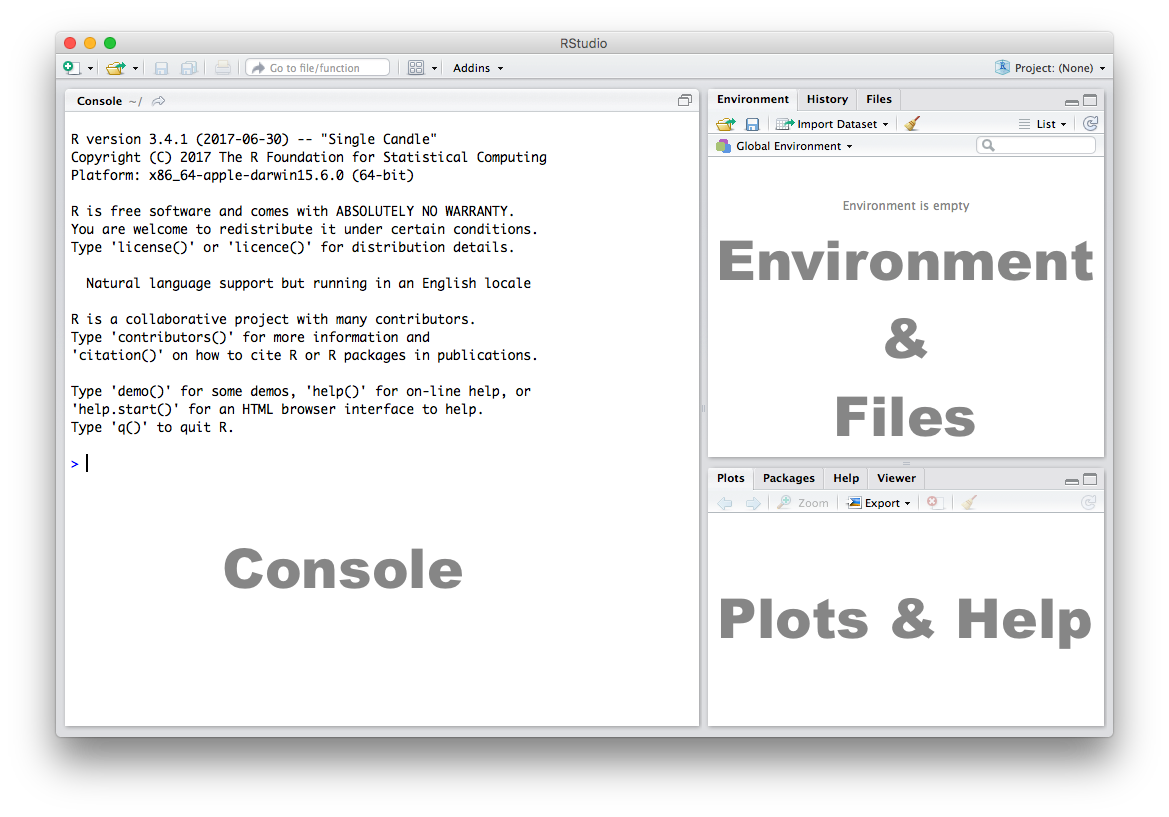
\includegraphics{./img/rstudio_default.png}
\caption{}
\end{figure}

\subsubsection{Console}\label{console}

The Console in RStudio is the simplest way to interact with R. You can
type some code at the Console and when you press ENTER, R will run that
code. Depending on what you type, you may see some output in the Console
or if you make a mistake, you may get a warning or an error message.

Let's familiarize ourselves with the console by using R as a simple
calculator:

\begin{Shaded}
\begin{Highlighting}[]
\DecValTok{2} \OperatorTok{+}\StringTok{ }\DecValTok{4}
\end{Highlighting}
\end{Shaded}

\begin{verbatim}
[1] 6
\end{verbatim}

Now that we know how to use the \texttt{+} sign for addition, let's try
some other mathematical operations such as subtraction (\texttt{-}),
multiplication (\texttt{*}), and division (\texttt{/}).

\begin{Shaded}
\begin{Highlighting}[]
\DecValTok{10} \OperatorTok{-}\StringTok{ }\DecValTok{4}
\end{Highlighting}
\end{Shaded}

\begin{verbatim}
[1] 6
\end{verbatim}

\begin{Shaded}
\begin{Highlighting}[]
\DecValTok{5} \OperatorTok{*}\StringTok{ }\DecValTok{3}
\end{Highlighting}
\end{Shaded}

\begin{verbatim}
[1] 15
\end{verbatim}

\begin{Shaded}
\begin{Highlighting}[]
\DecValTok{7} \OperatorTok{/}\StringTok{ }\DecValTok{2}
\end{Highlighting}
\end{Shaded}

\begin{verbatim}
[1] 3.5
\end{verbatim}

\begin{longtable}[]{@{}ll@{}}
\toprule
\begin{minipage}[t]{0.69\columnwidth}\raggedright\strut
You can use the cursor or arrow keys on your keyboard to edit your code
at the console:- Use the UP and DOWN keys to re-run something without
typing it again- Use the LEFT and RIGHT keys to edit\strut
\end{minipage} & \begin{minipage}[t]{0.25\columnwidth}\raggedright\strut
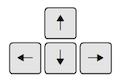
\includegraphics{./img/rstudio_cursorkeys.png}\strut
\end{minipage}\tabularnewline
\bottomrule
\end{longtable}

Take a few minutes to play around at the console and try different
things out. Don't worry if you make a mistake, you can't break anything
easily!

\subsubsection{Functions}\label{functions}

Functions are a set of instructions that carry out a specific task.
Functions often require some input and generate some output. For
example, instead of using the \texttt{+} operator for addition, we can
use the \texttt{sum} function to add two or more numbers.

\begin{Shaded}
\begin{Highlighting}[]
\KeywordTok{sum}\NormalTok{(}\DecValTok{1}\NormalTok{, }\DecValTok{4}\NormalTok{, }\DecValTok{10}\NormalTok{)}
\end{Highlighting}
\end{Shaded}

\begin{verbatim}
[1] 15
\end{verbatim}

In the example above, \texttt{1,\ 4,\ 10} are the inputs and 15 is the
output. A function always requires the use of parenthesis or round
brackets \texttt{()}. Inputs to the function are called
\textbf{arguments} and go inside the brackets. The output of a function
is displayed on the screen but we can also have the option of saving the
result of the output. More on this later.

\subsubsection{Getting Help}\label{getting-help}

Another useful function in R is \texttt{help} which we can use to
display online documentation. For example, if we wanted to know how to
use the \texttt{sum} function, we could type \texttt{help(sum)} and look
at the online documentation.

\begin{Shaded}
\begin{Highlighting}[]
\KeywordTok{help}\NormalTok{(sum)}
\end{Highlighting}
\end{Shaded}

The question mark \texttt{?} can also be used as a shortcut to access
online help.

\begin{Shaded}
\begin{Highlighting}[]
\NormalTok{?sum}
\end{Highlighting}
\end{Shaded}

\begin{figure}
\centering
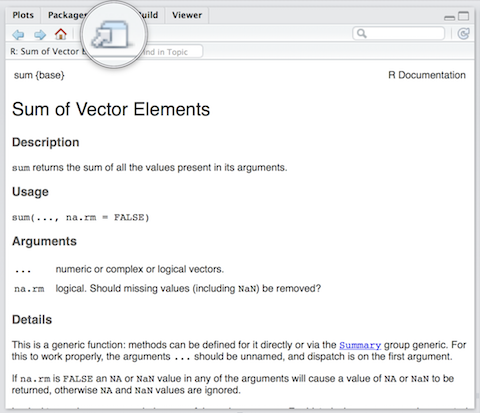
\includegraphics{./img/rstudio_help.png}
\caption{}
\end{figure}

Use the toolbar button shown in the picture above to expand and display
the help in a new window.

Help pages for functions in R follow a consistent layout generally
include these sections:

\begin{longtable}[]{@{}ll@{}}
\toprule
Description & A brief description of the function\tabularnewline
Usage & The complete syntax or grammar including all arguments
(inputs)\tabularnewline
Arguments & Explanation of each argument\tabularnewline
Details & Any relevant details about the function and its
arguments\tabularnewline
Value & The output value of the function\tabularnewline
Examples & Example of how to use the function\tabularnewline
\bottomrule
\end{longtable}

\subsubsection{The Assignment Operator}\label{the-assignment-operator}

Now we know how to provide inputs to a function using parenthesis or
round brackets \texttt{()}, but what about the output of a function?

We use the assignment operator \textbf{\texttt{\textless{}-}} for
creating or updating objects. If we wanted to save the result of adding
\texttt{sum(1,\ 4,\ 10)}, we would do the following:

\begin{Shaded}
\begin{Highlighting}[]
\NormalTok{myresult <-}\StringTok{ }\KeywordTok{sum}\NormalTok{(}\DecValTok{1}\NormalTok{, }\DecValTok{4}\NormalTok{, }\DecValTok{10}\NormalTok{)}
\end{Highlighting}
\end{Shaded}

The line above creates a new object called \texttt{myresult} in our
environment and saves the result of the \texttt{sum(1,\ 4,\ 10)} in it.
To see what's in \texttt{myresult}, just type it at the console:

\begin{Shaded}
\begin{Highlighting}[]
\NormalTok{myresult}
\end{Highlighting}
\end{Shaded}

\begin{verbatim}
[1] 15
\end{verbatim}

Take a look at the \textbf{Environment} pane in RStudio and you'll see
\texttt{myresult} there.

\begin{figure}
\centering
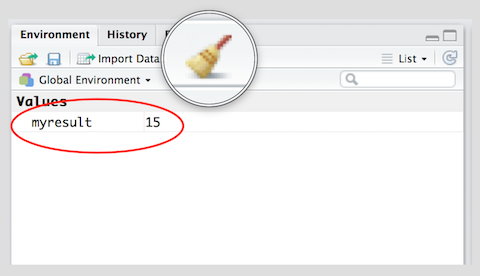
\includegraphics{./img/rstudio_env.png}
\caption{}
\end{figure}

To delete all objects from the environment, you can use the
\textbf{broom} button as shown in the picture above.

We called our object \texttt{myresult} but we can call it anything as
long as we follow a few simple rules. Object names can contain upper or
lower case letters (\texttt{A-Z}, \texttt{a-z}), numbers (\texttt{0-9}),
underscores (\texttt{\_}) or a dot (\texttt{.}) but all object names
must start with a letter. Choose names that are descriptive and easy to
type.

\begin{longtable}[]{@{}ll@{}}
\toprule
Good Object Names & Bad Object Names\tabularnewline
\midrule
\endhead
result & a\tabularnewline
myresult & x1\tabularnewline
my.result & this.name.is.just.too.long\tabularnewline
my\_result &\tabularnewline
data1 &\tabularnewline
\bottomrule
\end{longtable}

\subsubsection{Sequences}\label{sequences}

We often need to create sequences when manipulating data. For instance,
you might want to perform an operation on the first 10 rows of a dataset
so we need a way to select the range we're interested in.

There are two ways to create a sequence. Let's try to create a sequence
of numbers from 1 to 10 using the two methods:

\begin{enumerate}
\def\labelenumi{\arabic{enumi}.}
\tightlist
\item
  Using the colon \texttt{:} operator. If you're familiar with
  spreadsheets then you might've already used \texttt{:} to select
  cells, for example \texttt{A1:A20}. In R, you can use the \texttt{:}
  to create a sequence in a similar fashion:
\end{enumerate}

\begin{Shaded}
\begin{Highlighting}[]
\DecValTok{1}\OperatorTok{:}\DecValTok{10}
\end{Highlighting}
\end{Shaded}

\begin{verbatim}
 [1]  1  2  3  4  5  6  7  8  9 10
\end{verbatim}

\begin{enumerate}
\def\labelenumi{\arabic{enumi}.}
\tightlist
\item
  Using the \texttt{seq} function we get the exact same result:
\end{enumerate}

\begin{Shaded}
\begin{Highlighting}[]
\KeywordTok{seq}\NormalTok{(}\DataTypeTok{from =} \DecValTok{1}\NormalTok{, }\DataTypeTok{to =} \DecValTok{10}\NormalTok{)}
\end{Highlighting}
\end{Shaded}

\begin{verbatim}
 [1]  1  2  3  4  5  6  7  8  9 10
\end{verbatim}

The \texttt{seq} function has a number of options which control how the
sequence is generated. For example to create a sequence from 0 to 100 in
increments of \texttt{5}, we can use the optional \texttt{by} argument.
Notice how we wrote \texttt{by\ =\ 5} as the third argument. It is a
common practice to specify the name of argument when the argument is
optional. The arguments \texttt{from} and \texttt{to} are not optional,
se we can write \texttt{seq(0,\ 100,\ by\ =\ 5)} instead of
\texttt{seq(from\ =\ 0,\ to\ =\ 100,\ by\ =\ 5)}. Both, are valid ways
of achieving the same outcome. You can code whichever way you like. We
recommend to write code such that you make it easy for your future self
and others to read and understand the code.

\begin{Shaded}
\begin{Highlighting}[]
\KeywordTok{seq}\NormalTok{(}\DataTypeTok{from =} \DecValTok{0}\NormalTok{, }\DataTypeTok{to =} \DecValTok{100}\NormalTok{, }\DataTypeTok{by =} \DecValTok{5}\NormalTok{)}
\end{Highlighting}
\end{Shaded}

\begin{verbatim}
 [1]   0   5  10  15  20  25  30  35  40  45  50  55  60  65  70  75  80
[18]  85  90  95 100
\end{verbatim}

Another common use of the \texttt{seq} function is to create a sequence
of a specific length. Here, we create a sequence from 0 to 100 with
length 9, i.e., the result is a vector with 9 elements.

\begin{Shaded}
\begin{Highlighting}[]
\KeywordTok{seq}\NormalTok{(}\DataTypeTok{from =} \DecValTok{0}\NormalTok{, }\DataTypeTok{to =} \DecValTok{100}\NormalTok{, }\DataTypeTok{length.out =}  \DecValTok{9}\NormalTok{)}
\end{Highlighting}
\end{Shaded}

\begin{verbatim}
[1]   0.0  12.5  25.0  37.5  50.0  62.5  75.0  87.5 100.0
\end{verbatim}

Now it's your turn:

\begin{itemize}
\tightlist
\item
  Create a sequence of \textbf{odd} numbers between 0 and 100 and save
  it in an object called \texttt{odd\_numbers}
\end{itemize}

\begin{Shaded}
\begin{Highlighting}[]
\NormalTok{odd_numbers <-}\StringTok{ }\KeywordTok{seq}\NormalTok{(}\DecValTok{1}\NormalTok{, }\DecValTok{100}\NormalTok{, }\DecValTok{2}\NormalTok{)}
\end{Highlighting}
\end{Shaded}

\begin{itemize}
\tightlist
\item
  Next, display \texttt{odd\_numbers} on the console to verify that you
  did it correctly
\end{itemize}

\begin{Shaded}
\begin{Highlighting}[]
\NormalTok{odd_numbers}
\end{Highlighting}
\end{Shaded}

\begin{verbatim}
 [1]  1  3  5  7  9 11 13 15 17 19 21 23 25 27 29 31 33 35 37 39 41 43 45
[24] 47 49 51 53 55 57 59 61 63 65 67 69 71 73 75 77 79 81 83 85 87 89 91
[47] 93 95 97 99
\end{verbatim}

\begin{itemize}
\item
  What do the numbers in square brackets \texttt{{[}\ {]}} mean? Look at
  the number of values displayed in each line to find out the answer.
\item
  Use the \texttt{length} function to find out how many values are in
  the object \texttt{odd\_numbers}.

  \begin{itemize}
  \tightlist
  \item
    HINT: Try \texttt{help(length)} and look at the examples section at
    the end of the help screen.
  \end{itemize}
\end{itemize}

\begin{Shaded}
\begin{Highlighting}[]
\KeywordTok{length}\NormalTok{(odd_numbers)}
\end{Highlighting}
\end{Shaded}

\begin{verbatim}
[1] 50
\end{verbatim}

\subsubsection{Scripts}\label{scripts}

The Console is great for simple tasks but if you're working on a project
you would mostly likely want to save your work in some sort of a
document or a file. Scripts in R are just plain text files that contain
R code. You can edit a script just like you would edit a file in any
word processing or note-taking application.

Create a new script using the menu or the toolbar button as shown below.

\begin{figure}
\centering
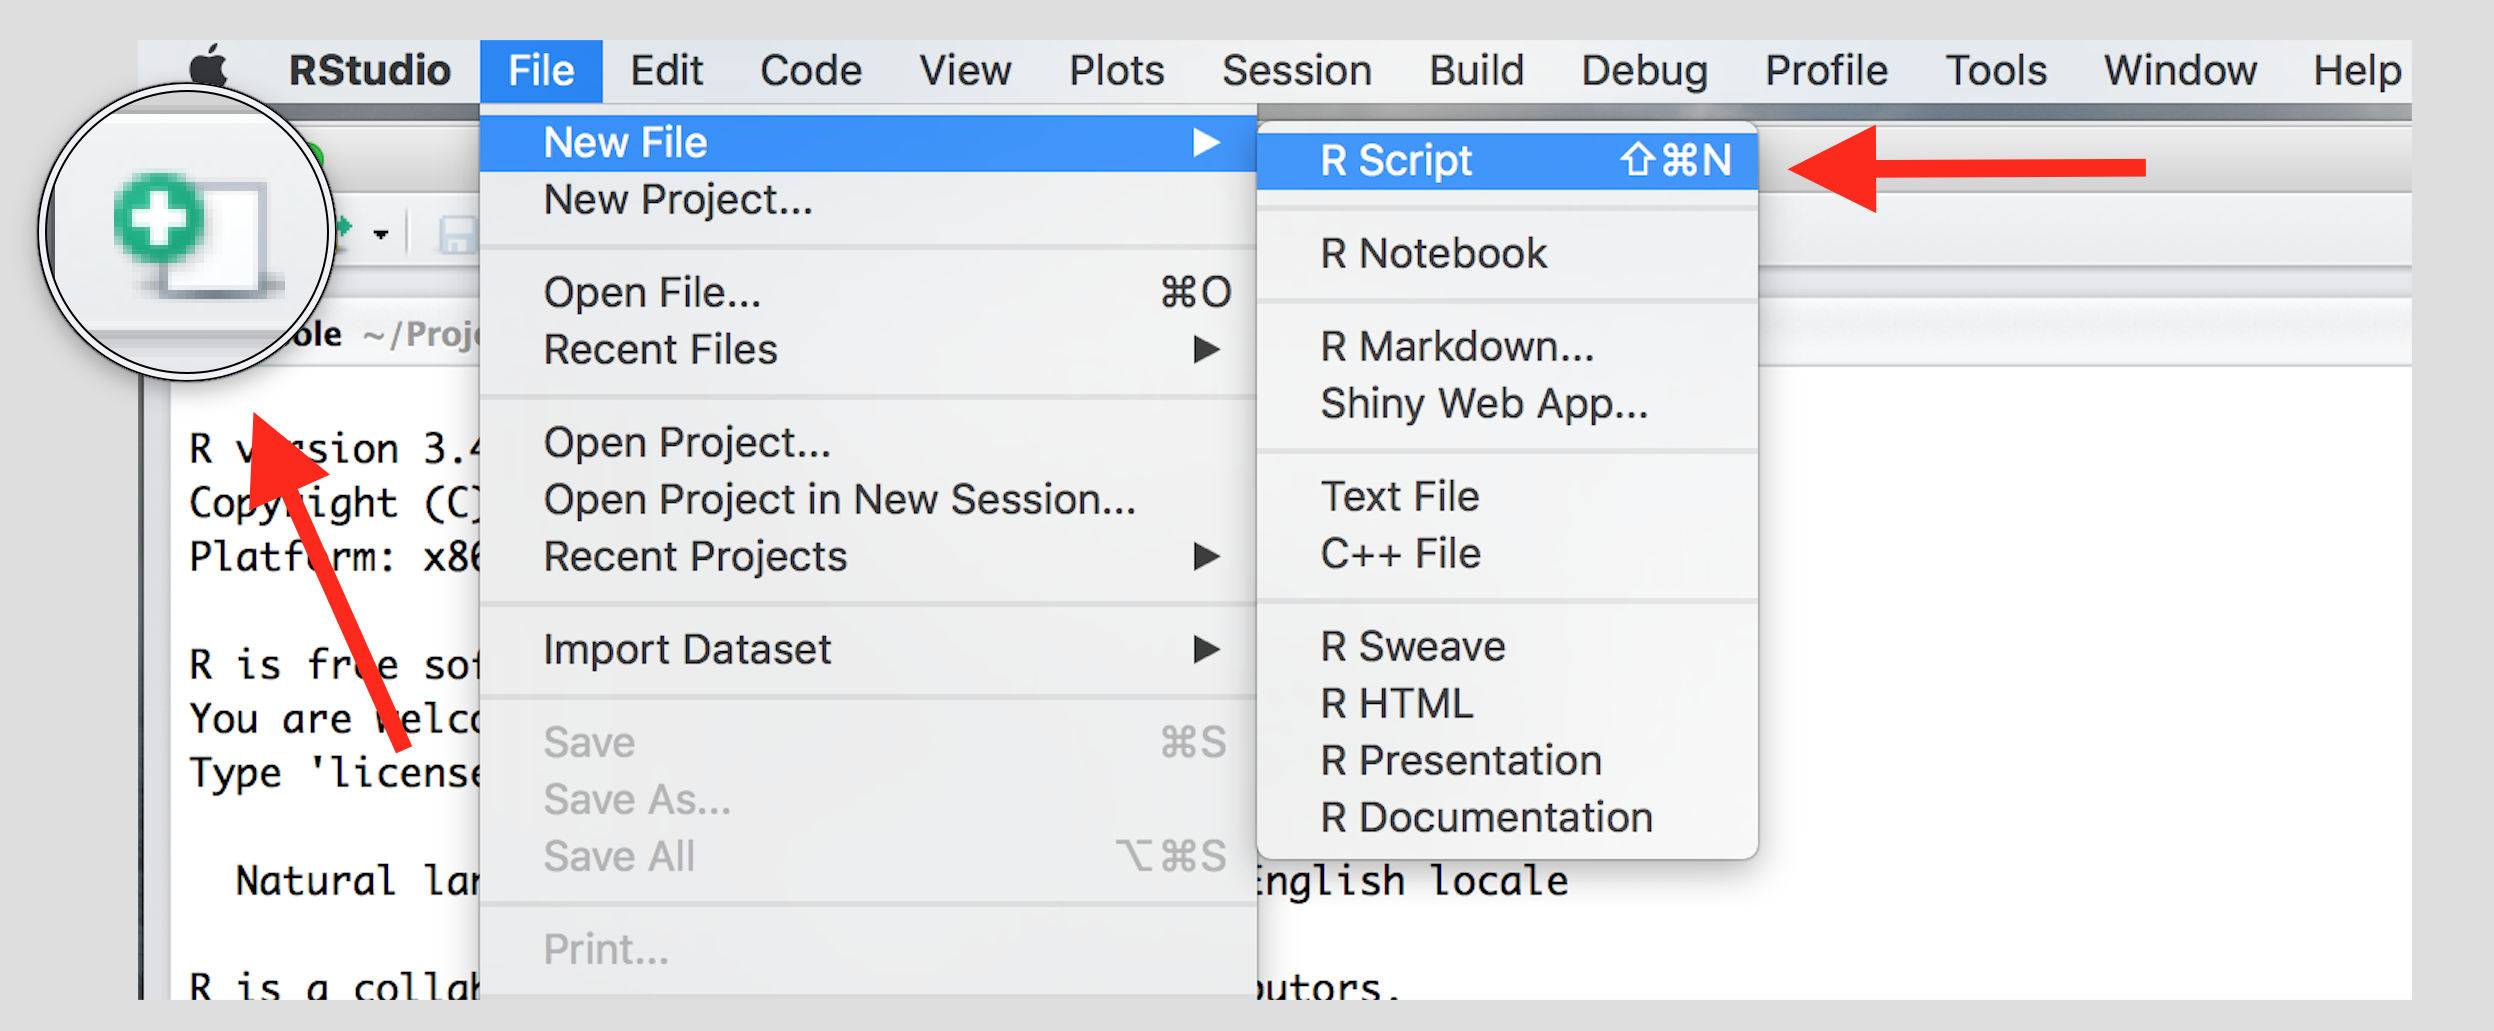
\includegraphics{./img/rstudio_newfile.png}
\caption{}
\end{figure}

Once you've created a script, it is generally a good idea to give it a
meaningful name and save it immediately. For our first session save your
script as \textbf{seminar1.R}

\begin{longtable}[]{@{}ll@{}}
\toprule
\begin{minipage}[t]{0.52\columnwidth}\raggedright\strut
Familiarize yourself with the script window in RStudio, and especially
the two buttons labeled \textbf{Run} and \textbf{Source}\strut
\end{minipage} & \begin{minipage}[t]{0.42\columnwidth}\raggedright\strut
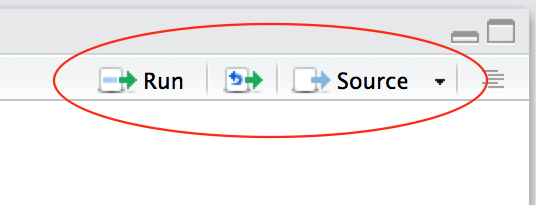
\includegraphics{./img/rstudio_script.png}\strut
\end{minipage}\tabularnewline
\bottomrule
\end{longtable}

There are a few different ways to run your code from a script.

\begin{longtable}[]{@{}ll@{}}
\toprule
\begin{minipage}[t]{0.24\columnwidth}\raggedright\strut
One line at a time\strut
\end{minipage} & \begin{minipage}[t]{0.70\columnwidth}\raggedright\strut
Place the cursor on the line you want to run and hit CTRL-ENTER or use
the \textbf{Run} button\strut
\end{minipage}\tabularnewline
\begin{minipage}[t]{0.24\columnwidth}\raggedright\strut
Multiple lines\strut
\end{minipage} & \begin{minipage}[t]{0.70\columnwidth}\raggedright\strut
Select the lines you want to run and hit CTRL-ENTER or use the
\textbf{Run} button\strut
\end{minipage}\tabularnewline
\begin{minipage}[t]{0.24\columnwidth}\raggedright\strut
Entire script\strut
\end{minipage} & \begin{minipage}[t]{0.70\columnwidth}\raggedright\strut
Use the \textbf{Source} button\strut
\end{minipage}\tabularnewline
\bottomrule
\end{longtable}

\subsubsection{Central Tendency}\label{central-tendency}

The appropriate measure of central tendency depends on the level of
measurement of the variable. To recap:

\begin{longtable}[]{@{}ll@{}}
\toprule
Level of measurement & Appropriate measure of central
tendency\tabularnewline
\midrule
\endhead
Continuous & arithmetic mean (or average)\tabularnewline
Ordered & median (or the central observation)\tabularnewline
Nominal & mode (the most frequent value)\tabularnewline
\bottomrule
\end{longtable}

\paragraph{Mean}\label{mean}

We calculate the average grade on our eleven homework assignments in
statistics 1. We create our vector of 11 (fake) grades first using the
\texttt{c()} function, where \texttt{c} stands for collect or
concatenate.

\begin{Shaded}
\begin{Highlighting}[]
\NormalTok{hw.grades <-}\StringTok{ }\KeywordTok{c}\NormalTok{(}\DecValTok{80}\NormalTok{, }\DecValTok{90}\NormalTok{, }\DecValTok{85}\NormalTok{, }\DecValTok{71}\NormalTok{, }\DecValTok{69}\NormalTok{, }\DecValTok{85}\NormalTok{, }\DecValTok{83}\NormalTok{, }\DecValTok{88}\NormalTok{, }\DecValTok{99}\NormalTok{, }\DecValTok{81}\NormalTok{, }\DecValTok{92}\NormalTok{)}
\end{Highlighting}
\end{Shaded}

We now take the sum of the grades.

\begin{Shaded}
\begin{Highlighting}[]
\NormalTok{sum.hw.grades <-}\StringTok{ }\KeywordTok{sum}\NormalTok{(hw.grades)}
\end{Highlighting}
\end{Shaded}

We also take the number of grades

\begin{Shaded}
\begin{Highlighting}[]
\NormalTok{number.hw.grades <-}\StringTok{ }\KeywordTok{length}\NormalTok{(hw.grades) }
\end{Highlighting}
\end{Shaded}

The mean is the sum of grades over the number of grades.

\begin{Shaded}
\begin{Highlighting}[]
\NormalTok{sum.hw.grades }\OperatorTok{/}\StringTok{ }\NormalTok{number.hw.grades}
\end{Highlighting}
\end{Shaded}

\begin{verbatim}
[1] 83.90909
\end{verbatim}

R provides us with an even easier way to do the same with a function
called \href{http://bit.ly/R_mean}{\texttt{mean()}}.

\begin{Shaded}
\begin{Highlighting}[]
\KeywordTok{mean}\NormalTok{(hw.grades)}
\end{Highlighting}
\end{Shaded}

\begin{verbatim}
[1] 83.90909
\end{verbatim}

\paragraph{Median}\label{median}

The median is the appropriate measure of central tendency for ordinal
variables. Ordinal means that there is a rank ordering but not equally
spaced intervals between values of the variable. Education is a common
example. In education, more education is better. But the difference
between primary school and secondary school is not the same as the
difference between secondary school and an undergraduate degree.

Let's generate a fake example with 100 people. We use numbers to code
different levels of education.

\begin{longtable}[]{@{}lll@{}}
\toprule
Code & Meaning & Frequency in our data\tabularnewline
0 & no education & 1\tabularnewline
1 & primary school & 5\tabularnewline
2 & secondary school & 55\tabularnewline
3 & undergraduate degree & 20\tabularnewline
4 & postgraduate degree & 10\tabularnewline
5 & doctorate & 9\tabularnewline
\bottomrule
\end{longtable}

We introduce a new function to create a vector. The function
\texttt{rep()}, replicates elements of a vector. Its arguments are the
item \texttt{x} to be replicated and the number of \texttt{times} to
replicate. Below, we create the variable education with the frequency of
education level indicated above. Note that the arguments \texttt{x} and
\texttt{times} do not have to be written out.

\begin{Shaded}
\begin{Highlighting}[]
\NormalTok{edu <-}\StringTok{ }\KeywordTok{c}\NormalTok{( }\KeywordTok{rep}\NormalTok{(}\DataTypeTok{x=}\DecValTok{0}\NormalTok{, }\DataTypeTok{times=}\DecValTok{1}\NormalTok{), }\KeywordTok{rep}\NormalTok{(}\DataTypeTok{x=}\DecValTok{1}\NormalTok{, }\DataTypeTok{times=}\DecValTok{5}\NormalTok{), }\KeywordTok{rep}\NormalTok{(}\DataTypeTok{x=}\DecValTok{2}\NormalTok{, }\DataTypeTok{times=}\DecValTok{55}\NormalTok{),}
          \KeywordTok{rep}\NormalTok{(}\DataTypeTok{x=}\DecValTok{3}\NormalTok{, }\DataTypeTok{times=}\DecValTok{20}\NormalTok{), }\KeywordTok{rep}\NormalTok{(}\DecValTok{4}\NormalTok{,}\DecValTok{10}\NormalTok{), }\KeywordTok{rep}\NormalTok{(}\DecValTok{5}\NormalTok{,}\DecValTok{9}\NormalTok{) )}
\end{Highlighting}
\end{Shaded}

The median level of education is the level where 50 percent of the
observations have a lower or equal level of education and 50 percent
have a higher or equal level of education. That means that the median
splits the data in half.

We use the \href{http://bit.ly/R_median}{\texttt{median()}} function for
finding the median.

\begin{Shaded}
\begin{Highlighting}[]
\KeywordTok{median}\NormalTok{(edu)}
\end{Highlighting}
\end{Shaded}

\begin{verbatim}
[1] 2
\end{verbatim}

The median level of education is secondary school.

\paragraph{Mode}\label{mode}

The mode is the appropriate measure of central tendency if the level of
measurement is nominal. Nominal means that there is no ordering implicit
in the values that a variable takes on. We create data from 1000 (fake)
voters in the United Kingdom who each express their preference on
remaining in or leaving the European Union. The options are leave or
stay. Leaving is not greater than staying and vice versa (even though we
all order the two options normatively).

\begin{longtable}[]{@{}lll@{}}
\toprule
Code & Meaning & Frequency in our data\tabularnewline
0 & leave & 509\tabularnewline
1 & stay & 491\tabularnewline
\bottomrule
\end{longtable}

\begin{Shaded}
\begin{Highlighting}[]
\NormalTok{stay <-}\StringTok{ }\KeywordTok{c}\NormalTok{(}\KeywordTok{rep}\NormalTok{(}\DecValTok{0}\NormalTok{, }\DecValTok{509}\NormalTok{), }\KeywordTok{rep}\NormalTok{(}\DecValTok{1}\NormalTok{, }\DecValTok{491}\NormalTok{))}
\end{Highlighting}
\end{Shaded}

The mode is the most common value in the data. There is no mode function
in R. The most straightforward way to determine the mode is to use the
\href{http://bit.ly/R_table}{\texttt{table()}} function. It returns a
frequency table. We can easily see the mode in the table. As your coding
skills increase, you will see other ways of recovering the mode from a
vector.

\begin{Shaded}
\begin{Highlighting}[]
\KeywordTok{table}\NormalTok{(stay)}
\end{Highlighting}
\end{Shaded}

\begin{verbatim}
stay
  0   1 
509 491 
\end{verbatim}

The mode is leaving the EU because the number of `leavers' (0) is
greater than the number of `remainers' (1).

\subsubsection{Dispersion}\label{dispersion}

The appropriate measure of dispersion depends on the level of
measurement of the variable we wish to describe.

\begin{longtable}[]{@{}ll@{}}
\toprule
Level of measurement & Appropriate measure of dispersion\tabularnewline
\midrule
\endhead
Continuous & variance and/or standard deviation\tabularnewline
Ordered & range or interquartile range\tabularnewline
Nominal & proportion in each category\tabularnewline
\bottomrule
\end{longtable}

\paragraph{Variance and standard
deviation}\label{variance-and-standard-deviation}

Both the variance and the standard deviation tell by how much an average
realisation of a variable differs from the mean of that variable. Let's
assume that our variable is income in the UK. Let's assume that its mean
is 35 000 per year. We also assume that the average deviation from 35
000 is 5 000. If we ask 100 people in the UK at random about their
income, we get 100 different answers. If we average the differences
betweeen the 100 answers and 35 000, we would get 5 000. Suppose that
the average income in France is also 35 000 per year but the average
deviation is 10 000 instead. This would imply that income is more
equally distributed in the UK than in France.

Dispersion is important to describe data as this example illustrates.
Although, mean income in our hypothetical example is the same in France
and the UK, the distribution is tighter in the UK. The figure below
illustrates our example:

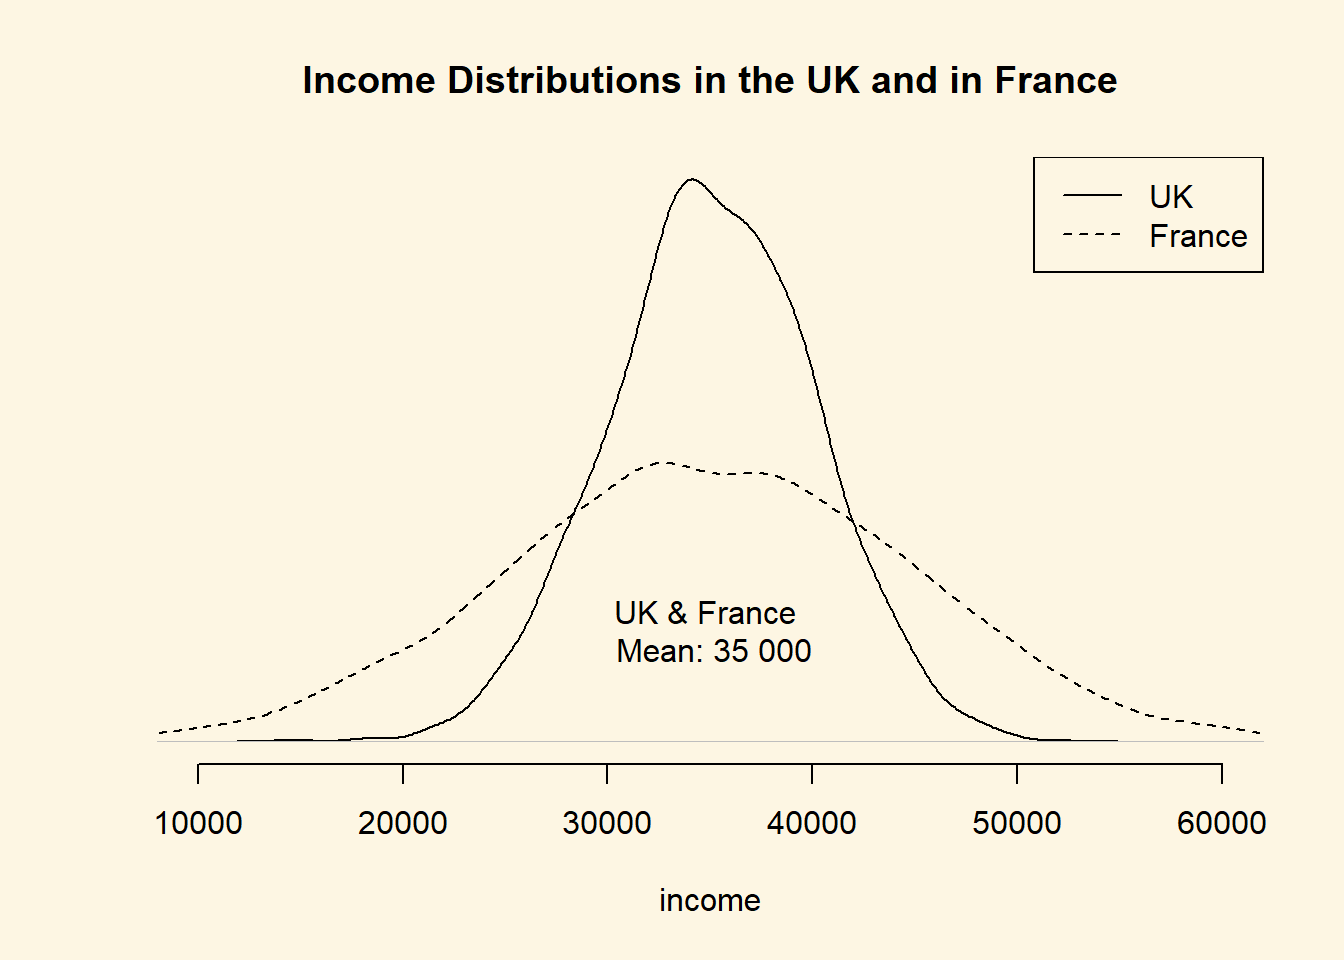
\includegraphics{statistics1_files/figure-latex/unnamed-chunk-27-1.pdf}

The variance gives us an idea about the variability of data. The formula
for the variance in the population is
\[ \frac{\sum_{i=1}^n(x_i - \mu_x)^2}{n}\]

The formula for the variance in a sample adjusts for sampling
variability, i.e., uncertainty about how well our sample reflects the
population by subtracting 1 in the denominator. Subtracting 1 will have
next to no effect if n is large but the effect increases the smaller n.
The smaller n, the larger the sample variance. The intuition is, that in
smaller samples, we are less certain that our sample reflects the
population. We, therefore, adjust variability of the data upwards. The
formula is

\[ \frac{\sum_{i=1}^n(x_i - \bar{x})^2}{n-1}\]

Notice the different notation for the mean in the two formulas. We write
\(\mu_x\) for the mean of x in the population and \(\bar{x}\) for the
mean of x in the sample. Notation is, however, unfortunately not always
consistent.

Take a minute to think your way through the formula. There are 4 setps:
(1), In the numerator, we subtract the mean of x from some realisation
of x. (2), We square the deviations from the mean because we want
positive numbers only. (3) We sum the squared deviations. (4) We divide
the sum by \((n-1)\). Below we show this for the homework example. In
the last row, we add a 5th step. We take the square root in order to
return to the orginial units of the homework grades.

\begin{longtable}[]{@{}llll@{}}
\toprule
Obs & Var & Dev. from mean & Squared dev. from mean\tabularnewline
\midrule
\endhead
i & grade & \(x_i-\bar{x}\) & \((x_i-\bar{x})^2\)\tabularnewline
1 & 80 & -3.9090909 & 15.2809917\tabularnewline
2 & 90 & 6.0909091 & 37.0991736\tabularnewline
3 & 85 & 1.0909091 & 1.1900826\tabularnewline
4 & 71 & -12.9090909 & 166.6446281\tabularnewline
5 & 69 & -14.9090909 & 222.2809917\tabularnewline
6 & 85 & 1.0909091 & 1.1900826\tabularnewline
7 & 83 & -0.9090909 & 0.8264463\tabularnewline
8 & 88 & 4.0909091 & 16.7355372\tabularnewline
9 & 99 & 15.0909091 & 227.7355372\tabularnewline
10 & 81 & -2.9090909 & 8.4628099\tabularnewline
11 & 92 & 8.0909091 & 65.4628099\tabularnewline
\(\sum_{i=1}^n\) & & & 762.9090909\tabularnewline
\(\div n-1\) & & & 76.2909091\tabularnewline
\(\sqrt{}\) & & & 8.7344667\tabularnewline
\bottomrule
\end{longtable}

Our first grade (80) is below the mean (83.9090909). The sum is, thus,
negative. Our second grade (90) is above the mean, so that the sum is
positive. Both are deviations from the mean (think of them as
distances). Our sum shall reflect the total sum of distances and
distances must be positive. Hence, we square the distances from the
mean. Having done this for all eleven observations, we sum the squared
distances. Dividing by 10 (with the sample adjustment), gives us the
average squared deviation. This is the variance. The units of the
variance---squared deviations---are somewhat awkward. We return to this
in a moment.

We take the variance in R by using the
\href{http://bit.ly/R_var}{\texttt{var()}} function. By default
\texttt{var()} takes the sample variance.

\begin{Shaded}
\begin{Highlighting}[]
\KeywordTok{var}\NormalTok{(hw.grades)}
\end{Highlighting}
\end{Shaded}

\begin{verbatim}
[1] 76.29091
\end{verbatim}

The average squared difference form our mean grade is 76.2909091. But
what does that mean? We would like to get rid of the square in our
units. That's what the standard deviation does. The standard deviation
is the square root over the variance.

\[ \sqrt{\frac{\sum_{i=1}^n(x_i - \bar{x})^2}{n-1}}\]

We get the average deviation from our mean grade (83.9090909) with the
\href{http://bit.ly/R_sd}{\texttt{sd()}} function.

\begin{Shaded}
\begin{Highlighting}[]
\KeywordTok{sd}\NormalTok{(hw.grades)}
\end{Highlighting}
\end{Shaded}

\begin{verbatim}
[1] 8.734467
\end{verbatim}

The standard deviation is much more intuitive than the variance because
its units are the same as the units of the variable we are interested
in. ``Why teach us about this awful variance then'', you ask.
Mathematically, we have to compute the variance before getting the
standard deviation. We recommend that you use the standard deviation to
describe the variability of your continuous data.

Note: We used the sample variance and sample standard deviation
formulas. If the eleven assignments represent the population, we would
use the population variance formula. Whether the 11 cases represent a
sample or the population depends on what we want to know. If we want
learn about all students' assignments or future assignments, the 11
cases are a sample.

\paragraph{Range and interquartile
range}\label{range-and-interquartile-range}

The proper measure of dispersion of an ordinal variable is the range or
the interquartile range. The interquartile range is usually the
preferred measure because the range is strongly affected by outlying
cases.

Let's take the range first. We get back to our education example. In R,
we use the \href{http://bit.ly/R_range}{\texttt{range()}} function to
compute the range.

\begin{Shaded}
\begin{Highlighting}[]
\KeywordTok{range}\NormalTok{(edu)}
\end{Highlighting}
\end{Shaded}

\begin{verbatim}
[1] 0 5
\end{verbatim}

Our data ranges from no education all the way to those with a doctorate.
However, no education is not a common value. Only one person in our
sample did not have any education. The interquartile range is the range
from the 25th to the 75th percentiles, i.e., it contains the central 50
percent of the distribution.

The 25th percentile is the value of education that 25 percent or fewer
people have (when we order education from lowest to highest). We use the
\href{http://bit.ly/R_quantile}{\texttt{quantile()}} function in R to
get percentiles. The function takes two arguments: \texttt{x} is the
data vector and \texttt{probs} is the percentile.

\begin{Shaded}
\begin{Highlighting}[]
\KeywordTok{quantile}\NormalTok{(edu, }\FloatTok{0.25}\NormalTok{) }\CommentTok{# 25th percentile}
\end{Highlighting}
\end{Shaded}

\begin{verbatim}
25% 
  2 
\end{verbatim}

\begin{Shaded}
\begin{Highlighting}[]
\KeywordTok{quantile}\NormalTok{(edu, }\FloatTok{0.75}\NormalTok{) }\CommentTok{# 75th percentile}
\end{Highlighting}
\end{Shaded}

\begin{verbatim}
75% 
  3 
\end{verbatim}

Therefore, the interquartile range is from 2, secondary school to 3,
undergraduate degree.

\paragraph{Proportion in each
category}\label{proportion-in-each-category}

To describe the distribution of our nominal variable, support for
remaining in the European Union, we use the proportions in each
category.

Recall, that we looked at the frequency table to determine the mode:

\begin{Shaded}
\begin{Highlighting}[]
\KeywordTok{table}\NormalTok{(stay)}
\end{Highlighting}
\end{Shaded}

\begin{verbatim}
stay
  0   1 
509 491 
\end{verbatim}

To get the proportions in each category, we divide the values in the
table, i.e., 509 and 491, by the sum of the table, i.e., 1000.

\begin{Shaded}
\begin{Highlighting}[]
\KeywordTok{table}\NormalTok{(stay) }\OperatorTok{/}\StringTok{ }\KeywordTok{sum}\NormalTok{(}\KeywordTok{table}\NormalTok{(stay))}
\end{Highlighting}
\end{Shaded}

\begin{verbatim}
stay
    0     1 
0.509 0.491 
\end{verbatim}

\subsubsection{Exercises}\label{exercises}

\begin{enumerate}
\def\labelenumi{\arabic{enumi}.}
\tightlist
\item
  Create a script and call it assignment01. Save your script.
\item
  Download this
  \href{https://www.rstudio.com/wp-content/uploads/2016/06/r-cheat-sheet.pdf}{cheat-sheet}
  and go over it. You won't understand most of it right a away. But it
  will become a useful resource. Look at it often.
\item
  Calculate the square root of 1369 using the \texttt{sqrt()} function.
\item
  Square the number 13 using the \texttt{\^{}} operator.
\item
  What is the result of summing all numbers from 1 to 100?
\end{enumerate}

We take a sample of yearly income in Berlin. The values that we got are:
19395, 22698, 40587, 25705, 26292, 42150, 29609, 12349, 18131, 20543,
37240, 28598, 29007, 26106, 19441, 42869, 29978, 5333, 32013, 20272,
14321, 22820, 14739, 17711, 18749.

\begin{enumerate}
\def\labelenumi{\arabic{enumi}.}
\setcounter{enumi}{5}
\tightlist
\item
  Create the variable \texttt{income} with the values form our Berlin
  sample in R.
\item
  Describe Berlin income using the appropriate measures of central
  tendency and dispersion.
\item
  Compute the average deviation without using the \texttt{sd()}
  function.
\end{enumerate}

Take a look at the Sunday Question (who would you vote for if the
general election were next Sunday?) by following this link
\href{https://www.wahlrecht.de/umfragen/}{Sunday Question Germany}. You
should be able to translate the website into English by right clicking
in your browser and clicking ``Translate to English.''

\begin{enumerate}
\def\labelenumi{\arabic{enumi}.}
\setcounter{enumi}{8}
\tightlist
\item
  What is the level of measurement of the variable in the Sunday
  Question?
\item
  Take the most recent poll and describe what you see in terms of
  central tendency and dispersion.
\item
  Save your script, which should now include the answers to all the
  exercises.
\item
  Source your script, i.e.~run the entire script without error message.
  Clean your script if you get error messages.
\end{enumerate}

\subsection{Solutions}\label{solutions}

\subsubsection{Exercise 3}\label{exercise-3}

Calculate the square root of 1369 using the \texttt{sqrt()} function.

\begin{Shaded}
\begin{Highlighting}[]
\KeywordTok{sqrt}\NormalTok{(}\DecValTok{1369}\NormalTok{)}
\end{Highlighting}
\end{Shaded}

\begin{verbatim}
[1] 37
\end{verbatim}

\subsubsection{Exercise 4}\label{exercise-4}

Square the number 13 using the \texttt{\^{}} operator.

\begin{Shaded}
\begin{Highlighting}[]
\DecValTok{13}\OperatorTok{^}\DecValTok{2}
\end{Highlighting}
\end{Shaded}

\begin{verbatim}
[1] 169
\end{verbatim}

\subsubsection{Exercise 5}\label{exercise-5}

What is the result of summing all numbers from 1 to 100?

\begin{Shaded}
\begin{Highlighting}[]
\CommentTok{# sequence of numbers from 1 to 100 in steps of 1}
\NormalTok{numbers_1_to_}\DecValTok{100}\NormalTok{ <-}\StringTok{ }\KeywordTok{seq}\NormalTok{(}\DataTypeTok{from =} \DecValTok{1}\NormalTok{, }\DataTypeTok{to =} \DecValTok{100}\NormalTok{, }\DataTypeTok{by =} \DecValTok{1}\NormalTok{)}
\CommentTok{# sum over the vector}
\NormalTok{result <-}\StringTok{ }\KeywordTok{sum}\NormalTok{(numbers_1_to_}\DecValTok{100}\NormalTok{)}
\CommentTok{# print the result}
\NormalTok{result}
\end{Highlighting}
\end{Shaded}

\begin{verbatim}
[1] 5050
\end{verbatim}

The result is 5050.

\subsubsection{Exercise 6}\label{exercise-6}

Create the variable \emph{income} with the values form our Berlin sample
in R.

\begin{Shaded}
\begin{Highlighting}[]
\CommentTok{# create the income variable using the c() function}
\NormalTok{income <-}\StringTok{ }\KeywordTok{c}\NormalTok{(}
  \DecValTok{19395}\NormalTok{, }\DecValTok{22698}\NormalTok{, }\DecValTok{40587}\NormalTok{, }\DecValTok{25705}\NormalTok{, }\DecValTok{26292}\NormalTok{, }\DecValTok{42150}\NormalTok{, }\DecValTok{29609}\NormalTok{, }\DecValTok{12349}\NormalTok{, }\DecValTok{18131}\NormalTok{, }
  \DecValTok{20543}\NormalTok{, }\DecValTok{37240}\NormalTok{, }\DecValTok{28598}\NormalTok{, }\DecValTok{29007}\NormalTok{, }\DecValTok{26106}\NormalTok{, }\DecValTok{19441}\NormalTok{, }\DecValTok{42869}\NormalTok{, }\DecValTok{29978}\NormalTok{, }\DecValTok{5333}\NormalTok{, }
  \DecValTok{32013}\NormalTok{, }\DecValTok{20272}\NormalTok{, }\DecValTok{14321}\NormalTok{, }\DecValTok{22820}\NormalTok{, }\DecValTok{14739}\NormalTok{, }\DecValTok{17711}\NormalTok{, }\DecValTok{18749}
\NormalTok{)}
\end{Highlighting}
\end{Shaded}

\subsubsection{Exercise 7}\label{exercise-7}

Describe Berlin income using the appropriate measures of central
tendency and dispersion.

We use the mean for the central tendency of \emph{income}. The variable
is interval scaled and the mean is the appropriate measure of central
tendency for interval scaled variables. Our \emph{income} variable is
also normally distributed. Income distributions in most countries are
right skewed. Therefore, the central tendency of income is often
described using the median.

When asked, e.g., in an exam, to describe the central tendency of an
interval scaled variable, use the mean. You can also use the median if
you tell us why.

\begin{Shaded}
\begin{Highlighting}[]
\CommentTok{# central tendency of income}
\KeywordTok{mean}\NormalTok{(income)}
\end{Highlighting}
\end{Shaded}

\begin{verbatim}
[1] 24666.24
\end{verbatim}

\begin{Shaded}
\begin{Highlighting}[]
\CommentTok{# dispersion}
\KeywordTok{sd}\NormalTok{(income)}
\end{Highlighting}
\end{Shaded}

\begin{verbatim}
[1] 9467.383
\end{verbatim}

Average income in our Berlin sample is 24666.24. The average difference
from that value is 9467.38.

\subsubsection{Exercise 8}\label{exercise-8}

Compute the average deviation without using the sd() function.

We do this in several steps. First, we compute the mean.

\begin{Shaded}
\begin{Highlighting}[]
\NormalTok{mean.income <-}\StringTok{ }\KeywordTok{sum}\NormalTok{(income) }\OperatorTok{/}\StringTok{ }\KeywordTok{length}\NormalTok{(income)}

\CommentTok{# let's print the mean}
\NormalTok{mean.income}
\end{Highlighting}
\end{Shaded}

\begin{verbatim}
[1] 24666.24
\end{verbatim}

Second, we take the differences between each individual realisation of
income and the mean of \emph{income}. The result must be a vector with
the same amount of elements as the \emph{income} vector.

\begin{Shaded}
\begin{Highlighting}[]
\CommentTok{# individual differences between each realisation of income and the mean of income}
\NormalTok{diffs.from.mean <-}\StringTok{ }\NormalTok{income }\OperatorTok{-}\StringTok{ }\NormalTok{mean.income}

\CommentTok{# let's print the vector of differences}
\NormalTok{diffs.from.mean}
\end{Highlighting}
\end{Shaded}

\begin{verbatim}
 [1]  -5271.24  -1968.24  15920.76   1038.76   1625.76  17483.76   4942.76
 [8] -12317.24  -6535.24  -4123.24  12573.76   3931.76   4340.76   1439.76
[15]  -5225.24  18202.76   5311.76 -19333.24   7346.76  -4394.24 -10345.24
[22]  -1846.24  -9927.24  -6955.24  -5917.24
\end{verbatim}

You may be surprised that this works. After all, \emph{income} is a
vector with 25 elements and \emph{mean.income} is a scalar (only one
value). R treats all variables as vectors. It notices that
\emph{mean.income} is a shorter vector than \emph{income}. The former
has 1 element and the latter 25. The vector \emph{mean.income} is
recycled, so that it has the same length as \emph{income} where each
element is the same: the mean of \emph{income}. If you did not
understand this don't worry. The important thing is that it works.

Our next step is to square the differences from the mean.

\begin{Shaded}
\begin{Highlighting}[]
\CommentTok{# square each element in the diffs.from.mean vector}
\NormalTok{squared.diffs.from.mean <-}\StringTok{ }\NormalTok{diffs.from.mean}\OperatorTok{^}\DecValTok{2}

\CommentTok{# print the squared vecto}
\NormalTok{squared.diffs.from.mean}
\end{Highlighting}
\end{Shaded}

\begin{verbatim}
 [1]  27785971   3873969 253470599   1079022   2643096 305681864  24430876
 [8] 151714401  42709362  17001108 158099441  15458737  18842197   2072909
[15]  27303133 331340472  28214794 373774169  53974882  19309345 107023991
[22]   3408602  98550094  48375363  35013729
\end{verbatim}

We squared each individual element in the vector. Therefore, our new
variable \emph{squared.diffs.from.mean} still has 25 elements.

Squaring a value does two things. First, all values in our vector have
become positive. Second, the marginal increase increases with distance,
i.e., values that are close to the mean are only somewhat larger whereas
values that are further from the mean become way larger. To see this,
lets plot the square (we haven't shown you the plot function yet, but we
will do this next seminar).

\begin{Shaded}
\begin{Highlighting}[]
\CommentTok{# a vector of x values from negative 100 to positive 100}
\NormalTok{a <-}\StringTok{ }\KeywordTok{seq}\NormalTok{(}\DataTypeTok{from =} \OperatorTok{-}\DecValTok{100}\NormalTok{, }\DataTypeTok{to =} \DecValTok{100}\NormalTok{, }\DataTypeTok{length.out =} \DecValTok{200}\NormalTok{)}

\CommentTok{# the square of that vector}
\NormalTok{b <-}\StringTok{ }\NormalTok{a}\OperatorTok{^}\DecValTok{2}

\CommentTok{# we plot the input vector a against b, where b is on the y-axis}
\KeywordTok{plot}\NormalTok{(}
  \DataTypeTok{x =}\NormalTok{ a, }\CommentTok{# x-axis values}
  \DataTypeTok{y =}\NormalTok{ b, }\CommentTok{# y-axis values}
  \DataTypeTok{bty =} \StringTok{"n"}\NormalTok{, }\CommentTok{# no border around plot}
  \DataTypeTok{type =} \StringTok{"l"}\NormalTok{, }\CommentTok{# connect individual dots to a line}
  \DataTypeTok{xlab =} \StringTok{"input values from vector a"}\NormalTok{, }\CommentTok{# x axis label}
  \DataTypeTok{ylab =} \StringTok{"b = a^2"} \CommentTok{# y axis label}
\NormalTok{)}
\end{Highlighting}
\end{Shaded}

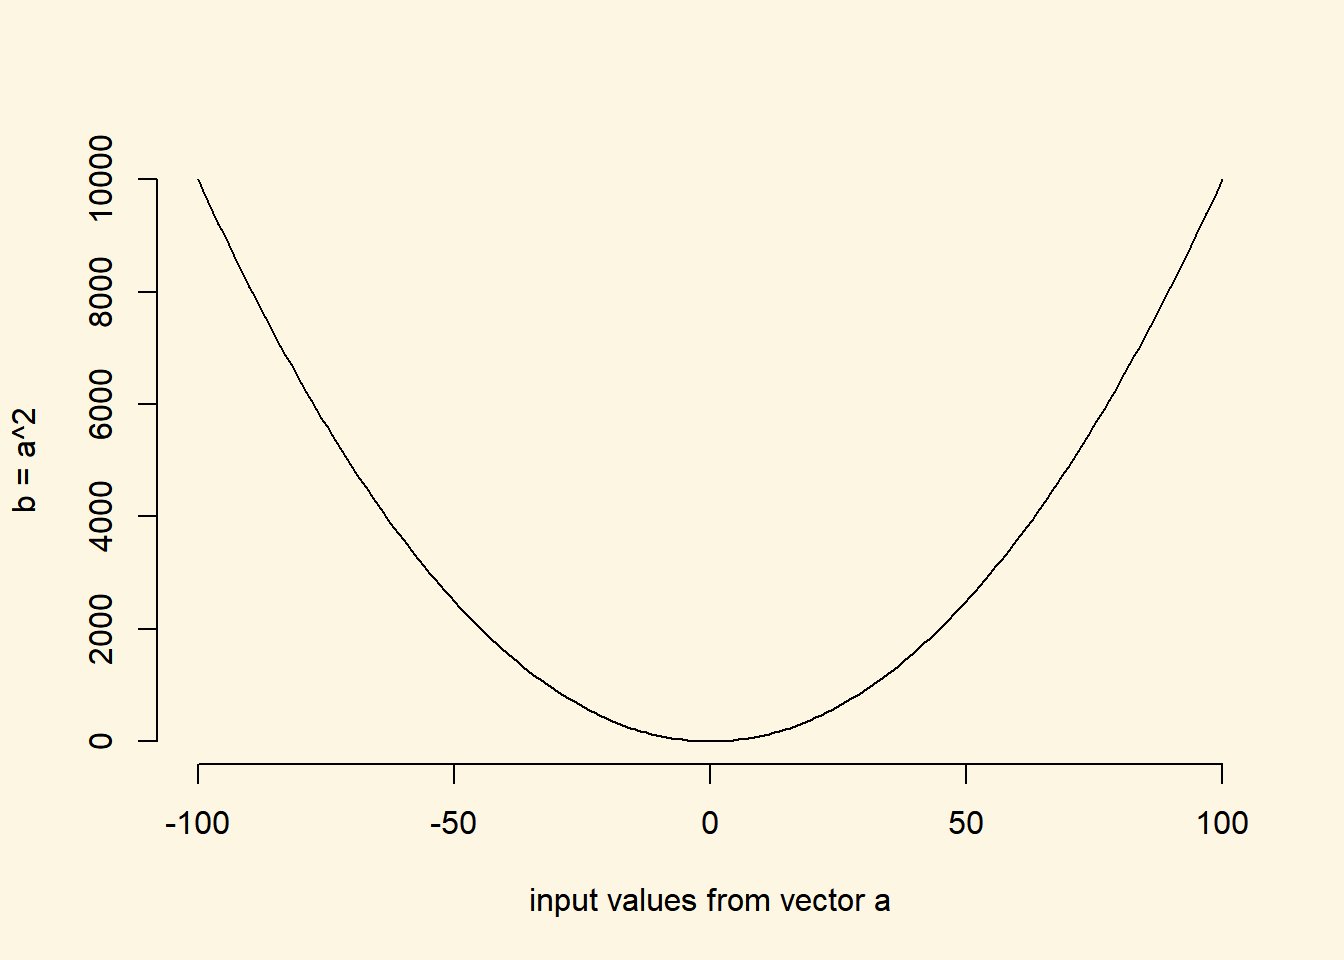
\includegraphics{statistics1_files/figure-latex/unnamed-chunk-45-1.pdf}

In this plot, you should see that the slope of the line increases, the
further we are from 0. We are taking individual differences from the
mean. Hence, if a value is exactly at the mean, the difference is zero.
The further, the value is from the mean (in any direction), the larger
the output value.

We will sum over the individual elements in the next step. Hence, values
that are further from the mean have a larger impact on the sum than
values that are closer to the mean.

In the next step, we take the sum over our squared deviations from the
mean

\begin{Shaded}
\begin{Highlighting}[]
\CommentTok{# sum over squared deviations vector}
\NormalTok{sum.of.squared.deviations <-}\StringTok{ }\KeywordTok{sum}\NormalTok{(squared.diffs.from.mean)}

\CommentTok{# print the sum}
\NormalTok{sum.of.squared.deviations}
\end{Highlighting}
\end{Shaded}

\begin{verbatim}
[1] 2151152127
\end{verbatim}

By summing over all elements of a vector, we end up with a scalar. The
sum is 2151152126.56.

We divide the sum of squared deviations by \(n-1\). Recall, that \(n\)
is the number of observations (elements in the vector) and \(-1\) is our
sample adjustment.

\begin{Shaded}
\begin{Highlighting}[]
\CommentTok{# get the variance}
\NormalTok{var.income <-}\StringTok{ }\NormalTok{sum.of.squared.deviations }\OperatorTok{/}\StringTok{ }\NormalTok{( }\KeywordTok{length}\NormalTok{(income) }\OperatorTok{-}\StringTok{ }\DecValTok{1}\NormalTok{ )}

\CommentTok{# print the variance}
\NormalTok{var.income}
\end{Highlighting}
\end{Shaded}

\begin{verbatim}
[1] 89631339
\end{verbatim}

The squared average deviation from mean income is 89631338.61.

In the last step, we take the square root over the variance to return to
our original units of income.

\begin{Shaded}
\begin{Highlighting}[]
\CommentTok{# get the standard deviation}
\KeywordTok{sqrt}\NormalTok{(var.income)}
\end{Highlighting}
\end{Shaded}

\begin{verbatim}
[1] 9467.383
\end{verbatim}

The average deviation from mean income in Berlin (24666.24) is 9467.38.

\subsubsection{Exercise 9}\label{exercise-9}

What is the level of measurement of the variable in the Sunday Question?

The variable measures vote choice. The answers are categories, the
parties, without any specific ordering. The level of measurement is
called categorical or nominal.

\subsubsection{Exercise 10}\label{exercise-10}

Take the most recent poll and describe what you see in terms of central
tendency and dispersion.

The most recent poll was carried out by Infratest/dimap on Thursday, 6
September. The most common value, the mode, is the appropriate measure
of central tendency. Christian Democrat (CDU/CSU) is the modal category.
Dispersion of a categorical variable is the proportion in each category
which we see displayed on the website:

\begin{longtable}[]{@{}ll@{}}
\toprule
Party & Proportion\tabularnewline
\midrule
\endhead
CDU/CSU & 0.29\tabularnewline
SPD & 0.18\tabularnewline
GREEN & 0.14\tabularnewline
FDP & 0.08\tabularnewline
THE LEFT & 0.10\tabularnewline
AFD & 0.16\tabularnewline
other & 0.05\tabularnewline
\bottomrule
\end{longtable}

\section{Research Design, Counterfactuals, Forming
Hypotheses}\label{research-design-counterfactuals-forming-hypotheses}

\subsection{Seminar}\label{seminar-1}

In today's seminar, we work with data frames (datasets). We will create
our own dataset, we subset datasets (access elements, rows and
variables). We load our first dataset into R. We also visualise data
using the \texttt{plot()} function. Finally, we estimate a treatment
effect in R---our first inference.

\subsubsection{setting up}\label{setting-up}

We set our working directory. R operates in specific directory (folder)
on our computer. We create a folder on our computer where we save our
scripts for our statistics 1 class. We name the folder \texttt{stats1}.
Let's create the folder on our computers now (in finder on Mac and
explorer on Windows).

Now, we set our working directory to the folder, we just created like
so:

\begin{figure}
\centering
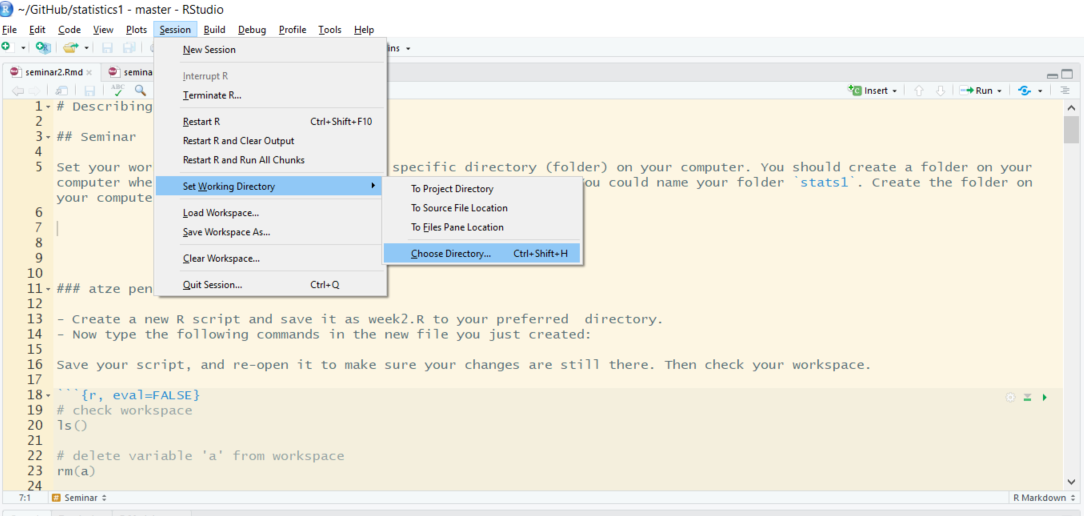
\includegraphics{./img/setwdir.png}
\caption{}
\end{figure}

Create a new R script and save it as week2.R to your \texttt{stats1}
directory. Now type the following commands in the new file you just
created:

\begin{Shaded}
\begin{Highlighting}[]
\CommentTok{# Create a numeric and a character variable}
\NormalTok{a <-}\StringTok{ }\DecValTok{5} \CommentTok{# numeric}
\NormalTok{a <-}\StringTok{ "five"} \CommentTok{# character}
\end{Highlighting}
\end{Shaded}

Save your script, and re-open it to make sure your changes are still
there. Then check your workspace.

\begin{Shaded}
\begin{Highlighting}[]
\CommentTok{# check workspace}
\KeywordTok{ls}\NormalTok{()}

\CommentTok{# delete variable 'a' from workspace}
\KeywordTok{rm}\NormalTok{(a)}

\CommentTok{# delete everything from workspace}
\KeywordTok{rm}\NormalTok{( }\DataTypeTok{list =} \KeywordTok{ls}\NormalTok{() )}

\CommentTok{# to clear console window press Crtl+l on Win or Command+l on Mac}
\end{Highlighting}
\end{Shaded}

\subsubsection{vectors and subsetting}\label{vectors-and-subsetting}

Last week we have already worked with vectors. We created a sequence for
example. This week, we learn about subsetting (accessing specific
elements of our vector).

We create a vector using the \texttt{c()} function, where c stands for
collect.

\begin{Shaded}
\begin{Highlighting}[]
\CommentTok{# Create a vector}
\NormalTok{my.vector <-}\StringTok{ }\KeywordTok{c}\NormalTok{(}\DecValTok{10}\NormalTok{,}\DecValTok{7}\NormalTok{,}\DecValTok{99}\NormalTok{,}\DecValTok{34}\NormalTok{,}\DecValTok{0}\NormalTok{,}\DecValTok{5}\NormalTok{) }\CommentTok{# a vector}
\NormalTok{my.vector}
\end{Highlighting}
\end{Shaded}

\begin{verbatim}
[1] 10  7 99 34  0  5
\end{verbatim}

Let's see how many elements our vector contains using the
\texttt{length()} function.

\begin{Shaded}
\begin{Highlighting}[]
\KeywordTok{length}\NormalTok{(my.vector) }\CommentTok{# how many elements?}
\end{Highlighting}
\end{Shaded}

\begin{verbatim}
[1] 6
\end{verbatim}

Next, we access the first element in our vector. We use square brackets
to access a specific element. The number in the square brackets is the
vector element that we access

\begin{Shaded}
\begin{Highlighting}[]
\CommentTok{# subsetting}
\NormalTok{my.vector[}\DecValTok{1}\NormalTok{] }\CommentTok{# 1st vector element}
\end{Highlighting}
\end{Shaded}

\begin{verbatim}
[1] 10
\end{verbatim}

To access all elements except the first element, we use the \texttt{-}
operator.

\begin{Shaded}
\begin{Highlighting}[]
\NormalTok{my.vector[}\OperatorTok{-}\DecValTok{1}\NormalTok{] }\CommentTok{# all elements but the 1st}
\end{Highlighting}
\end{Shaded}

\begin{verbatim}
[1]  7 99 34  0  5
\end{verbatim}

We can access elements 2 to 4 by using the colon.

\begin{Shaded}
\begin{Highlighting}[]
\NormalTok{my.vector[}\DecValTok{2}\OperatorTok{:}\DecValTok{4}\NormalTok{] }\CommentTok{# the 2nd to the 4th elements}
\end{Highlighting}
\end{Shaded}

\begin{verbatim}
[1]  7 99 34
\end{verbatim}

We can access two specific non-adjacent elements, by using the collect
function \texttt{c()}.

\begin{Shaded}
\begin{Highlighting}[]
\NormalTok{my.vector[}\KeywordTok{c}\NormalTok{(}\DecValTok{2}\NormalTok{,}\DecValTok{5}\NormalTok{)] }\CommentTok{# 2nd and 5th element}
\end{Highlighting}
\end{Shaded}

\begin{verbatim}
[1] 7 0
\end{verbatim}

No, we combine the \texttt{length()} function with the square brackets
to access the last element in our vector.

\begin{Shaded}
\begin{Highlighting}[]
\NormalTok{my.vector[}\KeywordTok{length}\NormalTok{(my.vector)] }\CommentTok{# the last element}
\end{Highlighting}
\end{Shaded}

\begin{verbatim}
[1] 5
\end{verbatim}

\subsubsection{data frames}\label{data-frames}

A data frame is an object that holds data in a tabular format similar to
how spreadsheets work. Variables are generally kept in columns and
observations are in rows.

Before we work with ready-made data, we create a small dataset
ourselves. It contains the populations of the sixteen German states. We
start with a vector that contains the names of those states. We call the
variable \emph{state}. Our variable shall contain text instead of
numbers. In R jargon, this is a character variable, sometimes referred
to as a string. Using quotes, we indicate that the variable type is
character. We use the \texttt{c()} function to create the vector.

\begin{Shaded}
\begin{Highlighting}[]
\CommentTok{# create a character vector containing state names}
\NormalTok{state <-}\StringTok{ }\KeywordTok{c}\NormalTok{(}
  \StringTok{"North Rhine-Westphalia"}\NormalTok{,}
  \StringTok{"Bavaria"}\NormalTok{,}
  \StringTok{"Baden-Wurttemberg"}\NormalTok{,}
  \StringTok{"Lower Saxony"}\NormalTok{,}
  \StringTok{"Hesse"}\NormalTok{,}
  \StringTok{"Saxony"}\NormalTok{,}
  \StringTok{"Rhineland-Palatinate"}\NormalTok{,}
  \StringTok{"Berlin"}\NormalTok{,}
  \StringTok{"Schleswig-Holstein"}\NormalTok{,}
  \StringTok{"Brandenburg"}\NormalTok{,}
  \StringTok{"Saxony-Anhalt"}\NormalTok{,}
  \StringTok{"Thuringia"}\NormalTok{,}
  \StringTok{"Hamburg"}\NormalTok{,}
  \StringTok{"Mecklenburg-Vorpommern"}\NormalTok{,}
  \StringTok{"Saarland"}\NormalTok{,}
  \StringTok{"Bremen"}
\NormalTok{  )}
\end{Highlighting}
\end{Shaded}

Now, we create a second variable for the populations. This is a numeric
vector, so we do not use the quotes.

\begin{Shaded}
\begin{Highlighting}[]
\NormalTok{population <-}\StringTok{ }\KeywordTok{c}\NormalTok{(}
  \DecValTok{17865516}\NormalTok{,}
  \DecValTok{12843514}\NormalTok{,}
  \DecValTok{10879618}\NormalTok{,}
  \DecValTok{7926599}\NormalTok{,}
  \DecValTok{6176172}\NormalTok{,}
  \DecValTok{4084851}\NormalTok{,}
  \DecValTok{4052803}\NormalTok{,}
  \DecValTok{3670622}\NormalTok{,}
  \DecValTok{2858714}\NormalTok{,}
  \DecValTok{2484826}\NormalTok{,}
  \DecValTok{2245470}\NormalTok{,}
  \DecValTok{2170714}\NormalTok{,}
  \DecValTok{1787408}\NormalTok{,}
  \DecValTok{1612362}\NormalTok{,}
  \DecValTok{995597}\NormalTok{,}
  \DecValTok{671489}
\NormalTok{)}
\end{Highlighting}
\end{Shaded}

Now with both vectors created, we combine them into a dataframe. We put
our vectors in and give them names. In this case the variable names in
the dataset correspond to our vector names. The name goes in front of
the equal sign and the vector object name, after.

\begin{Shaded}
\begin{Highlighting}[]
\NormalTok{popdata <-}\StringTok{ }\KeywordTok{data.frame}\NormalTok{( }
  \DataTypeTok{state =}\NormalTok{ state,}
  \DataTypeTok{population =}\NormalTok{ population}
\NormalTok{  )}
\end{Highlighting}
\end{Shaded}

You should see the new data frame object in your global environment
window. You can view the dataset in the spreadsheet form that we are all
used to by clicking on the oject name.

We can see the names of variables in our dataset with the names function

\begin{Shaded}
\begin{Highlighting}[]
\KeywordTok{names}\NormalTok{(popdata)}
\end{Highlighting}
\end{Shaded}

\begin{verbatim}
[1] "state"      "population"
\end{verbatim}

Let's check the variable types in our data using the \texttt{str()}
function.

\begin{Shaded}
\begin{Highlighting}[]
\KeywordTok{str}\NormalTok{(popdata)}
\end{Highlighting}
\end{Shaded}

\begin{verbatim}
'data.frame':   16 obs. of  2 variables:
 $ state     : Factor w/ 16 levels "Baden-Wurttemberg",..: 10 2 1 8 7 13 11 3 15 4 ...
 $ population: num  17865516 12843514 10879618 7926599 6176172 ...
\end{verbatim}

The variable \emph{state} is a factor variable. R has turned the
character variable into a categorical variable automatically. The
variable \emph{population} is numeric. These variable types differ. We
can calculate with numeric variables only.

Often we want to access certain observations (rows) or certain columns
(variables) or a combination of the two without looking at the entire
dataset all at once. We can use square brackets to subset data frames.
In square brackets we put a row and a column coordinate separated by a
comma. The row coordinate goes first and the column coordinate second.
So \texttt{popdata{[}10,\ 2{]}} returns the 10th row and second column
of the data frame. If we leave the column coordinate empty this means we
would like all columns. So, \texttt{popdata{[}10,{]}} returns the 10th
row of the dataset. If we leave the row coordinate empty, R returns the
entire column. \texttt{popdata{[},2{]}} returns the second column of the
dataset.

We can look at the first five rows of a dataset to get a better
understanding of it with the colon in brackets like so:
\texttt{popdata{[}1:5,{]}}. We could display the second and fifth
columns of the dataset by using the \texttt{c()} function in brackets
like so: \texttt{popdata{[},\ c(2,5){]}}.

It's your turn. Display all columns of the popdata dataset and show rows
10 to 15. Next display all columns of the dataset and rows 4 and 7.

\begin{Shaded}
\begin{Highlighting}[]
\NormalTok{popdata[}\DecValTok{10}\OperatorTok{:}\DecValTok{15}\NormalTok{, ] }\CommentTok{# elements in 10th to 15th row, all columns}
\end{Highlighting}
\end{Shaded}

\begin{verbatim}
                    state population
10            Brandenburg    2484826
11          Saxony-Anhalt    2245470
12              Thuringia    2170714
13                Hamburg    1787408
14 Mecklenburg-Vorpommern    1612362
15               Saarland     995597
\end{verbatim}

\begin{Shaded}
\begin{Highlighting}[]
\NormalTok{popdata[}\KeywordTok{c}\NormalTok{(}\DecValTok{4}\NormalTok{, }\DecValTok{7}\NormalTok{), ] }\CommentTok{# elements in 4th and 7th row, all column}
\end{Highlighting}
\end{Shaded}

\begin{verbatim}
                 state population
4         Lower Saxony    7926599
7 Rhineland-Palatinate    4052803
\end{verbatim}

In order to access individual columns of a data frame we can also use
the dollar sign \texttt{\$}. For example, let's see how to access the
\texttt{population} column.

\begin{Shaded}
\begin{Highlighting}[]
\NormalTok{popdata}\OperatorTok{$}\NormalTok{population}
\end{Highlighting}
\end{Shaded}

\begin{verbatim}
 [1] 17865516 12843514 10879618  7926599  6176172  4084851  4052803
 [8]  3670622  2858714  2484826  2245470  2170714  1787408  1612362
[15]   995597   671489
\end{verbatim}

Now, access the state column.

\begin{Shaded}
\begin{Highlighting}[]
\NormalTok{popdata}\OperatorTok{$}\NormalTok{state}
\end{Highlighting}
\end{Shaded}

\begin{verbatim}
 [1] North Rhine-Westphalia Bavaria                Baden-Wurttemberg     
 [4] Lower Saxony           Hesse                  Saxony                
 [7] Rhineland-Palatinate   Berlin                 Schleswig-Holstein    
[10] Brandenburg            Saxony-Anhalt          Thuringia             
[13] Hamburg                Mecklenburg-Vorpommern Saarland              
[16] Bremen                
16 Levels: Baden-Wurttemberg Bavaria Berlin Brandenburg Bremen ... Thuringia
\end{verbatim}

\subsubsection{Loading data}\label{loading-data}

Before you load the dataset into R, you first download it and save it
locally in your \texttt{Stats1} folder. Download the data
\href{http://philippbroniecki.github.io/ML2017.io/data/BSAS_manip.RData}{here}.

We often load existing data sets into R for analysis. Data come in many
different file formats such as \texttt{.csv}, \texttt{.tab},
\texttt{.dta}, etc. Today we will load a dataset which is stored in R's
native file format: \texttt{.RData}. The function to load data from this
file format is called: \texttt{load()}. If you managed to set your
working directory correctly just now
(\texttt{setwd("\textasciitilde{}/Stats1"})), then you should just be
able to run the line of code below.

We load the dataset with the \texttt{load()} function:

\begin{Shaded}
\begin{Highlighting}[]
\CommentTok{# load perception of non-western foreigners data}
\KeywordTok{load}\NormalTok{(}\StringTok{"BSAS_manip.RData"}\NormalTok{)}
\end{Highlighting}
\end{Shaded}

The non-western foreingers data is about the subjective perception of
immigrants from non-western countries. The perception of immigrants from
a context that is not similar to the one's own ,is often used as a proxy
for racism. Whether this is a fair measure or not is debatable but let's
examine the data from a survey carried out in Britain.

Let's check the codebook of our data.

\begin{tabular}{l|l}
\hline
Variable & Description\\
\hline
IMMBRIT & Out of every 100 people in Britain, how many do you think are immigrants from non-western countries?\\
\hline
over.estimate & 1 if estimate is higher than 10.7\%.\\
\hline
RSex & 1 = male, 2 = female\\
\hline
RAge & Age of respondent\\
\hline
Househld & Number of people living in respondent's household\\
\hline
party identification & 1 = Conservatives, 2 = Labour, 3 = SNP, 4 = Greens, 5 = Ukip, 6 = BNP, 7 = other\\
\hline
paper & Do you normally read any daily morning newspaper 3+ times/week?\\
\hline
WWWhourspW & How many hours WWW per week?\\
\hline
religious & Do you regard yourself as belonging to any particular religion?\\
\hline
employMonths & How many mnths w. present employer?\\
\hline
urban & Population density, 4 categories (highest density is 4, lowest is 1)\\
\hline
health.good & How is your health in general for someone of your age? (0: bad, 1: fair, 2: fairly good, 3: good)\\
\hline
HHInc & Income bands for household, high number = high HH income\\
\hline
\end{tabular}

We can look at the variable names in our data with the
\href{http://bit.ly/R_names}{\texttt{names()}} function.

The \href{http://bit.ly/R_dim}{\texttt{dim()}} function can be used to
find out the dimensions of the dataset (dimension 1 = rows, dimension 2
= columns).

\begin{Shaded}
\begin{Highlighting}[]
\KeywordTok{dim}\NormalTok{(data2)}
\end{Highlighting}
\end{Shaded}

\begin{verbatim}
[1] 1049   19
\end{verbatim}

So, the \href{http://bit.ly/R_dim}{\texttt{dim()}} function tells us
that we have data from 1049 respondents with 19 variables for each
respondent.

Let's take a quick peek at the first 10 observations to see what the
dataset looks like. By default the
\href{http://bit.ly/R_head}{\texttt{head()}} function returns the first
6 rows, but let's tell it to return the first 10 rows instead.

\begin{Shaded}
\begin{Highlighting}[]
\KeywordTok{head}\NormalTok{(data2, }\DataTypeTok{n =} \DecValTok{10}\NormalTok{)}
\end{Highlighting}
\end{Shaded}

\begin{verbatim}
   IMMBRIT over.estimate RSex RAge Househld Cons Lab SNP Ukip BNP GP
1        1             0    1   50        2    0   1   0    0   0  0
2       50             1    2   18        3    0   0   0    0   0  0
3       50             1    2   60        1    0   0   0    0   0  0
4       15             1    2   77        2    0   0   0    0   0  0
5       20             1    2   67        1    0   0   0    0   0  0
6       30             1    1   30        4    0   0   0    0   0  0
7       60             1    2   56        2    0   0   1    0   0  0
8        7             0    1   49        1    0   0   0    0   0  0
9       30             1    1   40        4    0   0   1    0   0  0
10       2             0    1   61        3    1   0   0    0   0  0
   party.other paper WWWhourspW religious employMonths urban health.good
1            0     0          1         0           72     4           1
2            1     0          4         0           72     4           2
3            1     0          1         0          456     3           3
4            1     1          2         1           72     1           3
5            1     0          1         1           72     3           3
6            1     1         14         0           72     1           2
7            0     0          5         1          180     1           2
8            1     1          8         0          156     4           2
9            0     0          3         1          264     2           2
10           0     1          0         1           72     1           3
   HHInc
1     13
2      3
3      9
4      8
5      9
6      9
7     13
8     14
9     11
10     8
\end{verbatim}

\subsubsection{Plots}\label{plots}

We can visualize the data with the help of a boxplot, so let's see how
the perception of the number of immigrants is distributed.

\begin{Shaded}
\begin{Highlighting}[]
\CommentTok{# how good are we at guessing immigration}
\KeywordTok{boxplot}\NormalTok{(}
\NormalTok{  data2}\OperatorTok{$}\NormalTok{IMMBRIT, }
  \DataTypeTok{main =} \StringTok{"Perception of Immigration from Non-Western Countries"}\NormalTok{,}
  \DataTypeTok{ylab =} \StringTok{"Subjective number of immigrants per 100 British"}\NormalTok{, }
  \DataTypeTok{frame.plot =} \OtherTok{FALSE}\NormalTok{, }\DataTypeTok{col =} \StringTok{"darkgray"}
\NormalTok{  )}
\end{Highlighting}
\end{Shaded}

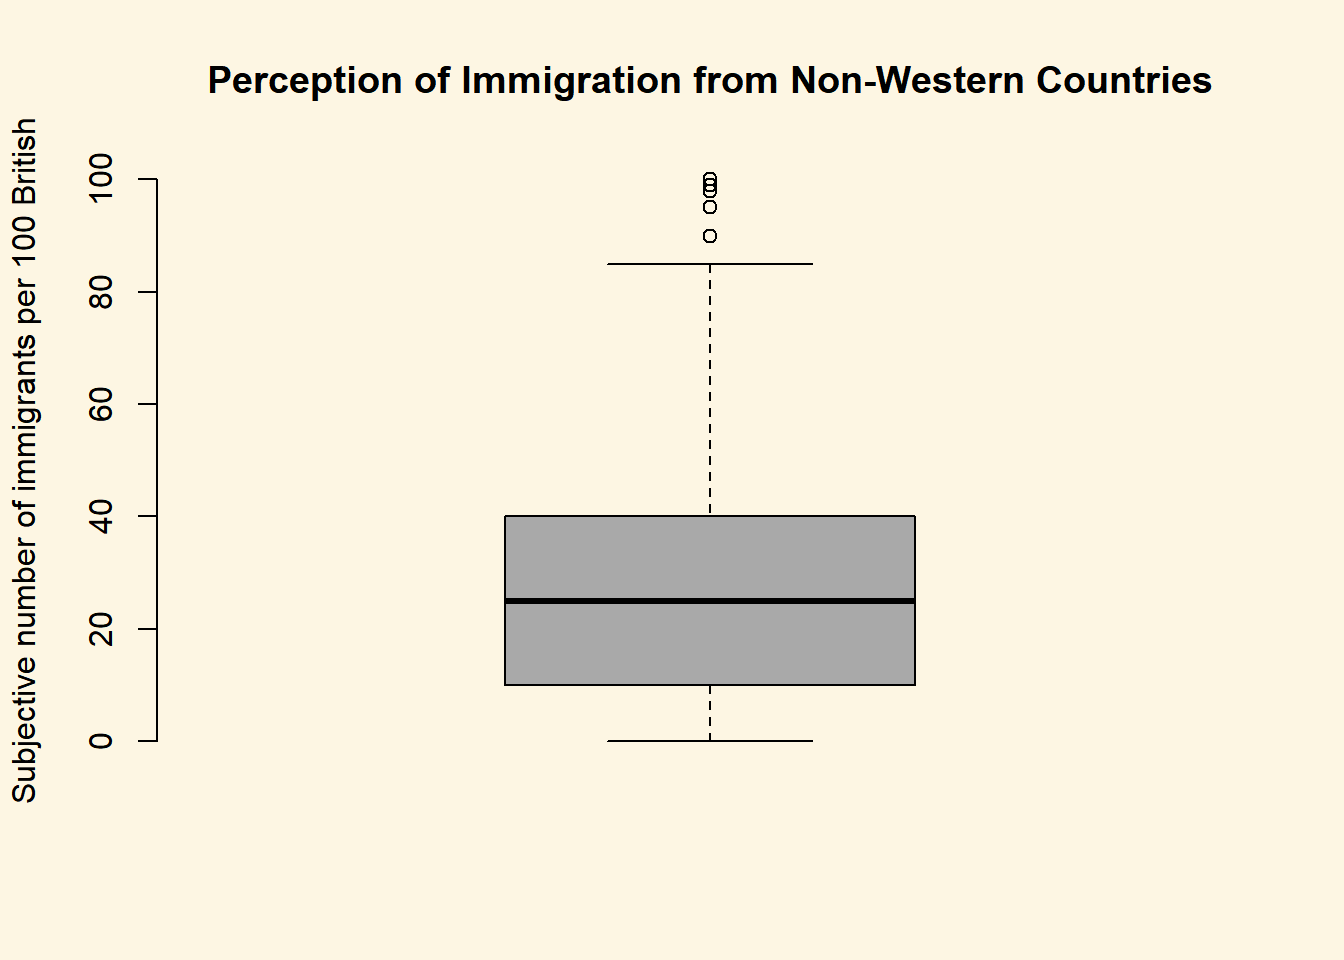
\includegraphics{statistics1_files/figure-latex/unnamed-chunk-72-1.pdf}

Notice how the lower whisker is much shorter than the upper one. The
distribution is right skewed. The right tail (higher values) is a lot
longer. We can see this beter using a density plot. We combine R's
\texttt{denisty()} function with the \texttt{plot()} function.

\begin{Shaded}
\begin{Highlighting}[]
\KeywordTok{plot}\NormalTok{(}
  \KeywordTok{density}\NormalTok{(data2}\OperatorTok{$}\NormalTok{IMMBRIT),}
  \DataTypeTok{bty =} \StringTok{"n"}\NormalTok{,}
  \DataTypeTok{main =} \StringTok{"Perception of Immigration from Non-Western Countries"}\NormalTok{,}
  \DataTypeTok{xlab =} \StringTok{"Subjective number of immigrants per 100 British"}
\NormalTok{  )}
\end{Highlighting}
\end{Shaded}

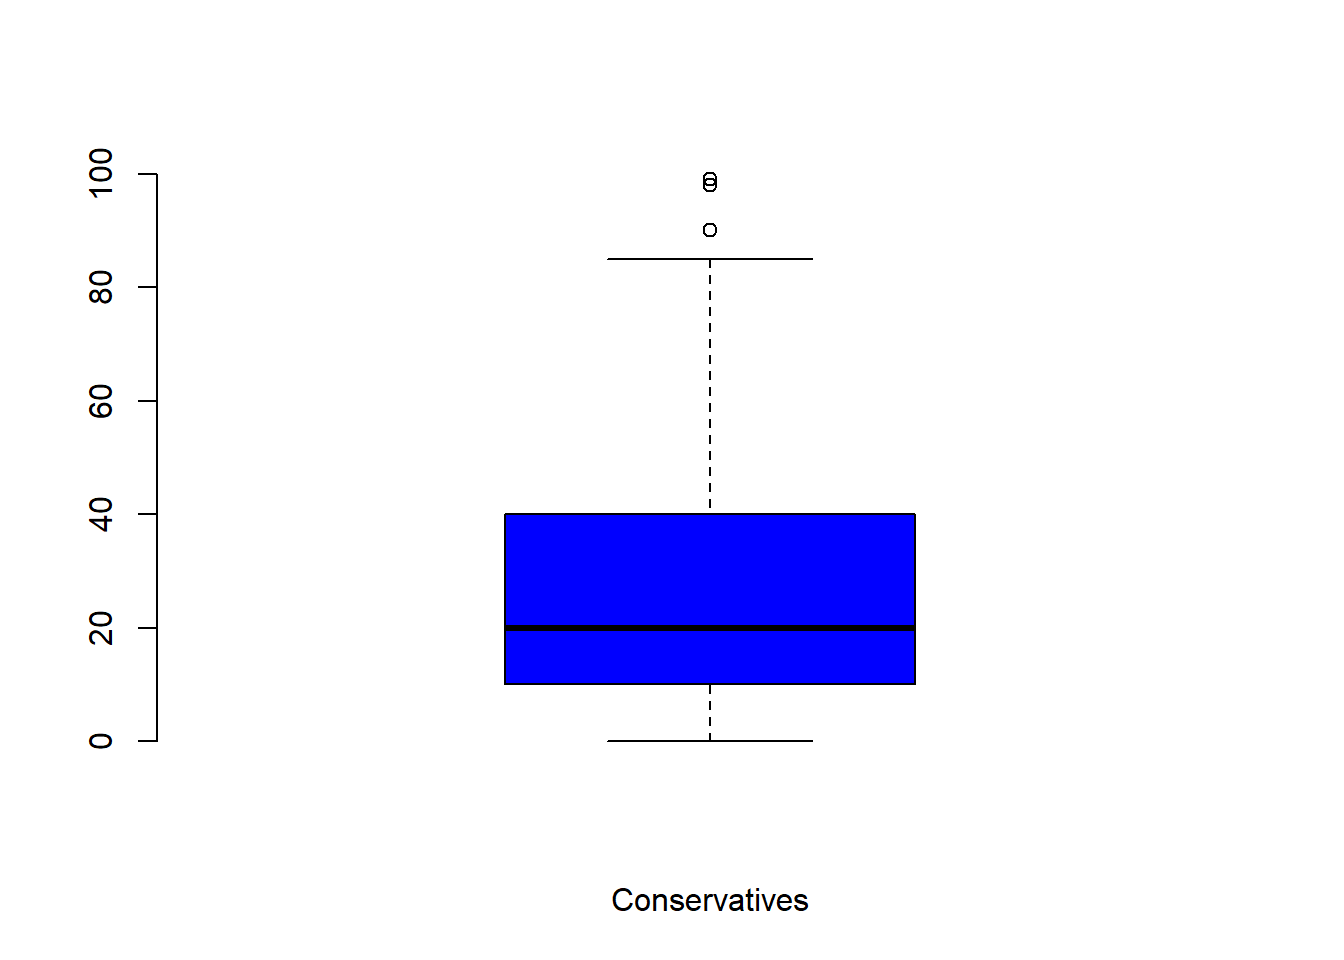
\includegraphics{statistics1_files/figure-latex/unnamed-chunk-73-1.pdf}

We can also plot histograms using the \texttt{hist()} function.

\begin{Shaded}
\begin{Highlighting}[]
\CommentTok{# histogram}
\KeywordTok{hist}\NormalTok{( data2}\OperatorTok{$}\NormalTok{employMonths, }\DataTypeTok{main =} \StringTok{"histogram"}\NormalTok{)}
\end{Highlighting}
\end{Shaded}

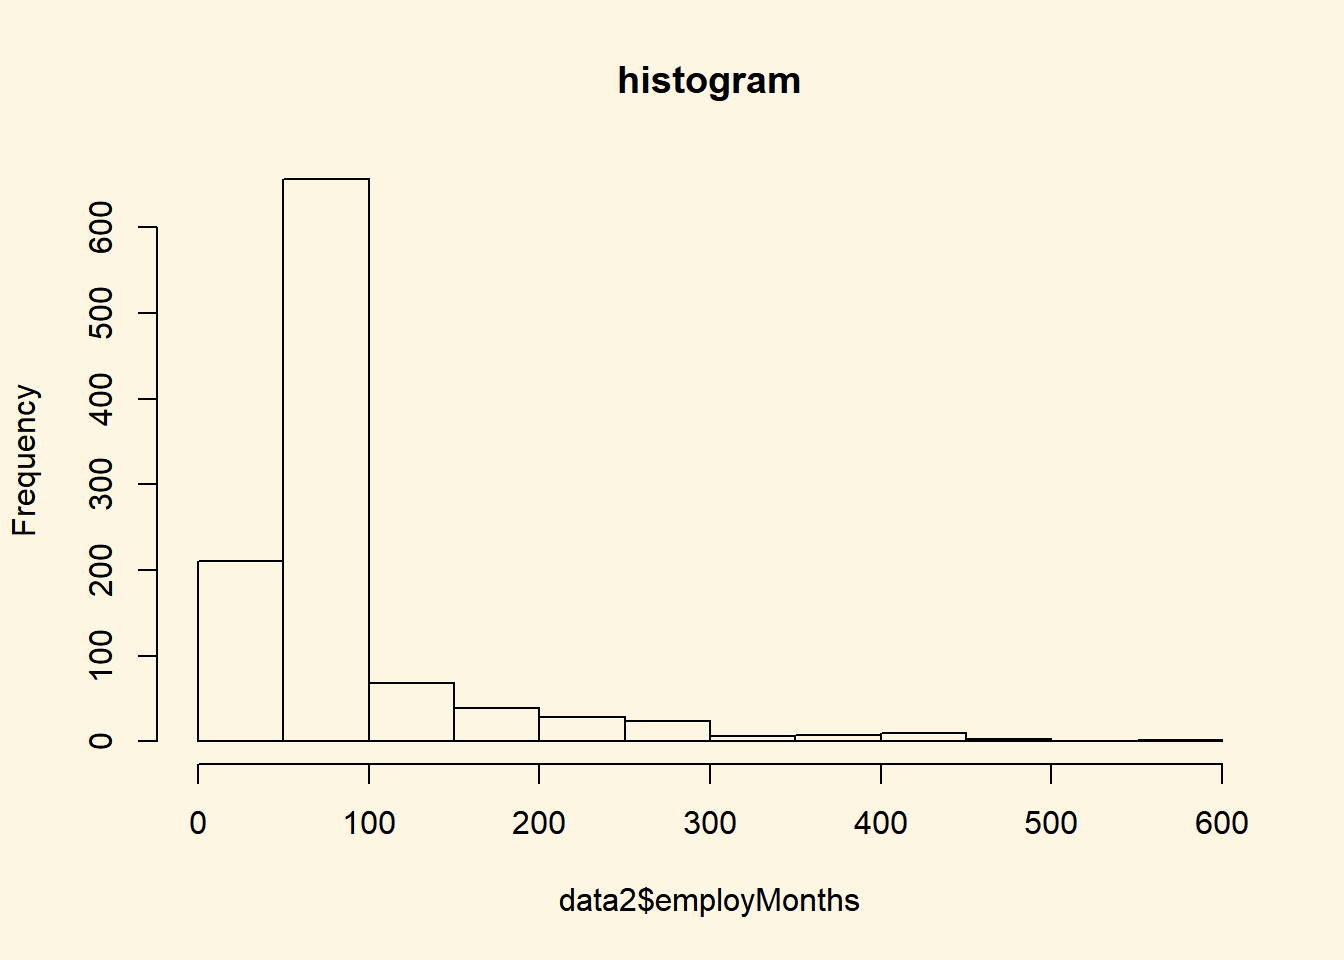
\includegraphics{statistics1_files/figure-latex/unnamed-chunk-74-1.pdf}

It is plausible that perception of immigration from Non-Western
countries is related to party affiliation. In our dataset, we have a
some party affiliation dummies (binary variables). We can use square
brackets to subset our data such that we produce a boxplot only for
members of the Conservative Party. We have a look at the variable
\emph{Cons} using the \texttt{table()} function first.

\begin{Shaded}
\begin{Highlighting}[]
\KeywordTok{table}\NormalTok{(data2}\OperatorTok{$}\NormalTok{Cons)}
\end{Highlighting}
\end{Shaded}

\begin{verbatim}

  0   1 
765 284 
\end{verbatim}

In our data, 284 respondents associate with the Conservative party and
765 do not. We create a boxplot of \emph{IMMBRIT} but only for members
of the Conservative Party. We do so by using the square brackets to
subset our data.

\begin{Shaded}
\begin{Highlighting}[]
\CommentTok{# boxplot of immbrit for those observations where Cons is 1}
\KeywordTok{boxplot}\NormalTok{(}
\NormalTok{  data2}\OperatorTok{$}\NormalTok{IMMBRIT[data2}\OperatorTok{$}\NormalTok{Cons}\OperatorTok{==}\DecValTok{1}\NormalTok{],}
  \DataTypeTok{frame.plot =} \OtherTok{FALSE}\NormalTok{,}
  \DataTypeTok{xlab =} \StringTok{"Conservatives"}\NormalTok{,}
  \DataTypeTok{col =} \StringTok{"blue"}
\NormalTok{  )}
\end{Highlighting}
\end{Shaded}

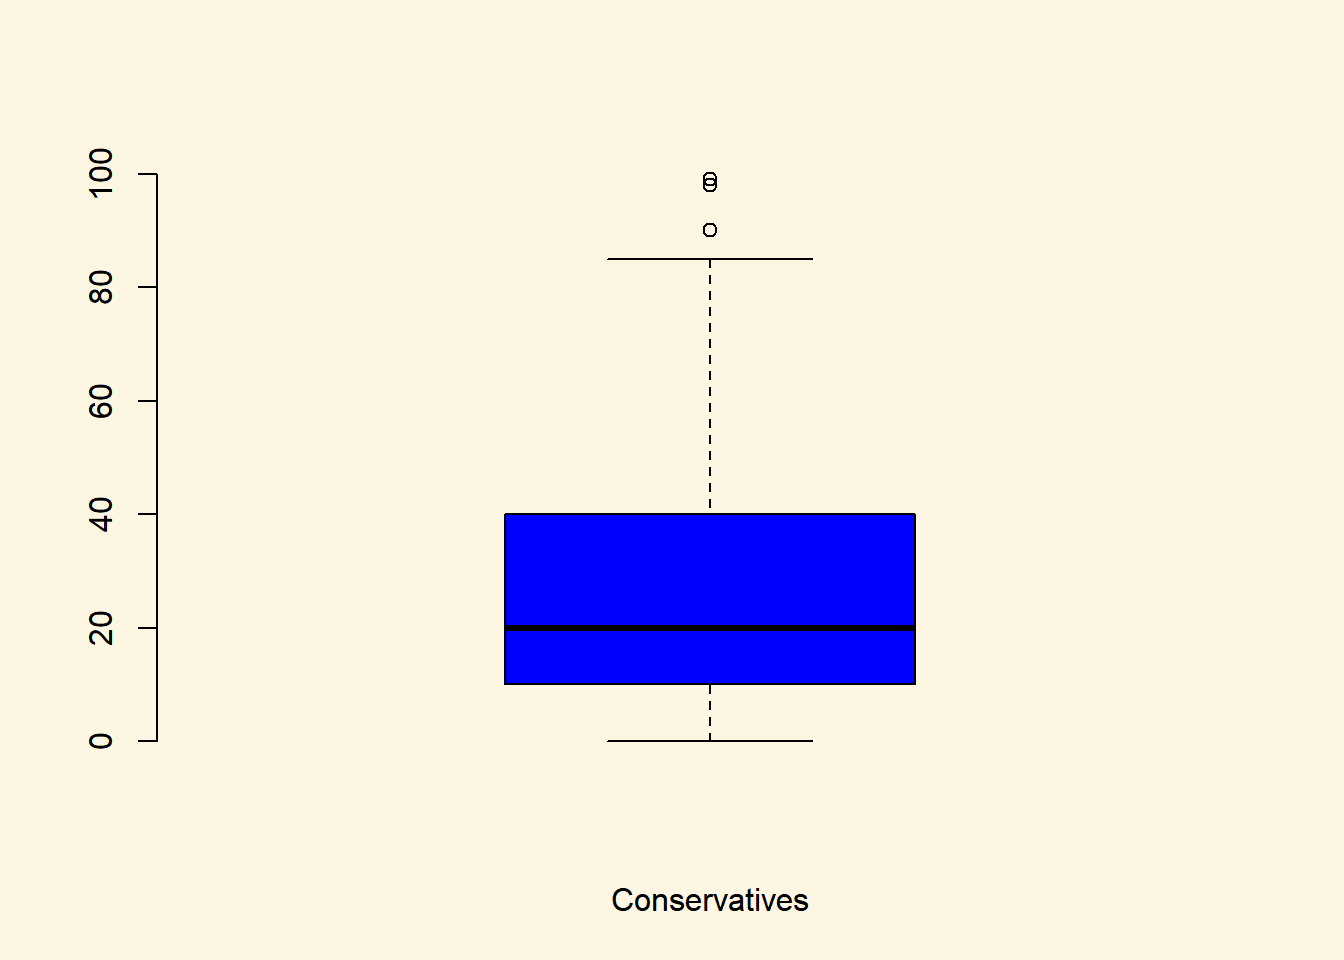
\includegraphics{statistics1_files/figure-latex/unnamed-chunk-76-1.pdf}

We would now like to compare the distribution of the perception fo
Conservatives to the distribution among Labour respondents. We can
subset the data just like we did for the Conservative Party. In addtion,
we want to plot the two plots next to each other, i.e., they should be
in the same plot. We can achieve this with the \texttt{par()} function
and the \texttt{mfrow} argument. This will spilt the plot window into
rows and columns. We want 2 columns to plot 2 boxplots next to each
other.

\begin{Shaded}
\begin{Highlighting}[]
\CommentTok{# split plot window into 1 row and 2 columns}
\KeywordTok{par}\NormalTok{(}\DataTypeTok{mfrow =} \KeywordTok{c}\NormalTok{(}\DecValTok{1}\NormalTok{,}\DecValTok{2}\NormalTok{))}

\CommentTok{# plot 1}
\KeywordTok{boxplot}\NormalTok{(}
\NormalTok{  data2}\OperatorTok{$}\NormalTok{IMMBRIT[data2}\OperatorTok{$}\NormalTok{Cons}\OperatorTok{==}\DecValTok{1}\NormalTok{],}
  \DataTypeTok{frame.plot =} \OtherTok{FALSE}\NormalTok{,}
  \DataTypeTok{xlab =} \StringTok{"Conservatives"}\NormalTok{,}
  \DataTypeTok{col =} \StringTok{"blue"}
\NormalTok{  )}

\CommentTok{# plot 2}
\KeywordTok{boxplot}\NormalTok{(}
\NormalTok{  data2}\OperatorTok{$}\NormalTok{IMMBRIT[data2}\OperatorTok{$}\NormalTok{Lab}\OperatorTok{==}\DecValTok{1}\NormalTok{],}
  \DataTypeTok{frame.plot =} \OtherTok{FALSE}\NormalTok{,}
  \DataTypeTok{xlab =} \StringTok{"Labour"}\NormalTok{,}
  \DataTypeTok{col =} \StringTok{"red"}
\NormalTok{  )}
\end{Highlighting}
\end{Shaded}

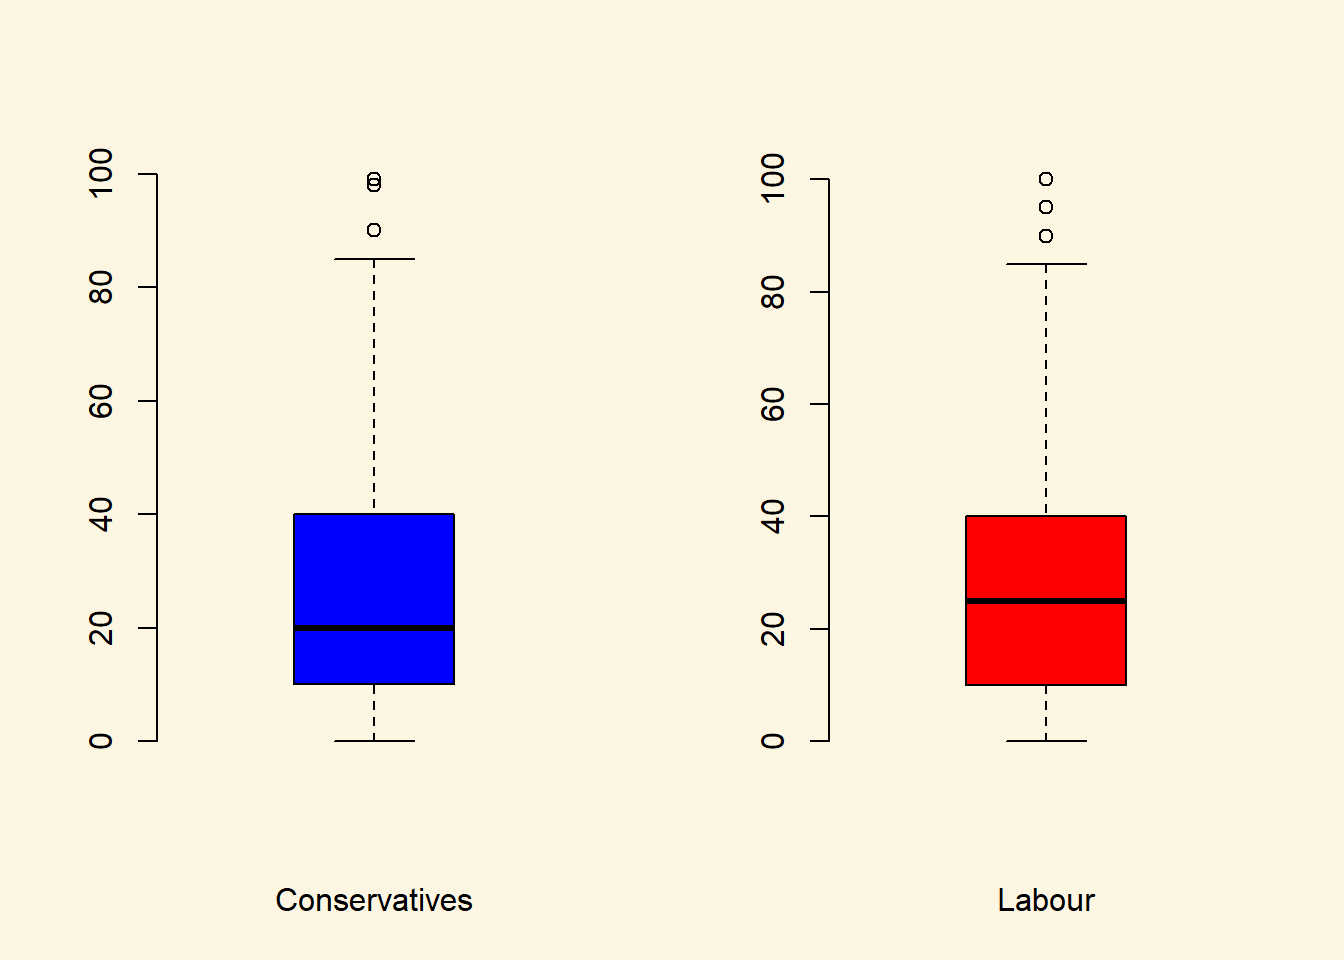
\includegraphics{statistics1_files/figure-latex/unnamed-chunk-77-1.pdf}

It is very hard to spot differences. The distributions are similar. The
median for Labour respondents is larger which mean that the central
Labour respondent over-estimates immigration more than the central
Conservative respondent.

You can play around with the non-western foreigners data on your own
time. We now turn to a dataset that is integrated in R already. It is
called \texttt{longley}. Use the \texttt{help()} function to see what
this dataset is about.

\begin{Shaded}
\begin{Highlighting}[]
\KeywordTok{help}\NormalTok{(longley)}
\end{Highlighting}
\end{Shaded}

Let's create a scatterplot with the \texttt{Year} variable on the x-axis
and \texttt{Employed} on the y-axis.

\begin{Shaded}
\begin{Highlighting}[]
\KeywordTok{plot}\NormalTok{(}\DataTypeTok{x =}\NormalTok{ longley}\OperatorTok{$}\NormalTok{Year, }\CommentTok{# x-axis variable}
     \DataTypeTok{y =}\NormalTok{ longley}\OperatorTok{$}\NormalTok{Employed, }\CommentTok{# y-axis variable}
     \DataTypeTok{bty =} \StringTok{"n"} \CommentTok{# no box around the plot}
\NormalTok{     )}
\end{Highlighting}
\end{Shaded}

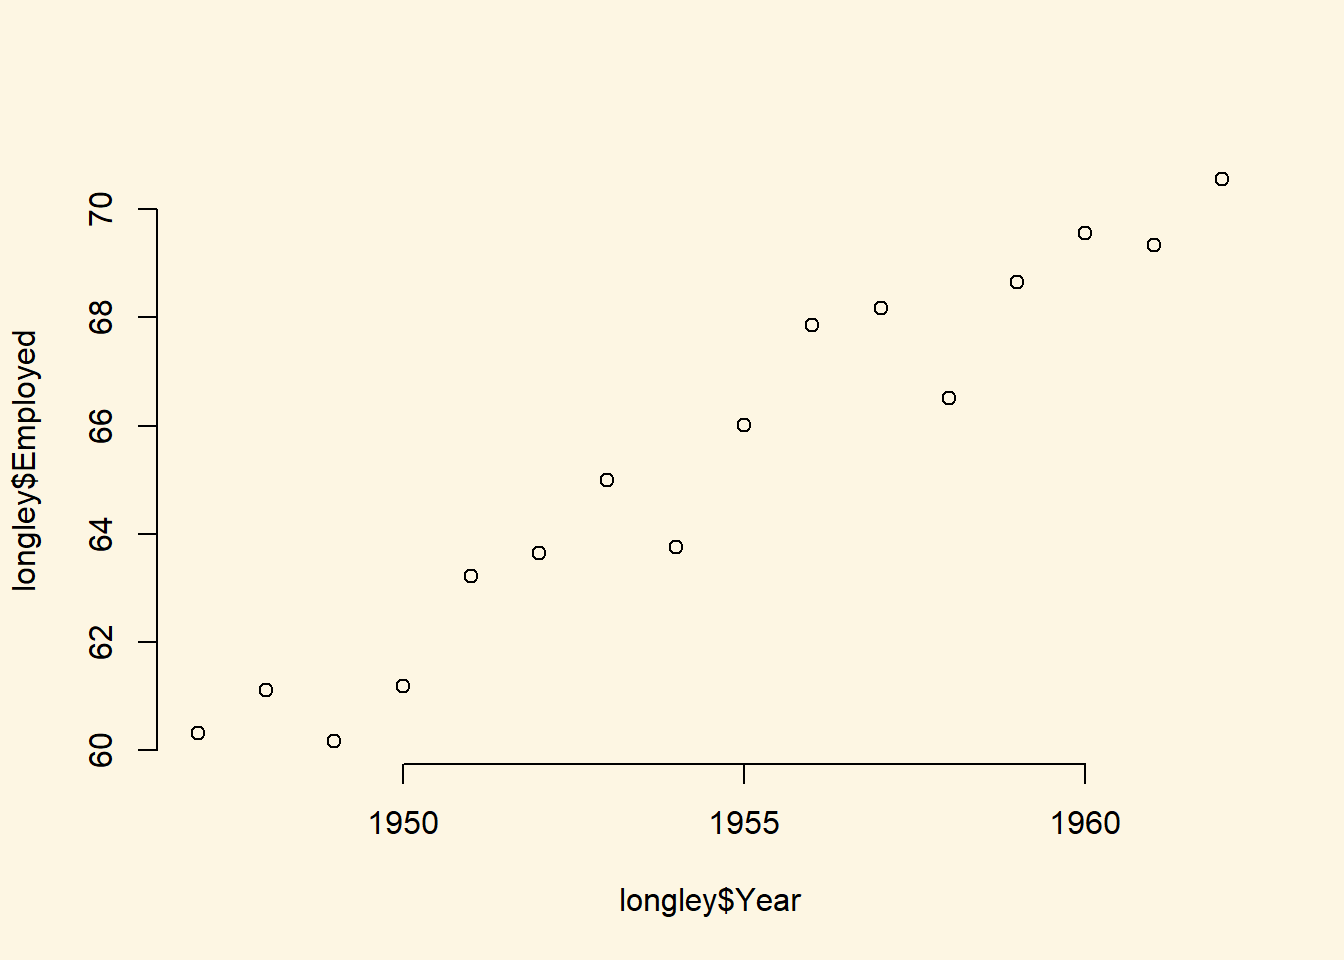
\includegraphics{statistics1_files/figure-latex/unnamed-chunk-80-1.pdf}

To create a line plot instead, we use the same function with one
additional argument \texttt{type\ =\ "l"}.

\begin{Shaded}
\begin{Highlighting}[]
\KeywordTok{plot}\NormalTok{(longley}\OperatorTok{$}\NormalTok{Year, longley}\OperatorTok{$}\NormalTok{Employed, }\DataTypeTok{type =} \StringTok{"l"}\NormalTok{)}
\end{Highlighting}
\end{Shaded}

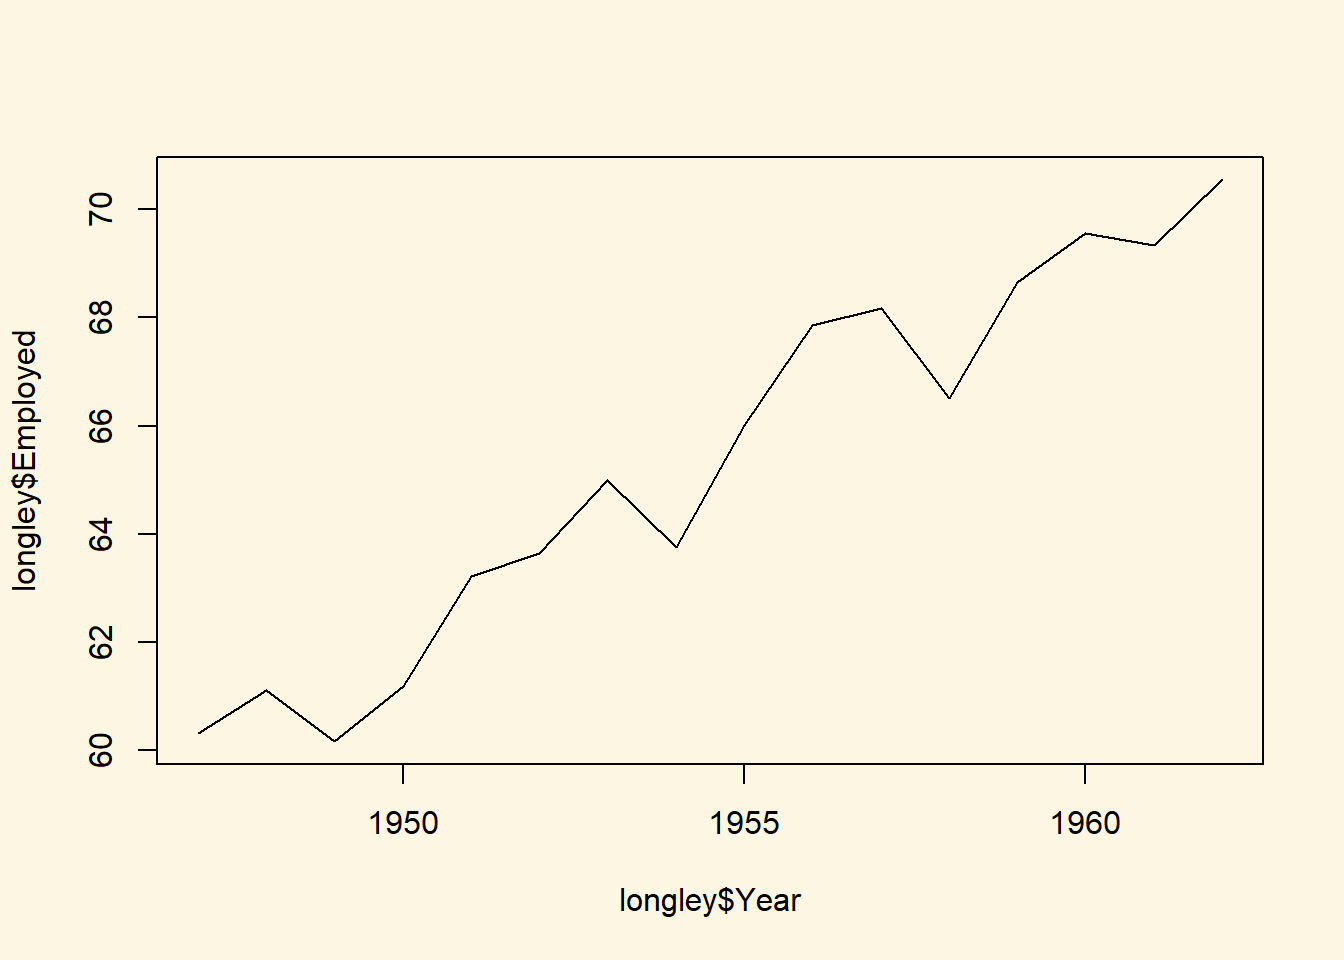
\includegraphics{statistics1_files/figure-latex/unnamed-chunk-81-1.pdf}

Create a plot that includes both points and lines.

\begin{Shaded}
\begin{Highlighting}[]
\KeywordTok{plot}\NormalTok{(longley}\OperatorTok{$}\NormalTok{Year, longley}\OperatorTok{$}\NormalTok{Employed, }\DataTypeTok{type =} \StringTok{"b"}\NormalTok{)}
\end{Highlighting}
\end{Shaded}

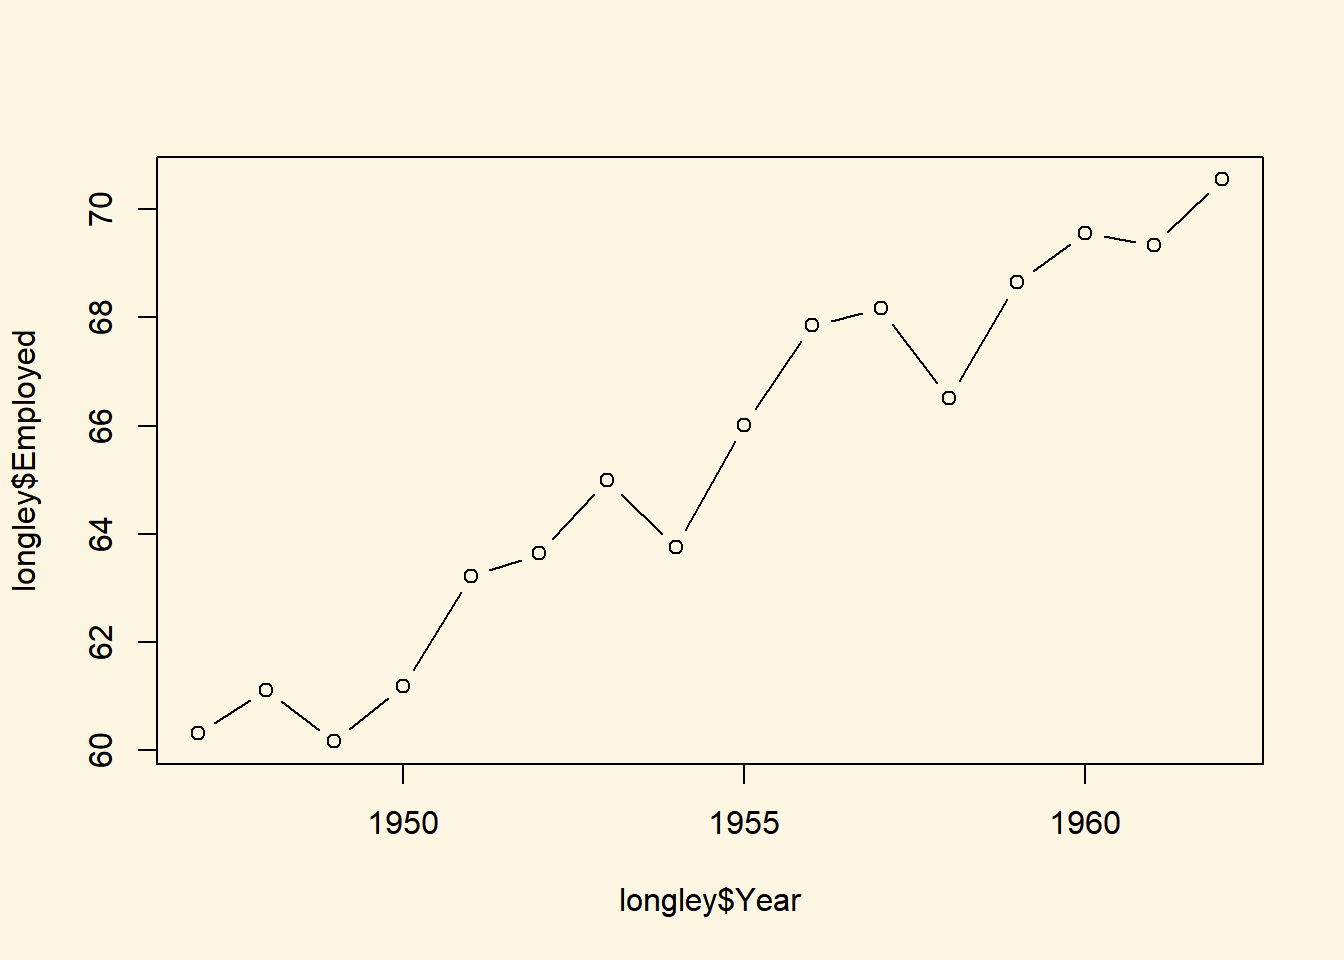
\includegraphics{statistics1_files/figure-latex/unnamed-chunk-82-1.pdf}

\subsubsection{Average Treatment Effect}\label{average-treatment-effect}

In the lecture, we estimated the average treatment effect on a small
example. We will do this again here. Recall, that the average treatment
effect is the difference between two means.

Let's suppose, associating with right-wing parties causes people to
over-estimate the number of non-western foreigners. Our treatment
variable is whether a respondent assoicates with the UK Independence
Party. It is 1 if that is the case and 0 otherwise. Let's inspect the
variable \emph{Ukip}.

\begin{Shaded}
\begin{Highlighting}[]
\KeywordTok{table}\NormalTok{(data2}\OperatorTok{$}\NormalTok{Ukip)}
\end{Highlighting}
\end{Shaded}

\begin{verbatim}

   0    1 
1018   31 
\end{verbatim}

31 respondents identify with Ukip.

The average treatment effect, as we learned, would be the difference
between the mean outcomes for those who received the treament minus the
mean for those who did not reicive the treatment.

We have all the tools to solve the problem. Let's take the mean of the
treated group first.

\begin{Shaded}
\begin{Highlighting}[]
\NormalTok{mean.y.treated <-}\StringTok{ }\KeywordTok{mean}\NormalTok{(data2}\OperatorTok{$}\NormalTok{IMMBRIT[data2}\OperatorTok{$}\NormalTok{Ukip }\OperatorTok{==}\StringTok{ }\DecValTok{1}\NormalTok{])}
\NormalTok{mean.y.treated}
\end{Highlighting}
\end{Shaded}

\begin{verbatim}
[1] 24.29032
\end{verbatim}

The double equal sign \texttt{==} is a logical operator and means ``is
equal to''. R returns true or false depending on whether the respondent
does identify with Ukip or not. The mean of \emph{IMMBRIT} is then
computed only for respondents who accociate with Ukip.

Let's take the mean of the second group, the untreated group.

\begin{Shaded}
\begin{Highlighting}[]
\NormalTok{mean.y.untreated <-}\StringTok{ }\KeywordTok{mean}\NormalTok{(data2}\OperatorTok{$}\NormalTok{IMMBRIT[data2}\OperatorTok{$}\NormalTok{Ukip }\OperatorTok{==}\StringTok{ }\DecValTok{0}\NormalTok{])}
\NormalTok{mean.y.untreated}
\end{Highlighting}
\end{Shaded}

\begin{verbatim}
[1] 29.17485
\end{verbatim}

The treatment effect is the difference in means:

\begin{Shaded}
\begin{Highlighting}[]
\NormalTok{mean.y.treated }\OperatorTok{-}\StringTok{ }\NormalTok{mean.y.untreated}
\end{Highlighting}
\end{Shaded}

\begin{verbatim}
[1] -4.88453
\end{verbatim}

The result is surprising. Ukip members over-estimate the number of
non-western foreigners less members of all other paries. Our claim is
not quite supported by the data. We should be very careful with these
results, however. We used experimental language but our data is
observational. A multitude of confounders could bias our estimate of the
causal effect.

\subsubsection{Exercises}\label{exercises-1}

\begin{enumerate}
\def\labelenumi{\arabic{enumi}.}
\tightlist
\item
  Create a script and call it assignment02. Save your script.
\item
  Use the \texttt{names()} function to display the variable names of the
  \texttt{longley} dataset.
\item
  Use square brackets to access the 4th column of the dataset.
\item
  Use the dollar sign to access the 4th column of the dataset.
\item
  Access the two cells from row 4 and column 1 and row 6 and column 3.
\item
  Using the \texttt{longley} data produce a line plot with GNP on the
  y-axis and population on the x-axis.
\item
  Use the help function to find out how to label the y-axis ``wealth''
  and the x-axis ``population''.
\item
  Create a boxplot showing the distribution of \emph{IMMBRIT} by each
  party in the data and plot these in one plot next to each other.
\item
  Is there a difference between women and men in terms of their
  subjective estimation of foreingers?
\item
  What is the difference between women and men?
\item
  Could you form a hypothesis out of the relationship that you see if
  any exists?
\item
  Save your script, which should now include the answers to all the
  exercises.
\item
  Source your script, i.e.~run the entire script without error message.
  Clean your script if you get error messages.
\end{enumerate}

\subsection{Solutions}\label{solutions-1}

\subsubsection{Exercise 2}\label{exercise-2}

Use the \texttt{names()} function to display the variable names of the
\texttt{longley} dataset.

\begin{Shaded}
\begin{Highlighting}[]
\KeywordTok{names}\NormalTok{(longley)}
\end{Highlighting}
\end{Shaded}

\begin{verbatim}
[1] "GNP.deflator" "GNP"          "Unemployed"   "Armed.Forces"
[5] "Population"   "Year"         "Employed"    
\end{verbatim}

\subsubsection{Exercise 3}\label{exercise-3-1}

Use square brackets to access the 4th column of the dataset.

\begin{Shaded}
\begin{Highlighting}[]
\NormalTok{longley[, }\DecValTok{4}\NormalTok{]}
\end{Highlighting}
\end{Shaded}

\begin{verbatim}
 [1] 159.0 145.6 161.6 165.0 309.9 359.4 354.7 335.0 304.8 285.7 279.8
[12] 263.7 255.2 251.4 257.2 282.7
\end{verbatim}

\subsubsection{Exercise 4}\label{exercise-4-1}

Use the dollar sign to access the 4th column of the dataset.

\begin{Shaded}
\begin{Highlighting}[]
\NormalTok{longley}\OperatorTok{$}\NormalTok{Armed.Forces}
\end{Highlighting}
\end{Shaded}

\begin{verbatim}
 [1] 159.0 145.6 161.6 165.0 309.9 359.4 354.7 335.0 304.8 285.7 279.8
[12] 263.7 255.2 251.4 257.2 282.7
\end{verbatim}

Note: There is yet another way to access the 4th column of the dataset.
We can put the variable name into the square brackets using quotes like
so:

\begin{Shaded}
\begin{Highlighting}[]
\NormalTok{longley[, }\StringTok{"Armed.Forces"}\NormalTok{]}
\end{Highlighting}
\end{Shaded}

\begin{verbatim}
 [1] 159.0 145.6 161.6 165.0 309.9 359.4 354.7 335.0 304.8 285.7 279.8
[12] 263.7 255.2 251.4 257.2 282.7
\end{verbatim}

\subsubsection{Exercise 5}\label{exercise-5-1}

Access the two cells from row 4 and column 1 and row 6 and column 3.

\begin{Shaded}
\begin{Highlighting}[]
\CommentTok{# row 4, column 1}
\NormalTok{longley[}\DecValTok{4}\NormalTok{, }\DecValTok{1}\NormalTok{]}
\end{Highlighting}
\end{Shaded}

\begin{verbatim}
[1] 89.5
\end{verbatim}

\begin{Shaded}
\begin{Highlighting}[]
\CommentTok{# row 6, column 3}
\NormalTok{longley[}\DecValTok{6}\NormalTok{, }\DecValTok{3}\NormalTok{]}
\end{Highlighting}
\end{Shaded}

\begin{verbatim}
[1] 193.2
\end{verbatim}

\subsubsection{Exercise 6}\label{exercise-6-1}

Using the \texttt{longley} data produce a line plot with GNP on the
y-axis and population on the x-axis.

\begin{Shaded}
\begin{Highlighting}[]
\KeywordTok{plot}\NormalTok{(}
  \DataTypeTok{y =}\NormalTok{ longley}\OperatorTok{$}\NormalTok{GNP, }\CommentTok{# y-axis variable}
  \DataTypeTok{x =}\NormalTok{ longley}\OperatorTok{$}\NormalTok{Population, }\CommentTok{# x-axis variable}
  \DataTypeTok{type =} \StringTok{"l"}\NormalTok{, }\CommentTok{# produce a line plot}
  \DataTypeTok{bty =} \StringTok{"n"}\NormalTok{, }\CommentTok{# no box around our plot}
  \DataTypeTok{main =} \StringTok{"Relationship of Population Size and Size of the Economy"}
\NormalTok{)}
\end{Highlighting}
\end{Shaded}

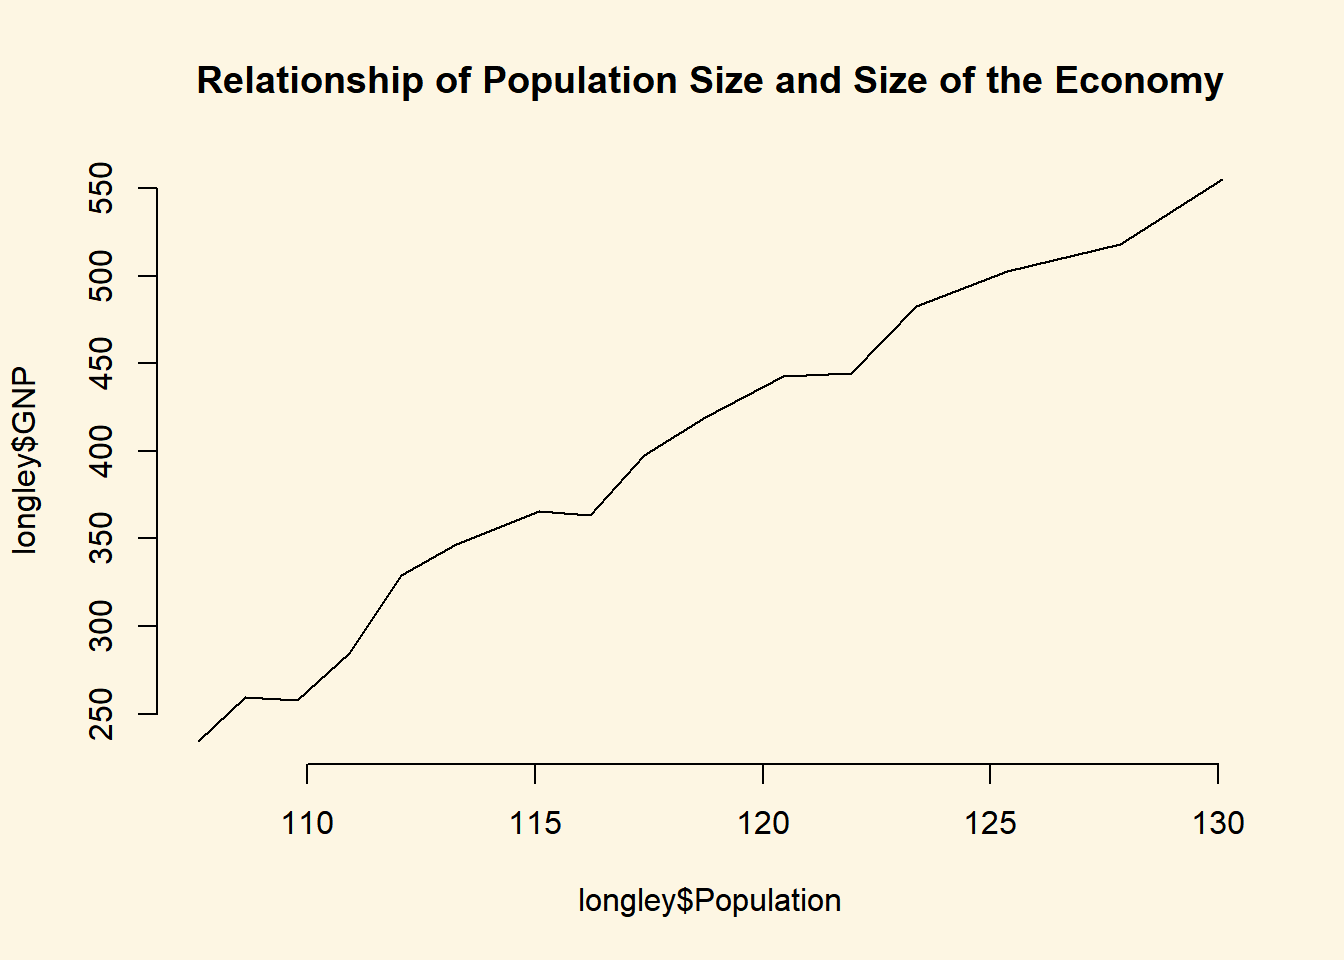
\includegraphics{statistics1_files/figure-latex/unnamed-chunk-94-1.pdf}

\subsubsection{Exercise 7}\label{exercise-7-1}

Use the help function to find out how to label the y-axis ``wealth'' and
the x-axis ``population''.

\begin{Shaded}
\begin{Highlighting}[]
\NormalTok{?plot}
\end{Highlighting}
\end{Shaded}

The \texttt{?} is short for the \texttt{help()} function. We see that
the \texttt{xlab} argument lets us label the x-axis and the
\texttt{ylab} argument lets us label the y-axis. We do so below.

\begin{Shaded}
\begin{Highlighting}[]
\KeywordTok{plot}\NormalTok{(}
  \DataTypeTok{y =}\NormalTok{ longley}\OperatorTok{$}\NormalTok{GNP, }\CommentTok{# y-axis variable}
  \DataTypeTok{x =}\NormalTok{ longley}\OperatorTok{$}\NormalTok{Population, }\CommentTok{# x-axis variable}
  \DataTypeTok{type =} \StringTok{"l"}\NormalTok{, }\CommentTok{# produce a line plot}
  \DataTypeTok{bty =} \StringTok{"n"}\NormalTok{, }\CommentTok{# no box around our plot}
  \DataTypeTok{main =} \StringTok{"Relationship of Population Size and Size of the Economy"}\NormalTok{,}
  \DataTypeTok{xlab =} \StringTok{"Population older than 14 years of age"}\NormalTok{,}
  \DataTypeTok{ylab =} \StringTok{"Gross national product"}
\NormalTok{)}
\end{Highlighting}
\end{Shaded}

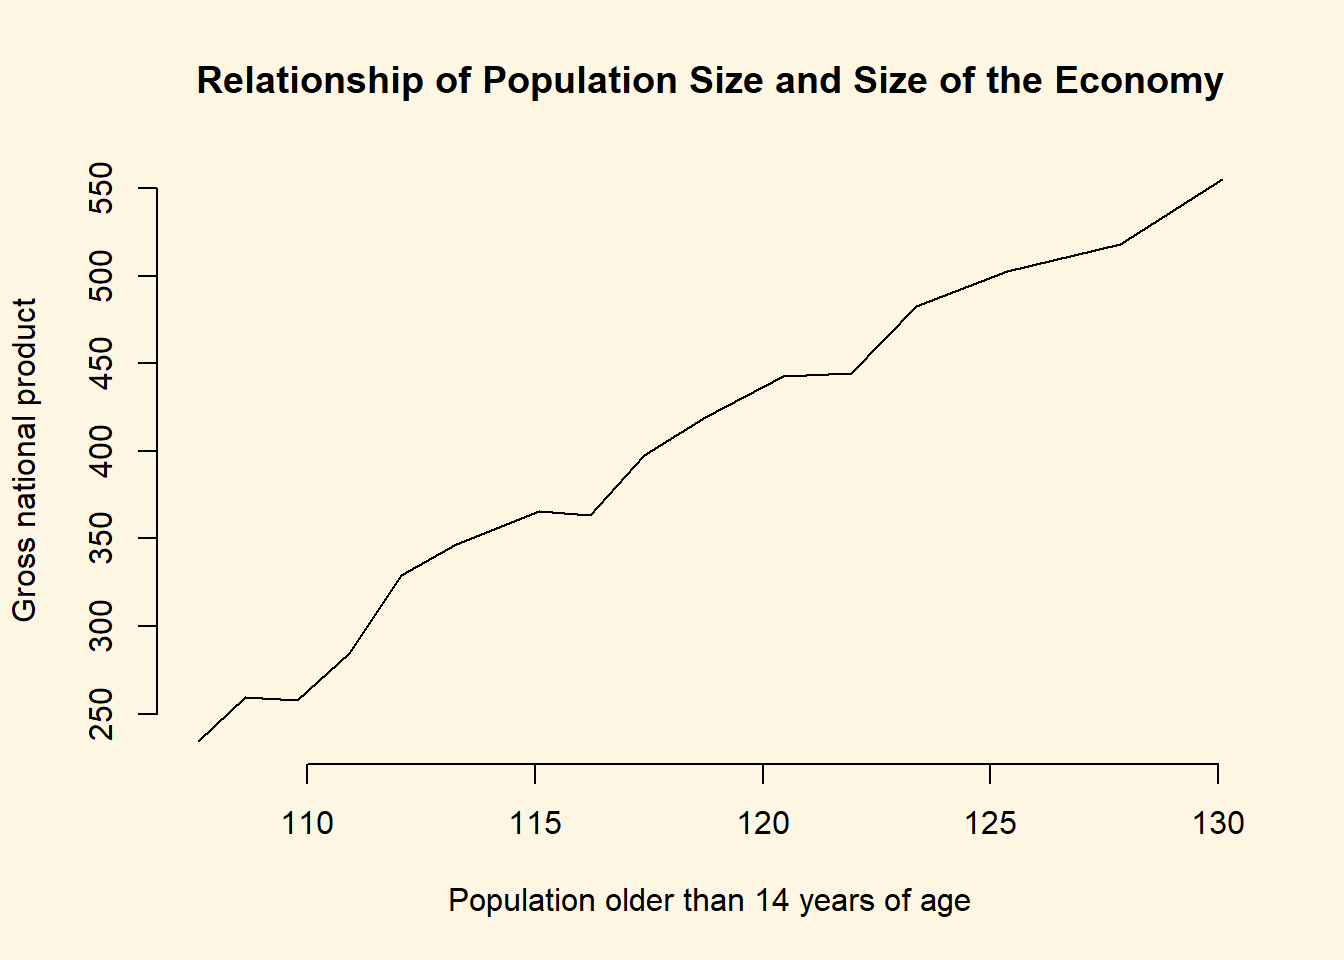
\includegraphics{statistics1_files/figure-latex/unnamed-chunk-96-1.pdf}

\subsubsection{Exercise 8}\label{exercise-8-1}

Create a boxplot showing the distribution of \emph{IMMBRIT} by each
party in the data and plot these in one plot next to each other.

To do that, we load the non-western foreigners dataset first.

Note: You have to set your working directory that R operates in to the
location of the dataset.

\begin{Shaded}
\begin{Highlighting}[]
\CommentTok{# load perception of non-western foreigners data}
\KeywordTok{load}\NormalTok{(}\StringTok{"BSAS_manip.RData"}\NormalTok{)}
\end{Highlighting}
\end{Shaded}

We have five parties in our dataset. We plot 5 boxplots next to each
other. Hence, we separate the plot window into 1 row and 5 columns.

\begin{Shaded}
\begin{Highlighting}[]
\CommentTok{# plot window to 1 row and 5 columns}
\KeywordTok{par}\NormalTok{(}\DataTypeTok{mfrow =} \KeywordTok{c}\NormalTok{(}\DecValTok{1}\NormalTok{, }\DecValTok{5}\NormalTok{))}
\KeywordTok{boxplot}\NormalTok{(data2}\OperatorTok{$}\NormalTok{IMMBRIT[ data2}\OperatorTok{$}\NormalTok{Cons }\OperatorTok{==}\StringTok{ }\DecValTok{1}\NormalTok{ ], }\DataTypeTok{frame.plot =} \OtherTok{FALSE}\NormalTok{, }\DataTypeTok{col =} \StringTok{"blue"}\NormalTok{, }\DataTypeTok{xlab =} \StringTok{"Tories"}\NormalTok{)}
\KeywordTok{boxplot}\NormalTok{(data2}\OperatorTok{$}\NormalTok{IMMBRIT[ data2}\OperatorTok{$}\NormalTok{Lab }\OperatorTok{==}\StringTok{ }\DecValTok{1}\NormalTok{ ], }\DataTypeTok{frame.plot =} \OtherTok{FALSE}\NormalTok{, }\DataTypeTok{col =} \StringTok{"red"}\NormalTok{, }\DataTypeTok{xlab =} \StringTok{"Labour"}\NormalTok{)}
\KeywordTok{boxplot}\NormalTok{(data2}\OperatorTok{$}\NormalTok{IMMBRIT[ data2}\OperatorTok{$}\NormalTok{SNP }\OperatorTok{==}\StringTok{ }\DecValTok{1}\NormalTok{ ], }\DataTypeTok{frame.plot =} \OtherTok{FALSE}\NormalTok{, }\DataTypeTok{col =} \StringTok{"yellow"}\NormalTok{, }\DataTypeTok{xlab =} \StringTok{"SNP"}\NormalTok{)}
\KeywordTok{boxplot}\NormalTok{(data2}\OperatorTok{$}\NormalTok{IMMBRIT[ data2}\OperatorTok{$}\NormalTok{Ukip }\OperatorTok{==}\StringTok{ }\DecValTok{1}\NormalTok{ ], }\DataTypeTok{frame.plot =} \OtherTok{FALSE}\NormalTok{, }\DataTypeTok{col =} \StringTok{"purple"}\NormalTok{, }\DataTypeTok{xlab =} \StringTok{"Ukip"}\NormalTok{)}
\KeywordTok{boxplot}\NormalTok{(data2}\OperatorTok{$}\NormalTok{IMMBRIT[ data2}\OperatorTok{$}\NormalTok{BNP }\OperatorTok{==}\StringTok{ }\DecValTok{1}\NormalTok{ ], }\DataTypeTok{frame.plot =} \OtherTok{FALSE}\NormalTok{, }\DataTypeTok{col =} \StringTok{"darkblue"}\NormalTok{, }\DataTypeTok{xlab =} \StringTok{"BNP"}\NormalTok{)}
\end{Highlighting}
\end{Shaded}

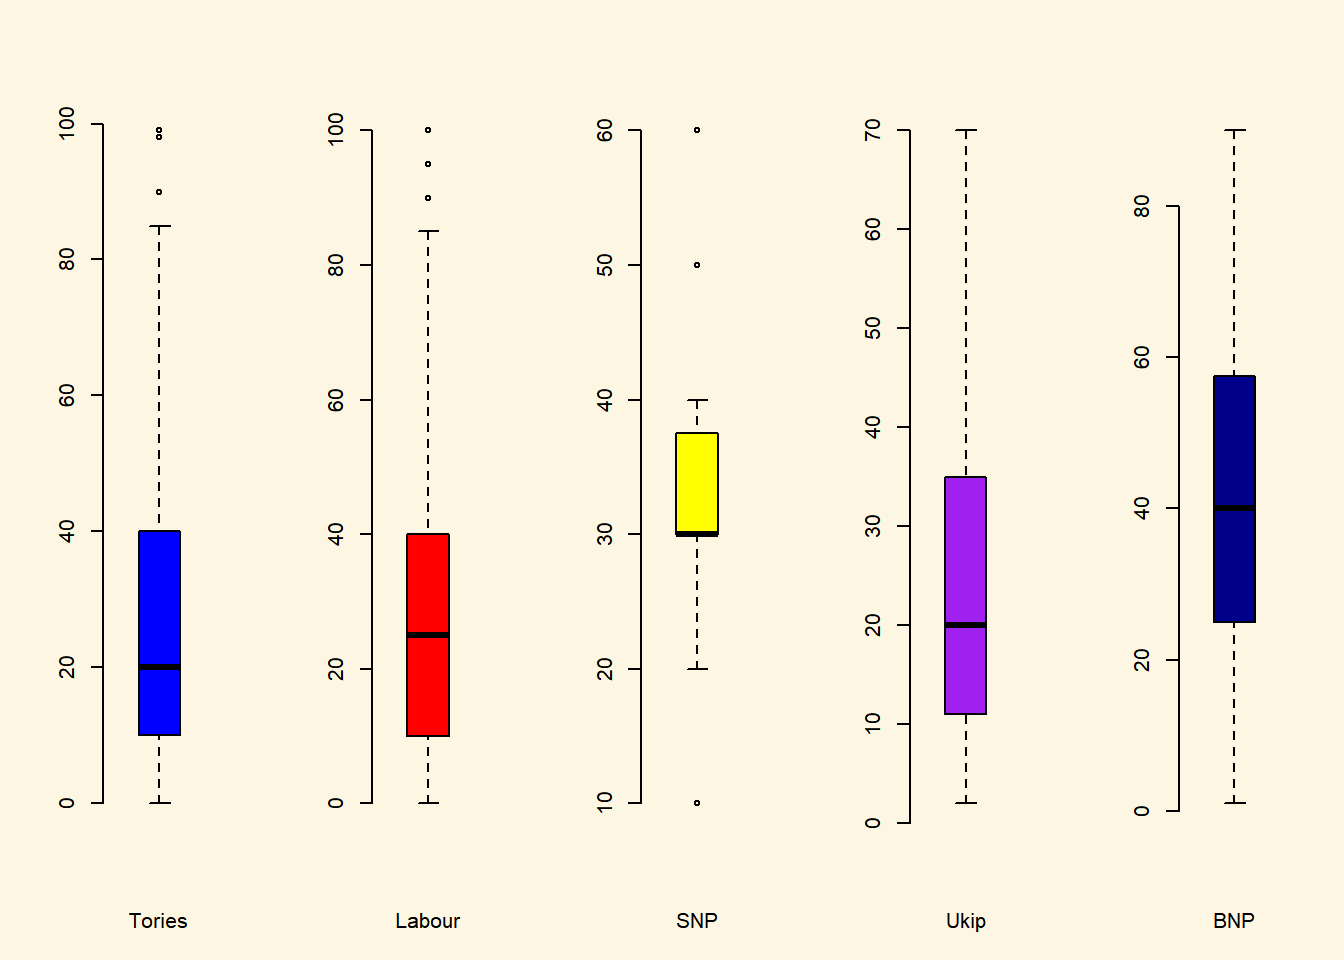
\includegraphics{statistics1_files/figure-latex/unnamed-chunk-98-1.pdf}

\subsubsection{Exercises 9 and 10}\label{exercises-9-and-10}

We combine the answer to questions 9 and 10.

Question from 9: Is there a difference between women and men in terms of
their subjective estimation of foreingers?

Question from 10: What is the difference between women and men?

Women's subjective estimate is the mean of \emph{IMMBRIT} across women
and equally, men's subjective estimate is the mean of \emph{IMMBRIT}
over all men. Let's get these numbers with the mean function and the
square brackets.

\begin{Shaded}
\begin{Highlighting}[]
\NormalTok{womens.mean <-}\StringTok{ }\KeywordTok{mean}\NormalTok{(data2}\OperatorTok{$}\NormalTok{IMMBRIT[ data2}\OperatorTok{$}\NormalTok{RSex }\OperatorTok{==}\StringTok{ }\DecValTok{2}\NormalTok{ ])}
\NormalTok{womens.mean}
\end{Highlighting}
\end{Shaded}

\begin{verbatim}
[1] 32.79159
\end{verbatim}

\begin{Shaded}
\begin{Highlighting}[]
\NormalTok{mens.mean <-}\StringTok{ }\KeywordTok{mean}\NormalTok{(data2}\OperatorTok{$}\NormalTok{IMMBRIT[ data2}\OperatorTok{$}\NormalTok{RSex }\OperatorTok{==}\StringTok{ }\DecValTok{1}\NormalTok{ ])}
\NormalTok{mens.mean}
\end{Highlighting}
\end{Shaded}

\begin{verbatim}
[1] 24.53766
\end{verbatim}

The difference between women and men is the difference in means. Let's
take the difference between them. The difference in means is often
referred to as the first difference.

\begin{Shaded}
\begin{Highlighting}[]
\NormalTok{first.difference <-}\StringTok{ }\NormalTok{womens.mean }\OperatorTok{-}\StringTok{ }\NormalTok{mens.mean}
\NormalTok{first.difference}
\end{Highlighting}
\end{Shaded}

\begin{verbatim}
[1] 8.253937
\end{verbatim}

Let's round that number. We don't like to see so many decimal places.
You should usually present precision up to the second decimal place. We
can use the \texttt{round()} function. The first argument is number to
round and the second is the amount of digits.

\begin{Shaded}
\begin{Highlighting}[]
\KeywordTok{round}\NormalTok{(first.difference, }\DecValTok{2}\NormalTok{)}
\end{Highlighting}
\end{Shaded}

\begin{verbatim}
[1] 8.25
\end{verbatim}

We do find a difference between men and women. On average, women's
estimate of the number of non-western foreingers is 8.25 greater than
men's estimate.

At this point we have established that there is a difference in our
sample. Samples are subject to sampling variability. That means, we
cannot yet say that the difference is systematic, i.e., British women,
generally, think that there are more non-western foreingers than British
men.

\subsubsection{Exercises 11}\label{exercises-11}

Could you form a hypothesis out of the relationship that you see if any
exists?

Our testable hypothesis could be: Women tend to overestimate the number
of foreigners more than men. In our sample, women tend to estimate on
the number of foreingers at

\section{Sampling and Distributions}\label{sampling-and-distributions}

\subsection{Seminar}\label{seminar-2}

In today's seminar, we work with missing data. We will turn a numerical
variable into a nominal data type. We then turn to distributions.

\begin{Shaded}
\begin{Highlighting}[]
\KeywordTok{rm}\NormalTok{(}\DataTypeTok{list=}\KeywordTok{ls}\NormalTok{())}
\KeywordTok{setwd}\NormalTok{(}\StringTok{"~/PUBLG100"}\NormalTok{)}
\end{Highlighting}
\end{Shaded}

\subsubsection{Loading Dataset in CSV
Format}\label{loading-dataset-in-csv-format}

In this seminar, we load a file in comma separated format
(\texttt{.csv}). The \texttt{load()} function from last week works only
for the native R file format. To load our csv-file, we use the
\href{https://stat.ethz.ch/R-manual/R-devel/library/utils/html/read.table.html}{\texttt{read.csv()}}
function.

Our data comes from the \href{http://qog.pol.gu.se/}{Quality of
Government Institute}. Let's have a look at the codebook:

Download the data
\href{https://github.com/philippbroniecki/statistics1/blob/master/data/QoG2012.csv?raw=TRUE}{here}

\begin{tabular}{l|l}
\hline
Variable & Description\\
\hline
h\_j & 1 if Free Judiciary\\
\hline
wdi\_gdpc & Per capita wealth in US dollars\\
\hline
undp\_hdi & Human development index (higher values = higher quality of life)\\
\hline
wbgi\_cce & Control of corruption index (higher values = more control of corruption)\\
\hline
wbgi\_pse & Political stability index (higher values = more stable)\\
\hline
former\_col & 1 = country was a colony once\\
\hline
lp\_lat\_abst & Latitude of country's captial divided by 90\\
\hline
\end{tabular}

\begin{Shaded}
\begin{Highlighting}[]
\NormalTok{world.data <-}\StringTok{ }\KeywordTok{read.csv}\NormalTok{(}\StringTok{"QoG2012.csv"}\NormalTok{)}
\end{Highlighting}
\end{Shaded}

Go ahead and (1) check the dimensions of \texttt{world.data}, (2) the
names of the variables of the dataset, (3) print the first six rows of
the dataset. (

\begin{Shaded}
\begin{Highlighting}[]
\CommentTok{# the dimensions: rows (observations) and columns (variables) }
\KeywordTok{dim}\NormalTok{(world.data)}
\end{Highlighting}
\end{Shaded}

\begin{verbatim}
[1] 194   7
\end{verbatim}

\begin{Shaded}
\begin{Highlighting}[]
\CommentTok{# the variable names}
\KeywordTok{names}\NormalTok{(world.data) }
\end{Highlighting}
\end{Shaded}

\begin{verbatim}
[1] "h_j"         "wdi_gdpc"    "undp_hdi"    "wbgi_cce"    "wbgi_pse"   
[6] "former_col"  "lp_lat_abst"
\end{verbatim}

\begin{Shaded}
\begin{Highlighting}[]
\CommentTok{# top 6 rows of the data}
\KeywordTok{head}\NormalTok{(world.data)}
\end{Highlighting}
\end{Shaded}

\begin{verbatim}
  h_j   wdi_gdpc undp_hdi   wbgi_cce   wbgi_pse former_col lp_lat_abst
1   0   628.4074       NA -1.5453584 -1.9343837          0   0.3666667
2   0  4954.1982    0.781 -0.8538115 -0.6026081          0   0.4555556
3   0  6349.7207    0.704 -0.7301510 -1.7336243          1   0.3111111
4  NA         NA       NA  1.3267342  1.1980436          0   0.4700000
5   0  2856.7517    0.381 -1.2065741 -1.4150945          1   0.1366667
6  NA 13981.9795    0.800  0.8624368  0.7084046          1   0.1892222
\end{verbatim}

\subsubsection{Missing Values}\label{missing-values}

Let's inspect the variable \emph{h\_j}. It is categorical, where 1
indicates that a country has a free judiciary. We use the
\texttt{table()} function to find the frequency in each category.

\begin{Shaded}
\begin{Highlighting}[]
\KeywordTok{table}\NormalTok{(world.data}\OperatorTok{$}\NormalTok{h_j)}
\end{Highlighting}
\end{Shaded}

\begin{verbatim}

  0   1 
105  64 
\end{verbatim}

We now know that 64 countries have a free judiciary and 105 countries do
not.

Conceptually the variable is nominal. To see how the variable is stored
in R, we can use the \texttt{str()} function.

\begin{Shaded}
\begin{Highlighting}[]
\KeywordTok{str}\NormalTok{(world.data}\OperatorTok{$}\NormalTok{h_j)}
\end{Highlighting}
\end{Shaded}

\begin{verbatim}
 int [1:194] 0 0 0 NA 0 NA 0 0 1 1 ...
\end{verbatim}

The function returns `int' which abbreviates `integer', i.e., a numeric
type. The function also shows us the first 10 realisations of the
variable. We se zeroes and ones which are the two categories. We also
see NA's which abbreviates not available. NAs are missing values. Values
can be missing for different reasons. For instance, a coder may have
forgotten to code whether a country had been colonised at some point in
its history or the country may be new and the categories, therefore,
don't apply. It is important for us that we cannot calculate with NAs.

There are different ways of dealing with NAs. We will always delete
missing values. Our dataset must maintain its rectangular structure.
Hence, when we delete a missing value from one variable, we delete it
for the entire row of the dataset. Consider the following example.

\begin{tabular}{l|l|l|l|l}
\hline
Row & Variable1 & Variable2 & Variable3 & Variable4\\
\hline
1 & 15 & 22 & 100 & 65\\
\hline
2 & NA & 17 & 26 & 75\\
\hline
3 & 27 & NA & 58 & 88\\
\hline
4 & NA & NA & 4 & NA\\
\hline
5 & 75 & 45 & 71 & 18\\
\hline
6 & 18 & 16 & 99 & 91\\
\hline
\end{tabular}

If we delete missing values from \emph{Variable1}, our dataset will look
like this:

\begin{tabular}{l|l|l|l|l}
\hline
Row & Variable1 & Variable2 & Variable3 & Variable4\\
\hline
1 & 15 & 22 & 100 & 65\\
\hline
3 & 27 & NA & 58 & 88\\
\hline
5 & 75 & 45 & 71 & 18\\
\hline
6 & 18 & 16 & 99 & 91\\
\hline
\end{tabular}

The new dataset is smaller than the original one. Rows 2 and 4 have been
deleted. When we drop missing values from one variable in our dataset,
we lose information on other variables as well. Therefore, you only want
to drop missing values on variables that you are interested in. Let's
drop the missing values on our variable \emph{h\_j}. We do this in
several steps.

First, we introduce the \texttt{is.na()} function. We supply a vector to
the function and it checks for every element, whether it is missing or
not. R returns true or false. Let's use the function on our variable.

\begin{Shaded}
\begin{Highlighting}[]
\KeywordTok{is.na}\NormalTok{(world.data}\OperatorTok{$}\NormalTok{h_j)}
\end{Highlighting}
\end{Shaded}

\begin{verbatim}
  [1] FALSE FALSE FALSE  TRUE FALSE  TRUE FALSE FALSE FALSE FALSE  TRUE
 [12] FALSE FALSE FALSE FALSE FALSE FALSE FALSE FALSE FALSE FALSE  TRUE
 [23]  TRUE FALSE FALSE FALSE FALSE FALSE FALSE FALSE FALSE FALSE FALSE
 [34] FALSE FALSE FALSE FALSE FALSE FALSE FALSE FALSE FALSE FALSE FALSE
 [45] FALSE FALSE FALSE FALSE FALSE FALSE FALSE FALSE FALSE FALSE FALSE
 [56] FALSE FALSE FALSE FALSE FALSE FALSE FALSE FALSE FALSE FALSE FALSE
 [67]  TRUE FALSE FALSE FALSE FALSE FALSE FALSE FALSE FALSE FALSE FALSE
 [78] FALSE FALSE FALSE FALSE FALSE FALSE FALSE FALSE FALSE FALSE FALSE
 [89] FALSE FALSE FALSE FALSE FALSE FALSE FALSE FALSE FALSE FALSE FALSE
[100]  TRUE FALSE FALSE FALSE FALSE FALSE FALSE FALSE  TRUE FALSE FALSE
[111] FALSE  TRUE FALSE FALSE FALSE FALSE FALSE FALSE FALSE  TRUE FALSE
[122] FALSE  TRUE FALSE FALSE FALSE FALSE FALSE  TRUE  TRUE  TRUE FALSE
[133] FALSE FALSE FALSE FALSE FALSE FALSE FALSE FALSE  TRUE FALSE FALSE
[144] FALSE FALSE  TRUE  TRUE  TRUE  TRUE  TRUE FALSE FALSE FALSE  TRUE
[155] FALSE FALSE FALSE FALSE FALSE FALSE FALSE FALSE FALSE FALSE  TRUE
[166] FALSE FALSE FALSE FALSE FALSE FALSE FALSE  TRUE FALSE FALSE FALSE
[177] FALSE FALSE  TRUE FALSE FALSE FALSE FALSE FALSE FALSE FALSE FALSE
[188] FALSE FALSE FALSE  TRUE FALSE FALSE FALSE
\end{verbatim}

To see the amount of missingness in the variable \emph{h\_j}, we can
combine \texttt{is.na()} with the \texttt{table()} function.

\begin{Shaded}
\begin{Highlighting}[]
\KeywordTok{table}\NormalTok{( }\KeywordTok{is.na}\NormalTok{(world.data}\OperatorTok{$}\NormalTok{h_j) )}
\end{Highlighting}
\end{Shaded}

\begin{verbatim}

FALSE  TRUE 
  169    25 
\end{verbatim}

So, we have 25 missing values on \emph{h\_j}. Our dataset has 194 rows.
Check your global environment to confirm this or use the \texttt{nrow()}
function. That means, if we drop all missing values from \emph{h\_j},
the our dataset \emph{world.data} will lose 25 rows.

Before we drop the missings, we introduce the \texttt{which()} function.
It returns the row indexes (the rows in the dataset) where some
condition is true. So if we use \texttt{which()} and \texttt{is.na()},
we get the row numbers in the \emph{world.data} dataset where values are
missing on \emph{h\_j}.

\begin{Shaded}
\begin{Highlighting}[]
\KeywordTok{which}\NormalTok{( }\KeywordTok{is.na}\NormalTok{( world.data}\OperatorTok{$}\NormalTok{h_j ) )}
\end{Highlighting}
\end{Shaded}

\begin{verbatim}
 [1]   4   6  11  22  23  67 100 108 112 120 123 129 130 131 141 146 147
[18] 148 149 150 154 165 173 179 191
\end{verbatim}

We said that our dataset will lose 25 rows. Let's use the
\texttt{length()} function to confirm that this is the case.

\begin{Shaded}
\begin{Highlighting}[]
\KeywordTok{length}\NormalTok{( }\KeywordTok{which}\NormalTok{( }\KeywordTok{is.na}\NormalTok{( world.data}\OperatorTok{$}\NormalTok{h_j ) ) ) }
\end{Highlighting}
\end{Shaded}

\begin{verbatim}
[1] 25
\end{verbatim}

We have, indeed, identified 25 rows that we want to delete from our
dataset.

The function \texttt{is.na()} returns ``TRUE'' if an observation is
missing. We can use the \texttt{!} operator so that the function returns
``TRUE'' if an observation is \textbf{not} missing. The \texttt{!} means
not.

Let's confirm this:

\begin{Shaded}
\begin{Highlighting}[]
\CommentTok{# true = observation is missing}
\KeywordTok{table}\NormalTok{( }\KeywordTok{is.na}\NormalTok{(world.data}\OperatorTok{$}\NormalTok{h_j) )}
\end{Highlighting}
\end{Shaded}

\begin{verbatim}

FALSE  TRUE 
  169    25 
\end{verbatim}

\begin{Shaded}
\begin{Highlighting}[]
\CommentTok{# true = observations is NOT missing}
\KeywordTok{table}\NormalTok{( }\OperatorTok{!}\KeywordTok{is.na}\NormalTok{(world.data}\OperatorTok{$}\NormalTok{h_j) )}
\end{Highlighting}
\end{Shaded}

\begin{verbatim}

FALSE  TRUE 
   25   169 
\end{verbatim}

We now drop the rows with missings on \emph{h\_j} by overwriting our
original dataset with a new dataset that is a copy of the old without
the missings. We use the square brackets to subset our dataset.

\begin{Shaded}
\begin{Highlighting}[]
\NormalTok{world.data <-}\StringTok{ }\NormalTok{world.data[ }\OperatorTok{!}\KeywordTok{is.na}\NormalTok{( world.data}\OperatorTok{$}\NormalTok{h_j ) , ] }
\end{Highlighting}
\end{Shaded}

Confirm that our new \emph{world.data} dataset has only 169 remaining.

``But what if we want our original dataset back,'' you ask. We have
overwritten the original. It is no longer in our work environment. We
have to reload the data set from the disk.

Let's do that:

\begin{Shaded}
\begin{Highlighting}[]
\NormalTok{world.data <-}\StringTok{ }\KeywordTok{read.csv}\NormalTok{(}\StringTok{"QoG2012.csv"}\NormalTok{)}
\end{Highlighting}
\end{Shaded}

Right, we now have all observations back. This is important. Let's say
we need to drop missings on a variable. We do is. If a later analysis
does not involve that variable, we want all the observations back.
Otherwise we would have thrown away valuable information. The smaller
our dataset, the less information it contains. Less information will
make it harder for us to detect systematic correlations. We have to
options. Either we reload the original dataset or we create a copy of
the original with a different name that we could use later on. Let's do
this.

\begin{Shaded}
\begin{Highlighting}[]
\NormalTok{full.dataset <-}\StringTok{ }\NormalTok{world.data}
\end{Highlighting}
\end{Shaded}

Let's drop missings on \emph{h\_j} in the \emph{world.data} dataset.

\begin{Shaded}
\begin{Highlighting}[]
\NormalTok{world.data <-}\StringTok{ }\NormalTok{world.data[ }\OperatorTok{!}\KeywordTok{is.na}\NormalTok{( world.data}\OperatorTok{$}\NormalTok{h_j ) , ] }
\end{Highlighting}
\end{Shaded}

Now, if we want the full dataset back, we can overwrite
\emph{world.data} with \emph{full.dataset}. The code would be the
following:

\begin{Shaded}
\begin{Highlighting}[]
\NormalTok{world.data <-}\StringTok{ }\NormalTok{full.dataset}
\end{Highlighting}
\end{Shaded}

If you ran this line. Delete missings from \emph{h\_j} in
\emph{world.data} again.

This data manipulation may seem boring but it is really important that
you know how to do this. Most of the work in data science is not running
statistical models but data manipulation. Most of the dataset you will
work with in your jobs, as a research assistant or on you dissertation
won't be cleaned for you. You will have to do that work. It takes time
and is sometimes frustrating. That's unfortunately the same for all of
us.

\subsubsection{Factor Variables}\label{factor-variables}

Categorical/nominal variables can be stored as numeric variables in R.
However, the values do not imply an ordering or relative importance. We
often store nominal variables as factor variables in R. A factor
variable is a nominal data type. The advantage of turning a variable
into a factor type is that we can assign labels to the categories and
that R will not calculate with the values assigned to the categories.

The function \texttt{factor()} lets us turn the variable into a nominal
data type. The first argument is the variable itself. The second are the
category labels and the third are the levels associated with the
categories. To know how those correspond, we have to scroll up and look
at the codebook.

We also overwrite the original numeric variable \texttt{h\_j} with our
nominal copy indicated by the assignment arrow \texttt{\textless{}-}.

\begin{Shaded}
\begin{Highlighting}[]
\CommentTok{# factorize judiciary variable}
\NormalTok{world.data}\OperatorTok{$}\NormalTok{h_j <-}\StringTok{ }\KeywordTok{factor}\NormalTok{(world.data}\OperatorTok{$}\NormalTok{h_j, }\DataTypeTok{labels =} \KeywordTok{c}\NormalTok{(}\StringTok{"controlled"}\NormalTok{, }\StringTok{"free"}\NormalTok{), }\DataTypeTok{levels =} \KeywordTok{c}\NormalTok{(}\DecValTok{0}\NormalTok{,}\DecValTok{1}\NormalTok{))}

\CommentTok{# frequency table of judiciary variable}
\KeywordTok{table}\NormalTok{(world.data}\OperatorTok{$}\NormalTok{h_j)}
\end{Highlighting}
\end{Shaded}

\begin{verbatim}

controlled       free 
       105         64 
\end{verbatim}

\subsubsection{Renaming Variables}\label{renaming-variables}

We want to rename \emph{h\_j} into something more meaningful. The new
name should be \emph{free.judiciary}. We can use the \texttt{names()}
function to get a vector of variable names.

\begin{Shaded}
\begin{Highlighting}[]
\KeywordTok{names}\NormalTok{(world.data)}
\end{Highlighting}
\end{Shaded}

\begin{verbatim}
[1] "h_j"         "wdi_gdpc"    "undp_hdi"    "wbgi_cce"    "wbgi_pse"   
[6] "former_col"  "lp_lat_abst"
\end{verbatim}

We want to change the first element of that vector. We know that we can
use square brackets to subset vectors. Let's display the first element
of the vector of variable names only.

\begin{Shaded}
\begin{Highlighting}[]
\KeywordTok{names}\NormalTok{(world.data)[}\DecValTok{1}\NormalTok{]}
\end{Highlighting}
\end{Shaded}

\begin{verbatim}
[1] "h_j"
\end{verbatim}

Now we simply change the name using the assignment arrow
\texttt{\textless{}-} and our new variable names goes in quotes.

\begin{Shaded}
\begin{Highlighting}[]
\KeywordTok{names}\NormalTok{(world.data)[}\DecValTok{1}\NormalTok{] <-}\StringTok{ "free.judiciary"}
\end{Highlighting}
\end{Shaded}

We now check the variable names to confirm that we successfully changed
the name.

\begin{Shaded}
\begin{Highlighting}[]
\KeywordTok{names}\NormalTok{(world.data)}
\end{Highlighting}
\end{Shaded}

\begin{verbatim}
[1] "free.judiciary" "wdi_gdpc"       "undp_hdi"       "wbgi_cce"      
[5] "wbgi_pse"       "former_col"     "lp_lat_abst"   
\end{verbatim}

\subsubsection{Distributions}\label{distributions}

A marginal distribution is the distribution of a variable by itself.
Let's look at the summary statistics of the United Nations Development
Index \emph{undp\_hdi} using the \texttt{summary()} function.

\begin{Shaded}
\begin{Highlighting}[]
\KeywordTok{summary}\NormalTok{(world.data}\OperatorTok{$}\NormalTok{undp_hdi)}
\end{Highlighting}
\end{Shaded}

\begin{verbatim}
   Min. 1st Qu.  Median    Mean 3rd Qu.    Max.    NA's 
 0.2730  0.5272  0.7455  0.6946  0.8350  0.9560       9 
\end{verbatim}

How nice. This returns summary stats. We see the range(minimum to
maximum). We see the interquartile range (1st quartile to 3rd quartile).
We also see mean and median. Finally, we see the number of NAs.

Oh we forgot. We said, when we drop missing on variable, we may lose
information when we work on a new variable. Let's restore our dataset
\emph{world.data} to its original state.

\begin{Shaded}
\begin{Highlighting}[]
\NormalTok{world.data <-}\StringTok{ }\NormalTok{full.dataset}
\end{Highlighting}
\end{Shaded}

Now, we check the summary stats again.

\begin{Shaded}
\begin{Highlighting}[]
\KeywordTok{summary}\NormalTok{(world.data}\OperatorTok{$}\NormalTok{undp_hdi)}
\end{Highlighting}
\end{Shaded}

\begin{verbatim}
   Min. 1st Qu.  Median    Mean 3rd Qu.    Max.    NA's 
 0.2730  0.5390  0.7510  0.6982  0.8335  0.9560      19 
\end{verbatim}

In the smaller dataset (where we had dropped missings from \emph{h\_j}),
we had 9 missings. Now, we have 19 missings. The difference is 10. Our
smaller dataset had 25 rows less than the bigger dataset. Therefore, we
would have thrown away 6 good observations. That is not nothing. It's 3
percent of our data.

Let's drop missing on \emph{undp\_hdi} and rename it to \emph{hdi}.

\begin{Shaded}
\begin{Highlighting}[]
\NormalTok{world.data <-}\StringTok{ }\NormalTok{world.data[ }\KeywordTok{which}\NormalTok{( }\OperatorTok{!}\KeywordTok{is.na}\NormalTok{(world.data}\OperatorTok{$}\NormalTok{undp_hdi) ) , ]}
\end{Highlighting}
\end{Shaded}

Let's change the name.

\begin{Shaded}
\begin{Highlighting}[]
\KeywordTok{names}\NormalTok{(world.data)[}\DecValTok{3}\NormalTok{] <-}\StringTok{ "hdi"}
\KeywordTok{names}\NormalTok{(world.data)}
\end{Highlighting}
\end{Shaded}

\begin{verbatim}
[1] "h_j"         "wdi_gdpc"    "hdi"         "wbgi_cce"    "wbgi_pse"   
[6] "former_col"  "lp_lat_abst"
\end{verbatim}

Let's take the mean of \emph{hdi}.

\begin{Shaded}
\begin{Highlighting}[]
\NormalTok{hdi.mean <-}\StringTok{ }\KeywordTok{mean}\NormalTok{( world.data}\OperatorTok{$}\NormalTok{hdi )}
\NormalTok{hdi.mean}
\end{Highlighting}
\end{Shaded}

\begin{verbatim}
[1] 0.69824
\end{verbatim}

The mean of \emph{hdi} is the mean in the sample. We would like the mean
of hdi in the population. Remember that sampling variability causes us
to estimate a different mean every time we take a new sample.

We learned that the means follow a distribution if we take the mean
repeatedly in different samples. In expectation the population mean is
the sample mean. How certain are we about the mean. Well, we need to
know how the sampling distribution looks like.

To find out we estimate the standard error of the mean. The standard
error is the standard deviation of the sampling distribution. The name
is not standard deviation but standard error to indicate that we are
talking about the distribution of a statistic (the mean) and not a
random variable.

The formula for the standard error of the mean is:

\[ s_{\bar{x}} = \frac{ \sigma }{ \sqrt(n) }  \]

The \(\sigma\) is the real population standard deviation of the random
variable \emph{hdi} which is unknown to us. We replace the population
standard deviation with our sample estimate of it.

\[ s_{\bar{x}} = \frac{ s }{ \sqrt(n) }  \]

The standard error of the mean estimate is then

\begin{Shaded}
\begin{Highlighting}[]
\NormalTok{se.hdi <-}\StringTok{ }\KeywordTok{sd}\NormalTok{(world.data}\OperatorTok{$}\NormalTok{hdi) }\OperatorTok{/}\StringTok{ }\KeywordTok{sqrt}\NormalTok{( }\KeywordTok{nrow}\NormalTok{(world.data) )}
\NormalTok{se.hdi}
\end{Highlighting}
\end{Shaded}

\begin{verbatim}
[1] 0.01362411
\end{verbatim}

Okay, so the mean is 0.69824 and the standard error of the mean is
0.0136241.

We know that the sampling distribution is approximately normal. That
means that 95 percent of all observations are within 1.96 standard
deviations (standard errors) of the mean.

\[ \bar{x} \pm 1.96 \times s_{\bar{x}} \]

So what is that in our case?

\begin{Shaded}
\begin{Highlighting}[]
\NormalTok{lower.bound <-}\StringTok{ }\NormalTok{hdi.mean }\OperatorTok{-}\StringTok{ }\FloatTok{1.96} \OperatorTok{*}\StringTok{ }\NormalTok{se.hdi}
\NormalTok{lower.bound}
\end{Highlighting}
\end{Shaded}

\begin{verbatim}
[1] 0.6715367
\end{verbatim}

\begin{Shaded}
\begin{Highlighting}[]
\NormalTok{upper.bound <-}\StringTok{ }\NormalTok{hdi.mean }\OperatorTok{+}\StringTok{ }\FloatTok{1.96} \OperatorTok{*}\StringTok{ }\NormalTok{se.hdi}
\NormalTok{upper.bound}
\end{Highlighting}
\end{Shaded}

\begin{verbatim}
[1] 0.7249432
\end{verbatim}

That now means the following. Were we to take samples of \emph{hdi}
again and again and again, then 95 percent of the time, the mean would
be in the range from 0.6715367 to 0.7249432.

What is a probability? ``The long-run relative frequency,'' you all
scream in unison. Given that definition, you can say: ``With 95 percent
probability, the mean is in the range 0.6715367 to 0.7249432.''

Sometimes people like to former way of phrasing this relationship better
than the latter. In this case you tell them: ``a probability is the
long-run relative frequency of an outcome.''

Now, let's visualise our sampling distribution. We haven't actually
taken many samples, so how could we visualise the sampling distribution?
Well, we know the sampling distribution looks normal. We know that the
mean is our mean estimate in the sample. And finally, we know that the
standard deviation is the standard error of the mean.

We can randomly draw values from a normal distribution with mean 0.69824
and standard deviation 0.0136241. We do this with the \texttt{rnorm()}
function. It's first argument is the number of values to draw at random
from the normal distribution. The second argument is the mean and the
third is the standard deviation.

Recall, that a normal distribution has two parameters that characterise
it completely: the mean and the standard deviation. So with those two we
can draw the distribution.

\begin{Shaded}
\begin{Highlighting}[]
\NormalTok{draw.of.hdi.means <-}\StringTok{ }\KeywordTok{rnorm}\NormalTok{( }\DecValTok{1000}\NormalTok{, }\DataTypeTok{mean =}\NormalTok{ hdi.mean, }\DataTypeTok{sd =}\NormalTok{ se.hdi )}
\end{Highlighting}
\end{Shaded}

We have just drawn 1000 mean values at random from the distribution that
looks like our sampling distribution.

\begin{Shaded}
\begin{Highlighting}[]
\KeywordTok{plot}\NormalTok{(}
 \KeywordTok{density}\NormalTok{( draw.of.hdi.means ),}
 \DataTypeTok{bty =} \StringTok{"n"}\NormalTok{,}
 \DataTypeTok{main =} \StringTok{"Sampling Distribution of HDI means"}
\NormalTok{)}
\end{Highlighting}
\end{Shaded}

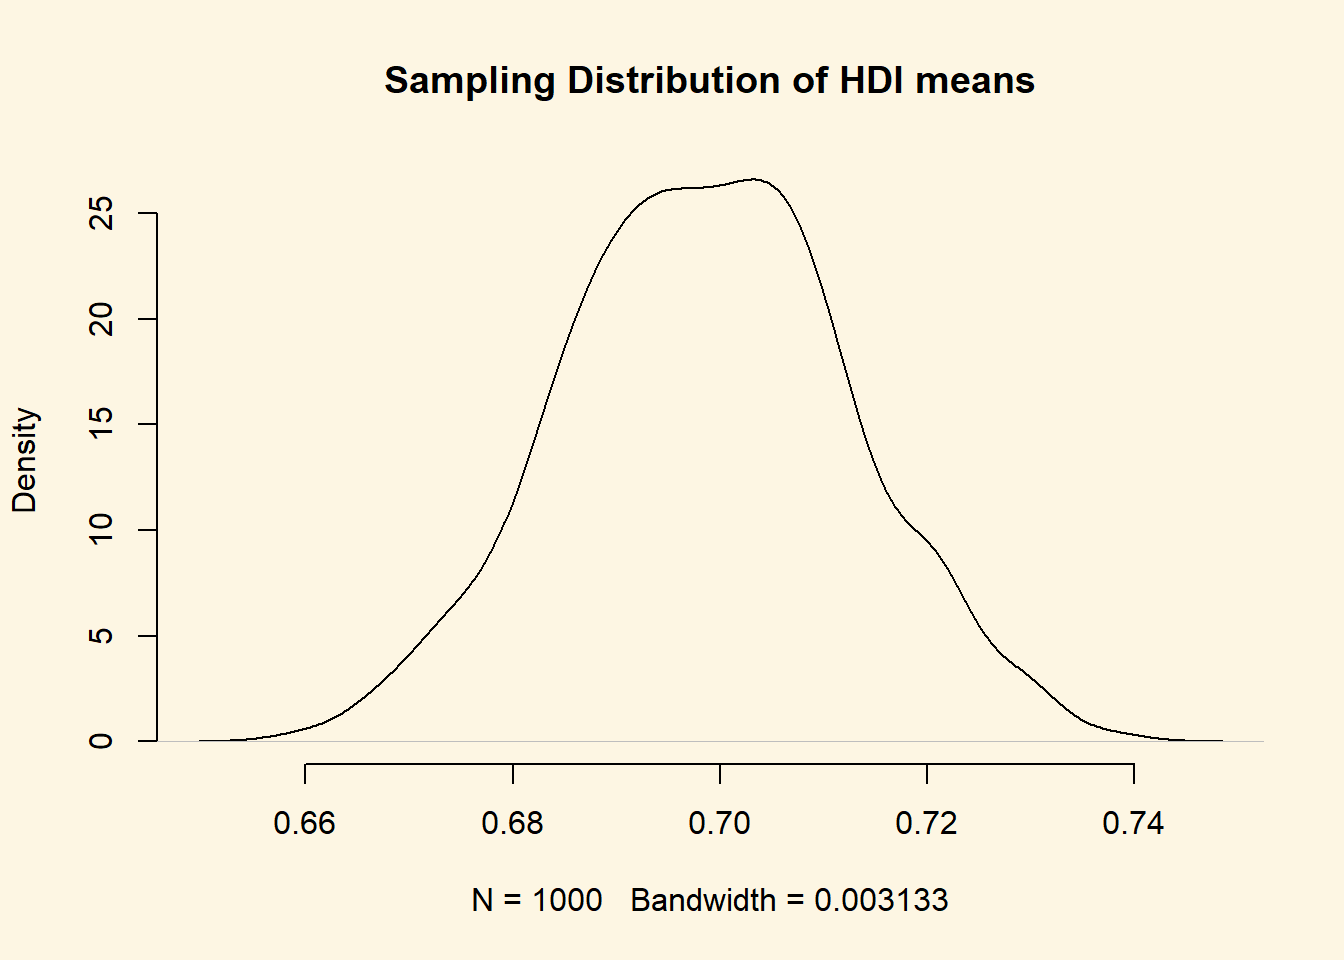
\includegraphics{statistics1_files/figure-latex/unnamed-chunk-136-1.pdf}

Beautiful Let's add the 95 percent confidence interval around our mean
estimate. The confidence interval quantifies our uncertainty. We said 95
percent of the time the mean would be in the interval from 0.6715367 to
0.7249432."

\begin{Shaded}
\begin{Highlighting}[]
\KeywordTok{abline}\NormalTok{( }\DataTypeTok{v =}\NormalTok{ lower.bound, }\DataTypeTok{lty =} \StringTok{"dashed"}\NormalTok{)}
\KeywordTok{abline}\NormalTok{( }\DataTypeTok{v =}\NormalTok{ upper.bound,  }\DataTypeTok{lty =} \StringTok{"dashed"}\NormalTok{)}
\end{Highlighting}
\end{Shaded}

You do not need to run the plot function again. You can just add to the
plot. Check the help function of \texttt{abline()} to see what its
arguments refer to.

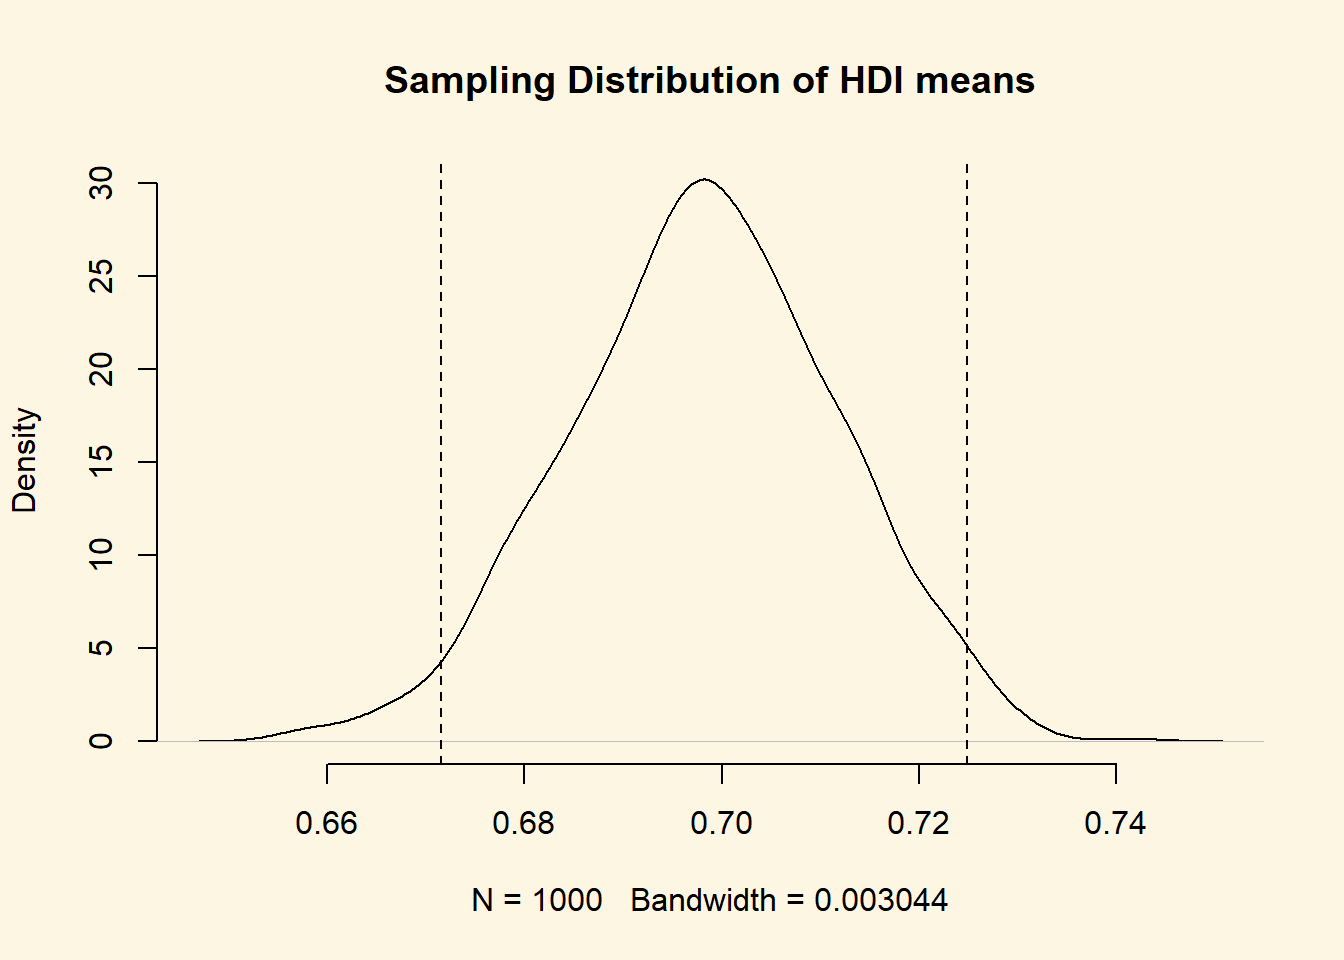
\includegraphics{statistics1_files/figure-latex/unnamed-chunk-138-1.pdf}

Fantastic! You can see that values below and above our confidence
interval are quite unlikely. Those values in the tails would not occur
often.

Not often, but not impossible.

Let's say that we wish know the probability that we take a sample and
our estimate of the mean is greater or equal 0.74. We would need to
integrate over the distribution from \(-\inf\) to 0.74. Fortunately R
has a function that does that for us. We need the \texttt{pnorm()}. It
calculates the probability of a value that is smaller or equal to the
value we specify. In other words, it gives us the probability from the
cumulative normal.

As the first argument \texttt{pnrom()} wants the value; 0.74 in our
case. The second and third arguments are the mean and the standard
deviation that characterise the normal distribution.

\begin{Shaded}
\begin{Highlighting}[]
\KeywordTok{pnorm}\NormalTok{(}\FloatTok{0.74}\NormalTok{, }\DataTypeTok{mean =}\NormalTok{ hdi.mean, }\DataTypeTok{sd =}\NormalTok{ se.hdi)}
\end{Highlighting}
\end{Shaded}

\begin{verbatim}
[1] 0.9989122
\end{verbatim}

What!? The probability to draw a mean 0.74 is 99.9 percent!? That cannot
be the value is so far in the tail of the distribution.

Well, this is the cumulative probability of drawing a value that is
equal to or smaller than 0.74. All probabilities sum to 1. So if we want
to know the probability of drawing a value that is greater than 0.74, we
subtract the probability, we just calculated, from 1.

\begin{Shaded}
\begin{Highlighting}[]
\DecValTok{1} \OperatorTok{-}\StringTok{ }\KeywordTok{pnorm}\NormalTok{(}\FloatTok{0.74}\NormalTok{, }\DataTypeTok{mean =}\NormalTok{ hdi.mean, }\DataTypeTok{sd =}\NormalTok{ se.hdi)}
\end{Highlighting}
\end{Shaded}

\begin{verbatim}
[1] 0.001087785
\end{verbatim}

Right, so the probability of getting a mean of \emph{hdi} in a sample is
0.1 percent.

\subsubsection{Conditional
Distributions}\label{conditional-distributions}

Let's look at \emph{hdi} by \emph{former\_col}. The variable
\emph{former\_col} is 1 if a country is a former colony and 0 otherwise.
The variable \emph{hdi} is continuous.

Before we start, we plot the marginal pdf of \emph{hdi}.

\begin{Shaded}
\begin{Highlighting}[]
\KeywordTok{plot}\NormalTok{(}
  \KeywordTok{density}\NormalTok{(world.data}\OperatorTok{$}\NormalTok{hdi),}
  \DataTypeTok{bty =} \StringTok{"n"}\NormalTok{,}
  \DataTypeTok{main =} \StringTok{"Marginal Distribution of HDI"}
\NormalTok{)}
\end{Highlighting}
\end{Shaded}

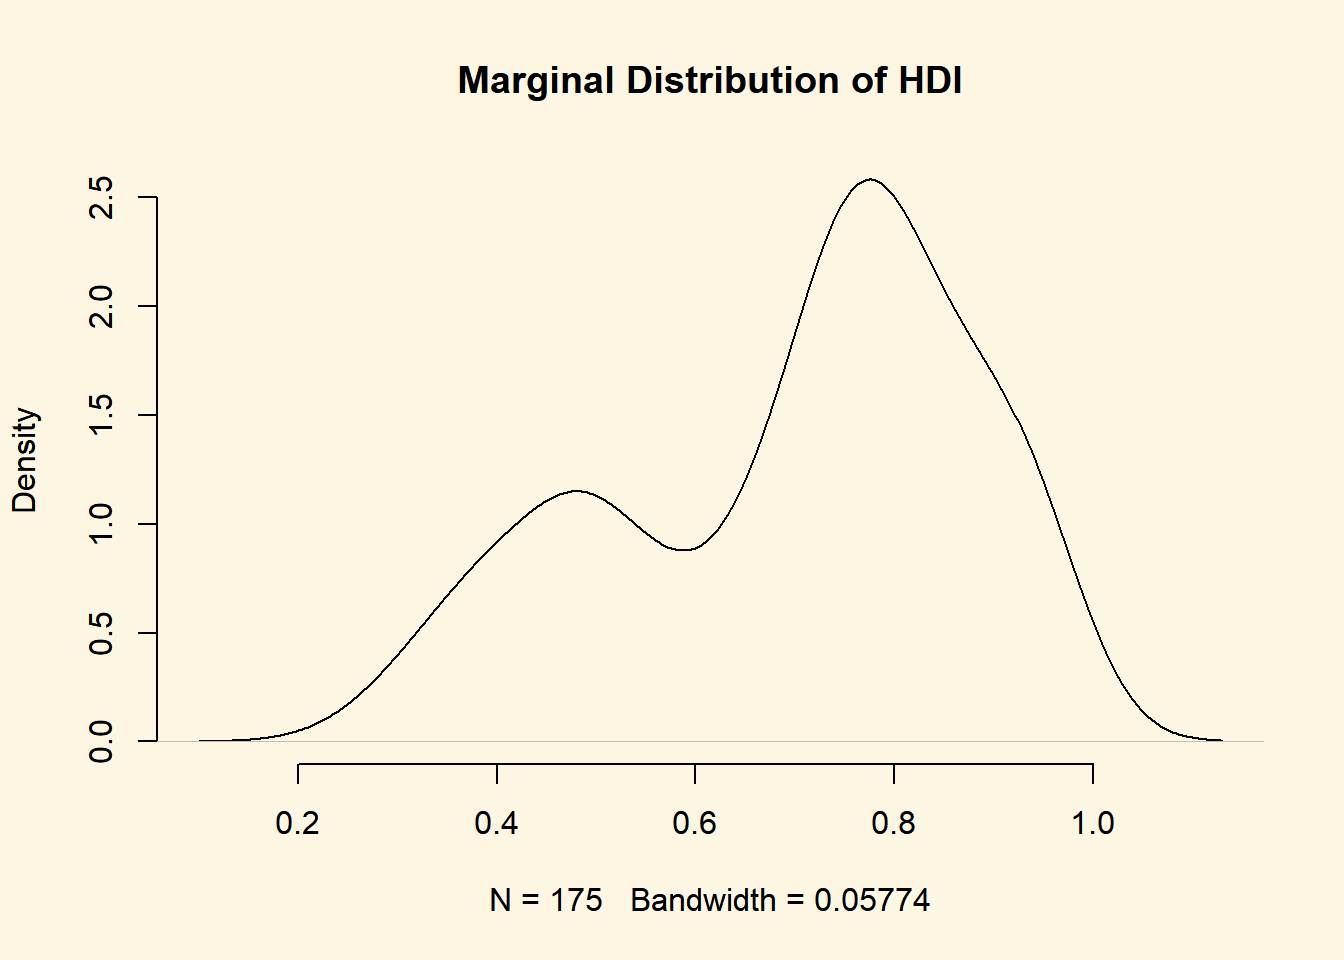
\includegraphics{statistics1_files/figure-latex/unnamed-chunk-141-1.pdf}

The distribution is bimodal. There is one peak at the higher development
end and one peak at the lower development end. Could it be that these
two peaks are conditional on whether a country was colonised or not?
Let's plot the conditional distributions.

\begin{Shaded}
\begin{Highlighting}[]
\KeywordTok{plot}\NormalTok{(}
  \KeywordTok{density}\NormalTok{(world.data}\OperatorTok{$}\NormalTok{hdi[world.data}\OperatorTok{$}\NormalTok{former_col }\OperatorTok{==}\StringTok{ }\DecValTok{0}\NormalTok{]),}
  \DataTypeTok{bty =} \StringTok{"n"}\NormalTok{,}
  \DataTypeTok{main =} \StringTok{"Conditional Distributions of HDI"}
\NormalTok{)}
\KeywordTok{lines}\NormalTok{(}\KeywordTok{density}\NormalTok{(world.data}\OperatorTok{$}\NormalTok{hdi[world.data}\OperatorTok{$}\NormalTok{former_col }\OperatorTok{==}\StringTok{ }\DecValTok{1}\NormalTok{]), }\DataTypeTok{lty =} \StringTok{"dashed"}\NormalTok{)}
\KeywordTok{legend}\NormalTok{(}\StringTok{"topleft"}\NormalTok{, }\KeywordTok{c}\NormalTok{(}\StringTok{"not colonised"}\NormalTok{, }\StringTok{"colonised"}\NormalTok{), }\DataTypeTok{lty =} \KeywordTok{c}\NormalTok{(}\StringTok{"solid"}\NormalTok{, }\StringTok{"dashed"}\NormalTok{))}
\end{Highlighting}
\end{Shaded}

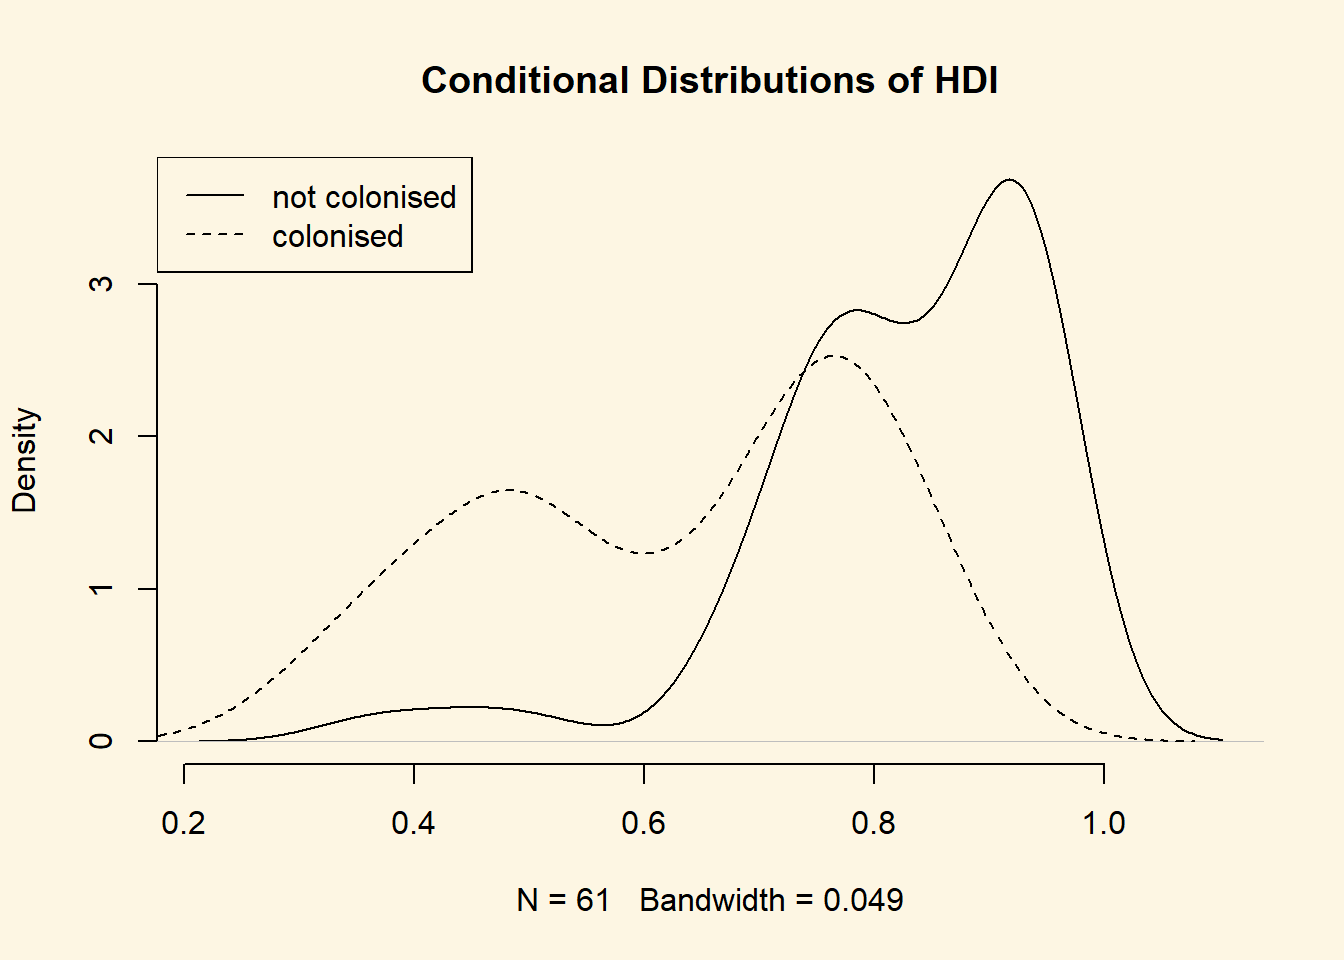
\includegraphics{statistics1_files/figure-latex/unnamed-chunk-142-1.pdf}

It's not quite like we expected. The distribution of human development
of not colonised countries is shifted to right of the distribution of
colonised countries and it is clearly narrower. Interestingly though,
the distribution of former colonies has a greater variance. Evidently,
some former colonies are doing very well and some are doing very poorly.
It seems like knowing whether a country was colonised or not tells us
something about its likely development but not enough. We cannot, e.g.,
say colonisation is the reason why countries do poorly. Probably, there
are differences among types of colonial institutions that were set up by
the colonisers.

Let's move on and examine the probability that a country has .8 or more
on \emph{hdi} given that it is a former colony.

We can get the cumulative probability with the \texttt{ecdf()} function.
It returns the empirical cumulative distribution, i.e., the cumulative
distribution of our data. We know that we can subset using square
brackets. That's all we need.

\begin{Shaded}
\begin{Highlighting}[]
\NormalTok{cumulative.p <-}\StringTok{ }\KeywordTok{ecdf}\NormalTok{(world.data}\OperatorTok{$}\NormalTok{hdi[ world.data}\OperatorTok{$}\NormalTok{former_col }\OperatorTok{==}\StringTok{ }\DecValTok{1}\NormalTok{ ])}
\DecValTok{1} \OperatorTok{-}\StringTok{ }\KeywordTok{cumulative.p}\NormalTok{(.}\DecValTok{8}\NormalTok{)}
\end{Highlighting}
\end{Shaded}

\begin{verbatim}
[1] 0.1666667
\end{verbatim}

Okay, the probability that a former colony has .8 or larger on the
\emph{hdi} is 16.6 percent. Go ahead figure out the probability for not
former colonies on your own.

\subsubsection{Exercises}\label{exercises-2}

\begin{enumerate}
\def\labelenumi{\arabic{enumi}.}
\tightlist
\item
  Create a script and call it assignment03. Save your script.
\item
  Load the \emph{world.data} dataset from your disk.
\item
  Rename the variable \emph{wdi\_gdpc} into \emph{gdpc}.
\item
  Delete missing values from \emph{gdpc}.
\item
  Inspect \emph{former\_col} and delete missing values from it.
\item
  Turn \emph{former\_col} into a factor variable with the appropriate
  lables.
\item
  Compute the probability that a county is richer than 55 000 per
  capita.
\item
  Compute the same probability given that a country is a former colony.
\item
  Compute the conditional expectation of wealth (gdp per capita) for a
  former colony.
\item
  Compute the conditional expectation of wealth for country that is not
  a former colony.
\item
  What is the probability that a former colony is 2 standard deviations
  below the mean wealth level?
\item
  What is the corresponding probability for a country that has not been
  colonised?
\item
  Compute the probability that a former colony is the wealth interval
  from 25 000 to 31 000.
\item
  Copmute the probability that a \textbf{not} former colony is in the
  top 2.5 percent of the wealth distribution.
\item
  At which wealth level is a country in the bottom 2.5 percent of the
  wealth distribution?
\end{enumerate}

\subsection{Solutions}\label{solutions-2}

\paragraph{Exercise 2}\label{exercise-2-1}

Load the world.data dataset from your disk.

\begin{Shaded}
\begin{Highlighting}[]
\NormalTok{world.data <-}\StringTok{ }\KeywordTok{read.csv}\NormalTok{(}\StringTok{"QoG2012.csv"}\NormalTok{)}
\end{Highlighting}
\end{Shaded}

\paragraph{Exercise 3}\label{exercise-3-2}

Rename the variable wdi\_gdpc into gdpc.

\begin{Shaded}
\begin{Highlighting}[]
\CommentTok{# to see all variable names}
\KeywordTok{names}\NormalTok{(world.data)}
\end{Highlighting}
\end{Shaded}

\begin{verbatim}
[1] "h_j"         "wdi_gdpc"    "undp_hdi"    "wbgi_cce"    "wbgi_pse"   
[6] "former_col"  "lp_lat_abst"
\end{verbatim}

\begin{Shaded}
\begin{Highlighting}[]
\CommentTok{# wdi_gdpc is the second variable. We rename the second element of the names vector}
\KeywordTok{names}\NormalTok{(world.data)[}\DecValTok{2}\NormalTok{] <-}\StringTok{ "gdpc"}
\end{Highlighting}
\end{Shaded}

\paragraph{Exercise 4}\label{exercise-4-2}

Delete missing values from gdpc.

\begin{Shaded}
\begin{Highlighting}[]
\CommentTok{# to check whether there are any missings or not}
\KeywordTok{summary}\NormalTok{(world.data}\OperatorTok{$}\NormalTok{gdpc)}
\end{Highlighting}
\end{Shaded}

\begin{verbatim}
   Min. 1st Qu.  Median    Mean 3rd Qu.    Max.    NA's 
  226.2  1768.0  5326.1 10184.1 12976.5 63686.7      16 
\end{verbatim}

\begin{Shaded}
\begin{Highlighting}[]
\CommentTok{# we have missings, let's make a copy of world.data before deleting}
\NormalTok{full.world.data <-}\StringTok{ }\NormalTok{world.data}
\CommentTok{# now let's delete the 16 rows with missings on gdpc}
\NormalTok{world.data <-}\StringTok{ }\NormalTok{world.data[ }\KeywordTok{which}\NormalTok{(}\OperatorTok{!}\KeywordTok{is.na}\NormalTok{(world.data}\OperatorTok{$}\NormalTok{gdpc)) , ]}
\end{Highlighting}
\end{Shaded}

\paragraph{Exercise 5}\label{exercise-5-2}

Inspect former\_col and delete missing values from it.

\begin{Shaded}
\begin{Highlighting}[]
\CommentTok{# we instpect the variable and check for missings}
\KeywordTok{summary}\NormalTok{(world.data}\OperatorTok{$}\NormalTok{former_col)}
\end{Highlighting}
\end{Shaded}

\begin{verbatim}
   Min. 1st Qu.  Median    Mean 3rd Qu.    Max. 
 0.0000  0.0000  1.0000  0.6348  1.0000  1.0000 
\end{verbatim}

\begin{Shaded}
\begin{Highlighting}[]
\CommentTok{# there are none, so there is nothing to delete}
\end{Highlighting}
\end{Shaded}

\paragraph{Exercise 6}\label{exercise-6-2}

Turn former\_col into a factor variable with the appropriate labels.

\begin{Shaded}
\begin{Highlighting}[]
\CommentTok{# we check the current storage type}
\KeywordTok{str}\NormalTok{(world.data}\OperatorTok{$}\NormalTok{former_col)}
\end{Highlighting}
\end{Shaded}

\begin{verbatim}
 int [1:178] 0 0 1 1 1 0 1 0 0 1 ...
\end{verbatim}

\begin{Shaded}
\begin{Highlighting}[]
\CommentTok{# it's numeric, so we change it to nominal}
\NormalTok{world.data}\OperatorTok{$}\NormalTok{former_col <-}\StringTok{ }\KeywordTok{factor}\NormalTok{(world.data}\OperatorTok{$}\NormalTok{former_col, }
                                \DataTypeTok{levels =} \KeywordTok{c}\NormalTok{(}\DecValTok{0}\NormalTok{,}\DecValTok{1}\NormalTok{), }
                                \DataTypeTok{labels =} \KeywordTok{c}\NormalTok{(}\StringTok{"not colonised"}\NormalTok{, }\StringTok{"former colony"}\NormalTok{ ))}
\CommentTok{# let's check the results}
\KeywordTok{table}\NormalTok{(world.data}\OperatorTok{$}\NormalTok{former_col)}
\end{Highlighting}
\end{Shaded}

\begin{verbatim}

not colonised former colony 
           65           113 
\end{verbatim}

Wait a minute. Is there something wrong here? The mean of the variable
is 0.63. That means 63 percent of all countries are former colonies.
Let's check whether we got that.

\begin{Shaded}
\begin{Highlighting}[]
\KeywordTok{table}\NormalTok{(world.data}\OperatorTok{$}\NormalTok{former_col) }\OperatorTok{/}\StringTok{ }\KeywordTok{sum}\NormalTok{(}\KeywordTok{table}\NormalTok{(world.data}\OperatorTok{$}\NormalTok{former_col))}
\end{Highlighting}
\end{Shaded}

\begin{verbatim}

not colonised former colony 
    0.3651685     0.6348315 
\end{verbatim}

Ah, that's correct. It's good to make sure, we did not mess up the
re-coding.

\paragraph{Exercise 8.}\label{exercise-8.}

Compute the probability that a county is richer than 55 000 per capita.

Wealth is never normally distributed. We don't even need to check. We
use the \texttt{ecdf()} function for the empirical cumulative
distribution.

The probability that a country is richer than 55 000 is 1 minus the
cumulative probability of 55000.

\begin{Shaded}
\begin{Highlighting}[]
\CommentTok{# get the empirical cumulative distribution of wealth}
\NormalTok{c.dist.of.wealth <-}\StringTok{ }\KeywordTok{ecdf}\NormalTok{(world.data}\OperatorTok{$}\NormalTok{gdpc)}
\CommentTok{# the prob}
\DecValTok{1} \OperatorTok{-}\StringTok{ }\KeywordTok{c.dist.of.wealth}\NormalTok{(}\DecValTok{55000}\NormalTok{)}
\end{Highlighting}
\end{Shaded}

\begin{verbatim}
[1] 0.01123596
\end{verbatim}

The probability is 0.01. Put differently 1 percent of countries is
richer than 55 000 US dollars per capita.

\paragraph{Exercise 8}\label{exercise-8-2}

Compute the same probability given that a country is a former colony.

The approach is similar but we want the conditional cumulative
distribution, where the condition is that a country is a former colony.

\begin{Shaded}
\begin{Highlighting}[]
\CommentTok{# conditional cumulative distribution}
\NormalTok{c.dist.of.wealth2 <-}\StringTok{ }\KeywordTok{ecdf}\NormalTok{(world.data}\OperatorTok{$}\NormalTok{gdpc[world.data}\OperatorTok{$}\NormalTok{former_col }\OperatorTok{==}\StringTok{ "former colony"}\NormalTok{])}
\DecValTok{1} \OperatorTok{-}\StringTok{ }\KeywordTok{c.dist.of.wealth2}\NormalTok{(}\DecValTok{55000}\NormalTok{)}
\end{Highlighting}
\end{Shaded}

\begin{verbatim}
[1] 0.008849558
\end{verbatim}

The probability is 0.009. The probability that a former colony is that
rich is slightly lower than that any country is.

\paragraph{Exercise 9}\label{exercise-9-1}

Compute the conditional expectation of wealth (gdp per capita) for a
former colony.

The conditional expectation is the mean of wealth among all former
colonies. We know how to do this from last week. We take the mean of
wealth and subset using square brackets.

\begin{Shaded}
\begin{Highlighting}[]
\KeywordTok{mean}\NormalTok{( world.data}\OperatorTok{$}\NormalTok{gdpc[world.data}\OperatorTok{$}\NormalTok{former_col }\OperatorTok{==}\StringTok{ "former colony"}\NormalTok{] )}
\end{Highlighting}
\end{Shaded}

\begin{verbatim}
[1] 6599.714
\end{verbatim}

The conditional expectation of wealth for former colonies is 6600 US
dollars per capita.

\paragraph{Exercise 10}\label{exercise-10-1}

Compute the conditional expectation of wealth for a country that is not
a former colony.

\begin{Shaded}
\begin{Highlighting}[]
\KeywordTok{mean}\NormalTok{( world.data}\OperatorTok{$}\NormalTok{gdpc[world.data}\OperatorTok{$}\NormalTok{former_col }\OperatorTok{==}\StringTok{ "not colonised"}\NormalTok{] )}
\end{Highlighting}
\end{Shaded}

\begin{verbatim}
[1] 16415.39
\end{verbatim}

The corresponding expectation for countries that have not been a colony
is 16415 US dollars.

\paragraph{Exercise 11}\label{exercise-11}

What is the probability that a former colony is 2 standard deviations
below the mean wealth level?

We first find out what a standard deviation of wealth is in the
conditional distribution of wealth for former colonies.

\begin{Shaded}
\begin{Highlighting}[]
\CommentTok{# standard deviation of wealth for former colonies}
\NormalTok{sd.wealth.cols <-}\StringTok{ }\KeywordTok{sd}\NormalTok{(world.data}\OperatorTok{$}\NormalTok{gdpc[world.data}\OperatorTok{$}\NormalTok{former_col }\OperatorTok{==}\StringTok{ "former colony"}\NormalTok{])}
\NormalTok{sd.wealth.cols}
\end{Highlighting}
\end{Shaded}

\begin{verbatim}
[1] 9783.914
\end{verbatim}

Interesting, the standard deviation is greater than the mean.
Apparently, former colonies are very different. Some do poorly and some
extremely well.

Doesn't this pose a problem for the task though? How can a country's
wealth be 2 standard deviations below the mean if the mean is smaller
than the standard deviation?

Well, that's not possible. Negative wealth does not exist. Consequently,
that probability is 0.

\paragraph{Exercise 12}\label{exercise-12}

We get the standard deviation of the wealth distribution of countries
that have not been colonised.

\begin{Shaded}
\begin{Highlighting}[]
\CommentTok{# standard deviation of wealth for not former colonies}
\NormalTok{sd.wealth.not.cols <-}\StringTok{ }\KeywordTok{sd}\NormalTok{(world.data}\OperatorTok{$}\NormalTok{gdpc[world.data}\OperatorTok{$}\NormalTok{former_col }\OperatorTok{==}\StringTok{ "not colonised"}\NormalTok{])}
\end{Highlighting}
\end{Shaded}

The result is similar to exercise 11. The mean is 16 415 and the
standard deviation is 13 766. 2 standard deviations below the mean would
be negative. The probability of that is 0.

\paragraph{Exercise 13}\label{exercise-13}

Compute the probability that a former colony is the wealth interval from
25 000 to 31 000.

We compute the cumulative probabilities that a country has 31 000 and 25
000 and then take the difference.

\begin{Shaded}
\begin{Highlighting}[]
\CommentTok{# cumulative probability of 31 000}
\NormalTok{p1 <-}\StringTok{ }\KeywordTok{c.dist.of.wealth2}\NormalTok{(}\DecValTok{31000}\NormalTok{)}
\CommentTok{# cumulative probability of 25 000}
\NormalTok{p2 <-}\StringTok{ }\KeywordTok{c.dist.of.wealth2}\NormalTok{(}\DecValTok{25000}\NormalTok{)}
\CommentTok{# probability of country in the interval}
\NormalTok{p1 }\OperatorTok{-}\StringTok{ }\NormalTok{p2}
\end{Highlighting}
\end{Shaded}

\begin{verbatim}
[1] 0
\end{verbatim}

The answer is again: 0. Let's have a look at the distribution to see
what's going on there.

\begin{Shaded}
\begin{Highlighting}[]
\KeywordTok{plot}\NormalTok{(}\KeywordTok{density}\NormalTok{( world.data}\OperatorTok{$}\NormalTok{gdpc[world.data}\OperatorTok{$}\NormalTok{former_col }\OperatorTok{==}\StringTok{ "former colony"}\NormalTok{] ))}
\end{Highlighting}
\end{Shaded}

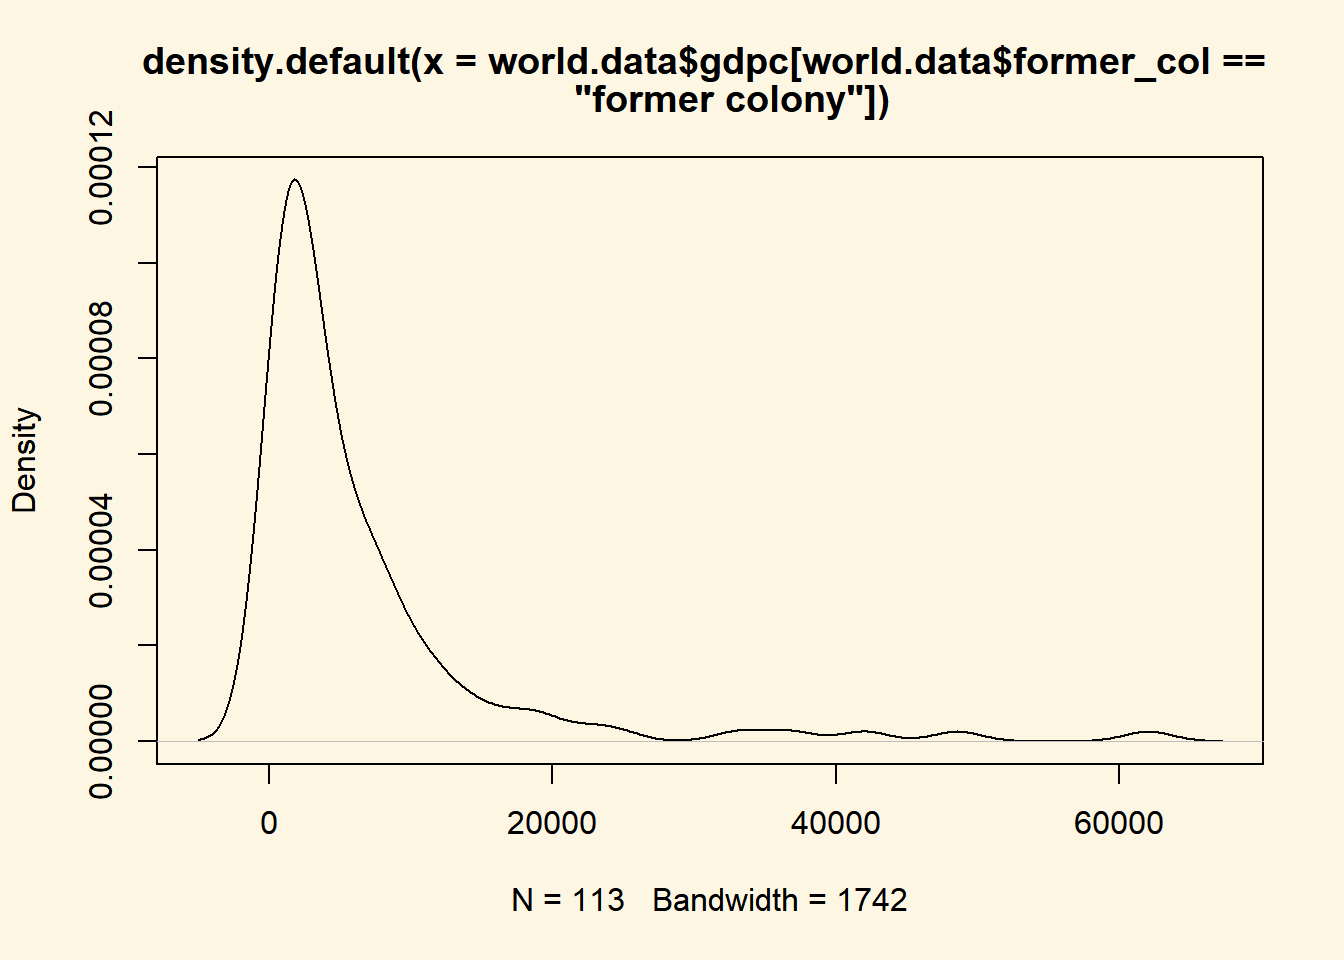
\includegraphics{statistics1_files/figure-latex/unnamed-chunk-159-1.pdf}

It seems like there are no countries in that interval. Let's check:

\begin{Shaded}
\begin{Highlighting}[]
\CommentTok{# let's look at summary stats first}
\KeywordTok{summary}\NormalTok{(world.data}\OperatorTok{$}\NormalTok{gdpc[ world.data}\OperatorTok{$}\NormalTok{former_col }\OperatorTok{==}\StringTok{ "former colony"}\NormalTok{  ])}
\end{Highlighting}
\end{Shaded}

\begin{verbatim}
   Min. 1st Qu.  Median    Mean 3rd Qu.    Max. 
  226.2  1263.7  3157.5  6599.7  7938.3 62005.6 
\end{verbatim}

\begin{Shaded}
\begin{Highlighting}[]
\CommentTok{# so there is at least 1 country that is richer. Let's look at all }
\CommentTok{# countries that are former colonies and also richer than 25 000}
\NormalTok{world.data[}\KeywordTok{which}\NormalTok{( world.data}\OperatorTok{$}\NormalTok{gdpc }\OperatorTok{>}\StringTok{ }\DecValTok{25000} \OperatorTok{&}\StringTok{ }\NormalTok{world.data}\OperatorTok{$}\NormalTok{former_col }\OperatorTok{==}\StringTok{ "former colony"}\NormalTok{), ]}
\end{Highlighting}
\end{Shaded}

\begin{verbatim}
    h_j     gdpc undp_hdi  wbgi_cce    wbgi_pse    former_col lp_lat_abst
24    0 48585.73    0.867 0.3304393  0.99980551 former colony   0.0477778
92    1 33079.87    0.838 1.0835209 -0.02684768 former colony   0.3255555
142   0 62005.56    0.833 0.9734111  0.76874268 former colony   0.2811111
156   1 36732.23    0.902 2.3715818  1.34370053 former colony   0.0135556
175   0 42004.04    0.824 1.0449655  0.80680293 former colony   0.2666667
\end{verbatim}

That's it. There are exactly zero countries in that interval.

Sub-setting with 2 conditions in square brackets may be new to you. We
did that with \texttt{\&} operator which means ``and''.

\paragraph{Exercise 14}\label{exercise-14}

Compute the probability that a not former colony is in the top 2.5
percent of the wealth distribution.

We find the value first. The top 2.5 percent are in the 97.5 percentile
of the distribution. We use the \texttt{quantile()} function to get the
value of the 97.5th percentile.

\begin{Shaded}
\begin{Highlighting}[]
\NormalTok{rich.countries <-}\StringTok{ }\KeywordTok{quantile}\NormalTok{(world.data}\OperatorTok{$}\NormalTok{gdpc[ world.data}\OperatorTok{$}\NormalTok{former_col }\OperatorTok{==}\StringTok{ "not colonised"}\NormalTok{], .}\DecValTok{975}\NormalTok{)}
\NormalTok{rich.countries}
\end{Highlighting}
\end{Shaded}

\begin{verbatim}
   97.5% 
41447.31 
\end{verbatim}

The value that puts a country in the top 2.5 percent of the conditional
wealth distribution (where the condition is that a country was not
colonised) is 41447 US dollars.

We now take the empirical cumulative distribution and get the
probability of being richer.

\begin{Shaded}
\begin{Highlighting}[]
\CommentTok{# conditional cumulative distribution}
\NormalTok{c.dist.of.wealth3 <-}\StringTok{ }\KeywordTok{ecdf}\NormalTok{(world.data}\OperatorTok{$}\NormalTok{gdpc[world.data}\OperatorTok{$}\NormalTok{former_col }\OperatorTok{==}\StringTok{ "not colonised"}\NormalTok{])}
\CommentTok{# conditional probability of being in the top 2.5 percent of not colonised countries}
\DecValTok{1} \OperatorTok{-}\StringTok{ }\KeywordTok{c.dist.of.wealth3}\NormalTok{(rich.countries)}
\end{Highlighting}
\end{Shaded}

\begin{verbatim}
[1] 0.03076923
\end{verbatim}

The probability is 0.03.

\paragraph{Exercise 15}\label{exercise-15}

At which wealth level is a country in the bottom 2.5 percent of the
wealth distribution?

The question asks for the wealth level that puts a country in the bottom
2.5 percent independent of whether it was a colony or not. The
\texttt{quantile()} function returns that value.

\begin{Shaded}
\begin{Highlighting}[]
\KeywordTok{quantile}\NormalTok{( world.data}\OperatorTok{$}\NormalTok{gdpc, .}\DecValTok{025}\NormalTok{ )}
\end{Highlighting}
\end{Shaded}

\begin{verbatim}
    2.5% 
526.8697 
\end{verbatim}

At 527 US dollars per capita, a country is in the bottom 2.5 percent of
the wealth distribution.

\section{T-test for Difference in Means and Hypothesis
Testing}\label{t-test-for-difference-in-means-and-hypothesis-testing}

\subsection{Seminar}\label{seminar-3}

Let's remove all objects from our workspace and set the working
directory.

\begin{Shaded}
\begin{Highlighting}[]
\KeywordTok{rm}\NormalTok{(}\DataTypeTok{list=}\KeywordTok{ls}\NormalTok{())}
\KeywordTok{setwd}\NormalTok{(}\StringTok{"~/statistics1"}\NormalTok{)}
\end{Highlighting}
\end{Shaded}

We load the data from the \href{http://qog.pol.gu.se/}{Quality of
Government Institute} again. Let's have a look at the codebook:

\begin{tabular}{l|l}
\hline
Variable & Description\\
\hline
h\_j & 1 if Free Judiciary\\
\hline
wdi\_gdpc & Per capita wealth in US dollars\\
\hline
undp\_hdi & Human development index (higher values = higher quality of life)\\
\hline
wbgi\_cce & Control of corruption index (higher values = more control of corruption)\\
\hline
wbgi\_pse & Political stability index (higher values = more stable)\\
\hline
former\_col & 1 = country was a colony once\\
\hline
lp\_lat\_abst & Latitude of country's captial divided by 90\\
\hline
\end{tabular}

Go ahead and load the data from last week yourself.

\begin{Shaded}
\begin{Highlighting}[]
\NormalTok{world.data <-}\StringTok{ }\KeywordTok{read.csv}\NormalTok{(}\StringTok{"QoG2012.csv"}\NormalTok{)}
\end{Highlighting}
\end{Shaded}

We can get summary statistics of each variable in the dataset by using
the \texttt{summary()} function over the dataset.

\begin{Shaded}
\begin{Highlighting}[]
\KeywordTok{summary}\NormalTok{(world.data)}
\end{Highlighting}
\end{Shaded}

\begin{verbatim}
      h_j            wdi_gdpc          undp_hdi         wbgi_cce       
 Min.   :0.0000   Min.   :  226.2   Min.   :0.2730   Min.   :-1.69953  
 1st Qu.:0.0000   1st Qu.: 1768.0   1st Qu.:0.5390   1st Qu.:-0.81965  
 Median :0.0000   Median : 5326.1   Median :0.7510   Median :-0.30476  
 Mean   :0.3787   Mean   :10184.1   Mean   :0.6982   Mean   :-0.05072  
 3rd Qu.:1.0000   3rd Qu.:12976.5   3rd Qu.:0.8335   3rd Qu.: 0.50649  
 Max.   :1.0000   Max.   :63686.7   Max.   :0.9560   Max.   : 2.44565  
 NA's   :25       NA's   :16        NA's   :19       NA's   :2         
    wbgi_pse          former_col      lp_lat_abst    
 Min.   :-2.46746   Min.   :0.0000   Min.   :0.0000  
 1st Qu.:-0.72900   1st Qu.:0.0000   1st Qu.:0.1343  
 Median : 0.02772   Median :1.0000   Median :0.2444  
 Mean   :-0.03957   Mean   :0.6289   Mean   :0.2829  
 3rd Qu.: 0.79847   3rd Qu.:1.0000   3rd Qu.:0.4444  
 Max.   : 1.67561   Max.   :1.0000   Max.   :0.7222  
                                     NA's   :7       
\end{verbatim}

\subsubsection{The Standard Error}\label{the-standard-error}

The standard error of an estimate quantifies uncertainty that is due to
sampling variability. Recall that we infer from a sample to the
population. Let's have a look at \emph{wdi\_gdpc} which is gdp per
capita. We re-name the variable to \emph{wealth}. Do so on your own.

\begin{Shaded}
\begin{Highlighting}[]
\KeywordTok{names}\NormalTok{(world.data)[}\DecValTok{2}\NormalTok{] <-}\StringTok{ "wealth"} 
\KeywordTok{names}\NormalTok{(world.data)}
\end{Highlighting}
\end{Shaded}

\begin{verbatim}
[1] "h_j"         "wealth"      "undp_hdi"    "wbgi_cce"    "wbgi_pse"   
[6] "former_col"  "lp_lat_abst"
\end{verbatim}

Now, have a look at the mean of the new \emph{wealth} variable.

\begin{Shaded}
\begin{Highlighting}[]
\KeywordTok{mean}\NormalTok{(world.data}\OperatorTok{$}\NormalTok{wealth)}
\end{Highlighting}
\end{Shaded}

\begin{verbatim}
[1] NA
\end{verbatim}

R returns NA because there are missing values on the \emph{wealth}
variable and we cannot calculate with NAs. For instance,
\texttt{2\ +\ NA} will return NA. We make a copy of the full data set
and then delete missing values. We did this last week. Go ahead do so on
your own.

\begin{Shaded}
\begin{Highlighting}[]
\CommentTok{# copy of the dataset}
\NormalTok{full.data <-}\StringTok{ }\NormalTok{world.data}

\CommentTok{# delete rows from dataset that have missings on wealth variable}
\NormalTok{world.data <-}\StringTok{ }\NormalTok{world.data[ }\OperatorTok{!}\KeywordTok{is.na}\NormalTok{(world.data}\OperatorTok{$}\NormalTok{wealth) , ]}
\end{Highlighting}
\end{Shaded}

Now, compute the mean of \emph{wealth} again.

\begin{Shaded}
\begin{Highlighting}[]
\KeywordTok{mean}\NormalTok{(world.data}\OperatorTok{$}\NormalTok{wealth)}
\end{Highlighting}
\end{Shaded}

\begin{verbatim}
[1] 10184.09
\end{verbatim}

The mean estimate in our sample is 10184.09. We are generally interested
in the population. Therefore, we infer from our sample to the
population. Our main problem is that samples are subject to sampling
variability. If we take another sample, our mean estimate would be
different. The standard error quantifies this type of uncertainty.

The formula for the standard error of the mean is:
\[ SE(\bar{Y}) = \frac{s_Y}{\sqrt{n}}  \]

Where \(s_Y\) is the standard deviation (of \emph{wealth}) and \(n\) is
the number of observations (of \emph{wealth}).

We compute the standard error in R:

\begin{Shaded}
\begin{Highlighting}[]
\NormalTok{se.y_bar <-}\StringTok{ }\NormalTok{(}\KeywordTok{sd}\NormalTok{(world.data}\OperatorTok{$}\NormalTok{wealth) }\OperatorTok{/}\StringTok{ }\KeywordTok{sqrt}\NormalTok{( }\KeywordTok{length}\NormalTok{(world.data}\OperatorTok{$}\NormalTok{wealth) ))}
\NormalTok{se.y_bar}
\end{Highlighting}
\end{Shaded}

\begin{verbatim}
[1] 922.7349
\end{verbatim}

The standard error is \textasciitilde{}922.73. The mean of the sampling
distribution is the population mean (or close to it --- the more samples
we take, the closer is the mean of the sampling distribution to the
population mean). The standard error is the average difference from the
population mean. We have taken 1 sample. When taking any random sample,
the average difference between the mean in that sample and the
population mean is the standard error.

We need the standard error for hypothesis testing. You will see how in
the following.

\subsubsection{T-test (one sample hypothesis
test)}\label{t-test-one-sample-hypothesis-test}

A knowledgeable friend declares that worldwide wealth stands at exactly
10 000 US dollars per capita today. We would like to know whether she is
right and tease her relentlessly if she isn't. To that end, we assume
that her claim is the population mean. We then estimate the mean of
\emph{wealth} in our sample. If the difference is large enough, so that
it is unlikely that it could have occurred by chance alone, we can
reject her claim.

So, first we take the mean of the \emph{wealth} variable.

\begin{Shaded}
\begin{Highlighting}[]
\KeywordTok{mean}\NormalTok{(world.data}\OperatorTok{$}\NormalTok{wealth)}
\end{Highlighting}
\end{Shaded}

\begin{verbatim}
[1] 10184.09
\end{verbatim}

Wow, our friend is quite close. Substantially, the difference of our
friends claim to our estimate is small but we could still find that the
difference is statistically significant (it's a noticeable systematic
difference).

Because we do not have information on all countries, our 10184.09 is an
estimate and the true population mean -- the population here would be
all countries in the world -- may be 10000 as our friend claims. We test
this statistically.

In statistics jargon: we would like to test whether our estimate is
statistically different from the 10000 figure (the null hypothesis)
suggested by our friend. Put differently, we would like to know the
probability that we estimate 10184.09 if the true mean of all countries
is 10000.

Recall, that the standard error of the mean (which is the estimate of
the true standard deviation of the population mean) is estimated as:

\[ \frac{s_{Y}}{\sqrt{n}} \]

Before we estimate the standard error, let's get \(n\) (the number of
observations). We have done this above but to make our code more
readable, we save the number of observations in an object that we call
\texttt{n}. Go ahead and do this on your own.

\begin{Shaded}
\begin{Highlighting}[]
\NormalTok{n <-}\StringTok{ }\KeywordTok{length}\NormalTok{(world.data}\OperatorTok{$}\NormalTok{wealth)}
\NormalTok{n}
\end{Highlighting}
\end{Shaded}

\begin{verbatim}
[1] 178
\end{verbatim}

With the function \texttt{length(world.data\$world)} we get all
observations in the data. Now, let's take the standard error of the mean
again.

\begin{Shaded}
\begin{Highlighting}[]
\NormalTok{se.y_bar <-}\StringTok{ }\KeywordTok{sd}\NormalTok{(world.data}\OperatorTok{$}\NormalTok{wealth) }\OperatorTok{/}\StringTok{ }\KeywordTok{sqrt}\NormalTok{(n)}
\end{Highlighting}
\end{Shaded}

We know that 1 standard error is one average deviation from the
population mean. The sampling distribution is approximately normal. 95
percent of the observations under the normal distribution are within 2
standard deviations of the mean.

We construct the confidence interval within which the population mean
lies with 95 percent probability in the following way. First, we take
our mean estimate of \emph{wealth}. That's the sample mean and not the
population mean. Second, we go 2 standard errors to the left of it. This
is the lower bound of our confidence interval. Third, we go 2 standard
deviations to the right of the sample mean. That is the upper bound of
our confidence interval.

The 95 percent confidence interval around the sample means gives the
interval within which the population mean lies with 95 percent
probability.

We want to know what the population mean is, right? Yes, that's right.
Therefore, we want the confidence interval to be as narrow as possible.
The narrower the confidence interval, the more precise we are about the
population mean. For instance, saying the population mean of income is
between 9 950 and 10 050 is more precise than saying the population mean
is between 5 000 and 15 000.

We construct the confidence interval with the standard error. That
means, the smaller the standard error, the more precise our estimate.
The formula for the 95 percent confidence interval is:

\[ \bar{Y} \pm 1.96 \times SE(\bar{Y}) \]

``Where does the 1.96 come from'', you ask. It's a critical value. More
on that later. For now, just recall that in a normal distribution 95
percent of all observations are within 1.96 standard errors of the mean.

We now construct our confidence interval. Our sample is large enough to
assume that the sampling distribution is approximately normal. So, we
can go \(1.96\) standard deviations to the left and to the right of the
mean to construct our \(95\%\) confidence interval.

\begin{Shaded}
\begin{Highlighting}[]
\CommentTok{# lower bound}
\NormalTok{lb <-}\StringTok{ }\KeywordTok{mean}\NormalTok{(world.data}\OperatorTok{$}\NormalTok{wealth) }\OperatorTok{-}\StringTok{ }\FloatTok{1.96} \OperatorTok{*}\StringTok{ }\NormalTok{se.y_bar}
\CommentTok{# upper bound}
\NormalTok{ub <-}\StringTok{ }\KeywordTok{mean}\NormalTok{(world.data}\OperatorTok{$}\NormalTok{wealth) }\OperatorTok{+}\StringTok{ }\FloatTok{1.96} \OperatorTok{*}\StringTok{ }\NormalTok{se.y_bar}
\CommentTok{# results (the population mean lies within this interval with 95% probability)}
\NormalTok{lb }\CommentTok{# lower bound}
\end{Highlighting}
\end{Shaded}

\begin{verbatim}
[1] 8375.531
\end{verbatim}

\begin{Shaded}
\begin{Highlighting}[]
\KeywordTok{mean}\NormalTok{(world.data}\OperatorTok{$}\NormalTok{wealth) }\CommentTok{# sample mean}
\end{Highlighting}
\end{Shaded}

\begin{verbatim}
[1] 10184.09
\end{verbatim}

\begin{Shaded}
\begin{Highlighting}[]
\NormalTok{ub }\CommentTok{# upper bound}
\end{Highlighting}
\end{Shaded}

\begin{verbatim}
[1] 11992.65
\end{verbatim}

You can make this look a little more like a table like so:

\begin{Shaded}
\begin{Highlighting}[]
\NormalTok{ci <-}\StringTok{ }\KeywordTok{cbind}\NormalTok{(}\DataTypeTok{lower_bound =}\NormalTok{ lb, }\DataTypeTok{mean =} \KeywordTok{mean}\NormalTok{(world.data}\OperatorTok{$}\NormalTok{wealth), }\DataTypeTok{upper_bound =}\NormalTok{ ub)}
\NormalTok{ci}
\end{Highlighting}
\end{Shaded}

\begin{verbatim}
     lower_bound     mean upper_bound
[1,]    8375.531 10184.09    11992.65
\end{verbatim}

The \texttt{cbind()} function stands for column-bind and creates a
\(1\times3\) matrix.

So we are \(95\%\) confident that the population average level of wealth
is between 8375.53 US dollars and 11992.65 US dollars. You can see that
we are not very certain about our estimate and we most definitely cannot
rule out that our friend is right (she claimed that the population mean
is 10 0000---that is within our interval). Hence, we cannot reject it.

A different way of describing our finding is to emphasize the logic of
(hypothetical) repeated sampling. In a process of repeated sampling we
can expect that the confidence interval that we calculate for each
sample will include the true population value \(95\%\) of the time. That
is equivalent to what we said earlier because a probability is the
long-run relative frequency of an outcome.

\paragraph{The t value}\label{the-t-value}

We now estimate the t value. Recall that our friend claimed that the
population mean was 10 000. This is the null hypothesis that we wish to
falsify. We estimated something else in our data, namely 10184.0910395.
The t value is the difference between our estimate (the result we get by
looking at data) and the population mean under the null hypothesis
divided by the standard error of the mean.

\[ \frac{ \bar{Y} - \mu_0 } {SE(\bar{Y})} \]

Where \(\bar{Y}\) is the mean in our data, \(\mu_0\) is the population
mean under the null hypothesis and \(SE(\bar{Y})\) is the standard error
of the mean.

Okay, let's compute this in R:

\begin{Shaded}
\begin{Highlighting}[]
\NormalTok{t.value <-}\StringTok{ }\NormalTok{(}\KeywordTok{mean}\NormalTok{(world.data}\OperatorTok{$}\NormalTok{wealth) }\OperatorTok{-}\StringTok{ }\DecValTok{10000}\NormalTok{) }\OperatorTok{/}\StringTok{ }\NormalTok{se.y_bar}
\NormalTok{t.value}
\end{Highlighting}
\end{Shaded}

\begin{verbatim}
[1] 0.1995059
\end{verbatim}

Look at the formula until you understand what is going on. In the
numerator we take the difference between our estimate and the population
mean under the null hypothesis. In expectation that difference should be
0---assuming that the null hypothesis is true. The larger that
difference, the less likely that the null hypothesis is true.

We divide by the standard error to transform the units of the difference
into standard deviations. Before we transformed the units, our
difference was in the units of whatever variable we are looking at (US
dollars in our example). By dividing by the standard error, we have
normed the variable. Its units are now standard deviations from the
mean.

Assume that the null hypothesis is true. In expectation the difference
between our estimate in the data and the population mean should be
\textbf{0 standard deviations}. The more standard deviations our
estimate is away from the population mean under the null hypothesis, the
less likely it is that the null hypothesis is true.

Within \textbf{1.96 standard deviations} from the mean lie 95 percent of
all observations. That means, it is very unlikely that the null
hypothesis is true, if the difference that we estimated is further than
1.96 standard deviations from the mean. ``How unlikely,'' you ask. We
would need the p value, for the exact probability. However, the
probability is less than 5 percent, if the estimated difference is more
than 1.96 standard deviations from the population mean under the null
hypothesis.

Back to our t value. We estimated a t value of 0.1995059. That means
that a sample estimate of 10184.0910395 is 0.1995059 standard deviations
from the population mean under the null hypothesis---which is 10 000 in
our sample.

Our t value suggests that our sample estimate would only be 0.1995059
standard deviations away from the population mean under the null. That
is not unlikely at all. We can only reject the null hypothesis if we are
more than 1.96 standard deviations away from the mean.

\paragraph{The p value}\label{the-p-value}

Let's estimate the precise p-value by calculating how likely it would be
to observe a t-statistic of 0.1995059 from a t-distribution with n - 1
(177) degrees of freedom.

The function \texttt{pt(t.value,\ df\ =\ n-1)} is the cumulative
probability that we get the t.value we put into the formula if the null
is true. The cumulative probability is estimated as the interval from
minus infinity to our t.value. So, 1 minus that probability is the
probability that we see anything larger (in the right tale of the
distribution). But we are testing whether the true mean is different
from 10000 (including smaller). Therefore, we want the probability that
we see a t.value in the right tale \emph{or} in the left tale of the
distribution. The distribution is symmetric. So we can just calculate
the probability of seeing a t-value in the right tale and multiply it by
2.

\begin{Shaded}
\begin{Highlighting}[]
\DecValTok{2}\OperatorTok{*}\StringTok{ }\NormalTok{( }\DecValTok{1} \OperatorTok{-}\StringTok{ }\KeywordTok{pt}\NormalTok{(t.value, }\DataTypeTok{df =}\NormalTok{ (n}\OperatorTok{-}\DecValTok{1}\NormalTok{) ))}
\end{Highlighting}
\end{Shaded}

\begin{verbatim}
[1] 0.8420961
\end{verbatim}

The p-value is way too large to reject the null hypothesis (the true
population mean is 10 000). If we specified an alpha-level of 0.05 in
advance, we would reject it only if the p-value was smaller than 0.05.
If we specified an alpha-level of 0.01 in advance, we would reject it
only if the p-value was smaller than 0.01, and so on.

Let's verify our result using the the t-test function \texttt{t.test()}.
The syntax of the function is:

\begin{verbatim}
t.test(formula, mu, alt, conf)
\end{verbatim}

Lets have a look at the arguments.

\begin{longtable}[]{@{}ll@{}}
\toprule
\begin{minipage}[b]{0.12\columnwidth}\raggedright\strut
Arguments\strut
\end{minipage} & \begin{minipage}[b]{0.78\columnwidth}\raggedright\strut
Description\strut
\end{minipage}\tabularnewline
\midrule
\endhead
\begin{minipage}[t]{0.12\columnwidth}\raggedright\strut
\texttt{formula}\strut
\end{minipage} & \begin{minipage}[t]{0.78\columnwidth}\raggedright\strut
Here, we input the vector that we calculate the mean of. For the
one-sample t test, in our example, this is the mean of \emph{wealth}.
For the t test for the difference in means, we would input both vectors
and separate them by a comma.\strut
\end{minipage}\tabularnewline
\begin{minipage}[t]{0.12\columnwidth}\raggedright\strut
\texttt{mu}\strut
\end{minipage} & \begin{minipage}[t]{0.78\columnwidth}\raggedright\strut
Here, we set the null hypothesis. The null hypothesis is that the true
population mean is 10000. Thus, we set \texttt{mu\ =\ 10000}.\strut
\end{minipage}\tabularnewline
\begin{minipage}[t]{0.12\columnwidth}\raggedright\strut
\texttt{alt}\strut
\end{minipage} & \begin{minipage}[t]{0.78\columnwidth}\raggedright\strut
There are two alternatives to the null hypothesis that the difference in
means is zero. The difference could either be smaller or it could be
larger than zero. To test against both alternatives, we set
\texttt{alt\ =\ "two.sided"}.\strut
\end{minipage}\tabularnewline
\begin{minipage}[t]{0.12\columnwidth}\raggedright\strut
\texttt{conf}\strut
\end{minipage} & \begin{minipage}[t]{0.78\columnwidth}\raggedright\strut
Here, we set the level of confidence that we want in rejecting the null
hypothesis. Common confidence intervals are: 95\%, 99\%, and
99.9\%---they correspond to alpha levels of 0.05, 0.01 and 0.001
respectively.\strut
\end{minipage}\tabularnewline
\bottomrule
\end{longtable}

\begin{Shaded}
\begin{Highlighting}[]
\KeywordTok{t.test}\NormalTok{(world.data}\OperatorTok{$}\NormalTok{wealth, }\DataTypeTok{mu =} \DecValTok{10000}\NormalTok{, }\DataTypeTok{alt =} \StringTok{"two.sided"}\NormalTok{) }
\end{Highlighting}
\end{Shaded}

\begin{verbatim}

    One Sample t-test

data:  world.data$wealth
t = 0.19951, df = 177, p-value = 0.8421
alternative hypothesis: true mean is not equal to 10000
95 percent confidence interval:
  8363.113 12005.069
sample estimates:
mean of x 
 10184.09 
\end{verbatim}

The results are similar. Therefore we can conclude that we are unable to
reject the null hypothesis suggested by our friend that the population
mean is equal to 10000. Let's see how we determine critical values.

\paragraph{Critical Values}\label{critical-values}

In social sciences, we usually operate with an alpha level of 0.05. That
means, we reject the null hypothesis if the p value is smaller than
0.05. Or put differently, we reject the null hypothesis if the 95
percent confidence interval does not include the population mean under
the null hypothesis---which is always the case if our estimate is
further than two standard errors from the mean under null hypothesis
(usually 0).

We said earlier that the critical value is 1.96 for an alpha level of
0.05. That is true in large samples where the distribution of the t
value follows a normal distribution. 95 percent of all observations are
within 1.96 standard deviations of the mean.

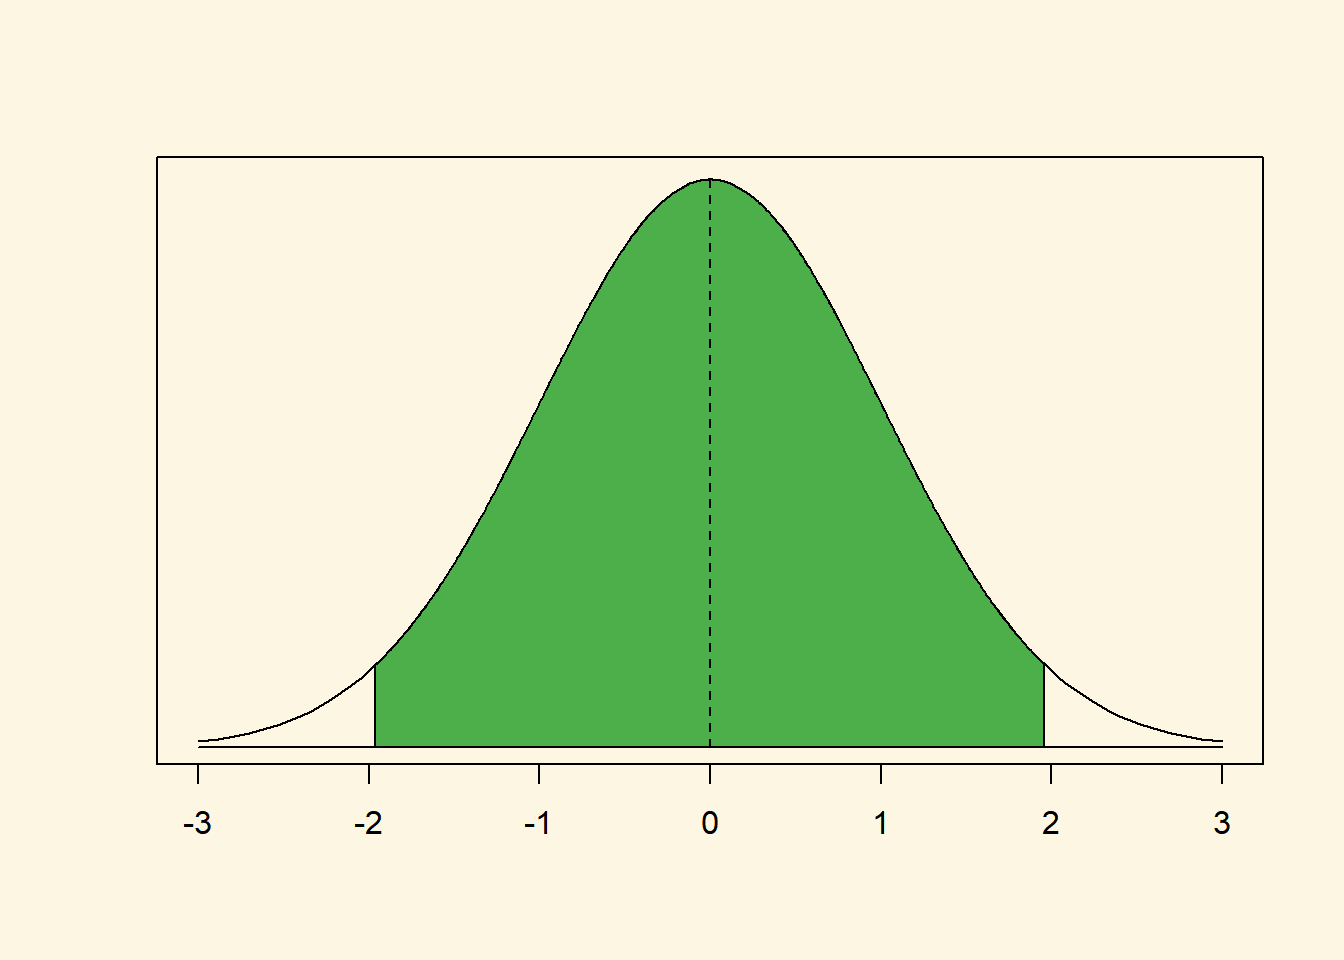
\includegraphics{statistics1_files/figure-latex/unnamed-chunk-184-1.pdf}

The green area under the curve covers 95 percent of all observations.
There are 2.5 percent in each tail. We reject the null hypothesis if our
estimate is in the tails of the distribution. It must be further than
1.96 standard deviations from the mean. But how did we know that 95
percent of the area under the curve is within 1.96 standard deviations
from the mean?

Let's separate the curve in you mind into 3 pieces. The left tail covers
2.5 percent of the area under the curve. The green middle bit covers 95
percent and the right tail again 2.5 percent. Now we do this as
cumulative probabilities. The left tail ends at 2.5 percent cumulative
probability. The green area ends at 97.5 percent cumulative probability
and the right tail ends at 100 percent.

The critical value is were the left tail ends or the right tail starts
(looking at the curve from left to right). Let's get the value where the
cumulative probability is 2.5 percent---where the left tail ends.

\begin{Shaded}
\begin{Highlighting}[]
\CommentTok{#}
\KeywordTok{qnorm}\NormalTok{(}\FloatTok{0.025}\NormalTok{, }\DataTypeTok{mean =} \DecValTok{0}\NormalTok{, }\DataTypeTok{sd =} \DecValTok{1}\NormalTok{)}
\end{Highlighting}
\end{Shaded}

\begin{verbatim}
[1] -1.959964
\end{verbatim}

If you look at the x-axis of our curve that is indeed where the left
tail ends. We add a red dot to our graph to highlight it.

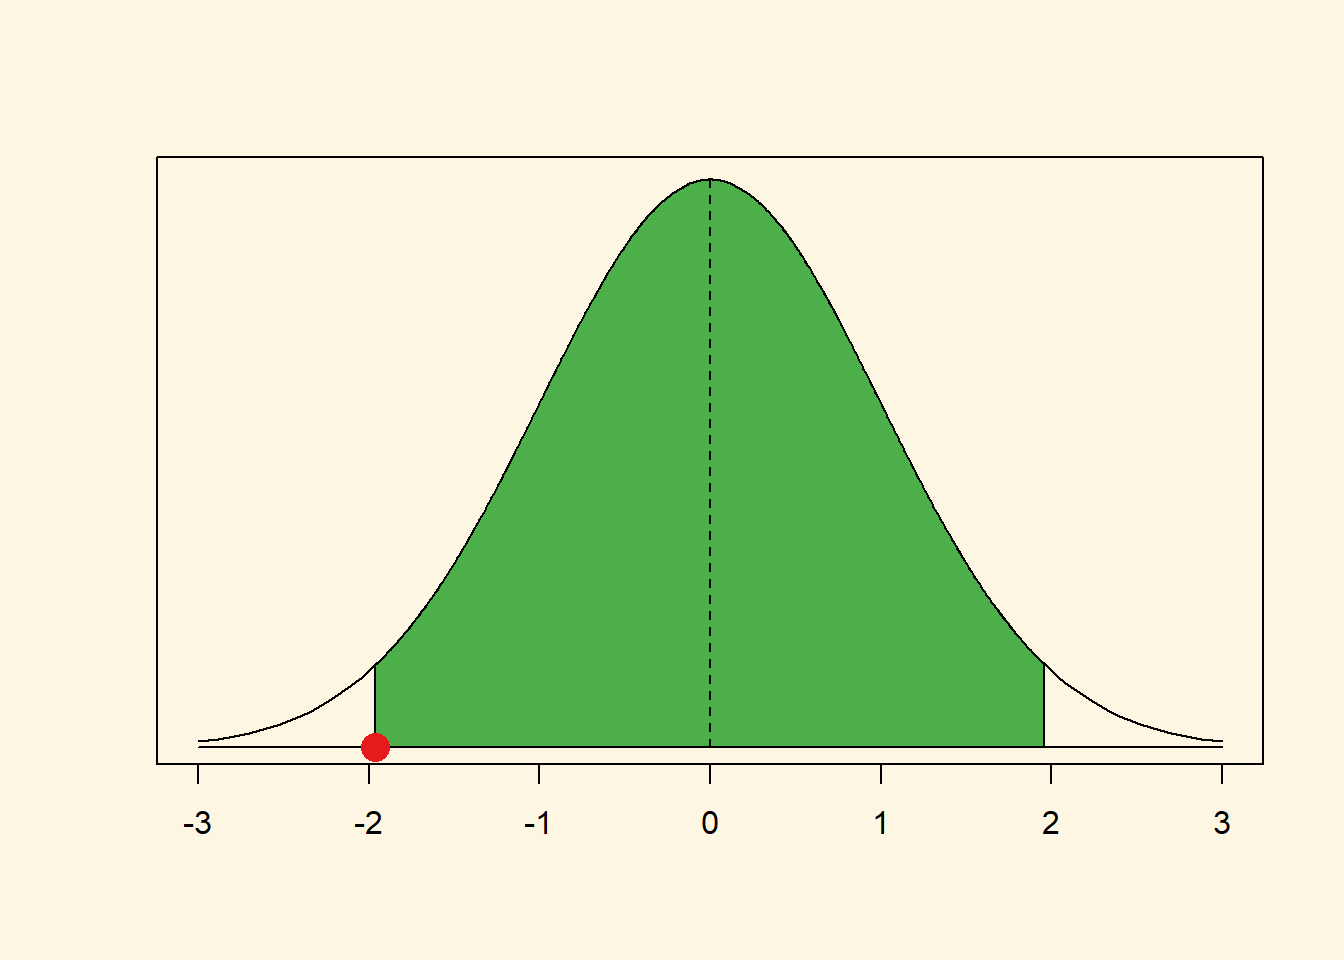
\includegraphics{statistics1_files/figure-latex/unnamed-chunk-186-1.pdf}

Now, let's get the critical value of where the right tail starts. That
is at the cumulative probability of 97.5 percent.

\begin{Shaded}
\begin{Highlighting}[]
\KeywordTok{qnorm}\NormalTok{(}\FloatTok{0.975}\NormalTok{, }\DataTypeTok{mean =} \DecValTok{0}\NormalTok{, }\DataTypeTok{sd =} \DecValTok{1}\NormalTok{)}
\end{Highlighting}
\end{Shaded}

\begin{verbatim}
[1] 1.959964
\end{verbatim}

As you can see, this is the same number, only positive instead of
negative. That's always the case because the normal distribution is
symmetric. Let's add that point in blue to our graph.

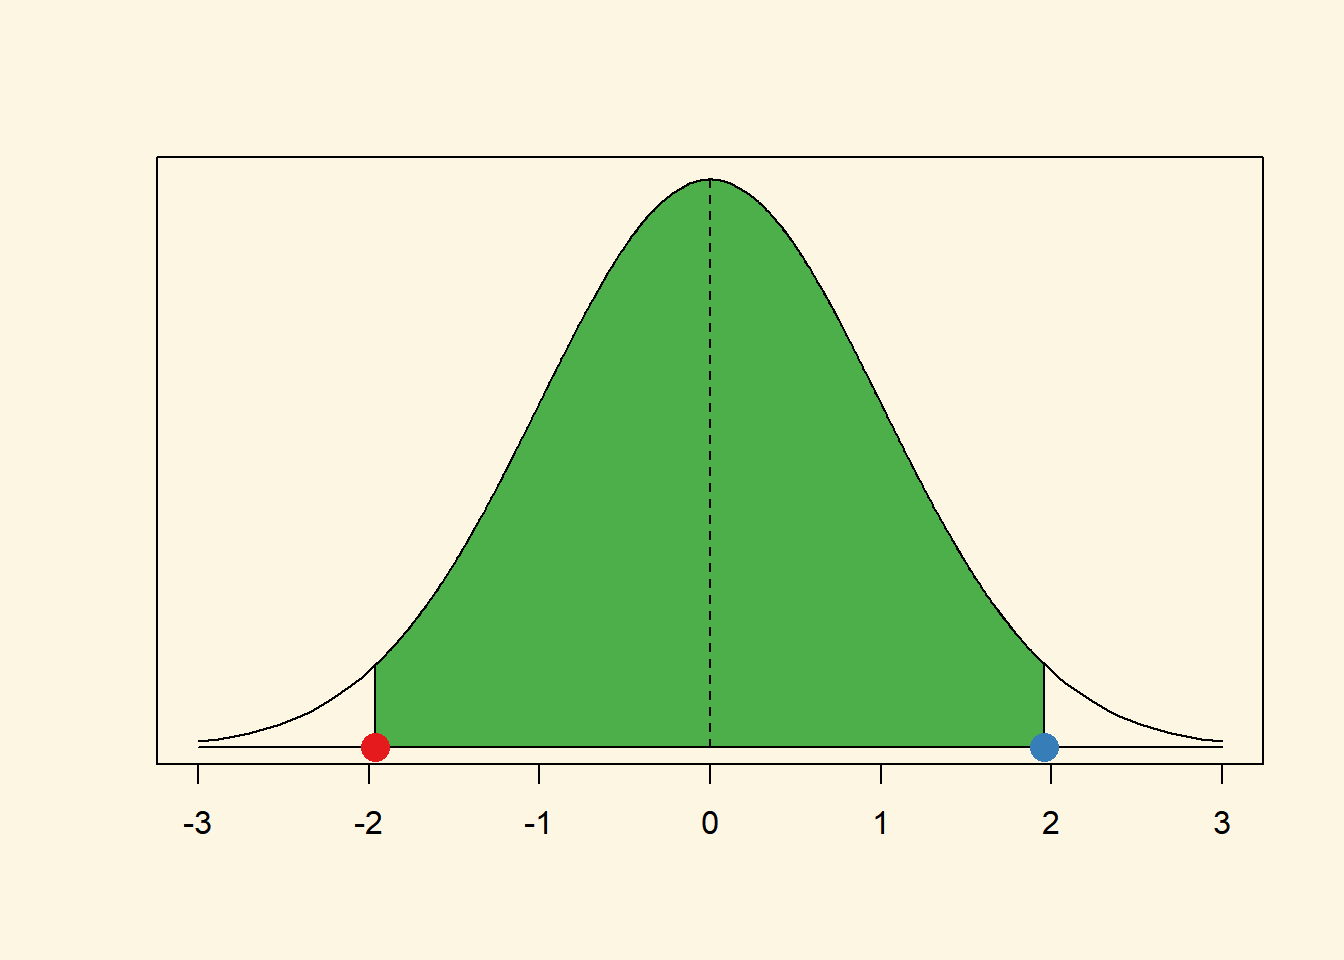
\includegraphics{statistics1_files/figure-latex/unnamed-chunk-188-1.pdf}

This is how we get the critical value for the 95 percent confidence
interval. By the way, back in the day you would have to look up critical
values in critical values tables at the end of statistics textbooks (you
can find the tables in Stock and Watson and Kellstedt and Whitten.)

As you can see our red and blue dots are the borders of the green area,
the 95 percent interval around the mean. You can get the critical values
for any other interval (e.g., the 99 percent interval) similar to what
we did just now.

We now do the same for the t distribution. In the t distribution, the
critical value depends on the shape of the t distribution which is
characterised by its degrees of freedom. Let's draw a t distribution
with 5 degrees of freedom.

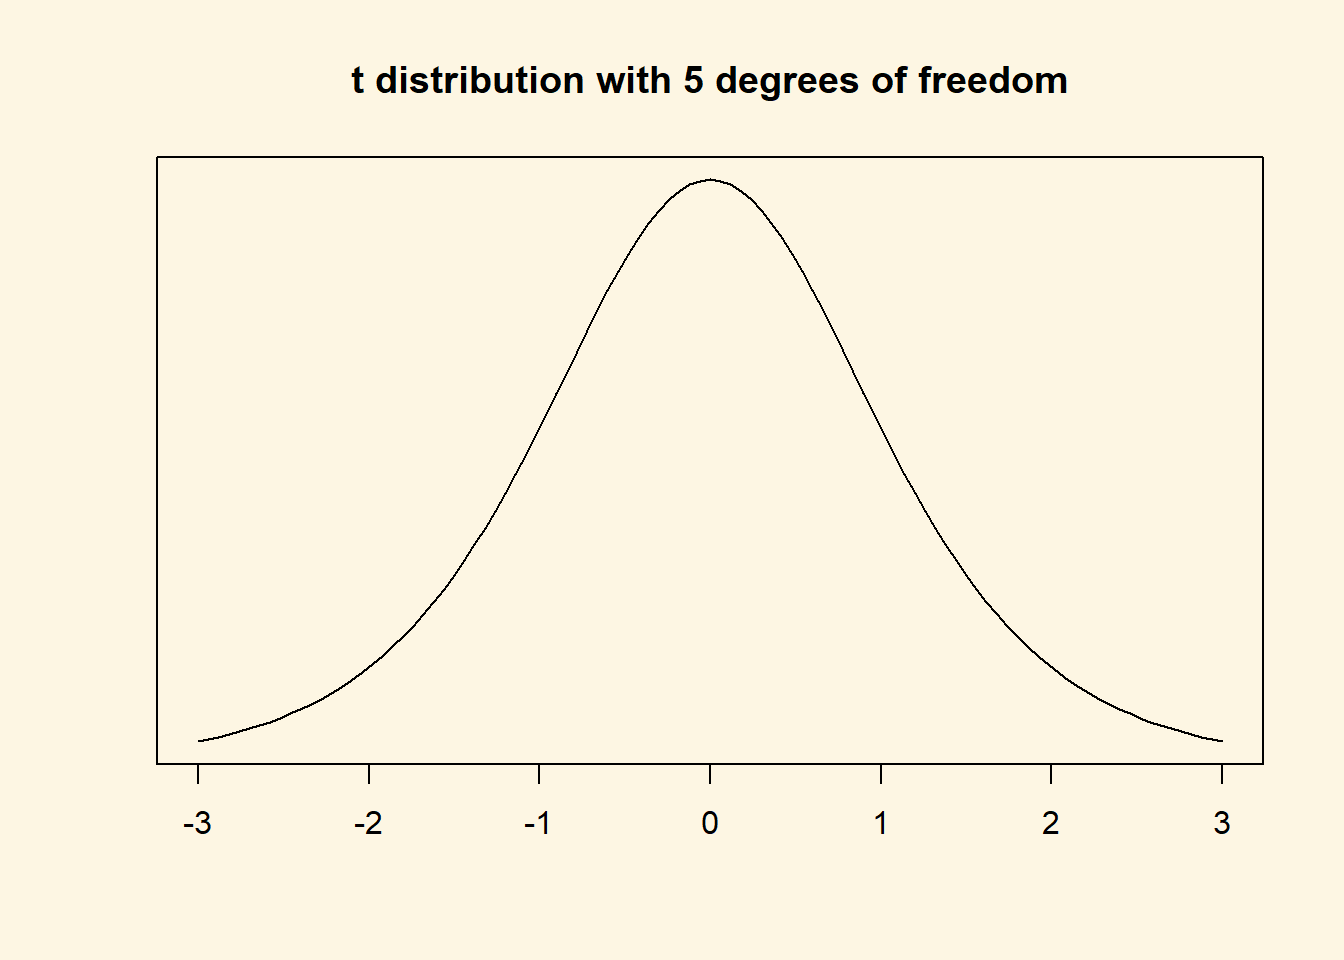
\includegraphics{statistics1_files/figure-latex/unnamed-chunk-189-1.pdf}

Although, it looks like a standard normal distribution, it is not. The t
with 5 degrees of freedom has fatter tails. We show this by overlaying
the t with a standard normal distribution.

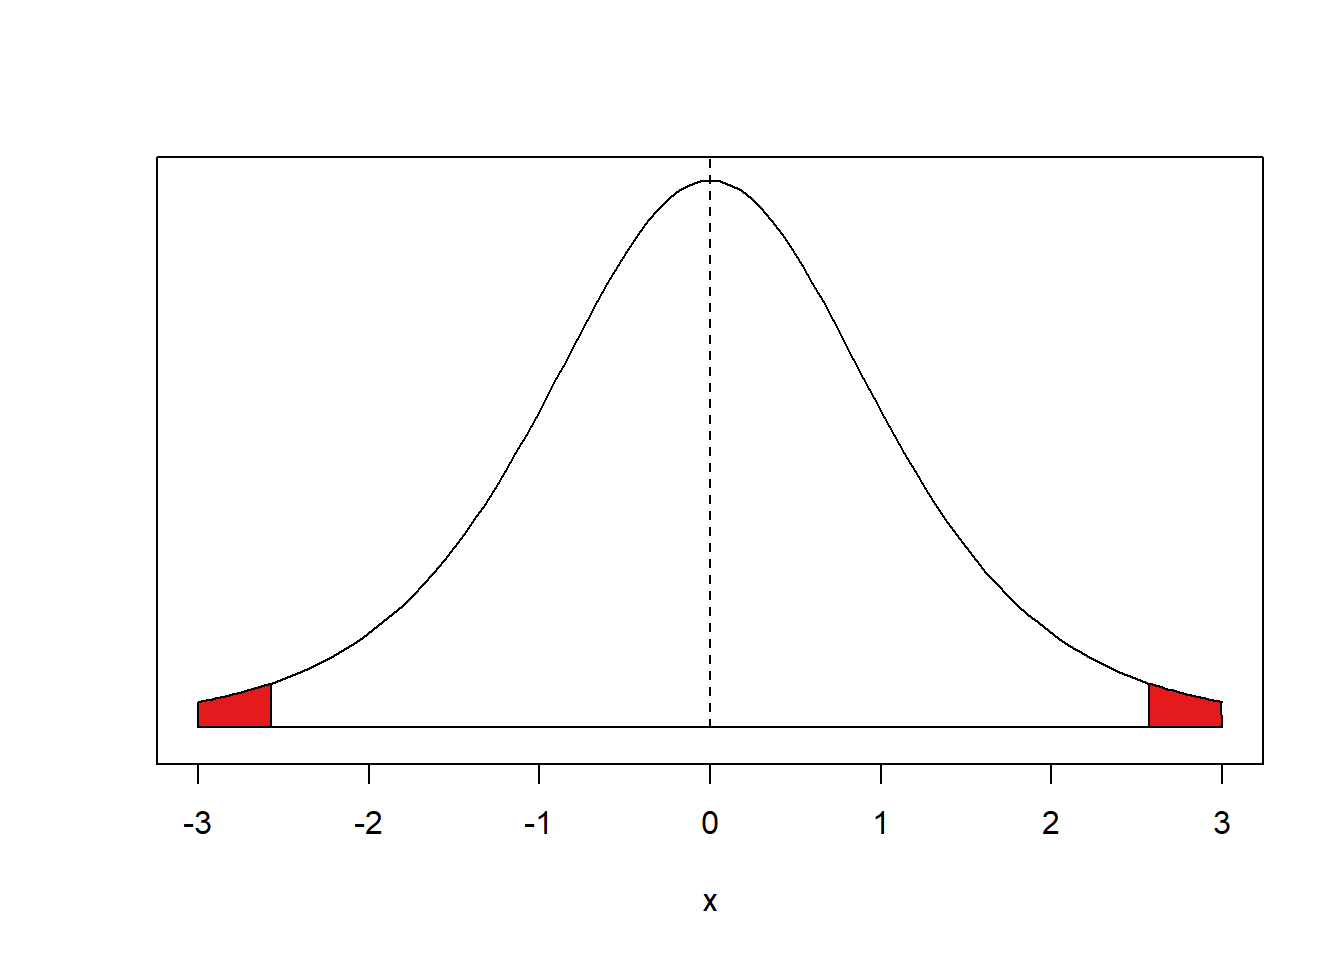
\includegraphics{statistics1_files/figure-latex/unnamed-chunk-190-1.pdf}

The red area is the difference between the standard normal distribution
and the t distribution with 5 degrees of freedom.

The tails are fatter and that means that the probabilities of getting a
value somewhere in the tails is larger. Lets calculate the critical
value for a t distribution with 5 degrees of freedom.

\begin{Shaded}
\begin{Highlighting}[]
\CommentTok{# value for cumulative probability 95 percent in the t distribution with 5 degrees of freedom}
\KeywordTok{qt}\NormalTok{(}\FloatTok{0.975}\NormalTok{, }\DataTypeTok{df =} \DecValTok{5}\NormalTok{)}
\end{Highlighting}
\end{Shaded}

\begin{verbatim}
[1] 2.570582
\end{verbatim}

See how much larger that value is than 1.96. Under a t distribution with
5 degrees of freedom 95 percent of the observations around the mean are
within the interval from negative 2.5705818 to positive 2.5705818.

Let's illustrate that.
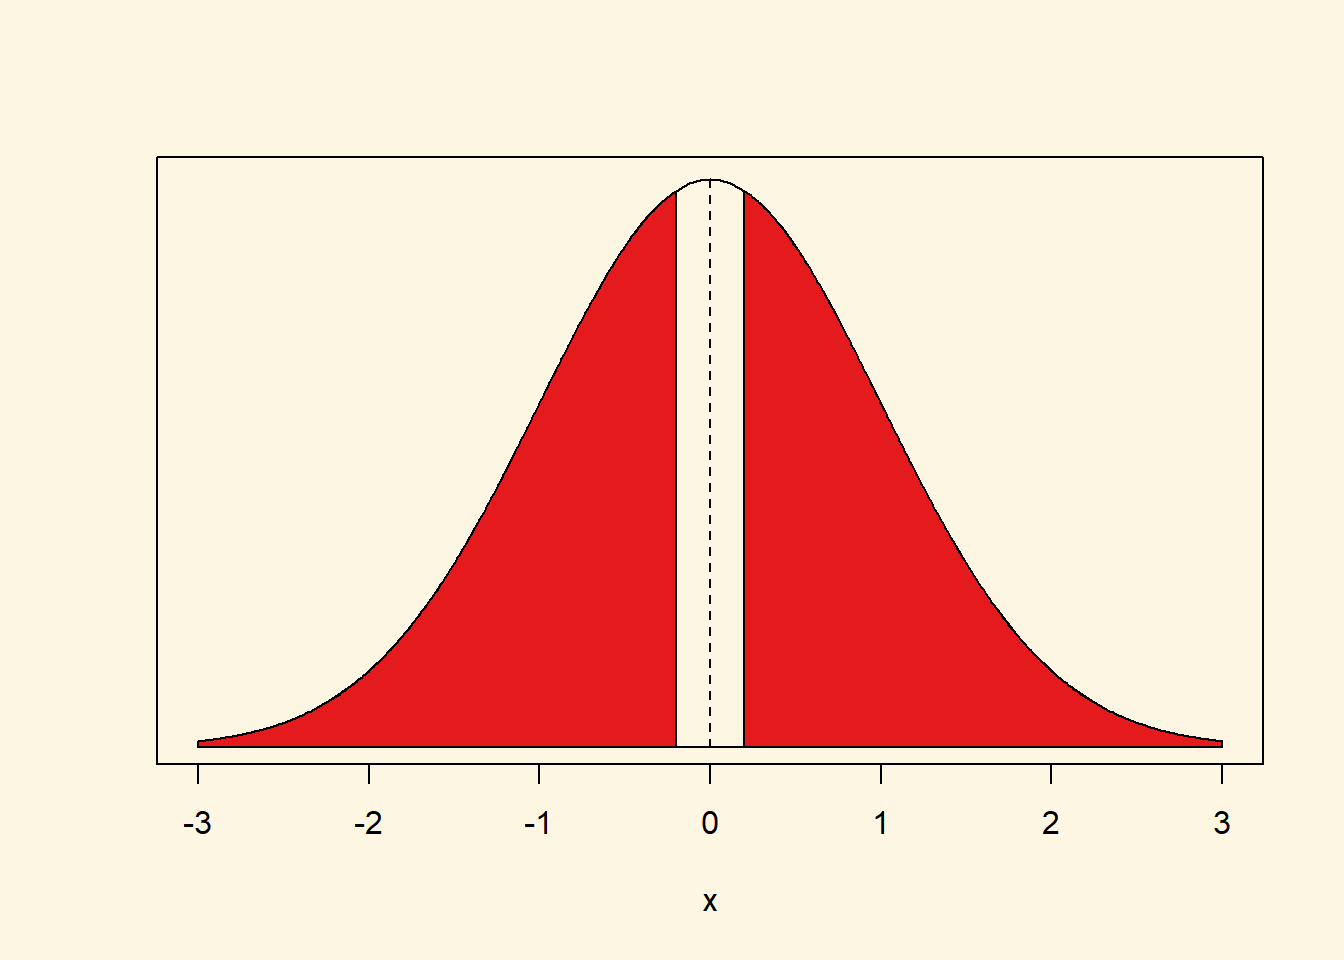
\includegraphics{statistics1_files/figure-latex/unnamed-chunk-192-1.pdf}

Remember the critical values for the t distribution are always more
extreme or similar to the critical values for the standard normal
distribution. If the t distribution has few degrees of freedom, the
critical values (for the same percentage area around the mean) are much
more extreme. If the t distribution has many degrees of freedom, the
critical values are very similar.

\subsubsection{T-test (difference in
means)}\label{t-test-difference-in-means}

We are interested in whether there is a difference in income between
countries that have an independent judiciary and countries that do not
have an independent judiciary. Put more formally, we are interested in
the difference between two conditional means. Recall that a conditional
mean is the mean in a subpopulation such as the mean of income given
that the country has a free judiciary (conditional mean 1).

The t-test is the appropriate test statistic. Our interval-level
dependent variable is \emph{wealth} which is GDP per capita taken from
the World Development Indicators of the World Bank. Our binary
independent variable is \emph{h\_j} which is 1 if a country has a free
judiciary and 0 otherwise.

Let's check the summary statistics of our dependent variable GDP per
captia using the
\href{https://www.rdocumentation.org/packages/base/versions/3.4.1/topics/summary}{\texttt{summary()}}.

\begin{Shaded}
\begin{Highlighting}[]
\KeywordTok{summary}\NormalTok{(world.data}\OperatorTok{$}\NormalTok{wealth)}
\end{Highlighting}
\end{Shaded}

\begin{verbatim}
   Min. 1st Qu.  Median    Mean 3rd Qu.    Max. 
  226.2  1768.0  5326.1 10184.1 12976.5 63686.7 
\end{verbatim}

Someone claims that countries with free judiciaries are usually richer
than countries with controlled judiciaries. From the output of the
\texttt{summary()} fucntion, we know that average wealth is
10184.0910395 US dollars across all countries---countries with and
without free judiciaries.

We use the \texttt{which()} function from last week again, to identify
the row-numbers of the countries in our dataset that have free
judiciaries. Use the \texttt{which()} to get the row numbers of
countries with free judiciaries.

\begin{Shaded}
\begin{Highlighting}[]
\KeywordTok{which}\NormalTok{(world.data}\OperatorTok{$}\NormalTok{h_j}\OperatorTok{==}\DecValTok{1}\NormalTok{)}
\end{Highlighting}
\end{Shaded}

\begin{verbatim}
 [1]   8   9  13  14  18  23  28  33  39  40  41  42  43  44  50  52  54
[18]  55  60  70  71  72  74  75  76  77  80  82  84  85  90  93  94 104
[35] 105 107 110 112 114 115 118 126 127 131 143 144 145 146 149 153 154
[52] 155 157 160 163 165 166 167 168 169 170 171 178
\end{verbatim}

Now, all we need is to index the dataset like we did last week. We
access the variable that we want (\emph{wealth}) with the dollar sign
and the rows in square brackets. Take the mean of \emph{wealth} for
countries with a free judiciary on your own.

\begin{Shaded}
\begin{Highlighting}[]
\KeywordTok{mean}\NormalTok{( world.data}\OperatorTok{$}\NormalTok{wealth[}\KeywordTok{which}\NormalTok{(world.data}\OperatorTok{$}\NormalTok{h_j}\OperatorTok{==}\DecValTok{1}\NormalTok{)])}
\end{Highlighting}
\end{Shaded}

\begin{verbatim}
[1] 17826.59
\end{verbatim}

Go ahead and find the mean per capita wealth of countries with
controlled judiciaries.

\begin{Shaded}
\begin{Highlighting}[]
\KeywordTok{mean}\NormalTok{( world.data}\OperatorTok{$}\NormalTok{wealth[}\KeywordTok{which}\NormalTok{(world.data}\OperatorTok{$}\NormalTok{h_j}\OperatorTok{==}\DecValTok{0}\NormalTok{)])}
\end{Highlighting}
\end{Shaded}

\begin{verbatim}
[1] 5884.882
\end{verbatim}

Finally, we run the t-test for the difference between two means.

\begin{Shaded}
\begin{Highlighting}[]
\CommentTok{# t.test for the difference between 2 means}
\KeywordTok{t.test}\NormalTok{(world.data}\OperatorTok{$}\NormalTok{wealth[}\KeywordTok{which}\NormalTok{(world.data}\OperatorTok{$}\NormalTok{h_j}\OperatorTok{==}\DecValTok{1}\NormalTok{)], }\CommentTok{# mean 1  }
\NormalTok{       world.data}\OperatorTok{$}\NormalTok{wealth[}\KeywordTok{which}\NormalTok{(world.data}\OperatorTok{$}\NormalTok{h_j}\OperatorTok{==}\DecValTok{0}\NormalTok{)], }\CommentTok{# mean 2}
       \DataTypeTok{mu =} \DecValTok{0}\NormalTok{, }\CommentTok{# difference under the null hypothesis}
       \DataTypeTok{alt =} \StringTok{"two.sided"}\NormalTok{,  }\CommentTok{# two sided test (difference in means could be smaller or larger than 0)}
       \DataTypeTok{conf =} \FloatTok{0.95}\NormalTok{) }\CommentTok{# confidence interval}
\end{Highlighting}
\end{Shaded}

\begin{verbatim}

    Welch Two Sample t-test

data:  world.data$wealth[which(world.data$h_j == 1)] and world.data$wealth[which(world.data$h_j == 0)]
t = 6.0094, df = 98.261, p-value = 0.00000003165
alternative hypothesis: true difference in means is not equal to 0
95 percent confidence interval:
  7998.36 15885.06
sample estimates:
mean of x mean of y 
17826.591  5884.882 
\end{verbatim}

Let's interpret the results you get from \texttt{t.test()}. The first
line tells us which groups we are comparing. In our example: Do
countries with independent judiciaries have different mean income levels
than countries without independent judiciaries?

In the following line you see the t-value, the degrees of freedom and
the p-value. Knowing the t-value and the degrees of freedom you can
check in a table on t distributions how likely you were to observe this
data, if the null-hypothesis was true. The p-value gives you this
probability directly. For example, a p-value of 0.02 would mean that the
probability of seeing this data given that there is no difference in
incomes between countries with and without independent judiciaries
\emph{in the population}, is 2\%. Here the p-value is much smaller than
this: 3.165e-08 = 0.00000003156!

In the next line you see the 95\% confidence interval because we
specified \texttt{conf=0.95}. If you were to take 100 samples and in
each you checked the means of the two groups, 95 times the difference in
means would be within the interval you see there.

At the very bottom you see the means of the dependent variable by the
two groups of the independent variable. These are the means that we
estimated above. In our example, you see the mean income levels in
countries were the executive has some control over the judiciary, and in
countries were the judiciary is independent.

Note that we are analysing a bi-variate relationship. The dependent
variable is \emph{wealth} and the independent variable is \emph{h\_j}.

Furthermroe, note that in the t test for the differences in means, the
degrees of freedom depend on the variances in each group. You do not
have to compute degrees of freedom for t tests for the differences in
means yourself in this class---just use the \texttt{t.test()} function.

\subsubsection{Estimating p values from t
values}\label{estimating-p-values-from-t-values}

Estimating the p value is the reverse of getting a critical value. We
have a t value and we want to know what the probability is to get such a
value or an even more extreme value.

Let's say that we have a t distribution with 5 degrees of freedom. We
estimated a t value of 2.9. What is the corresponding p value?

\begin{Shaded}
\begin{Highlighting}[]
\NormalTok{(}\DecValTok{1} \OperatorTok{-}\StringTok{ }\KeywordTok{pt}\NormalTok{(}\FloatTok{2.9}\NormalTok{, }\DataTypeTok{df =} \DecValTok{5}\NormalTok{)) }\OperatorTok{*}\DecValTok{2}
\end{Highlighting}
\end{Shaded}

\begin{verbatim}
[1] 0.0337907
\end{verbatim}

This is the probability of getting a t value of 2.9 or larger (or -2.9
or smaller) given that the null hypothesis is true.
\texttt{pt(2.9,\ df\ =\ 5)} is the cumulative probability of getting a t
value of 2.9 or smaller. But we want the probability of getting a value
that is as large (extreme) as 2.9 or as small as -2.9. Therefore, we do
\texttt{1\ -\ pt(2.9,\ df\ =\ 5)}. We multiply by 2 to get both tails
\texttt{(1\ -\ pt(2.9,\ df\ =\ 5))*2}. This is the probability of
getting a t value in the red tails of the distribution if the null
hypothesis was true.

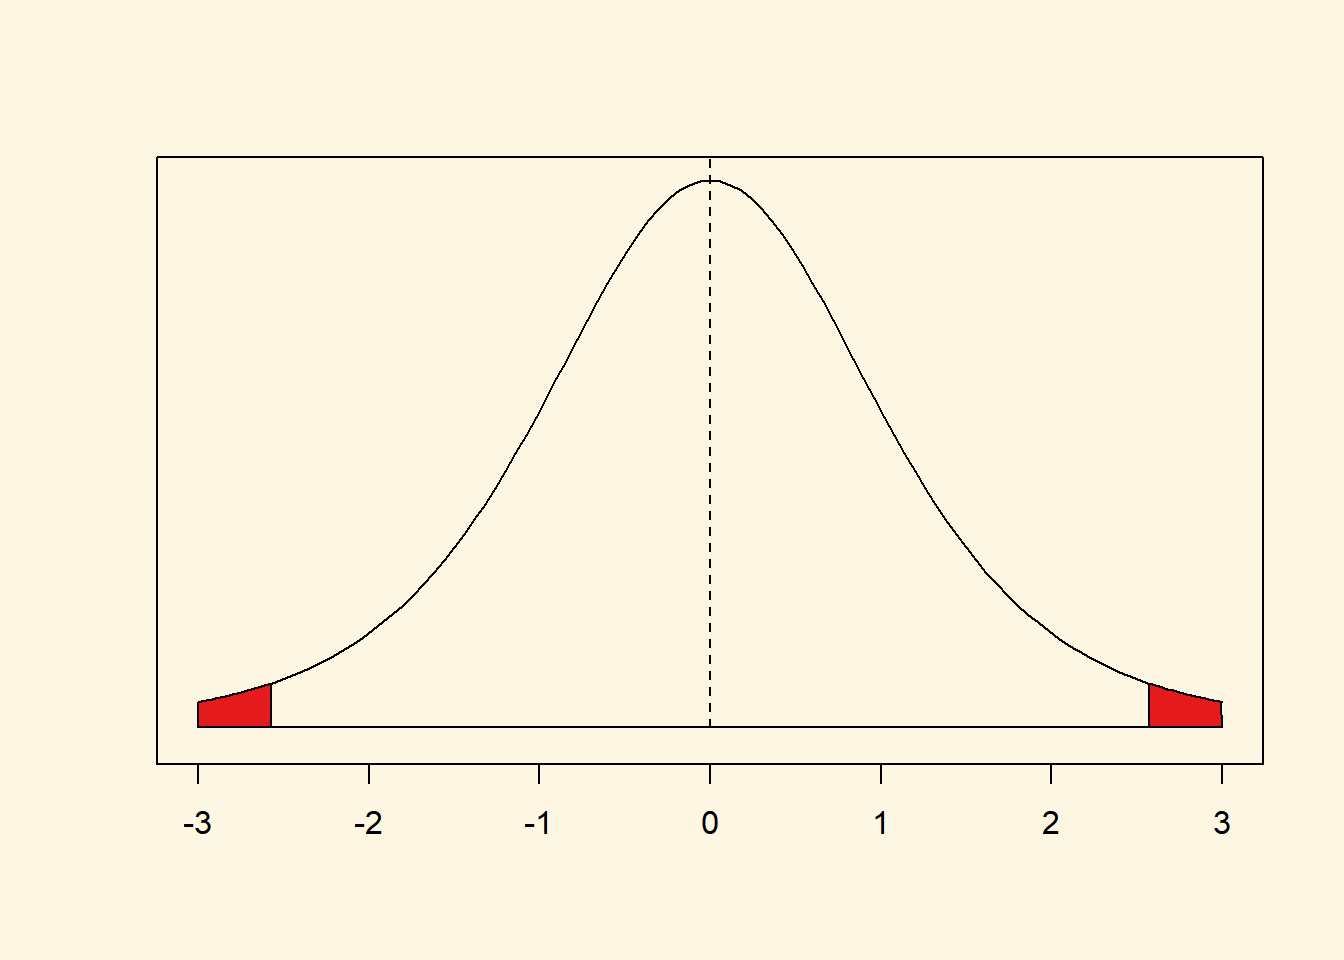
\includegraphics{statistics1_files/figure-latex/unnamed-chunk-199-1.pdf}

Clearly, the probability of getting such an extreme value (or something
larger) under the assumption that the null hypothesis is true is very
unlikely. The exact probability is \textasciitilde{}0.03 (3 percent).
We, therefore, think that the null hypothesis is false.

Let's estimate the p value in a normal distribution (it's actually
better to always use the t distribution but the difference is negligible
if the t distribution has many degrees of freedom).

Let's take our earlier example where we had estimated a t value of
0.1995059. Our friend claimed world income is 10 000 per capita on
average and we estimated something slightly larger.

Let's check what the exact p value is in a normal distribution given a t
value of 0.1995059.

\begin{Shaded}
\begin{Highlighting}[]
\NormalTok{(}\DecValTok{1} \OperatorTok{-}\StringTok{ }\KeywordTok{pnorm}\NormalTok{(}\FloatTok{0.1995059}\NormalTok{))}\OperatorTok{*}\DecValTok{2}
\end{Highlighting}
\end{Shaded}

\begin{verbatim}
[1] 0.841867
\end{verbatim}

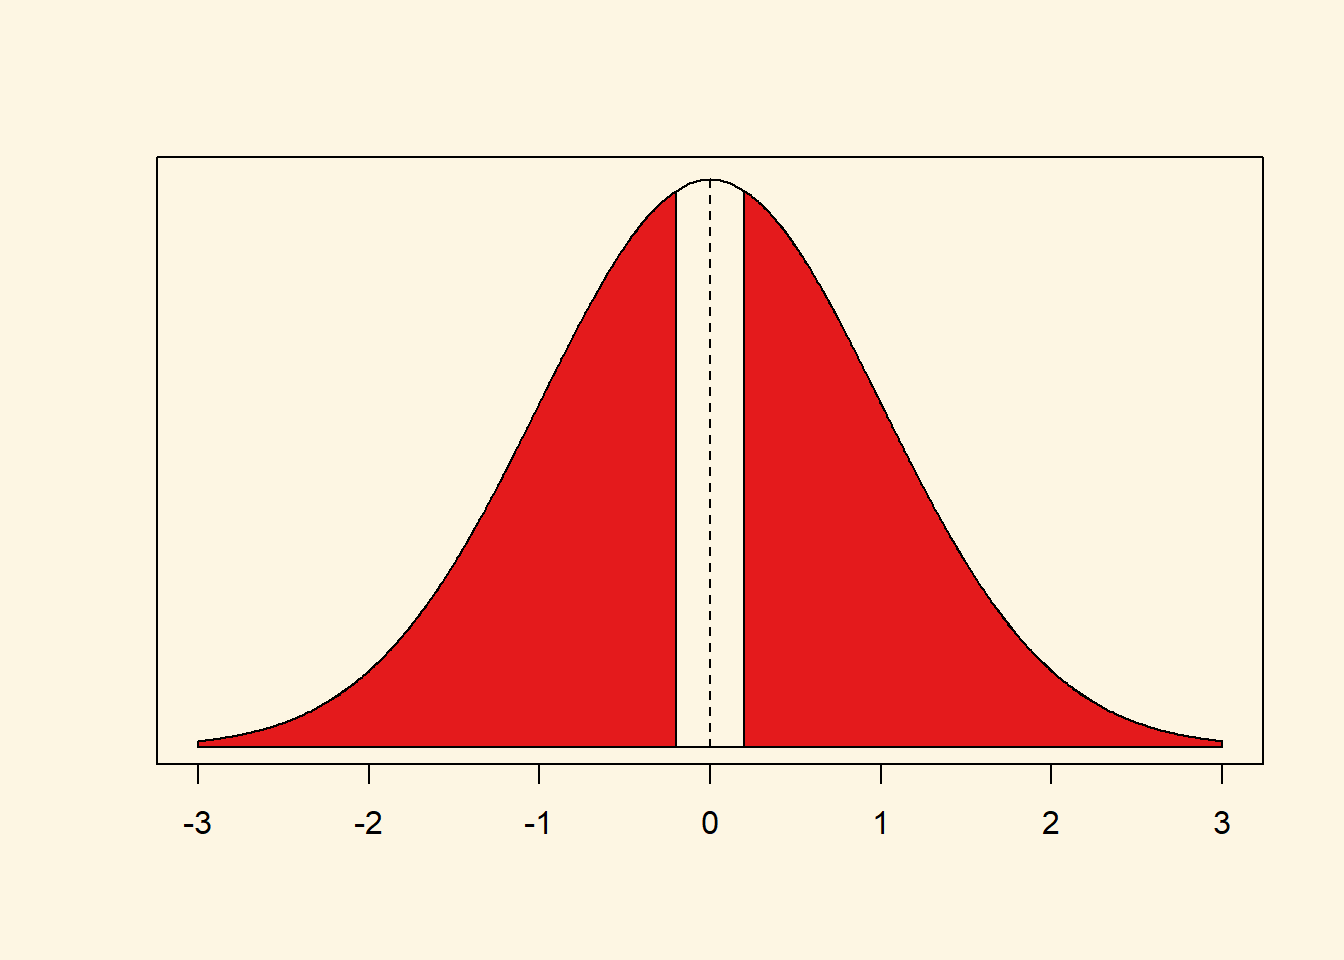
\includegraphics{statistics1_files/figure-latex/unnamed-chunk-201-1.pdf}

Clearly, it was not very unlikely to find a t value of 0.1995059 (that's
the absolute value, i.e., a t value of negative or postive 0.1995059)
under the assumption that the null hypothesis is true. Therefore, we
cannot reject the null. The probability is 0.84 (84 percent)---highly
likely.

\subsubsection{Exercises}\label{exercises-3}

\begin{enumerate}
\def\labelenumi{\arabic{enumi}.}
\tightlist
\item
  Create a new file called ``assignment4.R'' in your
  \texttt{statistics\ 1} folder and write all the solutions in it.
\item
  Turn former colonies into a factor variable and choose appropriate
  labels.
\item
  How many countries were former colonies? How many were not?
\item
  Find the means of political stability in countries that (1) were
  former colonies, (2) were not former colonies.
\item
  Is the the difference in means statistically significant?
\item
  In layman's terms, are countries which were former colonies more or
  less stable than those that were not?
\item
  How about if we choose an alpha level of 0.01?
\item
  What is the level of measurement of the United Nations Development
  index variable \texttt{undp\_hdi}?
\item
  Check the claim that its true population mean is 0.85.
\item
  Calculate the t statistic.
\item
  Calculate the p value.
\item
  Construct a confidence interval around your mean estimate.
\item
  Discuss your findings in terms of the original claim. Interpret the t
  value, the p value, and the confidence interval.
\item
  Compute the critical value for the 99.9 percent confidence interval in
  a standard normal distribution.
\item
  Compute the critical value for the 99.9 percent confidence interval in
  a t distribution with 11 degrees of freedom.
\item
  Save the script that includes all previous tasks.
\item
  Source your script, i.e.~run the entire script all at once without
  error message.
\end{enumerate}

\subsubsection{Optional Exercises that require reading Extra Info
below}\label{optional-exercises-that-require-reading-extra-info-below}

\begin{enumerate}
\def\labelenumi{\arabic{enumi}.}
\setcounter{enumi}{17}
\tightlist
\item
  Create a scatter plot with latitude on the x-axis and political
  stability on the y-axis.
\item
  What is the correlation coefficient of political stability and
  latitude?
\item
  If we move away from the equator, how does political stability change?
\item
  Does it matter whether we go north or south from the equator?
\end{enumerate}

\subsubsection{Advanced Exercises}\label{advanced-exercises}

\begin{enumerate}
\def\labelenumi{\arabic{enumi}.}
\setcounter{enumi}{21}
\tightlist
\item
  Calculate the numerical difference in means (political stability
  conditional on colonialization) using the \texttt{means()} function.
\item
  Calculate the standard deviation of the difference in means (hint:
  using just the \texttt{sd()} function is incorrect in this context).
\item
  Is the difference in means more than 1.96 standard deviations away
  from zero? Interpret the result.
\item
  We claim the difference in means in terms of political stability
  between countries that were former colonies and those that were not is
  0.3. Check this hypothesis.
\item
  An angry citizen who wants to defund the Department of International
  Development (DFID) claims that countries that were former colonies
  have reached 75\% of the level of wealth of countries that were not
  colonised. Check this claim.
\end{enumerate}

\subsubsection{Extra Info}\label{extra-info}

When we want to get an idea about how two continuous variables change
together, the best way is to plot the relationship in a scatterplot. A
scatterplot means that we plot one continuous variable on the x-axis and
the other on the y-axis. Here, we illustrate the relation between the
human development index \texttt{undp\_hdi} and control of corruption
\texttt{wbgi\_cce}.

\begin{Shaded}
\begin{Highlighting}[]
\CommentTok{# scatterplot}
\KeywordTok{plot}\NormalTok{(world.data}\OperatorTok{$}\NormalTok{undp_hdi }\OperatorTok{~}\StringTok{ }\NormalTok{world.data}\OperatorTok{$}\NormalTok{wbgi_cce,}
  \DataTypeTok{xlim =} \KeywordTok{c}\NormalTok{(}\DataTypeTok{xmin =} \OperatorTok{-}\DecValTok{2}\NormalTok{, }\DataTypeTok{xmax =} \DecValTok{3}\NormalTok{),}
  \DataTypeTok{ylim =} \KeywordTok{c}\NormalTok{(}\DataTypeTok{ymin =} \DecValTok{0}\NormalTok{, }\DataTypeTok{ymax =} \DecValTok{1}\NormalTok{),}
  \DataTypeTok{frame =} \OtherTok{FALSE}\NormalTok{,}
  \DataTypeTok{xlab =} \StringTok{"World Bank Control of Corruption Index"}\NormalTok{,}
  \DataTypeTok{ylab =} \StringTok{"UNDP Human Development Index"}\NormalTok{,}
  \DataTypeTok{main =} \StringTok{"Relationship b/w Quality of Institutions and Quality of Life"}
\NormalTok{  )}
\end{Highlighting}
\end{Shaded}

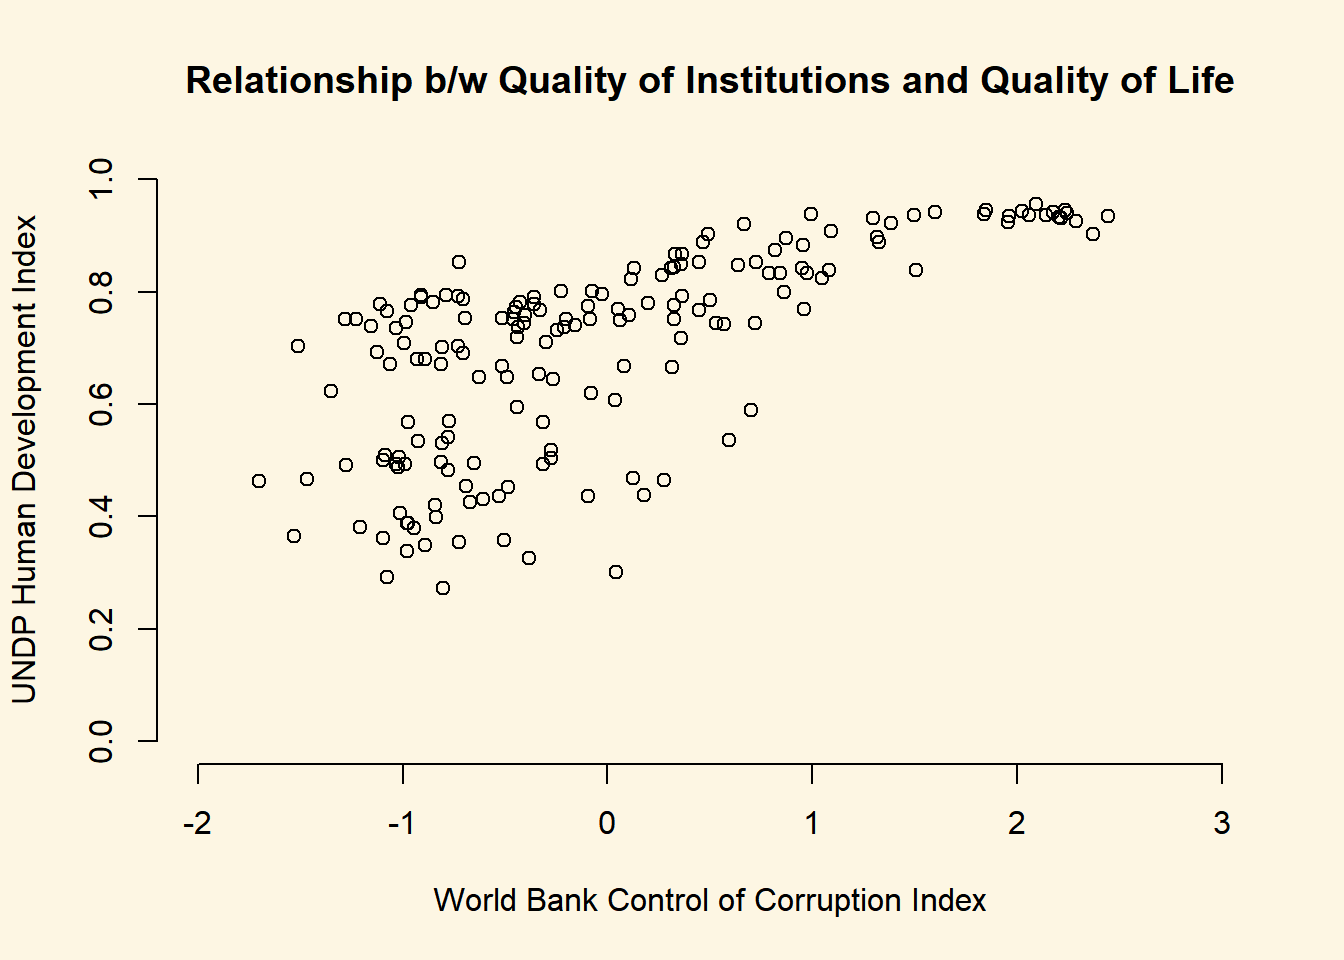
\includegraphics{statistics1_files/figure-latex/unnamed-chunk-202-1.pdf}

Sometimes people will report the correlation coefficient which is a
measure of linear association and ranges from -1 to +1. Where -1 means
perfect negative relation, 0 means no relation and +1 means perfect
positive relation. The correlation coefficient is commonly used as as
summary statistic. It's disadvantage is that you cannot see the
non-linear relations which can using a scatterplot.

We take the correlation coefficient like so:

\begin{Shaded}
\begin{Highlighting}[]
\KeywordTok{cor}\NormalTok{(}\DataTypeTok{y =}\NormalTok{ world.data}\OperatorTok{$}\NormalTok{undp_hdi, }\DataTypeTok{x =}\NormalTok{ world.data}\OperatorTok{$}\NormalTok{wbgi_cce, }\DataTypeTok{use =} \StringTok{"complete.obs"}\NormalTok{)}
\end{Highlighting}
\end{Shaded}

\begin{verbatim}
[1] 0.6813353
\end{verbatim}

\begin{longtable}[]{@{}ll@{}}
\toprule
\begin{minipage}[b]{0.12\columnwidth}\raggedright\strut
Argument\strut
\end{minipage} & \begin{minipage}[b]{0.78\columnwidth}\raggedright\strut
Description\strut
\end{minipage}\tabularnewline
\midrule
\endhead
\begin{minipage}[t]{0.12\columnwidth}\raggedright\strut
\texttt{x}\strut
\end{minipage} & \begin{minipage}[t]{0.78\columnwidth}\raggedright\strut
The x variable that you want to correlate.\strut
\end{minipage}\tabularnewline
\begin{minipage}[t]{0.12\columnwidth}\raggedright\strut
\texttt{y}\strut
\end{minipage} & \begin{minipage}[t]{0.78\columnwidth}\raggedright\strut
The y variable that you want to correlate.\strut
\end{minipage}\tabularnewline
\begin{minipage}[t]{0.12\columnwidth}\raggedright\strut
\texttt{use}\strut
\end{minipage} & \begin{minipage}[t]{0.78\columnwidth}\raggedright\strut
How R should handle missing values. \texttt{use="complete.obs"} will use
only those rows where neither \texttt{x} nor \texttt{y} is
missing.\strut
\end{minipage}\tabularnewline
\bottomrule
\end{longtable}

\subsection{Solutions}\label{solutions-3}

\paragraph{Exercise 2}\label{exercise-2-2}

Turn former colonies into a factor variable and choose appropriate
labels.

First, we load the dataset and then factorise the former colonies
variable.

\begin{Shaded}
\begin{Highlighting}[]
\CommentTok{# load data}
\NormalTok{world.data <-}\StringTok{ }\KeywordTok{read.csv}\NormalTok{(}\StringTok{"QoG2012.csv"}\NormalTok{)}

\CommentTok{# turn variable into a factor}
\NormalTok{world.data}\OperatorTok{$}\NormalTok{former_col <-}\StringTok{ }\KeywordTok{factor}\NormalTok{(world.data}\OperatorTok{$}\NormalTok{former_col, }\DataTypeTok{labels =} \KeywordTok{c}\NormalTok{(}\StringTok{"not colonised"}\NormalTok{, }\StringTok{"was colonised"}\NormalTok{), }\DataTypeTok{levels =} \KeywordTok{c}\NormalTok{(}\DecValTok{0}\NormalTok{,}\DecValTok{1}\NormalTok{))}
\end{Highlighting}
\end{Shaded}

\paragraph{Exercise 3}\label{exercise-3-3}

How many countries were former colonies? How many were not?

We can get the numbers from a frequency table.

\begin{Shaded}
\begin{Highlighting}[]
\KeywordTok{table}\NormalTok{(world.data}\OperatorTok{$}\NormalTok{former_col)}
\end{Highlighting}
\end{Shaded}

\begin{verbatim}

not colonised was colonised 
           72           122 
\end{verbatim}

122 countries were victims of colonialization.

\paragraph{Exercise 4}\label{exercise-4-3}

Find the means of political stability in countries that (1) were former
colonies, (2) were not former colonies.

We use the mean function to get the mean of political stability and
subset for the groups of countries using the square brackets.

\begin{Shaded}
\begin{Highlighting}[]
\CommentTok{# mean of political stability in countries that were not colonised}
\KeywordTok{mean}\NormalTok{(world.data}\OperatorTok{$}\NormalTok{wbgi_pse[world.data}\OperatorTok{$}\NormalTok{former_col}\OperatorTok{==}\StringTok{"not colonised"}\NormalTok{])}
\end{Highlighting}
\end{Shaded}

\begin{verbatim}
[1] 0.2858409
\end{verbatim}

\begin{Shaded}
\begin{Highlighting}[]
\CommentTok{# mean of political stability in countries that were colonised}
\KeywordTok{mean}\NormalTok{(world.data}\OperatorTok{$}\NormalTok{wbgi_pse[world.data}\OperatorTok{$}\NormalTok{former_col}\OperatorTok{==}\StringTok{"was colonised"}\NormalTok{])}
\end{Highlighting}
\end{Shaded}

\begin{verbatim}
[1] -0.231612
\end{verbatim}

The average level of political stability in countries that were not
colonised is 0.2858409. Mean political stability in countries that were
colonised is -0.231612. The variable political stability
\texttt{wbgi\_pse} is an index. Larger values correspond with more
political stability. We see that political stability is higher in
countries that were not colonised.

Looking at this difference, we might conclude that the legacy of
colonialism is still visible today and manifests itself in lower
political stability. Let's investigate further to see whether the
difference in means is statistically significant.

\paragraph{Exercise 5}\label{exercise-5-3}

Is the the difference in means statistically significant?

Let's first compute the difference in means. We call it \texttt{fd}
here. We could name it anything but \texttt{fd} is shorthand for first
difference. Differences between two means are sometimes referred to as
first differences.

\begin{Shaded}
\begin{Highlighting}[]
\NormalTok{fd <-}\StringTok{ }\KeywordTok{mean}\NormalTok{(world.data}\OperatorTok{$}\NormalTok{wbgi_pse[world.data}\OperatorTok{$}\NormalTok{former_col}\OperatorTok{==}\StringTok{"not colonised"}\NormalTok{]) }\OperatorTok{-}\StringTok{ }\KeywordTok{mean}\NormalTok{(world.data}\OperatorTok{$}\NormalTok{wbgi_pse[world.data}\OperatorTok{$}\NormalTok{former_col}\OperatorTok{==}\StringTok{"was colonised"}\NormalTok{])}
\NormalTok{fd}
\end{Highlighting}
\end{Shaded}

\begin{verbatim}
[1] 0.5174529
\end{verbatim}

The numerical difference is 0.5174529. Is this difference small or
large? That is difficult to say because the variable is not measured in
intuitive units (income in dollars is an example of a variable that is
measured in intuitive units).

Let's look at the variable a little closer to understand this difference
in substantive terms.

\begin{Shaded}
\begin{Highlighting}[]
\CommentTok{# the range}
\KeywordTok{range}\NormalTok{(world.data}\OperatorTok{$}\NormalTok{wbgi_pse)}
\end{Highlighting}
\end{Shaded}

\begin{verbatim}
[1] -2.467461  1.675609
\end{verbatim}

\begin{Shaded}
\begin{Highlighting}[]
\CommentTok{# the distance from the minimum to the maximum value}
\KeywordTok{diff}\NormalTok{(}\KeywordTok{range}\NormalTok{(world.data}\OperatorTok{$}\NormalTok{wbgi_pse))}
\end{Highlighting}
\end{Shaded}

\begin{verbatim}
[1] 4.14307
\end{verbatim}

\begin{Shaded}
\begin{Highlighting}[]
\CommentTok{# the difference in means as percentage change over the range of the variable}
\NormalTok{fd }\OperatorTok{/}\StringTok{ }\KeywordTok{diff}\NormalTok{(}\KeywordTok{range}\NormalTok{(world.data}\OperatorTok{$}\NormalTok{wbgi_pse))}
\end{Highlighting}
\end{Shaded}

\begin{verbatim}
[1] 0.124896
\end{verbatim}

Doing the above was not necessary to answer the question but it is
helpful to understand the variable in substantive terms. The difference
in means is 0.5174529. That constitutes 0.124896 (12\%) of the range of
the variable. So the difference in political stability between countries
that were colonies and those that were not is large.

We now test whether the difference is statistically significant using
the t-test.

\begin{Shaded}
\begin{Highlighting}[]
\CommentTok{# t test for difference in means}
\KeywordTok{t.test}\NormalTok{(world.data}\OperatorTok{$}\NormalTok{wbgi_pse[world.data}\OperatorTok{$}\NormalTok{former_col }\OperatorTok{==}\StringTok{ "not colonised"}\NormalTok{],}
\NormalTok{       world.data}\OperatorTok{$}\NormalTok{wbgi_pse[world.data}\OperatorTok{$}\NormalTok{former_col }\OperatorTok{==}\StringTok{ "was colonised"}\NormalTok{], }
       \DataTypeTok{mu =} \DecValTok{0}\NormalTok{, }\DataTypeTok{alt =} \StringTok{"two.sided"}\NormalTok{)}
\end{Highlighting}
\end{Shaded}

\begin{verbatim}

    Welch Two Sample t-test

data:  world.data$wbgi_pse[world.data$former_col == "not colonised"] and world.data$wbgi_pse[world.data$former_col == "was colonised"]
t = 3.4674, df = 139.35, p-value = 0.0006992
alternative hypothesis: true difference in means is not equal to 0
95 percent confidence interval:
 0.2224004 0.8125053
sample estimates:
 mean of x  mean of y 
 0.2858409 -0.2316120 
\end{verbatim}

As we can see, the difference is not only large it is also a noticeable
systematic difference. The p value is small. Smaller than the
conventional alpha level of 0.05. We can also look at the confidence
interval which ranges from 0.2224004 to 0.8125053. So, if we were to
repeatedly sample, the confidence interval of each sample would include
the true population mean \(95\%\) of the time. Or more intuitively, we
are \(95\%\) confident that the average population level of political
stability is within our interval.

\paragraph{Exercise 6}\label{exercise-6-3}

In layman's terms, are countries which were former colonies more or less
stable than those that were not?

The results from the t-test show that countries that were colonies are
less stable than those that were not. The difference is large and
systematic.

\paragraph{Exercise 7}\label{exercise-7-2}

How about if we choose an alpha level of 0.01?

The p-value is 0.0006992. That is smaller than an alpha level of 0.01 as
well. Therefore, picking an alpha level of 0.01 does not change our
results.

\paragraph{Exercise 8}\label{exercise-8-3}

What is the level of measurement of the United Nations Development index
variable \texttt{undp\_hdi}?

We googled
\href{http://hdr.undp.org/en/content/human-development-index-hdi}{united
nations human development index} and found that the variable is a
composite index of three key dimensions: a long and healthy life, being
knowledgeable and having a decent standard of living. The description
goes on to tell us how the dimensions are measured and that the index is
the geometric average of the components. The variable is, therefore,
continuous.

\paragraph{Exercise 9}\label{exercise-9-2}

Check the claim that its true population mean is 0.85.

Let's estimate the mean from our sample

\begin{Shaded}
\begin{Highlighting}[]
\KeywordTok{summary}\NormalTok{(world.data}\OperatorTok{$}\NormalTok{undp_hdi)}
\end{Highlighting}
\end{Shaded}

\begin{verbatim}
   Min. 1st Qu.  Median    Mean 3rd Qu.    Max.    NA's 
 0.2730  0.5390  0.7510  0.6982  0.8335  0.9560      19 
\end{verbatim}

Our estimate is 0.69824. The claim is that it is 0.85.

Null hypothesis: The true population mean of the human development index
is: 0.85. Alternative hypothesis: The true population mean is different
from 0.85.

We pick an alpha level of 0.05 for our test.

\begin{Shaded}
\begin{Highlighting}[]
\KeywordTok{t.test}\NormalTok{(world.data}\OperatorTok{$}\NormalTok{undp_hdi, }\DataTypeTok{mu =} \FloatTok{0.85}\NormalTok{, }\DataTypeTok{alt =} \StringTok{"two.sided"}\NormalTok{)}
\end{Highlighting}
\end{Shaded}

\begin{verbatim}

    One Sample t-test

data:  world.data$undp_hdi
t = -11.139, df = 174, p-value < 0.00000000000000022
alternative hypothesis: true mean is not equal to 0.85
95 percent confidence interval:
 0.6713502 0.7251298
sample estimates:
mean of x 
  0.69824 
\end{verbatim}

The p-value is lower than 0.05 and hence we reject the null hypothesis
(hdi is 0.85). Looking at our confidence interval, we expect that if we
were to repeatedly sample, the population mean would fall into the
interval 0.6713502 to 0.7251298 \(95\%\) of the time.

\paragraph{Exercise 10}\label{exercise-10-2}

Calculate the t statistic.

We could take the t statistic from the t test above. But we are going
through the individual steps here.

From the \texttt{summary()} function above, we know that there are 19
missings on the variable which we drop. We create a copy of our data in
the original state and then drop the missing rows from
\textbf{world.data}.

\begin{Shaded}
\begin{Highlighting}[]
\CommentTok{# copy of world data}
\NormalTok{world.data.full <-}\StringTok{ }\NormalTok{world.data}

\CommentTok{# drop missings on undp_hdi}
\NormalTok{world.data <-}\StringTok{ }\NormalTok{world.data[ }\OperatorTok{!}\KeywordTok{is.na}\NormalTok{(world.data}\OperatorTok{$}\NormalTok{undp_hdi),  ]}
\end{Highlighting}
\end{Shaded}

Step 1: We get the number of observations.

\begin{Shaded}
\begin{Highlighting}[]
\NormalTok{n <-}\StringTok{ }\KeywordTok{length}\NormalTok{(world.data}\OperatorTok{$}\NormalTok{undp_hdi)}
\NormalTok{n}
\end{Highlighting}
\end{Shaded}

\begin{verbatim}
[1] 175
\end{verbatim}

Step 2: We calculate the standard variation of the random variable
\texttt{undp\_hdi}.

\begin{Shaded}
\begin{Highlighting}[]
\CommentTok{# sample standard deviation of undp_hdi}
\NormalTok{sd_hdi <-}\StringTok{ }\KeywordTok{sd}\NormalTok{(world.data}\OperatorTok{$}\NormalTok{undp_hdi)}
\end{Highlighting}
\end{Shaded}

Step 3: We calculate the standard error of the mean which is:

\[ SE({\bar{Y}}) = \frac{ s_{Y}}  { \sqrt{n}} \]

\begin{Shaded}
\begin{Highlighting}[]
\CommentTok{# standard error of the mean of undp_hdi}
\NormalTok{se.y_bar <-}\StringTok{ }\NormalTok{sd_hdi }\OperatorTok{/}\StringTok{ }\KeywordTok{sqrt}\NormalTok{(n)}
\end{Highlighting}
\end{Shaded}

Step 4: We compute the t-statistic as the difference between our
estimated mean and the mean under null and then divide by the standard
error of the estimated mean.

\[ t = \frac{ \bar{Y} - \mu_{0}}  { SE({\bar{Y}}) } \]

Note: By dividing by the standard error of the estimated mean, we are
making the difference of the means (our estimated mean - the mean under
the null), free of the units that the variables were measured in. The
t-value is the difference of the means, were its units are standard
deviations.

The t-value follows a t-distribution with n-1 (174) degrees of freedom.
It is well approximated by a standard normal distribution.

\begin{Shaded}
\begin{Highlighting}[]
\NormalTok{hdi_mean <-}\StringTok{ }\KeywordTok{mean}\NormalTok{(world.data}\OperatorTok{$}\NormalTok{undp_hdi)}
\NormalTok{t.statistic <-}\StringTok{ }\NormalTok{( hdi_mean }\OperatorTok{-}\StringTok{ }\FloatTok{0.85}\NormalTok{ ) }\OperatorTok{/}\StringTok{ }\NormalTok{se.y_bar }
\NormalTok{t.statistic}
\end{Highlighting}
\end{Shaded}

\begin{verbatim}
[1] -11.13908
\end{verbatim}

The t.statistic is -11.13908. Given that this t statistic follows a
standard normal distribution approximately (because the sample is
large), we would reject the null hypothesis if the t-value is more than
1.96 standard deviations away from 0. This t-value is 11 standard
deviations away from zero. The t-value is very far in the tails of the
distribution. It is very unlikely that we would have estimated the mean
that we did estimate (0.69824) if the population average of HDI really
was 0.85.

We can reject the null hypothesis.

\paragraph{Exercise 11}\label{exercise-11-1}

Calculate the p value.

We have the t statistic already. We will follow the steps to get the p
value. But first, take a look at what the distribution of our t
statistic looks like. Our t statistic is -11.13908. This is very very
far in the left tail.

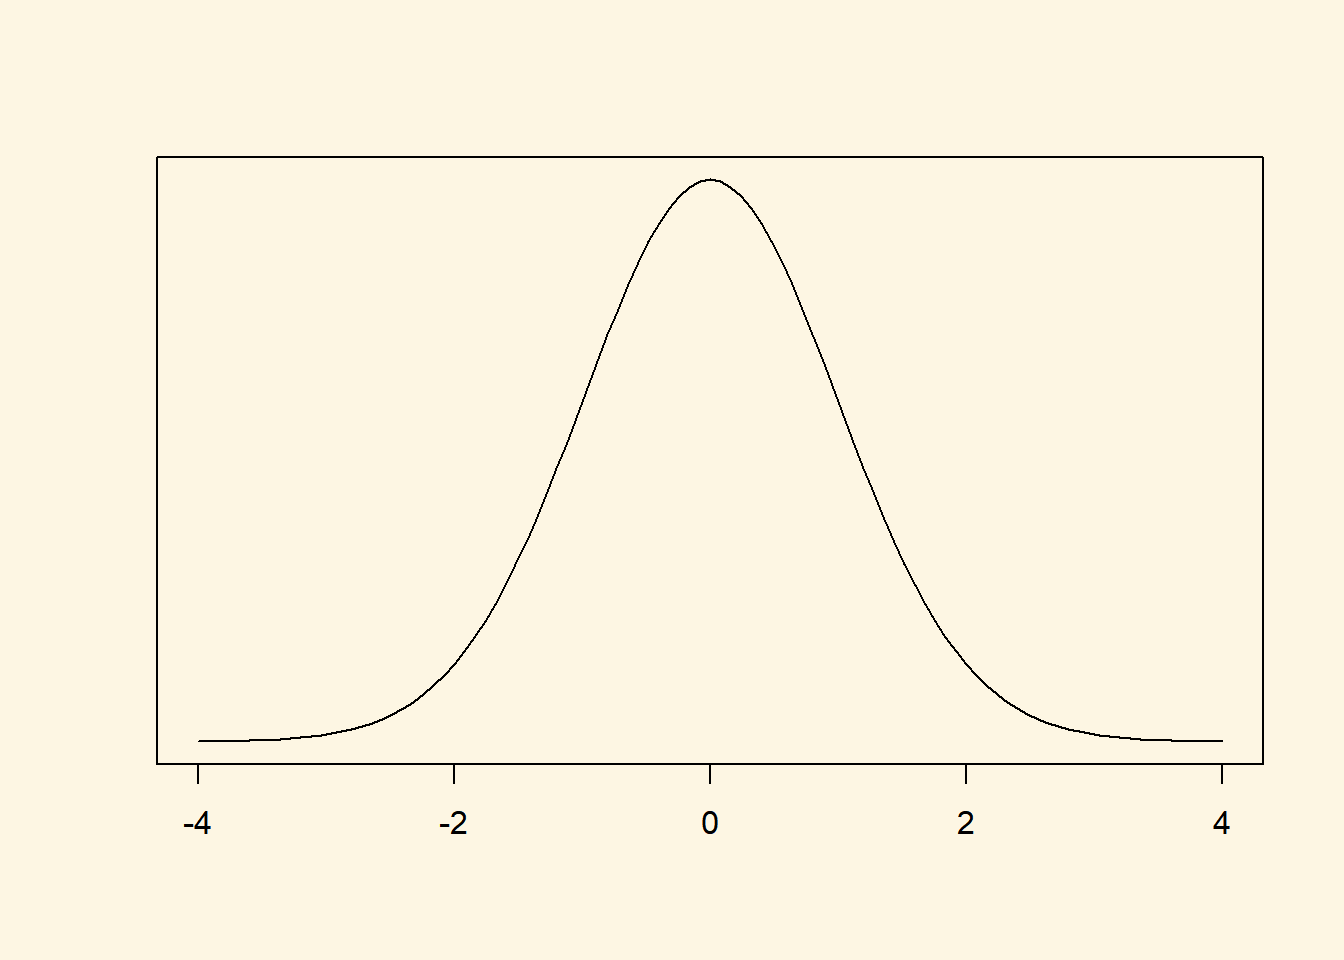
\includegraphics{statistics1_files/figure-latex/unnamed-chunk-219-1.pdf}

Step 1: We compute the cumulative probability to get our t-value or
something smaller from this distribution.

\begin{Shaded}
\begin{Highlighting}[]
\NormalTok{cum.prob.at.least.t <-}\StringTok{ }\KeywordTok{pt}\NormalTok{(t.statistic, }\DataTypeTok{df =}\NormalTok{ (n}\OperatorTok{-}\DecValTok{1}\NormalTok{) )}
\NormalTok{cum.prob.at.least.t}
\end{Highlighting}
\end{Shaded}

\begin{verbatim}
[1] 0.0000000000000000000002127538
\end{verbatim}

Notice that our t value is negative. By calculating the probability to
get a t-value as large or smaller, we alredy have the proability that we
see a t value like this in the left tail. We are conducting a two-sided
test. Therefore, we want the proability in the right tail as well, i.e.,
to see a t value that is 11.139 or larger. So in the next step we take
the probability we got times 2.

\begin{Shaded}
\begin{Highlighting}[]
\NormalTok{cum.prob.at.least.t }\OperatorTok{*}\StringTok{ }\DecValTok{2}
\end{Highlighting}
\end{Shaded}

\begin{verbatim}
[1] 0.0000000000000000000004255075
\end{verbatim}

The p value is extremely small. In fact, it is so small that the t-test
did not report the correct p value either but simply stated that the p
value is smaller than 2.2e-16.

Notice also that in the seminar we calucated
\texttt{(1\ -\ pt(t.statistic,\ df\ =\ n-1))*2}. This was because our t
value was positive in the seminar. Here it is negative. Here in this
task, we could have calculated
\texttt{(1\ -\ pt(abs(t.statistic),\ df\ =\ n-1))*2} where
\texttt{abs(t.statistic)} returns the absolute value of the t statistic
and hence turns it into a positive number.

If you do that, R will round and return the p value as 0. We are not
holier than the pope and would have accepted any of these answers (0,
\textless{}2.2e-16, 4.255075e-22).

\paragraph{Exercise 12}\label{exercise-12-1}

Construct a confidence interval around your mean estimate.

There are two ways to do this which yield slighly different answers.

Approach 1: Our sample is large. The t statistic follows approximately a
standard normal distribution. We can, therefore, use the critical value
from the standard normal distribution. \(95\%\) of the area under the
standard normal distribution is within \(1.96\) standard deviations from
the mean.

\begin{Shaded}
\begin{Highlighting}[]
\CommentTok{# lower bound}
\NormalTok{lb <-}\StringTok{ }\NormalTok{hdi_mean }\OperatorTok{-}\StringTok{ }\FloatTok{1.96} \OperatorTok{*}\StringTok{ }\NormalTok{se.y_bar}
\CommentTok{# upper bound}
\NormalTok{ub <-}\StringTok{ }\NormalTok{hdi_mean }\OperatorTok{+}\StringTok{ }\FloatTok{1.96} \OperatorTok{*}\StringTok{ }\NormalTok{se.y_bar}
\CommentTok{# results}
\NormalTok{lb}
\end{Highlighting}
\end{Shaded}

\begin{verbatim}
[1] 0.6715367
\end{verbatim}

\begin{Shaded}
\begin{Highlighting}[]
\NormalTok{ub}
\end{Highlighting}
\end{Shaded}

\begin{verbatim}
[1] 0.7249432
\end{verbatim}

\begin{Shaded}
\begin{Highlighting}[]
\CommentTok{# best guess of the population mean}
\NormalTok{hdi_mean}
\end{Highlighting}
\end{Shaded}

\begin{verbatim}
[1] 0.69824
\end{verbatim}

Our best guess of the population mean is 0.69824. We are \(95\%\)
confident that our interval from 0.6715367 to 0.7249432 includes the
population mean.

Approach 2: We get the critical value from a t distribution with n-1
(174) degrees of freedom. To find the critical value, we use the t
distribution's quantile function
\texttt{qt(cumulative.probability,\ degrees\ of\ freedom)}.

\begin{Shaded}
\begin{Highlighting}[]
\NormalTok{t.critical <-}\StringTok{ }\KeywordTok{qt}\NormalTok{(}\FloatTok{0.975}\NormalTok{, }\DataTypeTok{df =} \DecValTok{174}\NormalTok{) }
\NormalTok{t.critical}
\end{Highlighting}
\end{Shaded}

\begin{verbatim}
[1] 1.973691
\end{verbatim}

So, in our t distribution \(95\%\) are within precisely 1.973691
standard deviations from the mean.

Notice, that the confidence interval covers 95\% of the area under the
curve and is centered on the mean. There are \(2.5\%\) in each tail.
\texttt{qt()} gives us the critical value at the cumulative probability
of whatever we enter into the function. We input .975, so we get the
critical value at the point where the right tail starts.

\begin{Shaded}
\begin{Highlighting}[]
\CommentTok{# lower bound}
\NormalTok{lb2 <-}\StringTok{ }\NormalTok{hdi_mean }\OperatorTok{-}\StringTok{ }\NormalTok{t.critical }\OperatorTok{*}\StringTok{ }\NormalTok{se.y_bar}
\CommentTok{# upper bound}
\NormalTok{ub2 <-}\StringTok{ }\NormalTok{hdi_mean }\OperatorTok{+}\StringTok{ }\NormalTok{t.critical }\OperatorTok{*}\StringTok{ }\NormalTok{se.y_bar}
\CommentTok{# results}
\NormalTok{lb2}
\end{Highlighting}
\end{Shaded}

\begin{verbatim}
[1] 0.6713502
\end{verbatim}

\begin{Shaded}
\begin{Highlighting}[]
\NormalTok{ub2}
\end{Highlighting}
\end{Shaded}

\begin{verbatim}
[1] 0.7251298
\end{verbatim}

Using this more exact approach, we show that the \(95\%\) confidence
interval covers values of the human development index from 0.6713502 to
0.7251298.

\paragraph{Exercise 13}\label{exercise-13-1}

Discuss your findings in terms of the original claim. Interpret the t
value, the p value, and the confidence interval.

We can reject the original claim that the mean of HDI is 0.85. Given, an
alpha level of 0.05, our large t-value (-11.13908 - the absolute value
is large) implies that our estimate (0.69824) is extremely unlikely
assuming that 0.85 is the population mean. From exercise 11, we know the
p-value which is the probability that we have mistakenly rejected a
correct null hypothesis. That probability is

\[ 4.255075e^{-22} = 4.255075 * 10^{-22} = \frac{4.255075}{10^{22}} = 0.0000000000000000000004255075\].

Our best guess of the population mean is \(0.7 \pm 0.03\) (rounded to
two digits).

\subsubsection{Optional Exercises that require reading Extra Info
below}\label{optional-exercises-that-require-reading-extra-info-below-1}

\paragraph{Optional Exercise 1}\label{optional-exercise-1}

Create a scatter plot with latitute on the x-axis and political
stability on the y-axis.

The relationship between two continuous variables is best illustrated
with a scatterplot.

\begin{Shaded}
\begin{Highlighting}[]
\KeywordTok{plot}\NormalTok{( }
  \DataTypeTok{y =}\NormalTok{ world.data}\OperatorTok{$}\NormalTok{wbgi_pse,}
  \DataTypeTok{x =}\NormalTok{ world.data}\OperatorTok{$}\NormalTok{lp_lat_abst,}
  \DataTypeTok{pch =} \DecValTok{16}\NormalTok{,}
  \DataTypeTok{bty =} \StringTok{"n"}\NormalTok{,}
  \DataTypeTok{xlim =} \KeywordTok{c}\NormalTok{(}\DecValTok{0}\NormalTok{, }\FloatTok{0.9}\NormalTok{),}
  \DataTypeTok{main =} \StringTok{"Relation between pol. stability and distance from the equator"}\NormalTok{,}
  \DataTypeTok{xlab =} \StringTok{"Distance from equator in decimal degrees (0 to .9)"}\NormalTok{,}
  \DataTypeTok{ylab =} \StringTok{"political stability index"}
\NormalTok{  )}
\end{Highlighting}
\end{Shaded}

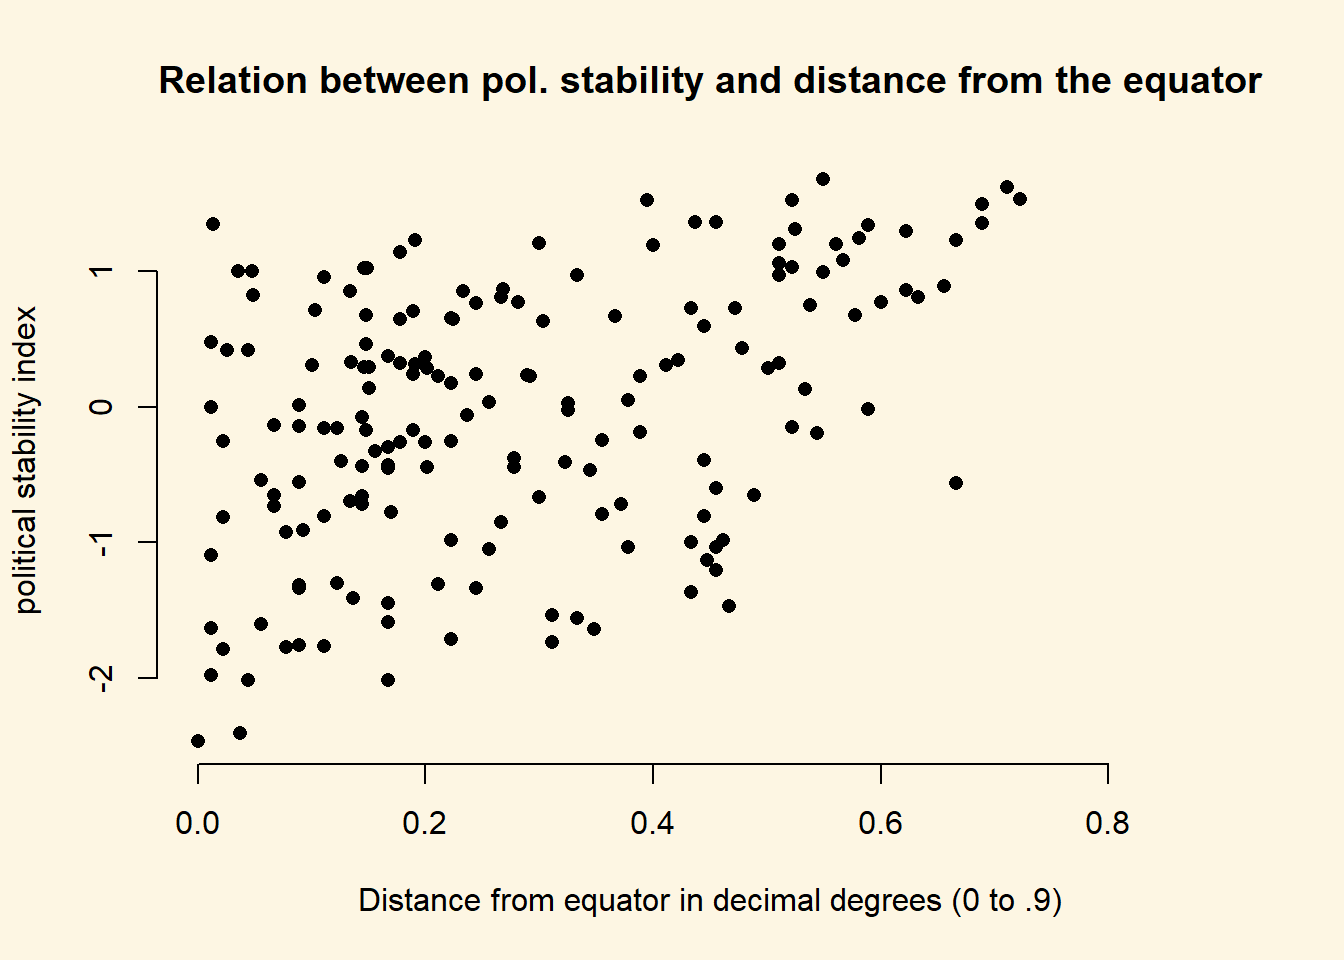
\includegraphics{statistics1_files/figure-latex/unnamed-chunk-225-1.pdf}

\paragraph{Optional Exercise 2}\label{optional-exercise-2}

What is the correlation coefficient of political stability and latitude?

\begin{Shaded}
\begin{Highlighting}[]
\KeywordTok{cor}\NormalTok{(world.data}\OperatorTok{$}\NormalTok{wbgi_pse, world.data}\OperatorTok{$}\NormalTok{lp_lat_abst, }\DataTypeTok{use =} \StringTok{"complete.obs"}\NormalTok{)}
\end{Highlighting}
\end{Shaded}

\begin{verbatim}
[1] 0.4238086
\end{verbatim}

the correlation coefficient ranges from -1 to 1 and is a measure of
linear association of two continuous variables. The variables are
positively related. That means, as we move away from the equator, we
tend to observe higher levels of political stability.

\paragraph{Optional Exercise 3}\label{optional-exercise-3}

If we move away from the equator, how does political stability change?

Political stability tends to increase as we move away from the equator.

\paragraph{Optional Exercise 4}\label{optional-exercise-4}

Does it matter whether we go north or south from the equator?

It does not matter whether we go north or south. Our latitude is
measured in decimal degrees. Thus, a value of 0.9 could correspond to
either the North Pole or the South Pole.

\subsubsection{Advanced Exercises}\label{advanced-exercises-1}

These exercises were hard and go beyond what we expect from you at this
point. Good job, if you were able to solve them!

\paragraph{Advanced Exercise 1}\label{advanced-exercise-1}

Calculate the numerical difference in means (political stability
conditional on colonialization) using the \texttt{means()} function.

Notice: Earlier we dropped missing values on \textbf{undp\_hdi}. We
thereby dropped values that were not missing on \textbf{wbgi\_pse} from
the dataset. That was valuable information. Not reloading the dataset
would be a mistake.

\begin{Shaded}
\begin{Highlighting}[]
\CommentTok{# use full dataset }
\NormalTok{world.data <-}\StringTok{ }\NormalTok{world.data.full}

\KeywordTok{table}\NormalTok{(world.data}\OperatorTok{$}\NormalTok{former_col) }\CommentTok{# check the labels of the former colonies variable }
\end{Highlighting}
\end{Shaded}

\begin{verbatim}

not colonised was colonised 
           72           122 
\end{verbatim}

\begin{Shaded}
\begin{Highlighting}[]
\CommentTok{# mean political stability of not colonised group}
\NormalTok{mean.not.col <-}\StringTok{ }\KeywordTok{mean}\NormalTok{(world.data}\OperatorTok{$}\NormalTok{wbgi_pse[world.data}\OperatorTok{$}\NormalTok{former_col}\OperatorTok{==}\StringTok{"not colonised"}\NormalTok{])}
\NormalTok{mean.not.col}
\end{Highlighting}
\end{Shaded}

\begin{verbatim}
[1] 0.2858409
\end{verbatim}

\begin{Shaded}
\begin{Highlighting}[]
\CommentTok{# mean political stability of colonised group}
\NormalTok{mean.was.col <-}\StringTok{ }\KeywordTok{mean}\NormalTok{(world.data}\OperatorTok{$}\NormalTok{wbgi_pse[world.data}\OperatorTok{$}\NormalTok{former_col}\OperatorTok{==}\StringTok{"was colonised"}\NormalTok{])}
\NormalTok{mean.was.col}
\end{Highlighting}
\end{Shaded}

\begin{verbatim}
[1] -0.231612
\end{verbatim}

\begin{Shaded}
\begin{Highlighting}[]
\CommentTok{# difference in means}
\NormalTok{fd <-}\StringTok{ }\NormalTok{mean.not.col }\OperatorTok{-}\StringTok{ }\NormalTok{mean.was.col}
\NormalTok{fd}
\end{Highlighting}
\end{Shaded}

\begin{verbatim}
[1] 0.5174529
\end{verbatim}

The difference in means is 0.5174529. Countries that were not colonised
are more politically stable.

\paragraph{Advanced Exercise 2}\label{advanced-exercise-2}

Calculate the standard deviation of the difference in means (hint: using
just the \texttt{sd()} function is incorrect in this context).

The standard error of the difference between two means is:

\[ \sqrt{\frac{\sigma^2_{Y_A}}{n_A} + \frac{\sigma^2_{Y_B}}{n_B}} \]

Where \(A\) and \(B\) are the two groups.

\begin{Shaded}
\begin{Highlighting}[]
\CommentTok{# variance of political stability in the two groups}
\NormalTok{var_not_col <-}\StringTok{ }\KeywordTok{var}\NormalTok{(world.data}\OperatorTok{$}\NormalTok{wbgi_pse[world.data}\OperatorTok{$}\NormalTok{former_col}\OperatorTok{==}\StringTok{"not colonised"}\NormalTok{])}
\NormalTok{var_was_col <-}\StringTok{ }\KeywordTok{var}\NormalTok{(world.data}\OperatorTok{$}\NormalTok{wbgi_pse[world.data}\OperatorTok{$}\NormalTok{former_col}\OperatorTok{==}\StringTok{"was colonised"}\NormalTok{])}

\CommentTok{# number of observations in each group}
\NormalTok{n_not_col <-}\StringTok{ }\KeywordTok{length}\NormalTok{(world.data}\OperatorTok{$}\NormalTok{wbgi_pse[world.data}\OperatorTok{$}\NormalTok{former_col}\OperatorTok{==}\StringTok{"not colonised"}\NormalTok{])}
\NormalTok{n_was_col <-}\StringTok{ }\KeywordTok{length}\NormalTok{(world.data}\OperatorTok{$}\NormalTok{wbgi_pse[world.data}\OperatorTok{$}\NormalTok{former_col}\OperatorTok{==}\StringTok{"was colonised"}\NormalTok{])}

\CommentTok{# standard error of the difference in means}
\NormalTok{fd.se <-}\StringTok{ }\KeywordTok{sqrt}\NormalTok{( (var_not_col}\OperatorTok{/}\NormalTok{n_not_col) }\OperatorTok{+}\StringTok{ }\NormalTok{(var_was_col}\OperatorTok{/}\NormalTok{n_was_col)   )}
\NormalTok{fd.se}
\end{Highlighting}
\end{Shaded}

\begin{verbatim}
[1] 0.1492324
\end{verbatim}

The standard error of the difference in means is 0.1492324.

\paragraph{Advanced Exercise 3}\label{advanced-exercise-3}

Is the difference in means more than \(1.96\) standard deviations away
from zero? Interpret the result.

\begin{Shaded}
\begin{Highlighting}[]
\NormalTok{fd }\OperatorTok{-}\StringTok{ }\DecValTok{2}\OperatorTok{*}\NormalTok{fd.se}
\end{Highlighting}
\end{Shaded}

\begin{verbatim}
[1] 0.2189881
\end{verbatim}

The difference in means is further than two standard deviations away
from zero. Given an alpha level of 0.05, we can reject the null
hypothesis that political stability is the same in countries that were
colonised and those that were not.

\paragraph{Advanced Exercise 4}\label{advanced-exercise-4}

We claim, the difference in means in terms of political stability
between countries that were former colonies and those that were not is
0.3. Check this hypothesis.

We use the t-test for the difference in means to test this claim.
Normally, our null would be that the difference in means is zero,
i.e.~there is no difference. Here, the claim is that the difference is
0.3. So, all we have to do is adjust the null hypothesis accordingly.

\begin{Shaded}
\begin{Highlighting}[]
\KeywordTok{t.test}\NormalTok{(world.data}\OperatorTok{$}\NormalTok{wbgi_pse[world.data}\OperatorTok{$}\NormalTok{former_col }\OperatorTok{==}\StringTok{ "not colonised"}\NormalTok{],}
\NormalTok{       world.data}\OperatorTok{$}\NormalTok{wbgi_pse[world.data}\OperatorTok{$}\NormalTok{former_col }\OperatorTok{==}\StringTok{ "was colonised"}\NormalTok{], }
       \DataTypeTok{mu =} \FloatTok{0.3}\NormalTok{, }\DataTypeTok{alt =} \StringTok{"two.sided"}\NormalTok{)}
\end{Highlighting}
\end{Shaded}

\begin{verbatim}

    Welch Two Sample t-test

data:  world.data$wbgi_pse[world.data$former_col == "not colonised"] and world.data$wbgi_pse[world.data$former_col == "was colonised"]
t = 1.4571, df = 139.35, p-value = 0.1473
alternative hypothesis: true difference in means is not equal to 0.3
95 percent confidence interval:
 0.2224004 0.8125053
sample estimates:
 mean of x  mean of y 
 0.2858409 -0.2316120 
\end{verbatim}

We cannot reject the claim that the true difference in means is 0.3.

\paragraph{Advanced Exercise 5}\label{advanced-exercise-5}

First, we drop missings from \textbf{wdi\_gdpc}.

\begin{Shaded}
\begin{Highlighting}[]
\NormalTok{world.data <-}\StringTok{ }\NormalTok{world.data[ }\OperatorTok{!}\KeywordTok{is.na}\NormalTok{(world.data}\OperatorTok{$}\NormalTok{wdi_gdpc), ]}
\end{Highlighting}
\end{Shaded}

An angry citizen who wants to defund the Department of International
Development (DFID) claims that countries that were former colonies have
reached \(75\%\) of the level of wealth of countries that were not
colonised. Check this claim.

The null hypothesis is that there is no difference between the level of
wealth in countries that were former colonies and 0.75 times the level
of wealth in countries that were not former colonies

\begin{Shaded}
\begin{Highlighting}[]
\CommentTok{# the claim of the citizen}
\NormalTok{claim <-}\StringTok{ }\KeywordTok{mean}\NormalTok{(world.data}\OperatorTok{$}\NormalTok{wdi_gdpc[world.data}\OperatorTok{$}\NormalTok{former_col}\OperatorTok{==}\StringTok{"not colonised"}\NormalTok{]) }\OperatorTok{*}\StringTok{ }\FloatTok{0.75} 
\NormalTok{claim}
\end{Highlighting}
\end{Shaded}

\begin{verbatim}
[1] 12311.54
\end{verbatim}

\begin{Shaded}
\begin{Highlighting}[]
\CommentTok{# estimated level of wealth in countries that were colonised}
\NormalTok{estimate <-}\StringTok{ }\KeywordTok{mean}\NormalTok{(world.data}\OperatorTok{$}\NormalTok{wdi_gdpc[world.data}\OperatorTok{$}\NormalTok{former_col}\OperatorTok{==}\StringTok{"was colonised"}\NormalTok{])}
\NormalTok{estimate}
\end{Highlighting}
\end{Shaded}

\begin{verbatim}
[1] 6599.714
\end{verbatim}

Our estimate is roughly half the angry citizen's claim. The substantial
difference is huge. To cover all our bases, let's perform the t-test for
the difference in means.

How would we do this though? This one is tricky because the citizen's
claim is not actually in our data. At the same time we don't know the
true level of wealth in countries that were not colonised, we only have
an estimate. We have to manipulate our data to get there.

First, we create a copy of the wealth variable with a new name.

\begin{Shaded}
\begin{Highlighting}[]
\NormalTok{world.data}\OperatorTok{$}\NormalTok{angry_gdp <-}\StringTok{ }\NormalTok{world.data}\OperatorTok{$}\NormalTok{wdi_gdpc}
\end{Highlighting}
\end{Shaded}

Now, we adjust the level of wealth in the group of countries that were
not colonised down to the citizen's claim. The citizen's claim is that
we should then not find a difference in means between the two groups
(``was colonised'' and ``not colonised'') anymore.

\begin{Shaded}
\begin{Highlighting}[]
\NormalTok{world.data}\OperatorTok{$}\NormalTok{angry_gdp[world.data}\OperatorTok{$}\NormalTok{former_col}\OperatorTok{==}\StringTok{"not colonised"}\NormalTok{] <-}\StringTok{ }\NormalTok{world.data}\OperatorTok{$}\NormalTok{angry_gdp[world.data}\OperatorTok{$}\NormalTok{former_col}\OperatorTok{==}\StringTok{"not colonised"}\NormalTok{] }\OperatorTok{*}\StringTok{ }\FloatTok{0.75}
\KeywordTok{mean}\NormalTok{(world.data}\OperatorTok{$}\NormalTok{angry_gdp[world.data}\OperatorTok{$}\NormalTok{former_col}\OperatorTok{==}\StringTok{"not colonised"}\NormalTok{])}
\end{Highlighting}
\end{Shaded}

\begin{verbatim}
[1] 12311.54
\end{verbatim}

We can see that the level of mean wealth of our manipulated variable for
countries that were not colonised now corresponds to the citizen's
claim. We can now check the difference in means.

\begin{Shaded}
\begin{Highlighting}[]
\KeywordTok{t.test}\NormalTok{(world.data}\OperatorTok{$}\NormalTok{angry_gdp[world.data}\OperatorTok{$}\NormalTok{former_col}\OperatorTok{==}\StringTok{"not colonised"}\NormalTok{],}
\NormalTok{       world.data}\OperatorTok{$}\NormalTok{angry_gdp[world.data}\OperatorTok{$}\NormalTok{former_col}\OperatorTok{==}\StringTok{"was colonised"}\NormalTok{], }
       \DataTypeTok{mu =} \DecValTok{0}\NormalTok{, }\DataTypeTok{alt =} \StringTok{"two.sided"}\NormalTok{)}
\end{Highlighting}
\end{Shaded}

\begin{verbatim}

    Welch Two Sample t-test

data:  world.data$angry_gdp[world.data$former_col == "not colonised"] and world.data$angry_gdp[world.data$former_col == "was colonised"]
t = 3.6218, df = 127.72, p-value = 0.0004206
alternative hypothesis: true difference in means is not equal to 0
95 percent confidence interval:
 2591.29 8832.37
sample estimates:
mean of x mean of y 
12311.544  6599.714 
\end{verbatim}

Clearly, we can reject the citizen's claim. Our p value implies that the
probability that we see this huge difference in our data, given that
there really is no difference, is \(0.04\%\). Our conventional alpha
level is \(5\%\).

\section{Revision: Sample Variance and Sample Standard Deviation;
Hypothesis testing and Confidence
Intervals}\label{revision-sample-variance-and-sample-standard-deviation-hypothesis-testing-and-confidence-intervals}

In this seminar, we revise the concepts of the standard deviation, the
sampling variance, hypothesis testing and confidence intervals. We will
also learn some more data manipulation and working with the random
number generator.

\subsection{Seminar}\label{seminar-4}

Let's remove all objects from our workspace and set the working
directory.

\begin{Shaded}
\begin{Highlighting}[]
\KeywordTok{rm}\NormalTok{(}\DataTypeTok{list=}\KeywordTok{ls}\NormalTok{())}
\KeywordTok{setwd}\NormalTok{(}\StringTok{"~/statistics1"}\NormalTok{)}
\end{Highlighting}
\end{Shaded}

\subsubsection{Sample Variance and Sample Standard
Deviation}\label{sample-variance-and-sample-standard-deviation}

The sample variance and sample standard deviation inform us about the
degree of variability of our data. Suppose, we were to roll the dice 5
times. We could then compute the mean value that we roll. The sample
standard deviation measures by how much an average roll of the dice will
deviate from the mean value.

We start rolling the dice, using R's random number generator and the
\texttt{runif()} function. The function randomly draws numbers from a
uniform distribution. In a uniform distribution each value has the same
probability of being drawn. All six sides of a die should be equally
likely if the die is fair. Hence, the uniform distribution.

\texttt{runif()} takes three arguments. \texttt{n} is the number of
values to be drawn. \texttt{min} is the minimum value and \texttt{max}
is the maximum value.

\begin{Shaded}
\begin{Highlighting}[]
\CommentTok{# random draw of 10 values from a uniform distribution}
\NormalTok{dice <-}\StringTok{ }\KeywordTok{runif}\NormalTok{(}\DataTypeTok{n =} \DecValTok{10}\NormalTok{, }\DataTypeTok{min =} \DecValTok{1}\NormalTok{, }\DataTypeTok{max =} \DecValTok{7}\NormalTok{)}
\NormalTok{dice}
\end{Highlighting}
\end{Shaded}

\begin{verbatim}
 [1] 5.843582 3.542866 5.548386 5.917123 3.851856 2.040016 3.087642
 [8] 1.213291 5.969721 3.809420
\end{verbatim}

We have indeed drawn 10 numbers but they are not integers as we would
like---we want to simulate a die, so the values should be 1, 2, 3, 4, 5
or 6. We will return to this in a moment but for now let's return to the
randomness. Let's draw 10 numbers again:

\begin{Shaded}
\begin{Highlighting}[]
\CommentTok{# random draw of 10 values from a uniform distribution}
\NormalTok{dice2 <-}\StringTok{ }\KeywordTok{runif}\NormalTok{(}\DataTypeTok{n =} \DecValTok{10}\NormalTok{, }\DataTypeTok{min =} \DecValTok{1}\NormalTok{, }\DataTypeTok{max =} \DecValTok{7}\NormalTok{)}

\CommentTok{# first draw}
\NormalTok{dice}
\end{Highlighting}
\end{Shaded}

\begin{verbatim}
 [1] 5.843582 3.542866 5.548386 5.917123 3.851856 2.040016 3.087642
 [8] 1.213291 5.969721 3.809420
\end{verbatim}

\begin{Shaded}
\begin{Highlighting}[]
\CommentTok{# second draw}
\NormalTok{dice2}
\end{Highlighting}
\end{Shaded}

\begin{verbatim}
 [1] 6.774116 6.071745 6.151463 4.765166 1.250423 4.681061 6.340679
 [8] 3.205550 4.108115 4.061521
\end{verbatim}

The numbers of the first and second roll differ because we have drawn
values at random. To make our results replicate and to ensure that
everyone in the seminar works with the same numbers, we set R's random
number generator with the \texttt{set.seed()} function. As argument we
plug in some arbitrary value (it does not matter which but using a
different one will lead to a different quasi-random draw).

\begin{Shaded}
\begin{Highlighting}[]
\CommentTok{# set random number generator}
\KeywordTok{set.seed}\NormalTok{(}\DecValTok{123}\NormalTok{)}

\CommentTok{# random draw of 10 values from a uniform distribution}
\NormalTok{dice <-}\StringTok{ }\KeywordTok{runif}\NormalTok{(}\DataTypeTok{n =} \DecValTok{10}\NormalTok{, }\DataTypeTok{min =} \DecValTok{1}\NormalTok{, }\DataTypeTok{max =} \DecValTok{7}\NormalTok{)}
\NormalTok{dice}
\end{Highlighting}
\end{Shaded}

\begin{verbatim}
 [1] 2.725465 5.729831 3.453862 6.298104 6.642804 1.273339 4.168633
 [8] 6.354514 4.308610 3.739688
\end{verbatim}

You should all have the same values. If not, run \texttt{set.seed()}
again and then do the random draw once. If you do it more than once, the
numbers will change. Let's see how this works:

\begin{Shaded}
\begin{Highlighting}[]
\CommentTok{# set random number generator}
\KeywordTok{set.seed}\NormalTok{(}\DecValTok{123}\NormalTok{)}

\CommentTok{# 1st random draw of 10 values from a uniform distribution}
\NormalTok{dice <-}\StringTok{ }\KeywordTok{runif}\NormalTok{(}\DataTypeTok{n =} \DecValTok{10}\NormalTok{, }\DataTypeTok{min =} \DecValTok{1}\NormalTok{, }\DataTypeTok{max =} \DecValTok{7}\NormalTok{)}
\NormalTok{dice}
\end{Highlighting}
\end{Shaded}

\begin{verbatim}
 [1] 2.725465 5.729831 3.453862 6.298104 6.642804 1.273339 4.168633
 [8] 6.354514 4.308610 3.739688
\end{verbatim}

\begin{Shaded}
\begin{Highlighting}[]
\CommentTok{# 2nd random draw of 10 values from a uniform distribution}
\NormalTok{dice2 <-}\StringTok{ }\KeywordTok{runif}\NormalTok{(}\DataTypeTok{n =} \DecValTok{10}\NormalTok{, }\DataTypeTok{min =} \DecValTok{1}\NormalTok{, }\DataTypeTok{max =} \DecValTok{7}\NormalTok{)}
\NormalTok{dice2}
\end{Highlighting}
\end{Shaded}

\begin{verbatim}
 [1] 6.741000 3.720005 5.065424 4.435800 1.617548 6.398950 2.476526
 [8] 1.252357 2.967524 6.727022
\end{verbatim}

\begin{Shaded}
\begin{Highlighting}[]
\CommentTok{# reset random number generator}
\KeywordTok{set.seed}\NormalTok{(}\DecValTok{123}\NormalTok{)}

\CommentTok{# 3rd random draw of 10 values from a uniform distribution}
\NormalTok{dice3 <-}\StringTok{ }\KeywordTok{runif}\NormalTok{(}\DataTypeTok{n =} \DecValTok{10}\NormalTok{, }\DataTypeTok{min =} \DecValTok{1}\NormalTok{, }\DataTypeTok{max =} \DecValTok{7}\NormalTok{)}
\NormalTok{dice3}
\end{Highlighting}
\end{Shaded}

\begin{verbatim}
 [1] 2.725465 5.729831 3.453862 6.298104 6.642804 1.273339 4.168633
 [8] 6.354514 4.308610 3.739688
\end{verbatim}

\begin{Shaded}
\begin{Highlighting}[]
\CommentTok{# 4th random draw of 10 values from a uniform distribution}
\NormalTok{dice4 <-}\StringTok{ }\KeywordTok{runif}\NormalTok{(}\DataTypeTok{n =} \DecValTok{10}\NormalTok{, }\DataTypeTok{min =} \DecValTok{1}\NormalTok{, }\DataTypeTok{max =} \DecValTok{7}\NormalTok{)}
\NormalTok{dice4}
\end{Highlighting}
\end{Shaded}

\begin{verbatim}
 [1] 6.741000 3.720005 5.065424 4.435800 1.617548 6.398950 2.476526
 [8] 1.252357 2.967524 6.727022
\end{verbatim}

As you can see, the the draws from \textbf{dice} and \textbf{dice3} are
the same and the draws from \textbf{dice2} and \textbf{dice4} are the
same as well. Let's make the values integers with the
\texttt{as.integer()} function which simply cuts off all decimal places.

\begin{Shaded}
\begin{Highlighting}[]
\CommentTok{# reset random number generator}
\KeywordTok{set.seed}\NormalTok{(}\DecValTok{123}\NormalTok{)}
\CommentTok{# random draw of 10 numbers from a uniform distribution with minimum 1 and maximum 7}
\NormalTok{dice <-}\StringTok{ }\KeywordTok{runif}\NormalTok{(}\DecValTok{10}\NormalTok{, }\DecValTok{1}\NormalTok{, }\DecValTok{7}\NormalTok{)}
\CommentTok{# cut off decimals places}
\NormalTok{dice <-}\StringTok{ }\KeywordTok{as.integer}\NormalTok{(dice)}
\NormalTok{dice}
\end{Highlighting}
\end{Shaded}

\begin{verbatim}
 [1] 2 5 3 6 6 1 4 6 4 3
\end{verbatim}

\begin{Shaded}
\begin{Highlighting}[]
\CommentTok{# frequency of dice rolls}
\KeywordTok{table}\NormalTok{(dice)}
\end{Highlighting}
\end{Shaded}

\begin{verbatim}
dice
1 2 3 4 5 6 
1 1 2 2 1 3 
\end{verbatim}

We have rolled a six relatively often. All sides should be equally
likely but due to sampling variability, we have rolled the six most
often. The expected value of a die is 3.5. That is:
\[ 1 \times \frac{1}{6} + 2 \times \frac{1}{6} + 3 \times \frac{1}{6} + 4 \times \frac{1}{6} + 5 \times \frac{1}{6} + 6 \times \frac{1}{6} = 3.5\]

We compute the mean in our sample and the standard deviation. Let's
start with the mean. Do so yourself but do not use the in-built
function.

\begin{Shaded}
\begin{Highlighting}[]
\NormalTok{dice.sum <-}\StringTok{ }\NormalTok{dice[}\DecValTok{1}\NormalTok{] }\OperatorTok{+}\StringTok{ }\NormalTok{dice[}\DecValTok{2}\NormalTok{] }\OperatorTok{+}\StringTok{ }\NormalTok{dice[}\DecValTok{3}\NormalTok{] }\OperatorTok{+}\StringTok{ }\NormalTok{dice[}\DecValTok{4}\NormalTok{] }\OperatorTok{+}\StringTok{ }\NormalTok{dice[}\DecValTok{5}\NormalTok{] }\OperatorTok{+}\StringTok{ }\NormalTok{dice[}\DecValTok{6}\NormalTok{] }\OperatorTok{+}\StringTok{ }\NormalTok{dice[}\DecValTok{7}\NormalTok{] }\OperatorTok{+}\StringTok{ }\NormalTok{dice[}\DecValTok{8}\NormalTok{] }\OperatorTok{+}\StringTok{ }\NormalTok{dice[}\DecValTok{9}\NormalTok{] }\OperatorTok{+}\StringTok{ }\NormalTok{dice[}\DecValTok{10}\NormalTok{]}
\NormalTok{dice.mean <-}\StringTok{ }\NormalTok{dice.sum }\OperatorTok{/}\StringTok{ }\DecValTok{10}  
\NormalTok{dice.mean}
\end{Highlighting}
\end{Shaded}

\begin{verbatim}
[1] 4
\end{verbatim}

We would have gotten the same result from the \texttt{mean()} function.

The sample standard deviation tells by how much an average roll of the
dice differs from the estimated sample mean. Estimate the sample
standard deviation on your own without using the \texttt{sd()} function.
Do not copy. Type everything yourself.

\begin{Shaded}
\begin{Highlighting}[]
\NormalTok{numerator <-}\StringTok{ }\NormalTok{( (dice[}\DecValTok{1}\NormalTok{] }\OperatorTok{-}\StringTok{ }\NormalTok{dice.mean)}\OperatorTok{^}\DecValTok{2} \OperatorTok{+}\StringTok{ }\NormalTok{(dice[}\DecValTok{2}\NormalTok{] }\OperatorTok{-}\StringTok{ }\NormalTok{dice.mean)}\OperatorTok{^}\DecValTok{2} \OperatorTok{+}\StringTok{ }\NormalTok{(dice[}\DecValTok{3}\NormalTok{] }\OperatorTok{-}\StringTok{ }\NormalTok{dice.mean)}\OperatorTok{^}\DecValTok{2}  \OperatorTok{+}
\StringTok{                 }\NormalTok{(dice[}\DecValTok{4}\NormalTok{] }\OperatorTok{-}\StringTok{ }\NormalTok{dice.mean)}\OperatorTok{^}\DecValTok{2} \OperatorTok{+}\StringTok{ }\NormalTok{(dice[}\DecValTok{5}\NormalTok{] }\OperatorTok{-}\StringTok{ }\NormalTok{dice.mean)}\OperatorTok{^}\DecValTok{2} \OperatorTok{+}\StringTok{ }\NormalTok{(dice[}\DecValTok{6}\NormalTok{] }\OperatorTok{-}\StringTok{ }\NormalTok{dice.mean)}\OperatorTok{^}\DecValTok{2} \OperatorTok{+}
\StringTok{                 }\NormalTok{(dice[}\DecValTok{7}\NormalTok{] }\OperatorTok{-}\StringTok{ }\NormalTok{dice.mean)}\OperatorTok{^}\DecValTok{2} \OperatorTok{+}\StringTok{ }\NormalTok{(dice[}\DecValTok{8}\NormalTok{] }\OperatorTok{-}\StringTok{ }\NormalTok{dice.mean)}\OperatorTok{^}\DecValTok{2} \OperatorTok{+}\StringTok{ }\NormalTok{(dice[}\DecValTok{9}\NormalTok{] }\OperatorTok{-}\StringTok{ }\NormalTok{dice.mean)}\OperatorTok{^}\DecValTok{2} \OperatorTok{+}
\StringTok{                 }\NormalTok{(dice[}\DecValTok{10}\NormalTok{] }\OperatorTok{-}\StringTok{ }\NormalTok{dice.mean)}\OperatorTok{^}\DecValTok{2}\NormalTok{ )}
\NormalTok{std.dev <-}\StringTok{ }\KeywordTok{sqrt}\NormalTok{( (numerator }\OperatorTok{/}\StringTok{ }\DecValTok{9}\NormalTok{) )}
\NormalTok{std.dev}
\end{Highlighting}
\end{Shaded}

\begin{verbatim}
[1] 1.763834
\end{verbatim}

An average deviation from the sample mean is 1.76.

\subsubsection{T test for the sample
mean}\label{t-test-for-the-sample-mean}

Our estimate of the mean is 4. The expected value is 3.5. Is this
evidence that the die is loaded? The null hypothesis is that the die is
fair. The alternative hypothesis is that the die is loaded.

Answer this question on your own by computing and interpreting the t
value.

\begin{Shaded}
\begin{Highlighting}[]
\CommentTok{# standard error of the sample mean}
\NormalTok{std.err <-}\StringTok{ }\NormalTok{std.dev }\OperatorTok{/}\StringTok{ }\KeywordTok{sqrt}\NormalTok{(}\DecValTok{10}\NormalTok{)}

\CommentTok{# t value}
\NormalTok{t.value <-}\StringTok{ }\NormalTok{(}\DecValTok{4} \OperatorTok{-}\StringTok{ }\FloatTok{3.5}\NormalTok{) }\OperatorTok{/}\StringTok{ }\NormalTok{std.err}
\NormalTok{t.value  }
\end{Highlighting}
\end{Shaded}

\begin{verbatim}
[1] 0.8964215
\end{verbatim}

Clearly, we cannot reject the null hypothesis. The estimated difference
between our sample mean and the population mean is 0.5. This value is
0.9 standard errors away from the population mean under the null
hypothesis (3.5). We do not know the critical value for the t
distribution here because we are in a small sample. However, it must be
bigger than 1.96. Our t value is clearly smaller, therefore, we
\textbf{\emph{cannot}} reject the null hypothesis. That is not
surprising, given that we have drawn from a uniform distribution, i.e.,
our sampling process was fair by definition.

Let's back up. The standard error quantifies the average difference
between mean estimates that are due to sampling variability (chance).
Put differently, the standard error approximates the average difference
between the population mean and our sample estimate.

Now. Compute the variance of the mean on your own. Try yourself before
you check the code.

\begin{Shaded}
\begin{Highlighting}[]
\CommentTok{# sample variance}
\NormalTok{variance <-}\StringTok{ }\NormalTok{numerator }\OperatorTok{/}\StringTok{ }\DecValTok{9}

\CommentTok{# variance of the mean}
\NormalTok{var.mean <-}\StringTok{ }\NormalTok{variance }\OperatorTok{/}\StringTok{ }\DecValTok{10}
\NormalTok{var.mean}
\end{Highlighting}
\end{Shaded}

\begin{verbatim}
[1] 0.3111111
\end{verbatim}

The correct answer is 0.31. Now, compute the standard error of the mean
from your variance of the mean. Try yourself.

\[ s^2_{\bar{X}} = \frac{s_{x}^2}{n} = (\sqrt{ \frac{s_{x}}{\sqrt{n}}})^2 \]

\begin{Shaded}
\begin{Highlighting}[]
\CommentTok{# variance of the mean}
\KeywordTok{sqrt}\NormalTok{(var.mean)}
\end{Highlighting}
\end{Shaded}

\begin{verbatim}
[1] 0.5577734
\end{verbatim}

Let's estimate the p value from a t distribution with the correct amount
of degrees of freedom.

\begin{Shaded}
\begin{Highlighting}[]
\NormalTok{p.value <-}\StringTok{ }\NormalTok{(}\DecValTok{1} \OperatorTok{-}\StringTok{ }\KeywordTok{pt}\NormalTok{(t.value, }\DataTypeTok{df =} \DecValTok{9}\NormalTok{))}\OperatorTok{*}\DecValTok{2}
\NormalTok{p.value}
\end{Highlighting}
\end{Shaded}

\begin{verbatim}
[1] 0.3933733
\end{verbatim}

The probability that we roll a fair die 10 times and get a sample mean
of 4 is 39 percent. That is not unlikely at all. We are far from
rejecting the null hypothesis.

We now construct the confidence interval around our mean estimate. To
re-cap, we construct the confidence interval as:

\[ \bar{Y} \pm \mathrm{critical \: value} \times  SE(\bar{Y})  \]

First, we need the critical value (for an alpha level of 0.05). We get
the critical value from the quantile function of the t distribution with
\(n-1\) degrees of freedom.

\begin{Shaded}
\begin{Highlighting}[]
\KeywordTok{qt}\NormalTok{(}\DataTypeTok{p =} \FloatTok{0.975}\NormalTok{, }\DataTypeTok{df =} \DecValTok{9}\NormalTok{)}
\end{Highlighting}
\end{Shaded}

\begin{verbatim}
[1] 2.262157
\end{verbatim}

where \texttt{p} is the cumulative probability and \texttt{df} is the
degrees of freedom. The critical value in a t distribution with 9
degrees of freedom is 2.262157.

Construct the lower and upper bounds of the confidence interval
yourself.

\begin{Shaded}
\begin{Highlighting}[]
\CommentTok{# lower bound}
\NormalTok{lb <-}\StringTok{ }\NormalTok{dice.mean }\OperatorTok{-}\StringTok{ }\KeywordTok{qt}\NormalTok{(}\DataTypeTok{p =} \FloatTok{0.975}\NormalTok{, }\DataTypeTok{df =} \DecValTok{9}\NormalTok{) }\OperatorTok{*}\StringTok{ }\NormalTok{std.err}
\CommentTok{# upper bound}
\NormalTok{ub <-}\StringTok{ }\NormalTok{dice.mean }\OperatorTok{+}\StringTok{ }\KeywordTok{qt}\NormalTok{(}\DataTypeTok{p =} \FloatTok{0.975}\NormalTok{, }\DataTypeTok{df =} \DecValTok{9}\NormalTok{) }\OperatorTok{*}\StringTok{ }\NormalTok{std.err}

\CommentTok{# confidence interval}
\NormalTok{lb}
\end{Highlighting}
\end{Shaded}

\begin{verbatim}
[1] 2.738229
\end{verbatim}

\begin{Shaded}
\begin{Highlighting}[]
\NormalTok{ub}
\end{Highlighting}
\end{Shaded}

\begin{verbatim}
[1] 5.261771
\end{verbatim}

With 95 percent probability (where the probability is the long-run
relative frequency), the population mean is within the confidence
interval.

Clearly, the population mean under the assumption that the null
hypothesis is true (3.5), is within this interval.

Run a t test using the \texttt{t.test()} function yourself.

\begin{Shaded}
\begin{Highlighting}[]
\KeywordTok{t.test}\NormalTok{(dice,}
       \DataTypeTok{mu =} \FloatTok{3.5}\NormalTok{,}
       \DataTypeTok{conf.level =}\NormalTok{ .}\DecValTok{95}\NormalTok{)}
\end{Highlighting}
\end{Shaded}

\begin{verbatim}

    One Sample t-test

data:  dice
t = 0.89642, df = 9, p-value = 0.3934
alternative hypothesis: true mean is not equal to 3.5
95 percent confidence interval:
 2.738229 5.261771
sample estimates:
mean of x 
        4 
\end{verbatim}

The \texttt{t.test()} function is more convenient than estimating
everything by hand. The results are the same.

\subsubsection{T test for the difference in
means}\label{t-test-for-the-difference-in-means}

We will now test the difference between two dice. First, remove
everything from the workspace on your own.

\begin{Shaded}
\begin{Highlighting}[]
\CommentTok{# remove everything from the workspace}
\KeywordTok{rm}\NormalTok{(}\DataTypeTok{list =} \KeywordTok{ls}\NormalTok{())}
\end{Highlighting}
\end{Shaded}

Set the random number generator to 1234.

\begin{Shaded}
\begin{Highlighting}[]
\KeywordTok{set.seed}\NormalTok{(}\DecValTok{1234}\NormalTok{)}
\end{Highlighting}
\end{Shaded}

Generate a vector of 100 rolls of a fair dice on your own and show the
results in a frequency table.

\begin{Shaded}
\begin{Highlighting}[]
\NormalTok{fair.die <-}\StringTok{ }\KeywordTok{runif}\NormalTok{(}\DataTypeTok{n =} \DecValTok{100}\NormalTok{, }\DataTypeTok{min =} \DecValTok{1}\NormalTok{, }\DataTypeTok{max =} \DecValTok{7}\NormalTok{)}
\NormalTok{fair.die <-}\StringTok{ }\KeywordTok{as.integer}\NormalTok{(fair.die)}
\KeywordTok{table}\NormalTok{(fair.die)}
\end{Highlighting}
\end{Shaded}

\begin{verbatim}
fair.die
 1  2  3  4  5  6 
21 28  6 20 13 12 
\end{verbatim}

The absolute number are not that great to see the distribution of values
at a glance. Create a table that shows the proportions of each outcome.

\begin{Shaded}
\begin{Highlighting}[]
\KeywordTok{table}\NormalTok{(fair.die) }\OperatorTok{/}\StringTok{ }\KeywordTok{sum}\NormalTok{(}\KeywordTok{table}\NormalTok{(fair.die))}
\end{Highlighting}
\end{Shaded}

\begin{verbatim}
fair.die
   1    2    3    4    5    6 
0.21 0.28 0.06 0.20 0.13 0.12 
\end{verbatim}

Calculate the mean.

\begin{Shaded}
\begin{Highlighting}[]
\KeywordTok{mean}\NormalTok{(fair.die)}
\end{Highlighting}
\end{Shaded}

\begin{verbatim}
[1] 3.12
\end{verbatim}

Although, the proportions look like we rolled the lower numbers way too
often, we are not too far away from the population mean (3.5).

Now, we create a loaded die. We draw randomly from a normal distribution
with mean 4.5 and standard deviation 1.5.

\begin{Shaded}
\begin{Highlighting}[]
\NormalTok{loaded.die <-}\StringTok{ }\KeywordTok{rnorm}\NormalTok{(}\DataTypeTok{n =} \DecValTok{100}\NormalTok{, }\DataTypeTok{mean =} \FloatTok{4.5}\NormalTok{, }\DataTypeTok{sd =} \FloatTok{1.5}\NormalTok{)}
\NormalTok{loaded.die <-}\StringTok{ }\KeywordTok{as.integer}\NormalTok{(loaded.die)}
\KeywordTok{table}\NormalTok{(loaded.die)}
\end{Highlighting}
\end{Shaded}

\begin{verbatim}
loaded.die
 1  2  3  4  5  6  7  8 
 2 13 19 28 23  8  6  1 
\end{verbatim}

Oops, we rolled 6 seven's and 1 eight. Let's change these to sixes. We
use the square brackets to index the elements of the \textbf{loaded.die}
vector. We use the \texttt{which()} function to identify the elements
that are greater than 6. Finally, we change these values to 6.

\begin{Shaded}
\begin{Highlighting}[]
\NormalTok{loaded.die[ }\KeywordTok{which}\NormalTok{(loaded.die }\OperatorTok{>}\StringTok{ }\DecValTok{6}\NormalTok{) ] <-}\StringTok{ }\DecValTok{6}
\KeywordTok{table}\NormalTok{(loaded.die)}
\end{Highlighting}
\end{Shaded}

\begin{verbatim}
loaded.die
 1  2  3  4  5  6 
 2 13 19 28 23 15 
\end{verbatim}

Now, estimate the 2 means (of the fair die and the loaded die) yourself.
Next, estimate the difference in means. You may use the \texttt{mean()}
function.

\begin{Shaded}
\begin{Highlighting}[]
\CommentTok{# mean in the 2 groups}
\KeywordTok{mean}\NormalTok{(fair.die)}
\end{Highlighting}
\end{Shaded}

\begin{verbatim}
[1] 3.12
\end{verbatim}

\begin{Shaded}
\begin{Highlighting}[]
\KeywordTok{mean}\NormalTok{(loaded.die)}
\end{Highlighting}
\end{Shaded}

\begin{verbatim}
[1] 4.02
\end{verbatim}

\begin{Shaded}
\begin{Highlighting}[]
\CommentTok{# first difference (difference in means)}
\NormalTok{fd <-}\StringTok{ }\KeywordTok{mean}\NormalTok{(fair.die) }\OperatorTok{-}\StringTok{ }\KeywordTok{mean}\NormalTok{(loaded.die)}
\NormalTok{fd}
\end{Highlighting}
\end{Shaded}

\begin{verbatim}
[1] -0.9
\end{verbatim}

The difference suggests that we roll larger values with the loaded die.
Is the difference statistically detectable? To find out, we carry out
the t test for the difference in means. Our dependent interval scaled
variable is the value of the roll of the dice. The our independent
binary variable is whether the die is loaded or not.

Compute the standard error for the difference in means on your own.

\[ SE(Y_{X=0} - Y_{X=1}) = \sqrt{ \frac{s_{Y_{X=0}}^2}{n_{X=0}} + \frac{s_{Y_{X=1}}^2}{n_{X=1}}}  \]

where \(s_{Y_{X=0}}^2\) is the variance in the first group and
\(s_{Y_{X=1}}^2\) is the variance in the second group. The number of
observations in the first group is \(n_{X=0}\) and the number of
observations in the second group is \(n_{X=1}\).

The result is 0.2161462. Try until you get it. You may use the
\texttt{var()} function.

\begin{Shaded}
\begin{Highlighting}[]
\CommentTok{# standard error of the first difference}
\NormalTok{se.fd <-}\StringTok{ }\KeywordTok{sqrt}\NormalTok{( ((}\KeywordTok{var}\NormalTok{(fair.die) }\OperatorTok{/}\StringTok{ }\DecValTok{100}\NormalTok{) }\OperatorTok{+}\StringTok{ }\NormalTok{(}\KeywordTok{var}\NormalTok{(loaded.die) }\OperatorTok{/}\StringTok{ }\DecValTok{100}\NormalTok{)) )}
\NormalTok{se.fd}
\end{Highlighting}
\end{Shaded}

\begin{verbatim}
[1] 0.2161462
\end{verbatim}

Now, that we have the standard error of the difference in means, compute
the t statistic on your own (without using the \texttt{t.test()}
function).

\begin{Shaded}
\begin{Highlighting}[]
\CommentTok{# standard error of the first difference}
\NormalTok{t.value <-}\StringTok{ }\NormalTok{(}\KeywordTok{mean}\NormalTok{(fair.die) }\OperatorTok{-}\StringTok{ }\KeywordTok{mean}\NormalTok{(loaded.die)) }\OperatorTok{/}\StringTok{ }\NormalTok{se.fd}
\NormalTok{t.value}
\end{Highlighting}
\end{Shaded}

\begin{verbatim}
[1] -4.163848
\end{verbatim}

The t value is large and our sample size is also large. We can take the
critical from a normal distribution. For an alpha level of 0.05, the
critical value is \(1.96\).

Construct the confidence interval for the difference in means yourself.

\begin{Shaded}
\begin{Highlighting}[]
\CommentTok{# lower bound}
\NormalTok{lb <-}\StringTok{ }\NormalTok{fd }\OperatorTok{-}\StringTok{ }\FloatTok{1.96} \OperatorTok{*}\StringTok{ }\NormalTok{se.fd}
\CommentTok{# upper bound}
\NormalTok{ub <-}\StringTok{ }\NormalTok{fd }\OperatorTok{+}\StringTok{ }\FloatTok{1.96} \OperatorTok{*}\StringTok{ }\NormalTok{se.fd}

\NormalTok{lb}
\end{Highlighting}
\end{Shaded}

\begin{verbatim}
[1] -1.323647
\end{verbatim}

\begin{Shaded}
\begin{Highlighting}[]
\NormalTok{ub}
\end{Highlighting}
\end{Shaded}

\begin{verbatim}
[1] -0.4763534
\end{verbatim}

The confidence interval for the difference in means ranges from -1.32 to
-0.48. Clearly, the difference in means is smaller than 0. We can reject
the null hypothesis that there is no difference between the loaded die
and the fair die because 0 is not within the confidence interval.

Let's estimate the p value: i.e., the probability that we estimate a
difference in means of -0.9 given that there really is no difference
between the fair die and the loaded die.

The result is 3.129287e-05. Try until you get it. You can use the
\texttt{pnrom()} function to get the cumulative probability from a
standard normal distribution.

\begin{Shaded}
\begin{Highlighting}[]
\CommentTok{# 1st way}
\KeywordTok{pnorm}\NormalTok{( t.value ) }\OperatorTok{*}\StringTok{ }\DecValTok{2}
\end{Highlighting}
\end{Shaded}

\begin{verbatim}
[1] 0.00003129287
\end{verbatim}

\begin{Shaded}
\begin{Highlighting}[]
\CommentTok{# 2nd way}
\NormalTok{(}\DecValTok{1} \OperatorTok{-}\StringTok{ }\KeywordTok{pnorm}\NormalTok{( }\KeywordTok{abs}\NormalTok{(t.value) )) }\OperatorTok{*}\DecValTok{2} 
\end{Highlighting}
\end{Shaded}

\begin{verbatim}
[1] 0.00003129287
\end{verbatim}

We can reject the null hypothesis. The loaded die is different from the
fair die.

\subsubsection{Exercises}\label{exercises-4}

\begin{enumerate}
\def\labelenumi{\arabic{enumi}.}
\tightlist
\item
  Create a vector of a fair die and a vector of a loaded die with (25)
  observations such that you cannot distinguish the dice with a
  difference in means test. Carry out the t-test.
\item
  Re-create the dice but increase the number of observations to 1000.
  Does the result of the t test change?
\item
  \href{https://www.cambridge.org/core/journals/journal-of-economic-history/article/ordinary-economic-voting-behavior-in-the-extraordinary-election-of-adolf-hitler/8C79A0AB9DA174B7D81A6EB313B1EDFC}{Ordinary
  Economic Voting Behavior in the Extraordinary Election of Adolf
  Hitler} Download and then load
  \texttt{who\_voted\_nazi\_in\_1932.csv}. who voted nazi in 1932 data
  Codebook: 
\end{enumerate}

\begin{longtable}[]{@{}ll@{}}
\toprule
Variable & Description\tabularnewline
\midrule
\endhead
sharenazis & Percent of the vote Nazis received in the
district\tabularnewline
nazivote & Number of Nazi votes\tabularnewline
nvoter & Total number of eligible voters\tabularnewline
shareblue & Percent of blue-collar potential voters\tabularnewline
sharewhite & Percent of white-collar potential voters\tabularnewline
shareself & Percent of self-employed potential voters\tabularnewline
sharedomestic & Percent of domestically employed potential
voters\tabularnewline
shareunemployed & Percent of unemployed potential voters\tabularnewline
\bottomrule
\end{longtable}

\begin{enumerate}
\def\labelenumi{\arabic{enumi}.}
\setcounter{enumi}{3}
\tightlist
\item
  Estimate the means and illustrate the distribution of potential voter
  shares by class.
\item
  Estimate the mean vote shares for the Nazis in districts where the
  share of blue-collar voters was above the mean (30.82) and below it.
\item
  Construct confidence intervals around the means.
\item
  Are there differences between the groups? Use the appropriate
  statistical test to find out.
\item
  Calculate t values and p values on your own (without using the t test)
\item
  Interpret your results substantially.
\item
  Estimate the mean vote shares for the Nazis in districts where the
  share of white-collar voters was above the mean (11.423) and below it.
\item
  Construct confidence intervals around the means.
\item
  Are there differences between the groups? Use the appropriate
  statistical test to find out.
\item
  Calculate t values and p values on your own (without using the t test)
\item
  Interpret your results substantially.
\end{enumerate}

\subsection{Solutions}\label{solutions-4}

\paragraph{Exercise 1}\label{exercise-1}

Create a vector of a fair die and a vector of a loaded die with (25)
observations such that you cannot distinguish the dice with a difference
in means test. Carry out the t-test.

\begin{Shaded}
\begin{Highlighting}[]
\CommentTok{# set random number generator}
\KeywordTok{set.seed}\NormalTok{(}\DecValTok{123456}\NormalTok{)}

\CommentTok{# fair die}
\NormalTok{die1 <-}\StringTok{ }\KeywordTok{as.integer}\NormalTok{(}\KeywordTok{runif}\NormalTok{(}\DecValTok{25}\NormalTok{, }\DataTypeTok{min =} \DecValTok{1}\NormalTok{, }\DataTypeTok{max =} \DecValTok{7}\NormalTok{))}
\CommentTok{# loaded die}

\NormalTok{die2 <-}\StringTok{ }\KeywordTok{as.integer}\NormalTok{(}\KeywordTok{rnorm}\NormalTok{(}\DecValTok{25}\NormalTok{, }\DataTypeTok{mean =} \DecValTok{5}\NormalTok{, }\DataTypeTok{sd =} \FloatTok{1.5}\NormalTok{))}
\NormalTok{die2[}\KeywordTok{which}\NormalTok{(die2 }\OperatorTok{<}\StringTok{ }\DecValTok{0}\NormalTok{)] <-}\StringTok{ }\DecValTok{0}
\NormalTok{die2[}\KeywordTok{which}\NormalTok{(die2 }\OperatorTok{>}\StringTok{ }\DecValTok{6}\NormalTok{)] <-}\StringTok{ }\DecValTok{6}

\CommentTok{# tables of proportions in each category for both dice}
\KeywordTok{table}\NormalTok{(die1) }\OperatorTok{/}\StringTok{ }\KeywordTok{sum}\NormalTok{(}\KeywordTok{table}\NormalTok{(die1))}
\end{Highlighting}
\end{Shaded}

\begin{verbatim}
die1
   1    2    3    4    5    6 
0.16 0.16 0.20 0.08 0.16 0.24 
\end{verbatim}

\begin{Shaded}
\begin{Highlighting}[]
\KeywordTok{table}\NormalTok{(die2) }\OperatorTok{/}\StringTok{ }\KeywordTok{sum}\NormalTok{(}\KeywordTok{table}\NormalTok{(die2))}
\end{Highlighting}
\end{Shaded}

\begin{verbatim}
die2
   1    2    3    4    5    6 
0.08 0.04 0.16 0.20 0.24 0.28 
\end{verbatim}

\begin{Shaded}
\begin{Highlighting}[]
\CommentTok{# check whether difference in means is detectable or not}
\KeywordTok{t.test}\NormalTok{(die1, die2)}
\end{Highlighting}
\end{Shaded}

\begin{verbatim}

    Welch Two Sample t-test

data:  die1 and die2
t = -1.4118, df = 46.578, p-value = 0.1647
alternative hypothesis: true difference in means is not equal to 0
95 percent confidence interval:
 -1.6492142  0.2892142
sample estimates:
mean of x mean of y 
     3.64      4.32 
\end{verbatim}

Assuming that higher rolls of the die are better, the loaded die gives
us better results than the fair die. The fair die has a mean of 3.64 and
the loaded die as mean of 4.32. We cannot reject the null hypothesis
that there is no difference between the fair die and the loaded die. The
p value is 0.16 which is larger than our default alpha level of 0.05.

\paragraph{Exercise 2}\label{exercise-2-3}

Re-create the dice but increase the number of observations to 1000. Does
the result of the t test change?

\begin{Shaded}
\begin{Highlighting}[]
\CommentTok{# set random number generator}
\KeywordTok{set.seed}\NormalTok{(}\DecValTok{123456}\NormalTok{)}

\CommentTok{# fair die}
\NormalTok{die1 <-}\StringTok{ }\KeywordTok{as.integer}\NormalTok{(}\KeywordTok{runif}\NormalTok{(}\DecValTok{1000}\NormalTok{, }\DataTypeTok{min =} \DecValTok{1}\NormalTok{, }\DataTypeTok{max =} \DecValTok{7}\NormalTok{))}
\CommentTok{# loaded die}

\NormalTok{die2 <-}\StringTok{ }\KeywordTok{as.integer}\NormalTok{(}\KeywordTok{rnorm}\NormalTok{(}\DecValTok{1000}\NormalTok{, }\DataTypeTok{mean =} \DecValTok{5}\NormalTok{, }\DataTypeTok{sd =} \FloatTok{1.5}\NormalTok{))}
\NormalTok{die2[}\KeywordTok{which}\NormalTok{(die2 }\OperatorTok{<}\StringTok{ }\DecValTok{0}\NormalTok{)] <-}\StringTok{ }\DecValTok{0}
\NormalTok{die2[}\KeywordTok{which}\NormalTok{(die2 }\OperatorTok{>}\StringTok{ }\DecValTok{6}\NormalTok{)] <-}\StringTok{ }\DecValTok{6}

\CommentTok{# tables of proportions in each category for both dice}
\KeywordTok{table}\NormalTok{(die1) }\OperatorTok{/}\StringTok{ }\KeywordTok{sum}\NormalTok{(}\KeywordTok{table}\NormalTok{(die1))}
\end{Highlighting}
\end{Shaded}

\begin{verbatim}
die1
    1     2     3     4     5     6 
0.172 0.155 0.168 0.176 0.161 0.168 
\end{verbatim}

\begin{Shaded}
\begin{Highlighting}[]
\KeywordTok{table}\NormalTok{(die2) }\OperatorTok{/}\StringTok{ }\KeywordTok{sum}\NormalTok{(}\KeywordTok{table}\NormalTok{(die2))}
\end{Highlighting}
\end{Shaded}

\begin{verbatim}
die2
    0     1     2     3     4     5     6 
0.006 0.016 0.071 0.164 0.239 0.252 0.252 
\end{verbatim}

\begin{Shaded}
\begin{Highlighting}[]
\CommentTok{# check whether difference in means is detectable or not}
\KeywordTok{t.test}\NormalTok{(die1, die2)}
\end{Highlighting}
\end{Shaded}

\begin{verbatim}

    Welch Two Sample t-test

data:  die1 and die2
t = -12.72, df = 1892.4, p-value < 0.00000000000000022
alternative hypothesis: true difference in means is not equal to 0
95 percent confidence interval:
 -1.009909 -0.740091
sample estimates:
mean of x mean of y 
    3.503     4.378 
\end{verbatim}

The difference in means is clearly detected now. The p value is
extremely small. Hence, we can reject the null hypothesis that there is
no difference in means.

The difference in this exercise and the previous one is the sample size.
When we increase the sample size, our standard error decreases.
Therefore, we can detect a smaller effects (differences). The larger the
sample size, the easier it is to detect significant differences. If the
sample size is very very large, everything becomes significant (we can
detect even minuscule differences).

\paragraph{Exercise 3}\label{exercise-3-4}

Ordinary Economic Voting Behavior in the Extraordinary Election of Adolf
Hitler Download and then load who\_voted\_nazi\_in\_1932.csv.

\begin{Shaded}
\begin{Highlighting}[]
\NormalTok{df <-}\StringTok{ }\KeywordTok{read.csv}\NormalTok{(}\StringTok{"who_voted_nazi_in_1932.csv"}\NormalTok{)}
\end{Highlighting}
\end{Shaded}

\paragraph{Exercise 4}\label{exercise-4-4}

Estimate the means and illustrate the distribution of potential voter
shares by class.

\begin{Shaded}
\begin{Highlighting}[]
\CommentTok{# self-employed}
\KeywordTok{mean}\NormalTok{(df}\OperatorTok{$}\NormalTok{shareself)}
\end{Highlighting}
\end{Shaded}

\begin{verbatim}
[1] 18.58871
\end{verbatim}

\begin{Shaded}
\begin{Highlighting}[]
\CommentTok{# blue-collar}
\KeywordTok{mean}\NormalTok{(df}\OperatorTok{$}\NormalTok{shareblue)}
\end{Highlighting}
\end{Shaded}

\begin{verbatim}
[1] 30.82347
\end{verbatim}

\begin{Shaded}
\begin{Highlighting}[]
\CommentTok{# white-collar}
\KeywordTok{mean}\NormalTok{(df}\OperatorTok{$}\NormalTok{sharewhite)}
\end{Highlighting}
\end{Shaded}

\begin{verbatim}
[1] 11.42254
\end{verbatim}

\begin{Shaded}
\begin{Highlighting}[]
\CommentTok{# domestically employed}
\KeywordTok{mean}\NormalTok{(df}\OperatorTok{$}\NormalTok{sharedomestic)}
\end{Highlighting}
\end{Shaded}

\begin{verbatim}
[1] 25.44283
\end{verbatim}

\begin{Shaded}
\begin{Highlighting}[]
\CommentTok{# unemployed}
\KeywordTok{mean}\NormalTok{(df}\OperatorTok{$}\NormalTok{shareunemployed)}
\end{Highlighting}
\end{Shaded}

\begin{verbatim}
[1] 13.72245
\end{verbatim}

\begin{Shaded}
\begin{Highlighting}[]
\CommentTok{# illustrate distributions}
\KeywordTok{plot}\NormalTok{(}\KeywordTok{density}\NormalTok{(df}\OperatorTok{$}\NormalTok{shareblue), }
     \DataTypeTok{main =}\StringTok{""}\NormalTok{, }
     \DataTypeTok{xlab=}\StringTok{""}\NormalTok{, }
     \DataTypeTok{ylab=}\StringTok{""}\NormalTok{, }
     \DataTypeTok{ylim =} \KeywordTok{c}\NormalTok{(}\DecValTok{0}\NormalTok{, }\FloatTok{0.1}\NormalTok{),}
     \DataTypeTok{bty =} \StringTok{"n"}\NormalTok{,}
     \DataTypeTok{lwd =} \FloatTok{1.5}\NormalTok{)}
\KeywordTok{lines}\NormalTok{(}\KeywordTok{density}\NormalTok{(df}\OperatorTok{$}\NormalTok{sharewhite), }\DataTypeTok{col =} \DecValTok{2}\NormalTok{, }\DataTypeTok{lwd =} \FloatTok{1.5}\NormalTok{)}
\KeywordTok{lines}\NormalTok{(}\KeywordTok{density}\NormalTok{(df}\OperatorTok{$}\NormalTok{shareself), }\DataTypeTok{col =} \DecValTok{3}\NormalTok{, }\DataTypeTok{lwd =} \FloatTok{1.5}\NormalTok{)}
\KeywordTok{lines}\NormalTok{(}\KeywordTok{density}\NormalTok{(df}\OperatorTok{$}\NormalTok{sharedomestic), }\DataTypeTok{col =} \DecValTok{4}\NormalTok{, }\DataTypeTok{lwd =} \FloatTok{1.5}\NormalTok{)}
\KeywordTok{lines}\NormalTok{(}\KeywordTok{density}\NormalTok{(df}\OperatorTok{$}\NormalTok{shareunemployed), }\DataTypeTok{col =} \DecValTok{5}\NormalTok{, }\DataTypeTok{lwd =} \FloatTok{1.5}\NormalTok{)}
\KeywordTok{legend}\NormalTok{(}\StringTok{"topright"}\NormalTok{, }\DataTypeTok{col =} \KeywordTok{c}\NormalTok{(}\DecValTok{1}\NormalTok{,}\DecValTok{2}\NormalTok{,}\DecValTok{3}\NormalTok{,}\DecValTok{4}\NormalTok{,}\DecValTok{5}\NormalTok{), }\DataTypeTok{lty =} \StringTok{"solid"}\NormalTok{,}
       \KeywordTok{c}\NormalTok{(}\StringTok{"Blue-Collar"}\NormalTok{, }\StringTok{"White-Collar"}\NormalTok{, }\StringTok{"Self-Employed"}\NormalTok{,}
         \StringTok{"Domestic"}\NormalTok{, }\StringTok{"Unemployed"}\NormalTok{))}
\end{Highlighting}
\end{Shaded}

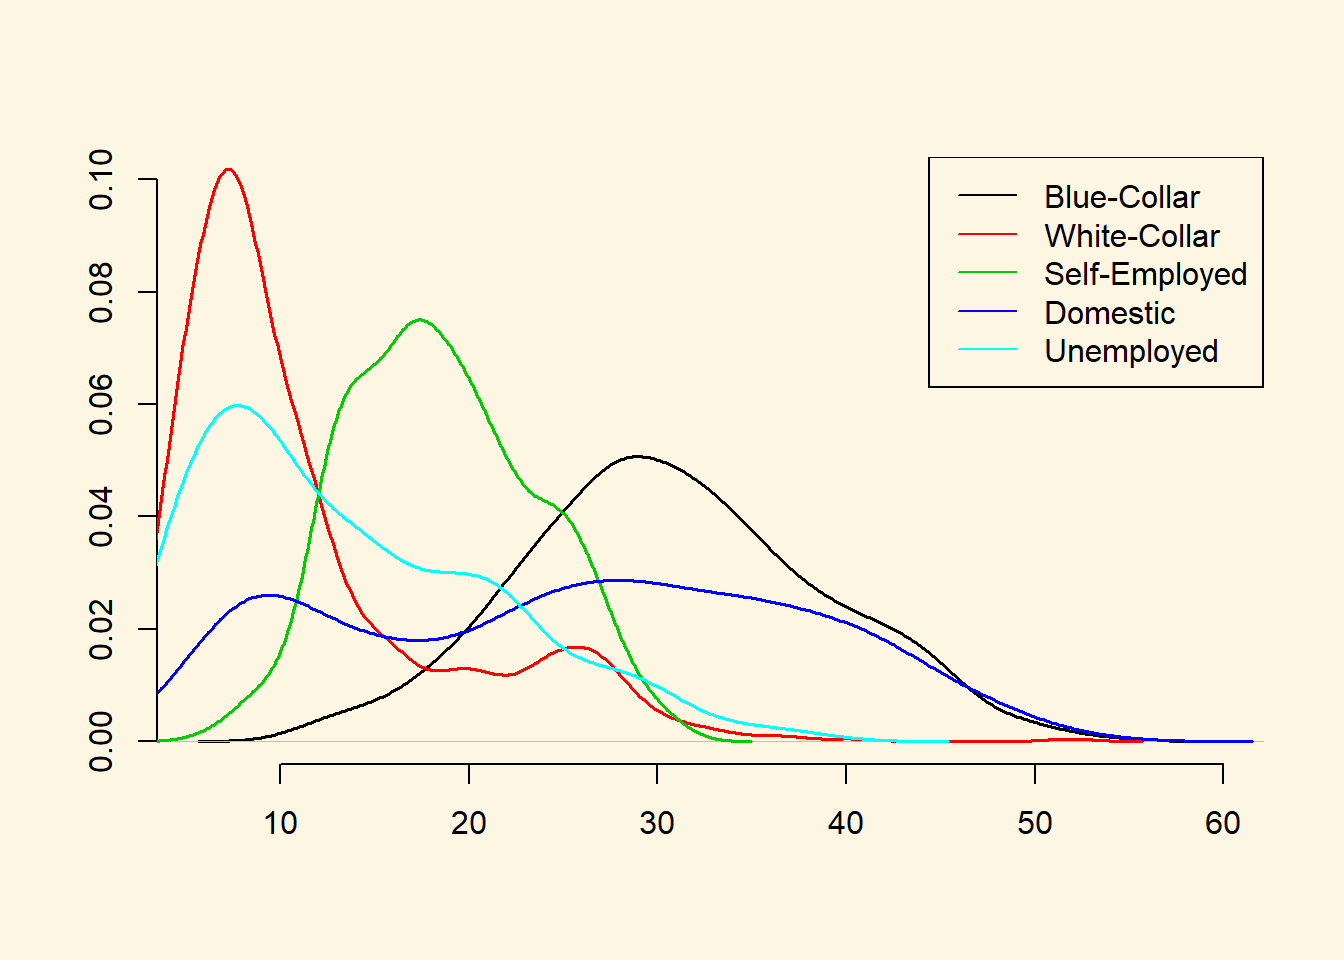
\includegraphics{statistics1_files/figure-latex/unnamed-chunk-270-1.pdf}

\paragraph{Exercise 5}\label{exercise-5-4}

Estimate the mean vote shares for the Nazis in districts where the share
of blue-collar voters was above the mean (30.82) and below it.

\begin{Shaded}
\begin{Highlighting}[]
\CommentTok{# many blue-collar workers}
\NormalTok{share.in.blue.high <-}\StringTok{ }\KeywordTok{mean}\NormalTok{(df}\OperatorTok{$}\NormalTok{sharenazis[ df}\OperatorTok{$}\NormalTok{shareblue }\OperatorTok{>}\StringTok{ }\KeywordTok{mean}\NormalTok{(df}\OperatorTok{$}\NormalTok{shareblue) ])}
\NormalTok{share.in.blue.high}
\end{Highlighting}
\end{Shaded}

\begin{verbatim}
[1] 41.97132
\end{verbatim}

\begin{Shaded}
\begin{Highlighting}[]
\CommentTok{# fewer blue-collar workers}
\NormalTok{share.in.blue.low <-}\StringTok{ }\KeywordTok{mean}\NormalTok{(df}\OperatorTok{$}\NormalTok{sharenazis[ df}\OperatorTok{$}\NormalTok{shareblue }\OperatorTok{<}\StringTok{ }\KeywordTok{mean}\NormalTok{(df}\OperatorTok{$}\NormalTok{shareblue) ])}
\NormalTok{share.in.blue.low}
\end{Highlighting}
\end{Shaded}

\begin{verbatim}
[1] 41.19673
\end{verbatim}

\paragraph{Exercise 6}\label{exercise-6-4}

Construct confidence intervals around the means.

\begin{Shaded}
\begin{Highlighting}[]
\CommentTok{# ci blue-collar workers high}
\NormalTok{se.blue.high <-}\StringTok{ }\KeywordTok{sd}\NormalTok{(df}\OperatorTok{$}\NormalTok{sharenazis[ df}\OperatorTok{$}\NormalTok{shareblue }\OperatorTok{>}\StringTok{ }\KeywordTok{mean}\NormalTok{(df}\OperatorTok{$}\NormalTok{shareblue) ]) }\OperatorTok{/}\StringTok{ }
\StringTok{  }\KeywordTok{sqrt}\NormalTok{( }\KeywordTok{length}\NormalTok{(df}\OperatorTok{$}\NormalTok{sharenazis[ df}\OperatorTok{$}\NormalTok{shareblue }\OperatorTok{>}\StringTok{ }\KeywordTok{mean}\NormalTok{(df}\OperatorTok{$}\NormalTok{shareblue) ]) )}

\CommentTok{# lower bound}
\NormalTok{share.in.blue.high }\OperatorTok{-}\StringTok{ }\FloatTok{1.96} \OperatorTok{*}\StringTok{ }\NormalTok{se.blue.high}
\end{Highlighting}
\end{Shaded}

\begin{verbatim}
[1] 40.90744
\end{verbatim}

\begin{Shaded}
\begin{Highlighting}[]
\CommentTok{# upper bound}
\NormalTok{share.in.blue.high }\OperatorTok{+}\StringTok{ }\FloatTok{1.96} \OperatorTok{*}\StringTok{ }\NormalTok{se.blue.high}
\end{Highlighting}
\end{Shaded}

\begin{verbatim}
[1] 43.03521
\end{verbatim}

\begin{Shaded}
\begin{Highlighting}[]
\CommentTok{# ci blue-collar workers low}
\NormalTok{se.blue.high <-}\StringTok{ }\KeywordTok{sd}\NormalTok{(df}\OperatorTok{$}\NormalTok{sharenazis[ df}\OperatorTok{$}\NormalTok{shareblue }\OperatorTok{<}\StringTok{ }\KeywordTok{mean}\NormalTok{(df}\OperatorTok{$}\NormalTok{shareblue) ]) }\OperatorTok{/}\StringTok{ }
\StringTok{  }\KeywordTok{sqrt}\NormalTok{( }\KeywordTok{length}\NormalTok{(df}\OperatorTok{$}\NormalTok{sharenazis[ df}\OperatorTok{$}\NormalTok{shareblue }\OperatorTok{<}\StringTok{ }\KeywordTok{mean}\NormalTok{(df}\OperatorTok{$}\NormalTok{shareblue) ]) )}

\CommentTok{# lower bound}
\NormalTok{share.in.blue.high }\OperatorTok{-}\StringTok{ }\FloatTok{1.96} \OperatorTok{*}\StringTok{ }\NormalTok{se.blue.high}
\end{Highlighting}
\end{Shaded}

\begin{verbatim}
[1] 40.75962
\end{verbatim}

\begin{Shaded}
\begin{Highlighting}[]
\CommentTok{# upper bound}
\NormalTok{share.in.blue.high }\OperatorTok{+}\StringTok{ }\FloatTok{1.96} \OperatorTok{*}\StringTok{ }\NormalTok{se.blue.high}
\end{Highlighting}
\end{Shaded}

\begin{verbatim}
[1] 43.18303
\end{verbatim}

\paragraph{Exercise 7}\label{exercise-7-3}

Are there differences between the groups? Use the appropriate
statistical test to find out.

\begin{Shaded}
\begin{Highlighting}[]
\CommentTok{# t-test for difference in means}
\KeywordTok{t.test}\NormalTok{(df}\OperatorTok{$}\NormalTok{sharenazis[ df}\OperatorTok{$}\NormalTok{shareblue }\OperatorTok{>}\StringTok{ }\KeywordTok{mean}\NormalTok{(df}\OperatorTok{$}\NormalTok{shareblue) ],}
\NormalTok{       df}\OperatorTok{$}\NormalTok{sharenazis[ df}\OperatorTok{$}\NormalTok{shareblue }\OperatorTok{<}\StringTok{ }\KeywordTok{mean}\NormalTok{(df}\OperatorTok{$}\NormalTok{shareblue) ])}
\end{Highlighting}
\end{Shaded}

\begin{verbatim}

    Welch Two Sample t-test

data:  df$sharenazis[df$shareblue > mean(df$shareblue)] and df$sharenazis[df$shareblue < mean(df$shareblue)]
t = 0.94153, df = 673.93, p-value = 0.3468
alternative hypothesis: true difference in means is not equal to 0
95 percent confidence interval:
 -0.8407583  2.3899379
sample estimates:
mean of x mean of y 
 41.97132  41.19673 
\end{verbatim}

We cannot reject the null hypothesis that there is no difference in
means.

\paragraph{Exercise 8}\label{exercise-8-4}

Calculate t values and p values on your own (without using the t test)

\begin{Shaded}
\begin{Highlighting}[]
\CommentTok{# standard error of the difference in means}
\NormalTok{se.fd <-}\StringTok{ }\KeywordTok{sqrt}\NormalTok{(  (}\KeywordTok{var}\NormalTok{(df}\OperatorTok{$}\NormalTok{sharenazis[ df}\OperatorTok{$}\NormalTok{shareblue }\OperatorTok{>}\StringTok{ }\KeywordTok{mean}\NormalTok{(df}\OperatorTok{$}\NormalTok{shareblue)]) }\OperatorTok{/}\StringTok{ }
\StringTok{                   }\KeywordTok{length}\NormalTok{(df}\OperatorTok{$}\NormalTok{sharenazis[ df}\OperatorTok{$}\NormalTok{shareblue }\OperatorTok{>}\StringTok{ }\KeywordTok{mean}\NormalTok{(df}\OperatorTok{$}\NormalTok{shareblue)])) }\OperatorTok{+}
\StringTok{                  }\NormalTok{(}\KeywordTok{var}\NormalTok{(df}\OperatorTok{$}\NormalTok{sharenazis[ df}\OperatorTok{$}\NormalTok{shareblue }\OperatorTok{<}\StringTok{ }\KeywordTok{mean}\NormalTok{(df}\OperatorTok{$}\NormalTok{shareblue)]) }\OperatorTok{/}\StringTok{ }
\StringTok{                     }\KeywordTok{length}\NormalTok{(df}\OperatorTok{$}\NormalTok{sharenazis[ df}\OperatorTok{$}\NormalTok{shareblue }\OperatorTok{<}\StringTok{ }\KeywordTok{mean}\NormalTok{(df}\OperatorTok{$}\NormalTok{shareblue)])))}

\CommentTok{# t value}
\NormalTok{t.val <-}\StringTok{ }\NormalTok{(share.in.blue.high }\OperatorTok{-}\StringTok{ }\NormalTok{share.in.blue.low) }\OperatorTok{/}\StringTok{ }\NormalTok{se.fd}

\CommentTok{# p value}
\NormalTok{(}\DecValTok{1}\OperatorTok{-}\StringTok{ }\KeywordTok{pnorm}\NormalTok{(t.val))}\OperatorTok{*}\DecValTok{2}
\end{Highlighting}
\end{Shaded}

\begin{verbatim}
[1] 0.3464331
\end{verbatim}

\paragraph{Exercise 9}\label{exercise-9-3}

Interpret your results substantially.

A common hypothesis is that it was blue-collar workers who voted
en-masse for Hitler. However, when comparing districts where the share
of blue-collar workers is above the mean to districts where the share is
below the mean, we do not see any difference in the vote share of Nazis.

Based on this comparison, we would not conclude that a high share of
blue-collar workers made the difference between a good and a bad result
for the National Socialist Party.

\paragraph{Exercise 10}\label{exercise-10-3}

Estimate the mean vote shares for the Nazis in districts where the share
of white-collar voters was above the mean (11.423) and below it.

\begin{Shaded}
\begin{Highlighting}[]
\CommentTok{# clear workspace}
\KeywordTok{rm}\NormalTok{(}\DataTypeTok{list=}\KeywordTok{ls}\NormalTok{())}

\CommentTok{# re-load data}
\NormalTok{df <-}\StringTok{ }\KeywordTok{read.csv}\NormalTok{(}\StringTok{"who_voted_nazi_in_1932.csv"}\NormalTok{)}

\CommentTok{# vector nazi vote share in places where white-collar workers was above the mean}
\NormalTok{n.share.high.wc <-}\StringTok{ }\NormalTok{df}\OperatorTok{$}\NormalTok{sharenazis[ df}\OperatorTok{$}\NormalTok{sharewhite }\OperatorTok{>}\StringTok{ }\KeywordTok{mean}\NormalTok{(df}\OperatorTok{$}\NormalTok{sharewhite) ]}

\CommentTok{# vector nazi vote share in places where white-collar workers was below the mean}
\NormalTok{n.share.low.wc <-}\StringTok{ }\NormalTok{df}\OperatorTok{$}\NormalTok{sharenazis[ df}\OperatorTok{$}\NormalTok{sharewhite }\OperatorTok{<}\StringTok{ }\KeywordTok{mean}\NormalTok{(df}\OperatorTok{$}\NormalTok{sharewhite) ]}

\CommentTok{# high white-collar group mean}
\KeywordTok{mean}\NormalTok{(n.share.high.wc)}
\end{Highlighting}
\end{Shaded}

\begin{verbatim}
[1] 37.83325
\end{verbatim}

\begin{Shaded}
\begin{Highlighting}[]
\CommentTok{# low white-collar group mean}
\KeywordTok{mean}\NormalTok{(n.share.low.wc)}
\end{Highlighting}
\end{Shaded}

\begin{verbatim}
[1] 43.38576
\end{verbatim}

\paragraph{Exercise 11}\label{exercise-11-2}

Construct confidence intervals around the means.

We do this first for the group with a share of white-collar workers.

\begin{Shaded}
\begin{Highlighting}[]
\CommentTok{# number of districts with high white-collar share}
\NormalTok{num.high.wc <-}\StringTok{ }\KeywordTok{length}\NormalTok{(n.share.high.wc)}

\CommentTok{# standard error for high group}
\NormalTok{se.high.wc <-}\StringTok{ }\KeywordTok{sd}\NormalTok{(n.share.high.wc) }\OperatorTok{/}\StringTok{ }\KeywordTok{sqrt}\NormalTok{(num.high.wc)}

\CommentTok{# lower bound}
\KeywordTok{mean}\NormalTok{(n.share.high.wc) }\OperatorTok{-}\StringTok{ }\FloatTok{1.96} \OperatorTok{*}\StringTok{ }\NormalTok{se.high.wc}
\end{Highlighting}
\end{Shaded}

\begin{verbatim}
[1] 36.81174
\end{verbatim}

\begin{Shaded}
\begin{Highlighting}[]
\CommentTok{# upper bound}
\KeywordTok{mean}\NormalTok{(n.share.high.wc) }\OperatorTok{+}\StringTok{ }\FloatTok{1.96} \OperatorTok{*}\StringTok{ }\NormalTok{se.high.wc}
\end{Highlighting}
\end{Shaded}

\begin{verbatim}
[1] 38.85476
\end{verbatim}

Now, we construct the confidence interval around the mean for the group
with a low share of white-collar workers.

\begin{Shaded}
\begin{Highlighting}[]
\CommentTok{# number of districts with low white-collar share}
\NormalTok{num.low.wc <-}\StringTok{ }\KeywordTok{length}\NormalTok{(n.share.low.wc)}

\CommentTok{# standard error for low group}
\NormalTok{se.low.wc <-}\StringTok{ }\KeywordTok{sd}\NormalTok{(n.share.low.wc) }\OperatorTok{/}\StringTok{ }\KeywordTok{sqrt}\NormalTok{(num.low.wc)}

\CommentTok{# lower bound}
\KeywordTok{mean}\NormalTok{(n.share.low.wc) }\OperatorTok{-}\StringTok{ }\FloatTok{1.96} \OperatorTok{*}\StringTok{ }\NormalTok{se.low.wc}
\end{Highlighting}
\end{Shaded}

\begin{verbatim}
[1] 42.32525
\end{verbatim}

\begin{Shaded}
\begin{Highlighting}[]
\CommentTok{# upper bound}
\KeywordTok{mean}\NormalTok{(n.share.low.wc) }\OperatorTok{+}\StringTok{ }\FloatTok{1.96} \OperatorTok{*}\StringTok{ }\NormalTok{se.low.wc}
\end{Highlighting}
\end{Shaded}

\begin{verbatim}
[1] 44.44627
\end{verbatim}

\paragraph{Exercise 12}\label{exercise-12-2}

Are there differences between the groups? Use the appropriate
statistical test to find out.

\begin{Shaded}
\begin{Highlighting}[]
\KeywordTok{t.test}\NormalTok{(n.share.high.wc, n.share.low.wc)}
\end{Highlighting}
\end{Shaded}

\begin{verbatim}

    Welch Two Sample t-test

data:  n.share.high.wc and n.share.low.wc
t = -7.3909, df = 612.69, p-value = 0.0000000000004802
alternative hypothesis: true difference in means is not equal to 0
95 percent confidence interval:
 -7.027862 -4.077152
sample estimates:
mean of x mean of y 
 37.83325  43.38576 
\end{verbatim}

The t test shows that the difference in means is statistically
significant. In districts with a high share of white-collar workers the
share for the Nazis is lower.

\paragraph{Exercise 13}\label{exercise-13-2}

Calculate t values and p values on your own (without using the t test)

\begin{Shaded}
\begin{Highlighting}[]
\CommentTok{# variance in high white-collar group}
\NormalTok{var.high.wc <-}\StringTok{ }\KeywordTok{var}\NormalTok{(n.share.high.wc)}

\CommentTok{# variance in low white-collar group}
\NormalTok{var.low.wc <-}\StringTok{ }\KeywordTok{var}\NormalTok{(n.share.low.wc)}


\CommentTok{# standard error of the difference in means}
\NormalTok{se.fd <-}\StringTok{ }\KeywordTok{sqrt}\NormalTok{( ((var.high.wc}\OperatorTok{/}\NormalTok{num.high.wc) }\OperatorTok{+}\StringTok{ }\NormalTok{(var.low.wc}\OperatorTok{/}\NormalTok{num.low.wc))   )}

\CommentTok{# t value}
\NormalTok{t.val <-}\StringTok{ }\NormalTok{(}\KeywordTok{mean}\NormalTok{(n.share.high.wc) }\OperatorTok{-}\StringTok{ }\KeywordTok{mean}\NormalTok{(n.share.low.wc)) }\OperatorTok{/}\StringTok{ }\NormalTok{se.fd}

\CommentTok{# p value}
\KeywordTok{pnorm}\NormalTok{(t.val) }\OperatorTok{*}\StringTok{ }\DecValTok{2}
\end{Highlighting}
\end{Shaded}

\begin{verbatim}
[1] 0.0000000000001457993
\end{verbatim}

\paragraph{Exercise 14}\label{exercise-14-1}

Interpret your results substantially.

We reject the null hypothesis that there is no difference between
districts with a low share of white-collar workers and districts with a
high share of white-collar workers. In districts where the share of
white-collar workers was high, the share for the Nazis was 5.6
percentage points lower.

\section{Bivariate linear regression
models}\label{bivariate-linear-regression-models}

\subsection{Seminar}\label{seminar-5}

\begin{Shaded}
\begin{Highlighting}[]
\KeywordTok{rm}\NormalTok{(}\DataTypeTok{list =} \KeywordTok{ls}\NormalTok{())}
\end{Highlighting}
\end{Shaded}

\subsubsection{Packages}\label{packages}

We will need to install a package in this week's seminar. Packages are
like apps for your phone. R comes with some core functionality and
allows users to add functionality. These add-ons are called packages. We
first need to install a package (but only once). Every time we start R,
we need to load the package.

To install a package, we write
\texttt{install.packages("package.name")}. To load a package, we write
\texttt{library(package.name)}.

This week's package is called \texttt{texreg} and it makes it easy to
produce publication quality output from our regression models. We'll
discuss this package in more detail as we go along. For now let's
install the package and then load the package.

\begin{Shaded}
\begin{Highlighting}[]
\KeywordTok{install.packages}\NormalTok{(}\StringTok{"texreg"}\NormalTok{) }\CommentTok{# install only once}
\KeywordTok{library}\NormalTok{(texreg) }\CommentTok{# load in the beginning of every R session}
\end{Highlighting}
\end{Shaded}

We will use a dataset collected by the US census bureau that contains
several socioeconomic indicators. You can load the dataset directly from
the internet.

\begin{Shaded}
\begin{Highlighting}[]
\NormalTok{dat <-}\StringTok{ }\KeywordTok{read.csv}\NormalTok{(}\StringTok{"https://raw.githubusercontent.com/philippbroniecki/statistics1/master/data/communities.csv"}\NormalTok{)}
\end{Highlighting}
\end{Shaded}

We will be exploring the relationship between the unemployment rate and
low education. The variable names for these variables are not terribly
clear and so first we will rename these variables using the
\texttt{names()} function and the \texttt{which()} function from last
week.

\begin{Shaded}
\begin{Highlighting}[]
\KeywordTok{names}\NormalTok{(dat)}
\end{Highlighting}
\end{Shaded}

\begin{verbatim}
 [1] "state"           "county"          "community"      
 [4] "communityname"   "fold"            "population"     
 [7] "householdsize"   "racepctblack"    "racePctWhite"   
[10] "racePctAsian"    "racePctHisp"     "agePct12t21"    
[13] "agePct12t29"     "agePct16t24"     "agePct65up"     
[16] "numbUrban"       "pctUrban"        "medIncome"      
[19] "pctWWage"        "pctWFarmSelf"    "pctWInvInc"     
[22] "pctWSocSec"      "pctWPubAsst"     "pctWRetire"     
[25] "medFamInc"       "perCapInc"       "whitePerCap"    
[28] "blackPerCap"     "indianPerCap"    "AsianPerCap"    
[31] "OtherPerCap"     "HispPerCap"      "NumUnderPov"    
[34] "PctPopUnderPov"  "PctLess9thGrade" "PctNotHSGrad"   
[37] "PctBSorMore"     "PctUnemployed"  
\end{verbatim}

\begin{Shaded}
\begin{Highlighting}[]
\KeywordTok{names}\NormalTok{(dat)[}\KeywordTok{which}\NormalTok{(}\KeywordTok{names}\NormalTok{(dat) }\OperatorTok{==}\StringTok{ "PctUnemployed"}\NormalTok{)] <-}\StringTok{ "UnemploymentRate"}
\KeywordTok{names}\NormalTok{(dat)[}\KeywordTok{which}\NormalTok{(}\KeywordTok{names}\NormalTok{(dat) }\OperatorTok{==}\StringTok{ "PctNotHSGrad"}\NormalTok{)] <-}\StringTok{ "NoHighSchool"}
\end{Highlighting}
\end{Shaded}

The first variable (\texttt{UnemploymentRate}) measures the proportion
of citizens in each community who are unemployed. The second variable
(\texttt{NoHighSchool}) measures the proportion of citizens in each
community who failed to finish high-school.

If we summarize these variables with the \texttt{summary()} function, we
will see that they are both measured as proportions (they vary between 0
and 1):

\begin{Shaded}
\begin{Highlighting}[]
\KeywordTok{summary}\NormalTok{(dat}\OperatorTok{$}\NormalTok{UnemploymentRate)}
\end{Highlighting}
\end{Shaded}

\begin{verbatim}
   Min. 1st Qu.  Median    Mean 3rd Qu.    Max. 
 0.0000  0.2200  0.3200  0.3635  0.4800  1.0000 
\end{verbatim}

\begin{Shaded}
\begin{Highlighting}[]
\KeywordTok{summary}\NormalTok{(dat}\OperatorTok{$}\NormalTok{NoHighSchool)}
\end{Highlighting}
\end{Shaded}

\begin{verbatim}
   Min. 1st Qu.  Median    Mean 3rd Qu.    Max. 
 0.0000  0.2300  0.3600  0.3833  0.5100  1.0000 
\end{verbatim}

It will be a little easier to interpret the regression output if we
convert these to percentages rather than proportions. We can do this
with the following lines of code:

\begin{Shaded}
\begin{Highlighting}[]
\NormalTok{dat}\OperatorTok{$}\NormalTok{UnemploymentRate <-}\StringTok{ }\NormalTok{dat}\OperatorTok{$}\NormalTok{UnemploymentRate}\OperatorTok{*}\DecValTok{100}
\NormalTok{dat}\OperatorTok{$}\NormalTok{NoHighSchool <-}\StringTok{ }\NormalTok{dat}\OperatorTok{$}\NormalTok{NoHighSchool}\OperatorTok{*}\DecValTok{100}
\end{Highlighting}
\end{Shaded}

We can begin by drawing a scatterplot with the percentage of unemployed
people on the y-axis and the percentage of adults without high-school
education on the x-axis.

\begin{Shaded}
\begin{Highlighting}[]
\KeywordTok{plot}\NormalTok{(}
  \DataTypeTok{y =}\NormalTok{ dat}\OperatorTok{$}\NormalTok{UnemploymentRate,}
  \DataTypeTok{x =}\NormalTok{ dat}\OperatorTok{$}\NormalTok{NoHighSchool, }
  \DataTypeTok{xlab =} \StringTok{"Adults without High School education (%)"}\NormalTok{,}
  \DataTypeTok{ylab =} \StringTok{"Unemployment (%)"}\NormalTok{,}
  \DataTypeTok{bty =} \StringTok{"n"}\NormalTok{,}
  \DataTypeTok{pch =} \DecValTok{16}\NormalTok{,}
  \DataTypeTok{col =} \KeywordTok{rgb}\NormalTok{(}\DataTypeTok{red =} \DecValTok{110}\NormalTok{, }\DataTypeTok{green =} \DecValTok{200}\NormalTok{, }\DataTypeTok{blue =} \DecValTok{110}\NormalTok{, }\DataTypeTok{alpha =} \DecValTok{80}\NormalTok{, }\DataTypeTok{maxColorValue =} \DecValTok{255}\NormalTok{)}
\NormalTok{)}
\end{Highlighting}
\end{Shaded}

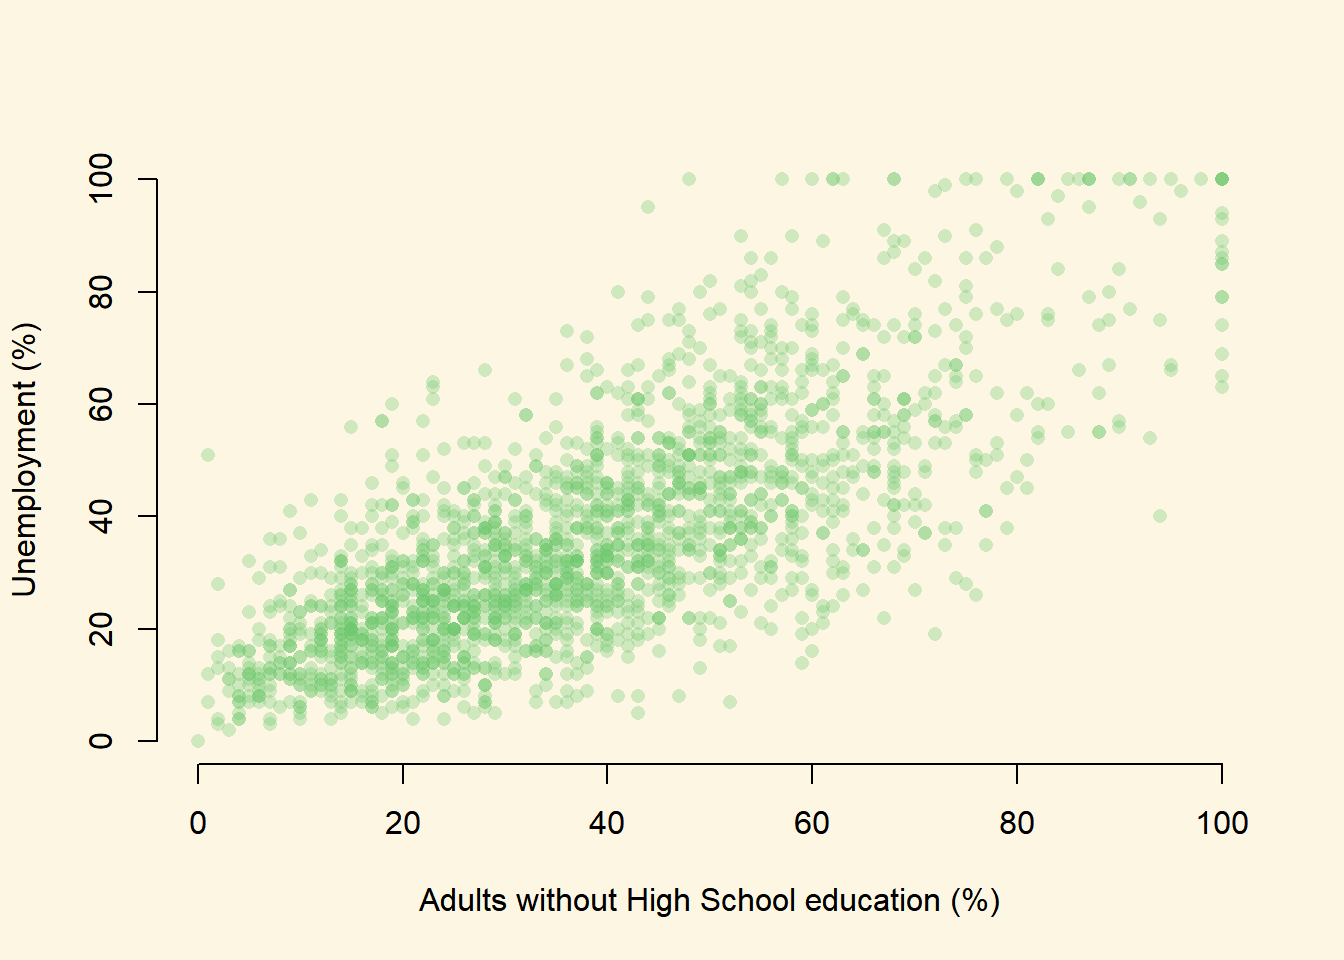
\includegraphics{statistics1_files/figure-latex/unnamed-chunk-289-1.pdf}

From looking at the plot, what is the association between the
unemployment rate and lack of high-school level education?

In order to answer that question empirically, we will run a linear
regression using the \href{http://bit.ly/R_lm}{\texttt{lm()}} function
in R. The \href{http://bit.ly/R_lm}{\texttt{lm()}} function needs to
know a) the relationship we're trying to model and b) the dataset for
our observations. The two arguments we need to provide to the
\href{http://bit.ly/R_lm}{\texttt{lm()}} function are described below.

\begin{longtable}[]{@{}ll@{}}
\toprule
\begin{minipage}[b]{0.12\columnwidth}\raggedright\strut
Argument\strut
\end{minipage} & \begin{minipage}[b]{0.78\columnwidth}\raggedright\strut
Description\strut
\end{minipage}\tabularnewline
\midrule
\endhead
\begin{minipage}[t]{0.12\columnwidth}\raggedright\strut
\texttt{formula}\strut
\end{minipage} & \begin{minipage}[t]{0.78\columnwidth}\raggedright\strut
The \texttt{formula} describes the relationship between the dependent
and independent variables, for example
\texttt{dependent.variable\ \textasciitilde{}\ independent.variable} In
our case, we'd like to model the relationship using the formula:
\texttt{UnemploymentRate\ \textasciitilde{}\ NoHighSchool}\strut
\end{minipage}\tabularnewline
\begin{minipage}[t]{0.12\columnwidth}\raggedright\strut
\texttt{data}\strut
\end{minipage} & \begin{minipage}[t]{0.78\columnwidth}\raggedright\strut
This is simply the name of the dataset that contains the variable of
interest. In our case, this is the merged dataset called
\texttt{communities}.\strut
\end{minipage}\tabularnewline
\bottomrule
\end{longtable}

For more information on how the \texttt{lm()} function works, type
help(lm) in R.

\begin{Shaded}
\begin{Highlighting}[]
\NormalTok{model1 <-}\StringTok{ }\KeywordTok{lm}\NormalTok{(UnemploymentRate }\OperatorTok{~}\StringTok{ }\NormalTok{NoHighSchool, }\DataTypeTok{data =}\NormalTok{ dat)}
\end{Highlighting}
\end{Shaded}

The \href{http://bit.ly/R_lm}{\texttt{lm()}} function has modeled the
relationship between \texttt{PctUnemployed} and \texttt{NoHighSchool}
and we've saved it in an object called \texttt{model1}. Let's use the
\href{http://bit.ly/R_summary}{\texttt{summary()}} function to see what
this linear model looks like.

\begin{Shaded}
\begin{Highlighting}[]
\KeywordTok{summary}\NormalTok{(model1)}
\end{Highlighting}
\end{Shaded}

\begin{verbatim}

Call:
lm(formula = UnemploymentRate ~ NoHighSchool, data = dat)

Residuals:
    Min      1Q  Median      3Q     Max 
-42.347  -8.499  -1.189   7.711  56.470 

Coefficients:
             Estimate Std. Error t value            Pr(>|t|)    
(Intercept)   7.89520    0.64833   12.18 <0.0000000000000002 ***
NoHighSchool  0.74239    0.01496   49.64 <0.0000000000000002 ***
---
Signif. codes:  0 '***' 0.001 '**' 0.01 '*' 0.05 '.' 0.1 ' ' 1

Residual standard error: 13.52 on 1992 degrees of freedom
Multiple R-squared:  0.553, Adjusted R-squared:  0.5527 
F-statistic:  2464 on 1 and 1992 DF,  p-value: < 0.00000000000000022
\end{verbatim}

\paragraph{Interpreting Regression
Output}\label{interpreting-regression-output}

The output from \href{http://bit.ly/R_lm}{\texttt{lm()}} might seem
overwhelming at first so let's break it down one item at a time.

\begin{figure}
\centering
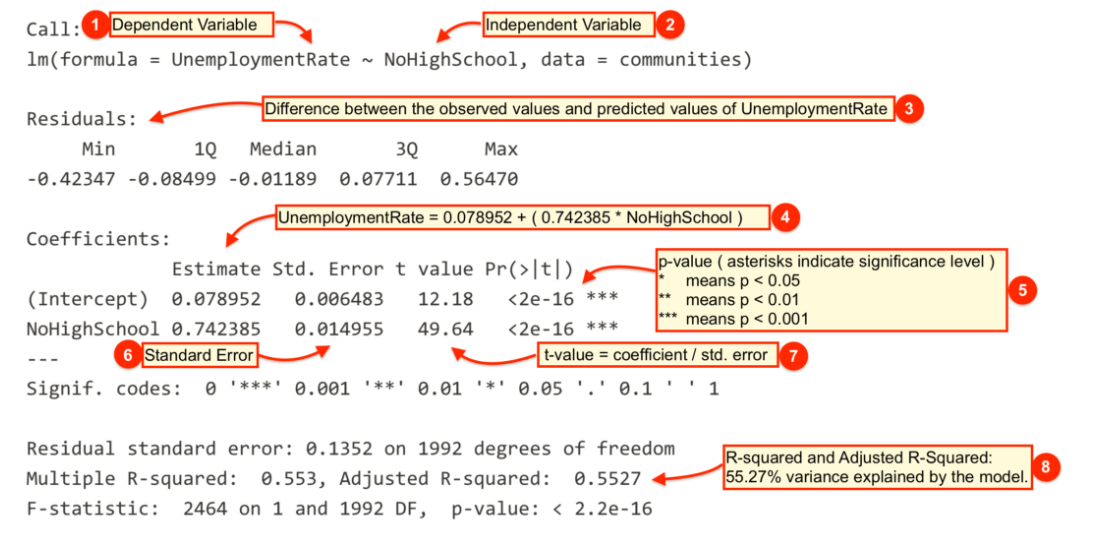
\includegraphics{./img/lm.png}
\caption{}
\end{figure}

\begin{longtable}[]{@{}ll@{}}
\toprule
\begin{minipage}[b]{0.08\columnwidth}\raggedright\strut
\#\strut
\end{minipage} & \begin{minipage}[b]{0.86\columnwidth}\raggedright\strut
Description\strut
\end{minipage}\tabularnewline
\midrule
\endhead
\begin{minipage}[t]{0.08\columnwidth}\raggedright\strut

\includegraphics[width=1.00000\textwidth]{./img/circle1.png}\strut
\end{minipage} & \begin{minipage}[t]{0.86\columnwidth}\raggedright\strut
The \emph{dependent} variable, also sometimes called the outcome
variable. We are trying to model the effects of \texttt{NoHighSchool} on
\texttt{UnemploymentRate} so \texttt{UnemploymentRate} is the
\emph{dependent} variable.\strut
\end{minipage}\tabularnewline
\begin{minipage}[t]{0.08\columnwidth}\raggedright\strut

\includegraphics[width=1.00000\textwidth]{./img/circle2.png}\strut
\end{minipage} & \begin{minipage}[t]{0.86\columnwidth}\raggedright\strut
The \emph{independent} variable or the predictor variable. In our
example, \texttt{NoHighSchool} is the \emph{independent} variable.\strut
\end{minipage}\tabularnewline
\begin{minipage}[t]{0.08\columnwidth}\raggedright\strut

\includegraphics[width=1.00000\textwidth]{./img/circle3.png}\strut
\end{minipage} & \begin{minipage}[t]{0.86\columnwidth}\raggedright\strut
The differences between the observed values and the predicted values are
called \emph{residuals}. R produces a summary of the residuals.\strut
\end{minipage}\tabularnewline
\begin{minipage}[t]{0.08\columnwidth}\raggedright\strut

\includegraphics[width=1.00000\textwidth]{./img/circle4.png}\strut
\end{minipage} & \begin{minipage}[t]{0.86\columnwidth}\raggedright\strut
The \emph{coefficients} for the intercept and the \emph{independent}
variables. Using the \emph{coefficients} we can write down the
relationship between the \emph{dependent} and the \emph{independent}
variables as: \texttt{UnemploymentRate} = 7.8952023 + ( 0.7423853 *
\texttt{NoHighSchool} ) This tells us that for each unit increase in the
variable \texttt{NoHighSchool}, the \texttt{UnemploymentRate} increases
by 0.7423853.\strut
\end{minipage}\tabularnewline
\begin{minipage}[t]{0.08\columnwidth}\raggedright\strut

\includegraphics[width=1.00000\textwidth]{./img/circle5.png}\strut
\end{minipage} & \begin{minipage}[t]{0.86\columnwidth}\raggedright\strut
The \emph{p-value} for each of the coefficients in the model. Recall
that according to the null hypotheses, the value of the coefficient of
interest is zero. The \emph{p-value} tells us whether can can reject the
null hypotheses or not.\strut
\end{minipage}\tabularnewline
\begin{minipage}[t]{0.08\columnwidth}\raggedright\strut

\includegraphics[width=1.00000\textwidth]{./img/circle6.png}\strut
\end{minipage} & \begin{minipage}[t]{0.86\columnwidth}\raggedright\strut
The \emph{standard error} estimates the standard deviation of the
sampling distribution of the coefficients in our model. We can think of
the \emph{standard error} as the measure of precision for the estimated
coefficients.\strut
\end{minipage}\tabularnewline
\begin{minipage}[t]{0.08\columnwidth}\raggedright\strut

\includegraphics[width=1.00000\textwidth]{./img/circle7.png}\strut
\end{minipage} & \begin{minipage}[t]{0.86\columnwidth}\raggedright\strut
The \emph{t statistic} is obtained by dividing the \emph{coefficients}
by the \emph{standard error}.\strut
\end{minipage}\tabularnewline
\begin{minipage}[t]{0.08\columnwidth}\raggedright\strut

\includegraphics[width=1.00000\textwidth]{./img/circle8.png}\strut
\end{minipage} & \begin{minipage}[t]{0.86\columnwidth}\raggedright\strut
The \emph{R-squared} and \emph{adjusted R-squared} tell us how much of
the variance in our model is accounted for by the \emph{independent}
variable. The \emph{adjusted R-squared} is always smaller than
\emph{R-squared} as it takes into account the number of
\emph{independent} variables and degrees of freedom.\strut
\end{minipage}\tabularnewline
\bottomrule
\end{longtable}

Now let's add a regression line to the scatter plot using the
\href{http://bit.ly/R_abline}{\texttt{abline()}} function.

\begin{Shaded}
\begin{Highlighting}[]
\NormalTok{## First we run the same "plot" function as before}
\KeywordTok{plot}\NormalTok{(}
\NormalTok{  UnemploymentRate }\OperatorTok{~}\StringTok{ }\NormalTok{NoHighSchool, }\DataTypeTok{data =}\NormalTok{ dat,}
  \DataTypeTok{xlab =} \StringTok{"Adults without High School education (%)"}\NormalTok{,}
  \DataTypeTok{ylab =} \StringTok{"Unemployment (%)"}\NormalTok{,}
  \DataTypeTok{frame.plot =} \OtherTok{FALSE}\NormalTok{,}
  \DataTypeTok{pch =} \DecValTok{16}\NormalTok{,}
  \DataTypeTok{col =} \KeywordTok{rgb}\NormalTok{(}\DataTypeTok{red =} \DecValTok{110}\NormalTok{, }\DataTypeTok{green =} \DecValTok{200}\NormalTok{, }\DataTypeTok{blue =} \DecValTok{110}\NormalTok{, }\DataTypeTok{alpha =} \DecValTok{80}\NormalTok{, }\DataTypeTok{maxColorValue =} \DecValTok{255}\NormalTok{)}
\NormalTok{)}

\NormalTok{## Then we use the "abline" function to plot the regression line from our saved model object}
\KeywordTok{abline}\NormalTok{(model1, }\DataTypeTok{lwd =} \DecValTok{3}\NormalTok{,}
       \DataTypeTok{col =} \KeywordTok{rgb}\NormalTok{(}\DataTypeTok{red =} \DecValTok{230}\NormalTok{, }\DataTypeTok{green =} \DecValTok{150}\NormalTok{, }\DataTypeTok{blue =} \DecValTok{0}\NormalTok{, }\DataTypeTok{alpha =} \DecValTok{255}\NormalTok{, }\DataTypeTok{maxColorValue =} \DecValTok{255}\NormalTok{))}
\end{Highlighting}
\end{Shaded}

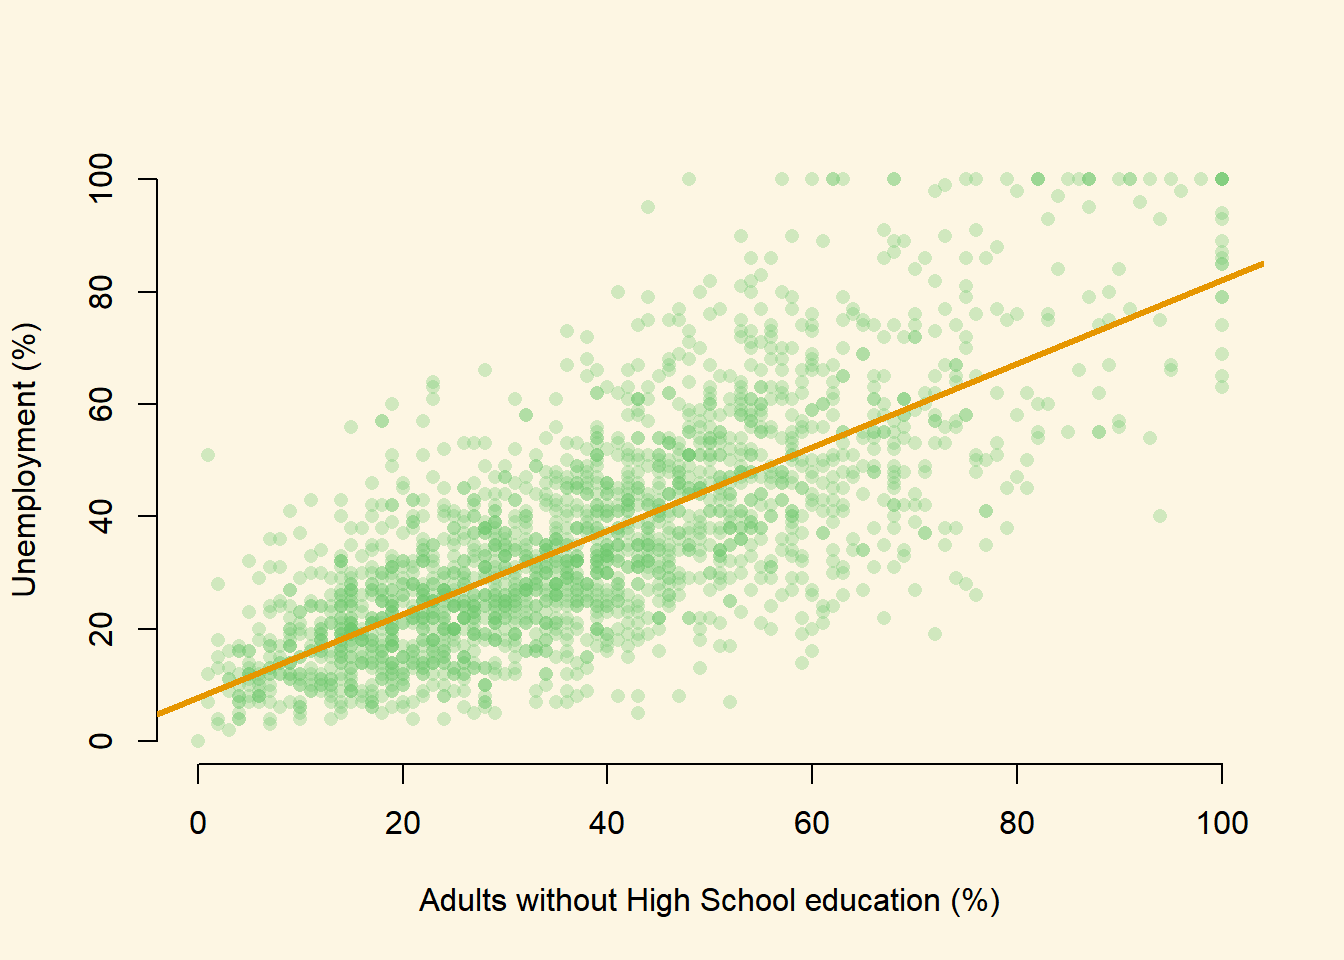
\includegraphics{statistics1_files/figure-latex/unnamed-chunk-292-1.pdf}

We can see by looking at the regression line that it matches the
coefficients we estimated above. For example, when \texttt{NoHighSchool}
is equal to zero (i.e.~where the line intersects the Y-axis), the
predicted value for \texttt{UnemploymentRate} seems to be above 0 but
below 10. This is good, as the \emph{intercept} coefficient we estimated
in the regression was \texttt{7.895}.

Similarly, the coefficient for the variable \texttt{NoHighSchool} was
estimated to be \texttt{0.74239}, which implies that a one point
increase in the percentage of citizens with no high-school education is
associated with about .74 of a point increase in the percentage of
citizens who are unemployed. The line in the plot seems to reflect this:
it is upward sloping, so that higher levels of the no high-school
variable are associated with higher levels of unemployment, but the
relationship is not quite 1-to-1. That is, for each additional
percentage point of citzens without high school education, the
percentage of citizens who are unemployed increases by a little less
than one point.

While the \href{http://bit.ly/R_summary}{\texttt{summary()}} function
provides a slew of information about a fitted regression model, we often
need to present our findings in easy to read tables similar to what you
see in journal publications. The \texttt{texreg} package we installed
earlier allows us to do just that.

Let's take a look at how to display the output of a regression model on
the screen using the \href{http://bit.ly/R_texreg}{\texttt{screenreg()}}
function from \texttt{texreg}.

\begin{Shaded}
\begin{Highlighting}[]
\KeywordTok{screenreg}\NormalTok{(model1)}
\end{Highlighting}
\end{Shaded}

\begin{verbatim}

=========================
              Model 1    
-------------------------
(Intercept)      7.90 ***
                (0.65)   
NoHighSchool     0.74 ***
                (0.01)   
-------------------------
R^2              0.55    
Adj. R^2         0.55    
Num. obs.     1994       
RMSE            13.52    
=========================
*** p < 0.001, ** p < 0.01, * p < 0.05
\end{verbatim}

Here, the output includes some of the most salient details we need for
interpretation. We can see the coefficient for the \texttt{NoHighSchool}
variable, and the estimated coefficient for the intercept. Below these
numbers, in brackets, we can see the standard errors. The table also
reports the R\^{}2, the adjusted R\^{}2, the number of observations (n)
and the root-mean-squared-error (RMSE).

One thing to note is that the table does not include either t-statistics
or p-values for the estimated coefficents. Instead, the table employs a
common device of using stars to denote whether a variable is
statistically significant at a given alpha level.

\begin{itemize}
\tightlist
\item
  \texttt{***} indicates that the coefficient is significant at the
  99.9\% confidence level (alpha = 0.001)
\item
  \texttt{**} indicates that the coefficient is significant at the 99\%
  confidence level (alpha = 0.01)
\item
  \texttt{*} indicates that the coefficient is significant at the 95\%
  confidence level (alpha = 0.05)
\end{itemize}

Returning to our example, are there other variables that might affect
the unemployment rate in our dataset? For example, is the unemployment
rate higher in rural areas? To answer this question, we can swap
\texttt{NoHighSchool} for a different independent variable. Let's use
the variable \texttt{population}, which measures the proportion of
adults who live in cities (rather than rural areas). Again, we can
transform this proportion to a percentage with the following code:

\begin{Shaded}
\begin{Highlighting}[]
\NormalTok{dat}\OperatorTok{$}\NormalTok{population <-}\StringTok{ }\NormalTok{dat}\OperatorTok{$}\NormalTok{population}\OperatorTok{*}\DecValTok{100}
\end{Highlighting}
\end{Shaded}

Let's fit a linear model using \texttt{population} as the independent
variable:

\begin{Shaded}
\begin{Highlighting}[]
\NormalTok{model2 <-}\StringTok{ }\KeywordTok{lm}\NormalTok{(UnemploymentRate }\OperatorTok{~}\StringTok{ }\NormalTok{population, }\DataTypeTok{data =}\NormalTok{ dat)}
\KeywordTok{summary}\NormalTok{(model2)}
\end{Highlighting}
\end{Shaded}

\begin{verbatim}

Call:
lm(formula = UnemploymentRate ~ population, data = dat)

Residuals:
    Min      1Q  Median      3Q     Max 
-35.252 -14.715  -3.946  11.054  64.980 

Coefficients:
            Estimate Std. Error t value             Pr(>|t|)    
(Intercept) 35.02042    0.49206  71.171 < 0.0000000000000002 ***
population   0.23139    0.03532   6.552       0.000000000072 ***
---
Signif. codes:  0 '***' 0.001 '**' 0.01 '*' 0.05 '.' 0.1 ' ' 1

Residual standard error: 20.01 on 1992 degrees of freedom
Multiple R-squared:  0.0211,    Adjusted R-squared:  0.02061 
F-statistic: 42.93 on 1 and 1992 DF,  p-value: 0.00000000007201
\end{verbatim}

We can show regression line from the \texttt{model2} just like we did
with our first model.

\begin{Shaded}
\begin{Highlighting}[]
\KeywordTok{plot}\NormalTok{(}
\NormalTok{  UnemploymentRate }\OperatorTok{~}\StringTok{ }\NormalTok{population, }\DataTypeTok{data =}\NormalTok{ dat,}
  \DataTypeTok{xlab =} \StringTok{"Adults living in cities (%)"}\NormalTok{,}
  \DataTypeTok{ylab =} \StringTok{"unemployment (%)"}\NormalTok{,}
  \DataTypeTok{frame.plot =} \OtherTok{FALSE}\NormalTok{,}
  \DataTypeTok{pch =} \DecValTok{16}\NormalTok{,}
  \DataTypeTok{col =} \KeywordTok{rgb}\NormalTok{(}\DataTypeTok{red =} \DecValTok{110}\NormalTok{, }\DataTypeTok{green =} \DecValTok{200}\NormalTok{, }\DataTypeTok{blue =} \DecValTok{110}\NormalTok{, }\DataTypeTok{alpha =} \DecValTok{100}\NormalTok{, }\DataTypeTok{maxColorValue =} \DecValTok{255}\NormalTok{)}
\NormalTok{  )}
\KeywordTok{abline}\NormalTok{(model2, }\DataTypeTok{lwd =} \DecValTok{2}\NormalTok{,}
       \DataTypeTok{col =} \KeywordTok{rgb}\NormalTok{(}\DataTypeTok{red =} \DecValTok{230}\NormalTok{, }\DataTypeTok{green =} \DecValTok{150}\NormalTok{, }\DataTypeTok{blue =} \DecValTok{0}\NormalTok{, }\DataTypeTok{alpha =} \DecValTok{255}\NormalTok{, }\DataTypeTok{maxColorValue =} \DecValTok{255}\NormalTok{))}
\end{Highlighting}
\end{Shaded}

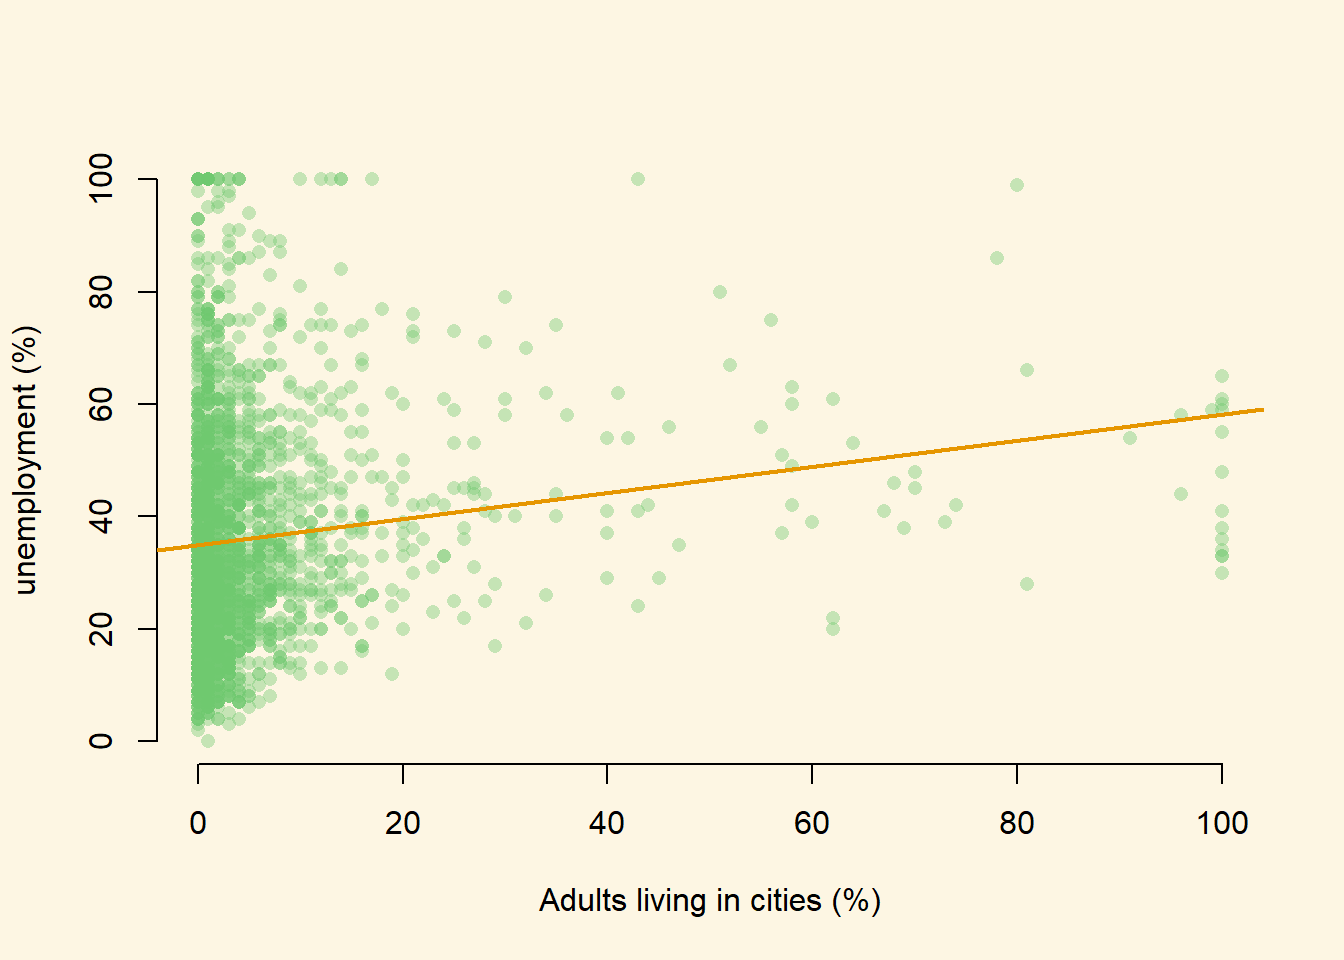
\includegraphics{statistics1_files/figure-latex/unnamed-chunk-296-1.pdf}

So we now have two models! Often, we will want to compare two estimated
models side-by-side. We might want to say how the coefficients for the
independent variables we included differ in \texttt{model1} and
\texttt{model2}, for example. Or we may want to ask: Does
\texttt{model2} offer a better fit than \texttt{model1}?

It is often useful to print the salient details from the estimated
models side-by-side. We can do this by using the
\href{http://bit.ly/R_texreg}{\texttt{screenreg()}} function.

\begin{Shaded}
\begin{Highlighting}[]
\KeywordTok{screenreg}\NormalTok{(}\KeywordTok{list}\NormalTok{(model1, model2))}
\end{Highlighting}
\end{Shaded}

\begin{verbatim}

======================================
              Model 1      Model 2    
--------------------------------------
(Intercept)      7.90 ***    35.02 ***
                (0.65)       (0.49)   
NoHighSchool     0.74 ***             
                (0.01)                
population                    0.23 ***
                             (0.04)   
--------------------------------------
R^2              0.55         0.02    
Adj. R^2         0.55         0.02    
Num. obs.     1994         1994       
RMSE            13.52        20.01    
======================================
*** p < 0.001, ** p < 0.01, * p < 0.05
\end{verbatim}

What does this table tell us?

\begin{itemize}
\tightlist
\item
  The first column replicates the results from our first model. We can
  see that a one point increase in the percentage of citizens without
  high-school education is associated with an increase of 0.74
  percentage points of unemployment, on average.
\item
  The second column gives us the results from the second model. Here, a
  one point increase in the percentage of citizens who live in cities is
  associated with an increase of 0.23 percentage points of unemployment,
  on average
\item
  We can also compare the R\^{}2 values from the two models. The R\^{}2
  for \texttt{model1} is 0.55 and for \texttt{model2} is 0.02. This
  suggests that the model with \texttt{NoHighSchool} as the explanatory
  variable explains about 55\% of the variation in unemployment. The
  model with \texttt{population} as the explanatory variable, on the
  other hand, explains just 2\% of the variation in unemployment.
\end{itemize}

Finally, and this is something that might help with your coursework,
let's save the same output as a Microsoft Word document using
\href{http://bit.ly/R_texreg}{\texttt{htmlreg()}}.

\begin{Shaded}
\begin{Highlighting}[]
\KeywordTok{htmlreg}\NormalTok{(}\KeywordTok{list}\NormalTok{(model1, model2), }\DataTypeTok{file =} \StringTok{"Regressions_on_Unemployment.doc"}\NormalTok{)}
\end{Highlighting}
\end{Shaded}

\subsubsection{Fitted values}\label{fitted-values}

Once we have estimated a regression model, we can use that model to
produce fitted values. Fitted values represent our ``best guess'' for
the value of our dependent variable for a specific value of our
independent variable.

To calculate fitted values we use the \texttt{predict()} function. Let's
say that, on the basis of \texttt{model1} we would like to know what the
unemployment rate is likely to be for a community where the percentage
of adults without a high-school education is equal to 10\%.

The predict function takes two main arguments.

\begin{longtable}[]{@{}ll@{}}
\toprule
\begin{minipage}[b]{0.12\columnwidth}\raggedright\strut
Argument\strut
\end{minipage} & \begin{minipage}[b]{0.78\columnwidth}\raggedright\strut
Description\strut
\end{minipage}\tabularnewline
\midrule
\endhead
\begin{minipage}[t]{0.12\columnwidth}\raggedright\strut
\texttt{object}\strut
\end{minipage} & \begin{minipage}[t]{0.78\columnwidth}\raggedright\strut
The \texttt{object} is the model object that we would like to use to
produce fitted values. Here, we would like to base the analysis on
\texttt{model1} and so specify \texttt{object\ =\ model1} here.\strut
\end{minipage}\tabularnewline
\begin{minipage}[t]{0.12\columnwidth}\raggedright\strut
\texttt{newdata}\strut
\end{minipage} & \begin{minipage}[t]{0.78\columnwidth}\raggedright\strut
This is an optional argument which we use to specify the values of our
independent variable(s) that we would like fitted values for. If we
leave this argument empty, R will automatically calculate fitted values
for all of the observations in the data that we used to estimate the
original model. If we include this argument, we need to provide a
\texttt{data.frame} which has a variable with the same name as the
independent variable in our model. Here, we specify
\texttt{newdata\ =\ data.frame(NoHighSchool\ =\ 10)}, as we would like
the fitted value for a community where 10\% of adults did not complete
high-school.\strut
\end{minipage}\tabularnewline
\bottomrule
\end{longtable}

\begin{Shaded}
\begin{Highlighting}[]
\KeywordTok{predict}\NormalTok{(model1, }\DataTypeTok{newdata =} \KeywordTok{data.frame}\NormalTok{(}\DataTypeTok{NoHighSchool =} \DecValTok{10}\NormalTok{))}
\end{Highlighting}
\end{Shaded}

\begin{verbatim}
       1 
15.31906 
\end{verbatim}

Note that in this simple case, we can calculate the fitted value
manually. The fitted value formula is:

\[\hat{Y}_{i} = \hat{\beta}_0 + \hat{\beta}_1 * X_i\]

So, we can substitute in the relevant coefficients from \texttt{model1}
and the number 10 for our X variable (as we want a fitted value for when
X is equal to 10), and we get:

\[\hat{Y}_{i} = 7.9 + 0.74 * 10 = 15.3\]

which is the same as the result we obtained from the \texttt{predict()}
function! The good thing about the \texttt{predict()} function, however,
is that we will be able to use it for \emph{all} the models we study on
this course, and it can be useful for calculating many different fitted
values. This will save a lot of time which might be wasted doing the
calculations by hand.

\subsubsection{Additional Resources}\label{additional-resources}

\begin{itemize}
\tightlist
\item
  \href{http://altaf.shinyapps.io/linear-regression}{Linear Regression -
  Interactive App}
\end{itemize}

\subsubsection{Exercises}\label{exercises-5}

\begin{enumerate}
\def\labelenumi{\arabic{enumi}.}
\tightlist
\item
  Open a new script and save it as assignment6.
\item
  Clear your workspace.
\item
  Load the non-western foreigners dataset from week 2.
\item
  Estimate a model that explains subjective number of immigrants per 100
  British citizens using only one independent variable. Justify your
  choice. (You do not have to pick the best variable but try to make a
  reasonable argument why more of x should lead to more/less of y).
\item
  Plot a scatterplot of the relationship and add the regression line to
  the plot.
\item
  Interpret the regression output and try to imagine that you are
  communicating your results to someone who does not know anything about
  statistics.
\item
  Estimate another model (i.e.~choose a different independent variable)
  on the same dependent variable. Justify the choice.
\item
  Interpret the new regression output.
\item
  Compare the two models and explain which one you would choose.
\item
  Produce a table with both models next to each other in some text
  document. You can use \texttt{texreg} from the seminar, do it
  manually, or use something else.
\item
  Consider the following table. This analysis asks whether individuals
  who have spent longer in education have higher yearly earnings. The
  analysis is based on a sample of 300 individuals. The dependent
  variable in this analysis is the yearly income of the individual in UK
  pounds (\texttt{earnings}). The independent variable measures the
  number of years the individual spent in full-time education
  (\texttt{education}).
\end{enumerate}

\begin{itemize}
\tightlist
\item
  Interpret the coefficient on the \texttt{education} variable.
\item
  Using the values given in the table, calculate the test-statistic
\item
  Can we reject the null hypothesis of no effect at the 95\% confidence
  level? (Just looking at the stars is not sufficient here! How can we
  work out the result of the hypothesis test?)
\end{itemize}

\begin{verbatim}

=========================
             Model 1     
-------------------------
(Intercept)   3663.85    
             (2326.99)   
education     1270.81 ***
              (160.97)   
-------------------------
R^2              0.17    
Adj. R^2         0.17    
Num. obs.      300       
RMSE         14018.52    
=========================
*** p < 0.001, ** p < 0.01, * p < 0.05
\end{verbatim}

\begin{enumerate}
\def\labelenumi{\arabic{enumi}.}
\setcounter{enumi}{11}
\tightlist
\item
  Save the script that includes all previous tasks.
\item
  Source your script, i.e.~run the entire script all at once without
  error message.
\end{enumerate}

\subsection{Solutions}\label{solutions-5}

\paragraph{Exercise 3}\label{exercise-3-5}

Load the non-western foreigners dataset from week 2.

\begin{Shaded}
\begin{Highlighting}[]
\KeywordTok{load}\NormalTok{(}\StringTok{"BSAS_manip.RData"}\NormalTok{)}
\end{Highlighting}
\end{Shaded}

\paragraph{Exercise 4}\label{exercise-4-5}

Estimate a model that explains subjective number of immigrants per 100
British citizens using only one independent variable. Justify your
choice. (You do not have to pick the best variable but try to make a
reasonable argument why more of x should lead to more/less of y).

\begin{Shaded}
\begin{Highlighting}[]
\NormalTok{m1 <-}\StringTok{ }\KeywordTok{lm}\NormalTok{(IMMBRIT }\OperatorTok{~}\StringTok{ }\NormalTok{RAge, }\DataTypeTok{data =}\NormalTok{ data2)}
\end{Highlighting}
\end{Shaded}

We use age as predictor variable. We argue that older people are less
positive towards immigration and tend to overestimate the number of
immigrants to overemphasize the problem. We, therefore, expect a
positive relationship between age and the perception of immigration.

\paragraph{Exercise 5}\label{exercise-5-5}

Plot a scatterplot of the relationship and add the regression line to
the plot.

\begin{Shaded}
\begin{Highlighting}[]
\KeywordTok{plot}\NormalTok{(}
  \DataTypeTok{y =}\NormalTok{ data2}\OperatorTok{$}\NormalTok{IMMBRIT,}
  \DataTypeTok{x =}\NormalTok{ data2}\OperatorTok{$}\NormalTok{RAge,}
  \DataTypeTok{xlab =} \StringTok{"age"}\NormalTok{,}
  \DataTypeTok{ylab =} \StringTok{"immigration perception"}\NormalTok{,}
  \DataTypeTok{frame.plot =} \OtherTok{FALSE}\NormalTok{,}
  \DataTypeTok{pch =} \DecValTok{16}\NormalTok{,}
  \DataTypeTok{col =} \KeywordTok{rgb}\NormalTok{(}\DataTypeTok{red =} \DecValTok{110}\NormalTok{, }\DataTypeTok{green =} \DecValTok{200}\NormalTok{, }\DataTypeTok{blue =} \DecValTok{110}\NormalTok{, }\DataTypeTok{alpha =} \DecValTok{80}\NormalTok{, }\DataTypeTok{maxColorValue =} \DecValTok{255}\NormalTok{)}
\NormalTok{)}
\KeywordTok{abline}\NormalTok{(m1, }\DataTypeTok{lwd =} \DecValTok{3}\NormalTok{,}
       \DataTypeTok{col =} \KeywordTok{rgb}\NormalTok{(}\DataTypeTok{red =} \DecValTok{230}\NormalTok{, }\DataTypeTok{green =} \DecValTok{150}\NormalTok{, }\DataTypeTok{blue =} \DecValTok{0}\NormalTok{, }\DataTypeTok{alpha =} \DecValTok{255}\NormalTok{, }\DataTypeTok{maxColorValue =} \DecValTok{255}\NormalTok{))}
\end{Highlighting}
\end{Shaded}

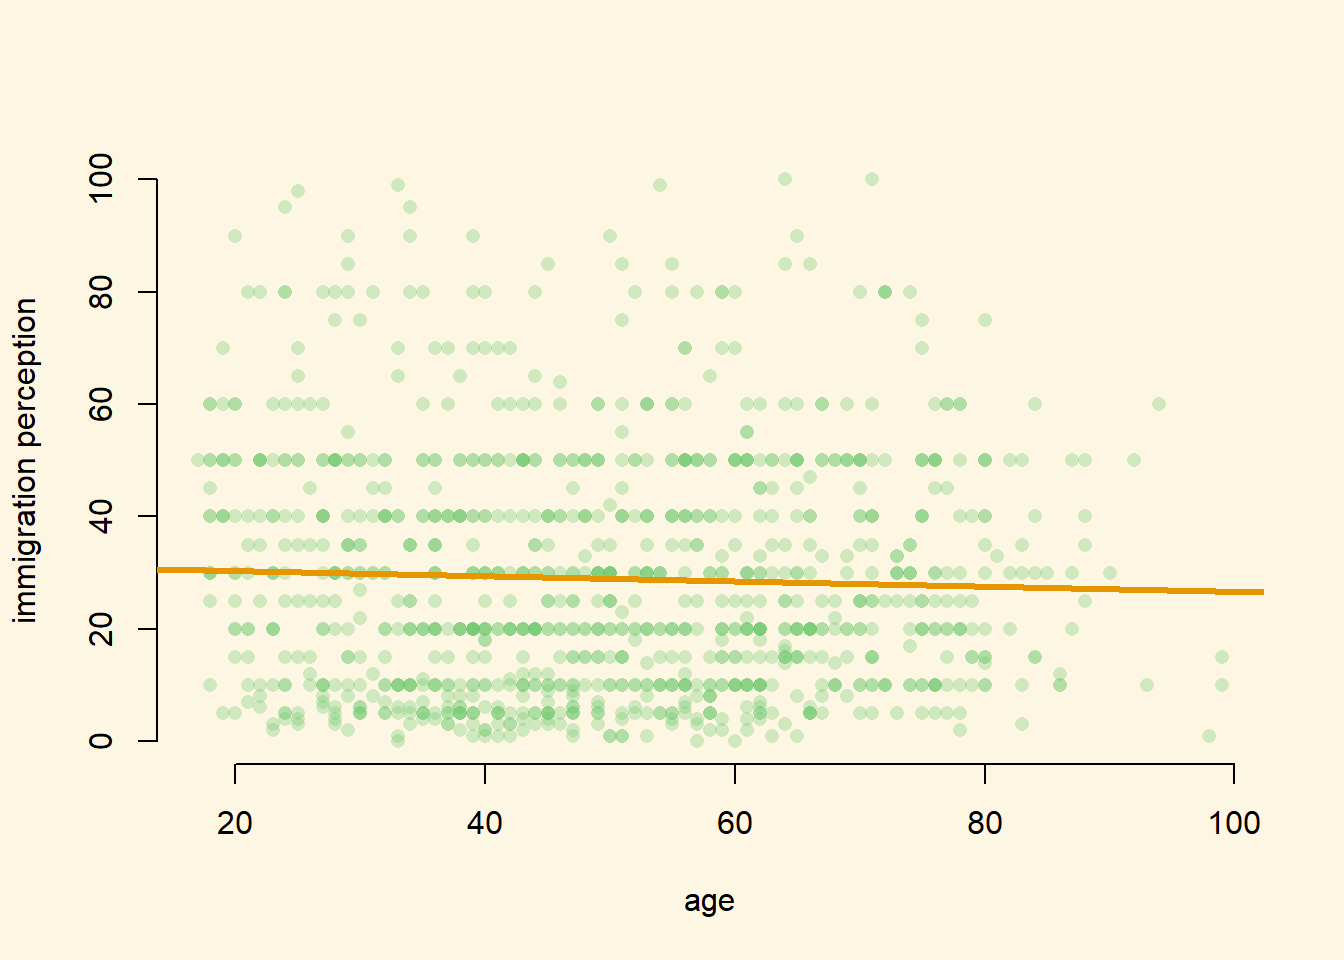
\includegraphics{statistics1_files/figure-latex/unnamed-chunk-305-1.pdf}

The regression line slopes downward, ever so slightly, pointing towards
a tiny negative relationship. The residuals seem to be extraordinarily
large. It seems, that the relation between age and immigration
perception is weak at best. This is more consistent with no
relationship.

\paragraph{Exercise 6}\label{exercise-6-5}

Interpret the regression output and try to imagine that you are
communicating your results to someone who does not know anything about
statistics.

\begin{Shaded}
\begin{Highlighting}[]
\KeywordTok{library}\NormalTok{(texreg)}
\KeywordTok{screenreg}\NormalTok{(m1)}
\end{Highlighting}
\end{Shaded}

\begin{verbatim}

========================
             Model 1    
------------------------
(Intercept)    31.38 ***
               (1.95)   
RAge           -0.05    
               (0.04)   
------------------------
R^2             0.00    
Adj. R^2        0.00    
Num. obs.    1049       
RMSE           21.06    
========================
*** p < 0.001, ** p < 0.01, * p < 0.05
\end{verbatim}

We cannot, with sufficient confidence, rule out that age and immigration
perception are unrelated (\(p > 0.05\)).

As we will learn next week, \(R^2\) indicates, that our model does a
terrible job at predicting the perception of immigration. We could
predict the outcome (perception of immigration) equally well without our
model.

Suppose, our best guess of \texttt{IMMBRIT} for any age is just the mean
of \texttt{IMMBRIT}. The quality of that prediction (in statistics
jargon, the naive guess) would be as good as the predictions we get from
our model.

\paragraph{Exercise 7}\label{exercise-7-4}

Estimate another model (i.e.~choose a different independent variable) on
the same dependent variable. Justify the choice.

\begin{Shaded}
\begin{Highlighting}[]
\NormalTok{m2 <-}\StringTok{ }\KeywordTok{lm}\NormalTok{(IMMBRIT }\OperatorTok{~}\StringTok{ }\NormalTok{HHInc, }\DataTypeTok{data =}\NormalTok{ data2)}
\end{Highlighting}
\end{Shaded}

We choose income as the predictor in our second model. We conjecture
that on average, wealthier people are more educated and hence have a
more realistic view of immigration. Furthermore, they tend to face less
competition from immigration and, therefore, tend not to exaggerate the
level of immigration. We expect that the wealthier the respondent, the
lower the respondent's estimate of immigration.

\paragraph{Exercise 8}\label{exercise-8-5}

Interpret the new regression output.

\begin{Shaded}
\begin{Highlighting}[]
\KeywordTok{screenreg}\NormalTok{(m2)}
\end{Highlighting}
\end{Shaded}

\begin{verbatim}

========================
             Model 1    
------------------------
(Intercept)    43.12 ***
               (1.41)   
HHInc          -1.47 ***
               (0.13)   
------------------------
R^2             0.10    
Adj. R^2        0.10    
Num. obs.    1049       
RMSE           19.94    
========================
*** p < 0.001, ** p < 0.01, * p < 0.05
\end{verbatim}

In line with our expectation, wealthier people perceive immigration to
be lower than poorer people. The relationship is significant at the five
percent level. We explain a tenth of the variance in the perception of
immigration with our model (you will learn this next week). Considering
that this model is very small (we use only one predictor variable), we
do quite well at predicting the outcome.

\paragraph{Exercise 9}\label{exercise-9-4}

Compare the two models and explain which one you would choose.

\begin{Shaded}
\begin{Highlighting}[]
\KeywordTok{screenreg}\NormalTok{( }\KeywordTok{list}\NormalTok{(m1, m2))}
\end{Highlighting}
\end{Shaded}

\begin{verbatim}

=====================================
             Model 1      Model 2    
-------------------------------------
(Intercept)    31.38 ***    43.12 ***
               (1.95)       (1.41)   
RAge           -0.05                 
               (0.04)                
HHInc                       -1.47 ***
                            (0.13)   
-------------------------------------
R^2             0.00         0.10    
Adj. R^2        0.00         0.10    
Num. obs.    1049         1049       
RMSE           21.06        19.94    
=====================================
*** p < 0.001, ** p < 0.01, * p < 0.05
\end{verbatim}

From what we have learned so far, we would look at the coefficients in
our models. In the first, Age was insignificant. In the second, income
is. Therefore, the second model is better at explaining perception on
immigration. We learn nothing about potential causes of overestimating
immigration from model one, whereas from model two, we do.

\paragraph{Exercise 10}\label{exercise-10-4}

\begin{Shaded}
\begin{Highlighting}[]
\KeywordTok{htmlreg}\NormalTok{( }\KeywordTok{list}\NormalTok{(m1, m2), }\DataTypeTok{file =} \StringTok{"regressions_on_immigration_perception.doc"}\NormalTok{)}
\end{Highlighting}
\end{Shaded}

\paragraph{Exercise 11}\label{exercise-11-3}

Consider the following table. This analysis asks whether individuals who
have spent longer in education have higher yearly earnings. The analysis
is based on a sample of 300 individuals. The dependent variable in this
analysis is the yearly income of the individual in UK pounds
(\texttt{earnings}). The independent variable measures the number of
years the individual spent in full-time education (\texttt{education}).

\begin{itemize}
\tightlist
\item
  Interpret the coefficient on the \texttt{education} variable.
\end{itemize}

For each additional year of education we expect earnings to go up by
1270.81 pounds on average.

\begin{itemize}
\tightlist
\item
  Using the values given in the table, calculate the test-statistic
\end{itemize}

We compute the t value using the formula:
\[ \frac{\bar{Y_{HA}}-\mu_{H_{0}}}{ \sigma_{\bar{Y_{HA}}} } \]

So, we take the alternative hypothesis (our estimate of the effect of
education) minus the mean under the null hypothesis and divide the
result by the standard error of our estimate. Unless stated otherwise,
the null hypothesis is that there is no effect of education on income,
i.e.~the null is zero.

The coefficient estimate here is \(1270.81\) and its standard error is
\(160.97\).

\begin{Shaded}
\begin{Highlighting}[]
\FloatTok{1270.81} \OperatorTok{/}\StringTok{ }\FloatTok{160.97}
\end{Highlighting}
\end{Shaded}

\begin{verbatim}
[1] 7.894701
\end{verbatim}

The t value is 7.89.

\begin{itemize}
\tightlist
\item
  Can we reject the null hypothesis of no effect at the 95\% confidence
  level? (Just looking at the stars is not sufficient here! How can we
  work out the result of the hypothesis test?)
\end{itemize}

We have 300 observations in our sample and because we estimate two
parameters, 298 degrees of freedom. A t distribution with 298 degrees of
freedom is well approximated by the standard normal distribution. Under
the normal distribution \(95\%\) are within \(1.96\) standard deviations
from the mean. Our t value is more extreme than that. Our estimate is
\(7.89\) standard deviations from the mean. It is unlikely to observe
such an extreme value by chance (assuming the null hypothesis, there is
no relation between education and income, is true). We therefore, reject
the null hypothesis at 5 percent level.

\section{Multiple linear regression models
(I)}\label{multiple-linear-regression-models-i}

\subsection{Seminar}\label{seminar-6}

\begin{Shaded}
\begin{Highlighting}[]
\KeywordTok{library}\NormalTok{(foreign) }
\KeywordTok{library}\NormalTok{(texreg)}
\end{Highlighting}
\end{Shaded}

\begin{Shaded}
\begin{Highlighting}[]
\KeywordTok{rm}\NormalTok{(}\DataTypeTok{list =} \KeywordTok{ls}\NormalTok{())}
\end{Highlighting}
\end{Shaded}

\subsubsection{Loading, Understanding and Cleaning our
Data}\label{loading-understanding-and-cleaning-our-data}

Today, we load the full standard (cross-sectional) dataset from the
Quality of Government Institute (this is a newer version that the one we
used in week 3). This is a great data source for comparativist political
science research. The codebook is available from their main
\href{http://qog.pol.gu.se/data/datadownloads/qogstandarddata}{website}.
You can also find time-series and cross-section data sets on this page.

The dataset is in stata format (\texttt{.dta}). Loading it requires the
\texttt{foreign} library and the \texttt{read.dta()} function which
operates similar to \texttt{read.csv()}.

Let's load the data set

\begin{Shaded}
\begin{Highlighting}[]
\CommentTok{# load dataset in Stata format from online source}
\NormalTok{world_data <-}\StringTok{ }\KeywordTok{read.dta}\NormalTok{(}\StringTok{"https://github.com/philippbroniecki/statistics1/raw/master/data/qog_std_cs_jan15.dta"}\NormalTok{)}

\CommentTok{# check the dimensions of the dataset}
\KeywordTok{dim}\NormalTok{(world_data)}
\end{Highlighting}
\end{Shaded}

\begin{verbatim}
[1]  193 2037
\end{verbatim}

The dataset contains many variables. We will select a subset of
variables that we want to work with. We are interested in political
stability. Specifically, we want to find out what predicts the level of
political stability. Therefore, \texttt{political\_stability} is our
dependent variable (also called response variable, left-hand-side
variable, explained/predicted variable). We will also select a variable
that identifies each row (observation) in the dataset uniquely:
\texttt{cname} which is the name of the country. Potential predictors
(independent variables, right-hand-side variables, covariates) are:

\begin{enumerate}
\def\labelenumi{\arabic{enumi}.}
\tightlist
\item
  \texttt{lp\_lat\_abst} is the distance to the equator which we rename
  into \texttt{latitude}
\item
  \texttt{dr\_ing} is an index for the level of globalization which we
  rename to \texttt{globalization}
\item
  \texttt{ti\_cpi} is Transparency International's Corruptions
  Perceptions Index, renamed to \texttt{institutions\_quality} (larger
  values mean better quality institutions, i.e.~less corruption)
\item
  \texttt{br\_dem} is a factor variable stating whether the relevant
  country is a democracy or not (with labels \texttt{"1.\ Democracy"}
  and \texttt{"0.\ Dictatorship"})
\end{enumerate}

Our dependent variable:

\begin{itemize}
\tightlist
\item
  \texttt{wbgi\_pse} which we rename into \texttt{political\_stability}
  (larger values mean more stability)
\end{itemize}

One approach of selecting a subset of variables we're interested in, is
to use the square bracket
\href{http://bit.ly/R_extract}{\texttt{{[}\ {]}} operator}. But first,
we rename the variables we care about like we did last week.

\begin{Shaded}
\begin{Highlighting}[]
\KeywordTok{names}\NormalTok{(world_data)[}\KeywordTok{which}\NormalTok{(}\KeywordTok{names}\NormalTok{(world_data) }\OperatorTok{==}\StringTok{ "cname"}\NormalTok{)] <-}\StringTok{ "country"}
\KeywordTok{names}\NormalTok{(world_data)[}\KeywordTok{which}\NormalTok{(}\KeywordTok{names}\NormalTok{(world_data) }\OperatorTok{==}\StringTok{ "wbgi_pse"}\NormalTok{)] <-}\StringTok{ "political_stability"}
\KeywordTok{names}\NormalTok{(world_data)[}\KeywordTok{which}\NormalTok{(}\KeywordTok{names}\NormalTok{(world_data) }\OperatorTok{==}\StringTok{ "lp_lat_abst"}\NormalTok{)] <-}\StringTok{ "latitude"}
\KeywordTok{names}\NormalTok{(world_data)[}\KeywordTok{which}\NormalTok{(}\KeywordTok{names}\NormalTok{(world_data) }\OperatorTok{==}\StringTok{ "dr_ig"}\NormalTok{)] <-}\StringTok{ "globalization"}
\KeywordTok{names}\NormalTok{(world_data)[}\KeywordTok{which}\NormalTok{(}\KeywordTok{names}\NormalTok{(world_data) }\OperatorTok{==}\StringTok{ "chga_demo"}\NormalTok{)] <-}\StringTok{ "democracy"}
\KeywordTok{names}\NormalTok{(world_data)[}\KeywordTok{which}\NormalTok{(}\KeywordTok{names}\NormalTok{(world_data) }\OperatorTok{==}\StringTok{ "ti_cpi"}\NormalTok{)] <-}\StringTok{ "institutions_quality"}
\end{Highlighting}
\end{Shaded}

Now, we take our subset. We will create an object named \texttt{keep}
which is a vector of the variable names that we would like to keep for
the analysis. We can then use this vector to subset our
\texttt{world\_data} object by including it within the square
parentheses:

\begin{Shaded}
\begin{Highlighting}[]
\NormalTok{keep <-}\StringTok{ }\KeywordTok{c}\NormalTok{(}\StringTok{"country"}\NormalTok{, }\StringTok{"political_stability"}\NormalTok{, }\StringTok{"latitude"}\NormalTok{, }\StringTok{"globalization"}\NormalTok{,}\StringTok{"democracy"}\NormalTok{, }\StringTok{"institutions_quality"}\NormalTok{)}
\NormalTok{world_data <-}\StringTok{ }\NormalTok{world_data[, keep]}
\end{Highlighting}
\end{Shaded}

Let's make sure we've got everything we need

\begin{Shaded}
\begin{Highlighting}[]
\KeywordTok{head}\NormalTok{(world_data)}
\end{Highlighting}
\end{Shaded}

\begin{verbatim}
              country political_stability  latitude globalization
1         Afghanistan          -2.5498192 0.3666667      31.46042
2             Albania          -0.1913142 0.4555556      58.32265
3             Algeria          -1.2624909 0.3111111      52.37114
4             Andorra           1.3064846 0.4700000            NA
5              Angola          -0.2163249 0.1366667      44.73296
6 Antigua and Barbuda           0.9319394 0.1892222      48.15911
        democracy institutions_quality
1 0. Dictatorship                  1.4
2    1. Democracy                  3.3
3 0. Dictatorship                  2.9
4    1. Democracy                   NA
5 0. Dictatorship                  1.9
6    1. Democracy                   NA
\end{verbatim}

The function \texttt{summary()} lets you summarize data sets. We will
look at the dataset now. When the dataset is small in the sense that you
have few variables (columns) then this is a very good way to get a good
overview. It gives you an idea about the level of measurement of the
variables and the scale. \texttt{country}, for example, is a character
variable as opposed to a number. Countries do not have any order, so the
level of measurement is categorical.

If you think about the next variable, political stability, and how one
could measure it you know there is an order implicit in the measurement:
more or less stability. From there, what you need to know is whether the
more or less is ordinal or interval scaled. Checking
\texttt{political\_stability} you see a range from roughly -3 to 1.5.
The variable is numerical and has decimal places. This tells you that
the variable is at least interval scaled. You will not see ordinally
scaled variables with decimal places. Examine the summaries of the other
variables and determine their level of measurement.

\begin{Shaded}
\begin{Highlighting}[]
\KeywordTok{summary}\NormalTok{(world_data)}
\end{Highlighting}
\end{Shaded}

\begin{verbatim}
   country          political_stability    latitude      globalization  
 Length:193         Min.   :-3.10637    Min.   :0.0000   Min.   :24.35  
 Class :character   1st Qu.:-0.72686    1st Qu.:0.1444   1st Qu.:45.22  
 Mode  :character   Median :-0.01900    Median :0.2444   Median :54.99  
                    Mean   :-0.06079    Mean   :0.2865   Mean   :57.15  
                    3rd Qu.: 0.78486    3rd Qu.:0.4444   3rd Qu.:68.34  
                    Max.   : 1.57240    Max.   :0.7222   Max.   :92.30  
                                        NA's   :12       NA's   :12     
           democracy   institutions_quality
 0. Dictatorship: 74   Min.   :1.010       
 1. Democracy   :118   1st Qu.:2.400       
 NA's           :  1   Median :3.300       
                       Mean   :3.988       
                       3rd Qu.:5.100       
                       Max.   :9.300       
                       NA's   :12          
\end{verbatim}

The variables \texttt{latitude}, \texttt{globalization} and
\texttt{inst\_quality} have 12 missing values each marked as
\texttt{NA}. \texttt{democracy} has 1 missing value. Missing values
could cause trouble because operations including an \texttt{NA} will
produce \texttt{NA} as a result (e.g.: \texttt{1\ +\ NA\ =\ NA}). We
will drop these missing values from our data set using the
\texttt{is.na()} function and square brackets. The exlamation mark in
front of \texttt{is.na()} means ``not''. So, we keep all rows that are
not NA's on the variable \texttt{latitude}.

\begin{Shaded}
\begin{Highlighting}[]
\NormalTok{world_data <-}\StringTok{ }\NormalTok{world_data[ }\OperatorTok{!}\KeywordTok{is.na}\NormalTok{(world_data}\OperatorTok{$}\NormalTok{latitude) ,]}
\end{Highlighting}
\end{Shaded}

Generally, we want to make sure we drop missing values only from
variables that we care about. Now that you have seen how to do this,
drop missings from \texttt{globalization},
\texttt{institutions\_quality}, and \texttt{democracy} yourself.

\begin{Shaded}
\begin{Highlighting}[]
\NormalTok{world_data <-}\StringTok{ }\NormalTok{world_data[ }\OperatorTok{!}\KeywordTok{is.na}\NormalTok{(world_data}\OperatorTok{$}\NormalTok{globalization) ,]}
\NormalTok{world_data <-}\StringTok{ }\NormalTok{world_data[ }\OperatorTok{!}\KeywordTok{is.na}\NormalTok{(world_data}\OperatorTok{$}\NormalTok{institutions_quality) ,]}
\NormalTok{world_data <-}\StringTok{ }\NormalTok{world_data[ }\OperatorTok{!}\KeywordTok{is.na}\NormalTok{(world_data}\OperatorTok{$}\NormalTok{democracy) ,]}
\end{Highlighting}
\end{Shaded}

\begin{Shaded}
\begin{Highlighting}[]
\KeywordTok{summary}\NormalTok{(world_data)}
\end{Highlighting}
\end{Shaded}

\begin{verbatim}
   country          political_stability    latitude      globalization  
 Length:170         Min.   :-2.67338    Min.   :0.0000   Min.   :25.46  
 Class :character   1st Qu.:-0.79223    1st Qu.:0.1386   1st Qu.:46.05  
 Mode  :character   Median :-0.03174    Median :0.2500   Median :55.87  
                    Mean   :-0.12018    Mean   :0.2865   Mean   :57.93  
                    3rd Qu.: 0.66968    3rd Qu.:0.4444   3rd Qu.:69.02  
                    Max.   : 1.48047    Max.   :0.7222   Max.   :92.30  
           democracy   institutions_quality
 0. Dictatorship: 67   Min.   :1.400       
 1. Democracy   :103   1st Qu.:2.500       
                       Median :3.300       
                       Mean   :4.050       
                       3rd Qu.:5.175       
                       Max.   :9.300       
\end{verbatim}

Let's look at the output of \texttt{summary(world\_data)} again and
check the range of the variable \texttt{latitude}. It is between
\texttt{0} and \texttt{1}. The codebook clarifies that the latitude of a
country's capital has been divided by \texttt{90} to get a variable that
ranges from \texttt{0} to \texttt{1}. This would make interpretation
difficult. When interpreting the effect of such a variable a unit change
(a change of \texttt{1}) covers the entire range or put differently, it
is a change from a country at the equator to a country at one of the
poles.

We therefore multiply by \texttt{90} again. This will turn the units of
the \texttt{latitude} variable into degrees again which makes
interpretation easier.

\begin{Shaded}
\begin{Highlighting}[]
\CommentTok{# transform latitude variable}
\NormalTok{world_data}\OperatorTok{$}\NormalTok{latitude <-}\StringTok{ }\NormalTok{world_data}\OperatorTok{$}\NormalTok{latitude }\OperatorTok{*}\StringTok{ }\DecValTok{90}
\end{Highlighting}
\end{Shaded}

\subsubsection{Estimating a Bivariate
Regression}\label{estimating-a-bivariate-regression}

Is there a correlation between the distance of a country to the equator
and the level of political stability? Both political stability
(dependent variable) and distance to the equator (independent variable)
are continuous. Therefore, we will get an idea about the relationship
using a scatter plot.

\begin{Shaded}
\begin{Highlighting}[]
\KeywordTok{plot}\NormalTok{(political_stability }\OperatorTok{~}\StringTok{ }\NormalTok{latitude, }\DataTypeTok{data =}\NormalTok{ world_data)}
\end{Highlighting}
\end{Shaded}

\includegraphics{statistics1_files/figure-latex/unnamed-chunk-325-1.pdf}

Looking at the cloud of points suggests that there might be a positive
relationship: increases in our independent variable \texttt{latitude}
appear to be associated with increases in the dependent variable
\texttt{political\_stability} (the further from the equator, the more
stable).

We can fit a line of best fit through the points. To do this we must
estimate the bivariate regression model with the \texttt{lm()} function
and then plot the line using the \texttt{abline()} function.

\begin{Shaded}
\begin{Highlighting}[]
\NormalTok{latitude_model <-}\StringTok{ }\KeywordTok{lm}\NormalTok{(political_stability }\OperatorTok{~}\StringTok{ }\NormalTok{latitude, }\DataTypeTok{data =}\NormalTok{ world_data)}

\CommentTok{# add the line}
\KeywordTok{plot}\NormalTok{(political_stability }\OperatorTok{~}\StringTok{ }\NormalTok{latitude, }\DataTypeTok{data =}\NormalTok{ world_data)}
\KeywordTok{abline}\NormalTok{(latitude_model)}
\end{Highlighting}
\end{Shaded}

\includegraphics{statistics1_files/figure-latex/unnamed-chunk-326-1.pdf}

We can also view a simple summary of the regression by using the
\texttt{screenreg} function:

\begin{Shaded}
\begin{Highlighting}[]
\CommentTok{# regression output}
\KeywordTok{screenreg}\NormalTok{(latitude_model)}
\end{Highlighting}
\end{Shaded}

\begin{verbatim}

=======================
             Model 1   
-----------------------
(Intercept)   -0.58 ***
              (0.12)   
latitude       0.02 ***
              (0.00)   
-----------------------
R^2            0.11    
Adj. R^2       0.10    
Num. obs.    170       
RMSE           0.89    
=======================
*** p < 0.001, ** p < 0.01, * p < 0.05
\end{verbatim}

Thinking back to last week, how can we interpret this regression ouput?

\begin{itemize}
\tightlist
\item
  The coefficient for the variable \texttt{latitude} (\(\beta_1\))
  indicates that a one-unit increase in a country's latitude is
  associated with a \texttt{0.02} increase in the measure of political
  stability, on average. Question: Is this association statistically
  significant at the 95\% confidence level?
\item
  The coefficient for the \texttt{(intercept)} term (\(\beta_0\))
  indicates that the average level of political stability for a country
  with a latitude of 0 is \(-0.58\) (where \texttt{latitude\ =\ 0} is a
  country positioned at the equator)
\item
  The \(R^2\) of the model is 0.11. This implies that 11\% of the
  variation in the dependent variable (political stability) is explained
  by the independent variable (latitude) in the model.
\end{itemize}

\subsubsection{Multivariate Regression}\label{multivariate-regression}

The regression above suggests that there is a significant association
between these variables However, as good social scientistis, we probably
do not think that the distance of a country from the equator is a
theoretically relevant variable for explaining political stability. This
is because there is no plausible causal link between the two. We should
therefore consider other variables to include in our model.

We will include the index of globalization (higher values mean more
integration with the rest of the world), the quality of institutions,
and the indicator for whether the country is a democracy. For all of
these variables we can come up with a theoretical story for their effect
on political stability.

To specify a \emph{multiple} linear regression model, the only thing we
need to change is what we pass to the \texttt{formula} argument of the
\texttt{lm()} function. In particular, if we wish to add additional
explanatory variables, the formula argument will take the following
form:

\begin{Shaded}
\begin{Highlighting}[]
\NormalTok{dependent.variable }\OperatorTok{~}\StringTok{ }\NormalTok{independent.variable.}\DecValTok{1} \OperatorTok{+}\StringTok{ }\NormalTok{independent.variable.}\DecValTok{2}\NormalTok{ ... independent.variable.k}
\end{Highlighting}
\end{Shaded}

where \texttt{k} indicates the total number of independent variables we
would like to include in the model. In the example here, our model would
therefore look like the following:

\begin{Shaded}
\begin{Highlighting}[]
\CommentTok{# model with more explanatory variables}
\NormalTok{inst_model <-}\StringTok{ }\KeywordTok{lm}\NormalTok{(political_stability }\OperatorTok{~}\StringTok{ }\NormalTok{latitude }\OperatorTok{+}\StringTok{ }\NormalTok{globalization }\OperatorTok{+}\StringTok{ }\NormalTok{institutions_quality }\OperatorTok{+}\StringTok{ }\NormalTok{democracy, }
                 \DataTypeTok{data =}\NormalTok{ world_data)}
\end{Highlighting}
\end{Shaded}

Remember, \texttt{political\_stability} is our dependent variable, as
before, and now we have four independent variables: \texttt{latitude},
\texttt{globalization}, \texttt{democracy} and
\texttt{institutions\_quality}. Again, just as with the bivariate model,
we can view the summarised output of the regression by using
\texttt{screenreg()}. As we now have two models (a simple regression
model, and a multiple regression model), we can join them together using
the \texttt{list()} function, and then put all of that inside
\texttt{screenreg()}.

\begin{Shaded}
\begin{Highlighting}[]
\KeywordTok{screenreg}\NormalTok{(}\KeywordTok{list}\NormalTok{(latitude_model, inst_model))}
\end{Highlighting}
\end{Shaded}

\begin{verbatim}

=============================================
                       Model 1     Model 2   
---------------------------------------------
(Intercept)             -0.58 ***   -1.25 ***
                        (0.12)      (0.20)   
latitude                 0.02 ***    0.00    
                        (0.00)      (0.00)   
globalization                       -0.00    
                                    (0.01)   
institutions_quality                 0.34 ***
                                    (0.04)   
democracy1. Democracy                0.04    
                                    (0.11)   
---------------------------------------------
R^2                      0.11        0.50    
Adj. R^2                 0.10        0.49    
Num. obs.              170         170       
RMSE                     0.89        0.67    
=============================================
*** p < 0.001, ** p < 0.01, * p < 0.05
\end{verbatim}

Including the two new predictors leads to substantial changes.

\begin{itemize}
\tightlist
\item
  First, we now explain 50\% of the variance of our dependent variable
  instead of just 11\%.
\item
  Second, the effect of the distance to the equator is no longer
  significant.
\item
  Third, better quality institutions are associated with more political
  stability. In particular, a one-unit increase in the measure of
  instituion quality (which ranges from 1 to 10) is associated with a
  0.34 increase in the measure for political stability.
\item
  Fourth, there is no significant relationship between globalization and
  political stability in this data.
\item
  Fifth, there is no significant relationship between democracy and
  political stability in this data.
\end{itemize}

\subsubsection{Joint Significance Test
(F-statistic)}\label{joint-significance-test-f-statistic}

Whenever you add variables to your model, you will explain more of the
variance in the dependent variable. That means, using your data, your
model will better predict outcomes. We would like to know whether the
difference (the added explanatory power) is statistically significant.
The null hypothesis is that the added explanatory power is zero and the
p-value gives us the probability of observing such a difference as the
one we actually computed assuming that null hypothesis (no difference)
is true.

The F-test is a joint hypothesis test that lets us compute that p-value.
Two conditions must be fulfilled to run an F-test:

\begin{longtable}[]{@{}l@{}}
\toprule
\begin{minipage}[b]{0.96\columnwidth}\raggedright\strut
Conditions for F-test model comparison\strut
\end{minipage}\tabularnewline
\midrule
\endhead
\begin{minipage}[t]{0.96\columnwidth}\raggedright\strut
Both models must be estimated from the same sample! If your added
variables contain lots of missing values and therefore your \texttt{n}
(number of observations) are reduced substantially, you are not
estimating from the same sample.\strut
\end{minipage}\tabularnewline
\begin{minipage}[t]{0.96\columnwidth}\raggedright\strut
The models must be nested. That means, the model with more variables
must contain all of the variables that are also in the model with fewer
variables.\strut
\end{minipage}\tabularnewline
\bottomrule
\end{longtable}

We specify two models: a restricted model and an unrestricted model. The
restricted model is the one with fewer variables. The unrestricted model
is the one including the extra variables. We say restricted model
because we are ``restricting'' it to NOT depend on the extra variables.
Once we estimated those two models we compare the residual sum of
squares (RSS). The RSS is the sum over the squared deviations from the
regression line and that is the unexplained error. The restricted model
(fewer variables) is always expected to have a larger RSS than the
unrestricted model. Notice that this is same as saying: the restricted
model (fewer variables) has less explanatory power.

We test whether the reduction in the RSS is statistically significant
using a distribution called ``F distribution''. If it is, the added
variables are jointly (but not necessarily individually) significant.
You do not need to know how to calculate p-values from the F
distribution, as we can use the \texttt{anova()} function in R to do
this for us.

\begin{Shaded}
\begin{Highlighting}[]
\KeywordTok{anova}\NormalTok{(latitude_model, inst_model)}
\end{Highlighting}
\end{Shaded}

\begin{verbatim}
Analysis of Variance Table

Model 1: political_stability ~ latitude
Model 2: political_stability ~ latitude + globalization + institutions_quality + 
    democracy
  Res.Df     RSS Df Sum of Sq      F                Pr(>F)    
1    168 133.121                                              
2    165  74.229  3    58.892 43.636 < 0.00000000000000022 ***
---
Signif. codes:  0 '***' 0.001 '**' 0.01 '*' 0.05 '.' 0.1 ' ' 1
\end{verbatim}

As we can see from the output, the p-value here is \emph{very} small,
which means that we can reject the null hypothesis that the unrestricted
model has no more explanatory power than the restricted model.

\subsubsection{Predicting outcome conditional on institutional
quality}\label{predicting-outcome-conditional-on-institutional-quality}

Just as we did with the simple regression model last week, we can use
the fitted model object to calculate the fitted values of our dependent
variable for different values of our explanatory variables. To do so, we
again use the \texttt{predict()} function.

We proceed in three steps.

\begin{enumerate}
\def\labelenumi{\arabic{enumi}.}
\tightlist
\item
  We set the values of the covariates for which we would like to produce
  fitted values.

  \begin{itemize}
  \tightlist
  \item
    You will need to set covariate values for \emph{every} explanatory
    variable that you included in your model.
  \item
    As only one of our variables has a significant relationship with the
    outcome in the multiple regression model that we estimated above, we
    are really only interested in that variable
    (\texttt{institutions\_quality}).
  \item
    Therefore, we will calculate fitted values over the range of
    \texttt{institutions\_quality}, while setting the values of
    \texttt{latitude} and \texttt{globalization} to their mean values.
  \item
    As \texttt{democracy} is a factor variable, we cannot use the mean
    value. Instead, we will set \texttt{democracy} to be equal to
    \texttt{"1.\ Democracy"} which is the label for democratic countries
  \end{itemize}
\item
  We calculate the fitted values.
\item
  We report the results (here we will produce a plot).
\end{enumerate}

For step one, the following code produces a \texttt{data.frame} of new
covariate values for which we would like to calculate a fitted value
from our model:

\begin{Shaded}
\begin{Highlighting}[]
\NormalTok{## Set the values for the explanatory variables}
\NormalTok{data_for_fitted_values <-}\StringTok{ }\KeywordTok{data.frame}\NormalTok{(}\DataTypeTok{institutions_quality =} \KeywordTok{seq}\NormalTok{(}\DataTypeTok{from =} \FloatTok{1.4}\NormalTok{, }\DataTypeTok{to =} \FloatTok{9.3}\NormalTok{, }\DataTypeTok{by =} \DecValTok{1}\NormalTok{),}
                                     \DataTypeTok{globalization =} \KeywordTok{mean}\NormalTok{(world_data}\OperatorTok{$}\NormalTok{globalization),}
                                     \DataTypeTok{latitude =} \KeywordTok{mean}\NormalTok{(world_data}\OperatorTok{$}\NormalTok{latitude),}
                                     \DataTypeTok{democracy =} \StringTok{"1. Democracy"}
\NormalTok{                                     )}
\end{Highlighting}
\end{Shaded}

Here, we have set the \texttt{institutions\_quality} variable to vary
between 1.4 and 9.3, with increments of 1 unit. We have set
\texttt{globalization} to be equal to the mean value of
\texttt{globalization} in the \texttt{world\_data} object, and
\texttt{latitude} to be equal to the mean value of \texttt{latitude} in
the \texttt{world\_data} object. Finally, we have set \texttt{democracy}
to be equal to \texttt{"1.\ Democracy"} (the value for democratic
countries). We have then put all of these values into a new
\texttt{data.frame} called \texttt{data\_for\_fitted\_values} which we
will pass to the \texttt{predict()} function.

Before we do that, let's just take a quick look at the
\texttt{data\_for\_fitted\_values} object:

\begin{Shaded}
\begin{Highlighting}[]
\KeywordTok{head}\NormalTok{(data_for_fitted_values)}
\end{Highlighting}
\end{Shaded}

\begin{verbatim}
  institutions_quality globalization latitude    democracy
1                  1.4      57.93053 25.78218 1. Democracy
2                  2.4      57.93053 25.78218 1. Democracy
3                  3.4      57.93053 25.78218 1. Democracy
4                  4.4      57.93053 25.78218 1. Democracy
5                  5.4      57.93053 25.78218 1. Democracy
6                  6.4      57.93053 25.78218 1. Democracy
\end{verbatim}

As you can see, this has produced a data.frame in which every
observation has a different value of \texttt{institutions\_quality} but
the same value for \texttt{latitude}, \texttt{globalization}, and
\texttt{democracy}.

We can now calculate the fitted values for each of these combinations of
our explanatory variables by passing the
\texttt{data\_for\_fitted\_values} object to the \texttt{newdata}
argument of the \texttt{predict()} function.

\begin{Shaded}
\begin{Highlighting}[]
\CommentTok{# Calculate the fitted values}
\NormalTok{fitted_values <-}\StringTok{ }\KeywordTok{predict}\NormalTok{(inst_model, }\DataTypeTok{newdata =}\NormalTok{ data_for_fitted_values)}

\NormalTok{## Save the fitted values as a new variable in the data_for_fitted_values object}

\NormalTok{data_for_fitted_values}\OperatorTok{$}\NormalTok{fitted_values <-}\StringTok{ }\NormalTok{fitted_values}
\end{Highlighting}
\end{Shaded}

We can now look again at the \texttt{data\_for\_fitted\_values} object:

\begin{Shaded}
\begin{Highlighting}[]
\KeywordTok{head}\NormalTok{(data_for_fitted_values)}
\end{Highlighting}
\end{Shaded}

\begin{verbatim}
  institutions_quality globalization latitude    democracy fitted_values
1                  1.4      57.93053 25.78218 1. Democracy   -1.00319887
2                  2.4      57.93053 25.78218 1. Democracy   -0.66431685
3                  3.4      57.93053 25.78218 1. Democracy   -0.32543483
4                  4.4      57.93053 25.78218 1. Democracy    0.01344719
5                  5.4      57.93053 25.78218 1. Democracy    0.35232921
6                  6.4      57.93053 25.78218 1. Democracy    0.69121123
\end{verbatim}

Hey presto! Now, for each of our explanatory variable combinations, we
have the corresponding fitted values as calculated from our estimated
regression.

Finally, we can plot these values:

\begin{Shaded}
\begin{Highlighting}[]
\KeywordTok{plot}\NormalTok{(}
\NormalTok{  fitted_values }\OperatorTok{~}\StringTok{ }\NormalTok{institutions_quality, }\CommentTok{# Specify the formula for the plot (dependent.variable ~ independent.variable)}
  \DataTypeTok{data =}\NormalTok{ data_for_fitted_values, }\CommentTok{# Specify the data to use for the plot}
  \DataTypeTok{xlab =} \StringTok{"Institution Quality"}\NormalTok{, }\CommentTok{# Specify the X-axis title}
  \DataTypeTok{ylab =} \StringTok{"Fitted value for political stability"}\NormalTok{, }\CommentTok{# Specify the Y-axis title}
  \DataTypeTok{frame.plot =} \OtherTok{FALSE}\NormalTok{, }\CommentTok{# The frame.plot = FALSE argument removes the box from around the plot}
  \DataTypeTok{col =} \StringTok{"blue"}\NormalTok{, }\CommentTok{# The col argument specifies the color}
  \DataTypeTok{type =} \StringTok{"l"}\NormalTok{, }\CommentTok{# type = "l" will produce a line plot, rather than the default scatter plot}
  \DataTypeTok{lwd =} \DecValTok{3} \CommentTok{# lwd = 3 will increase the thinkness of the line on the plot}
\NormalTok{)}
\end{Highlighting}
\end{Shaded}

\includegraphics{statistics1_files/figure-latex/unnamed-chunk-336-1.pdf}

We could also use the output from our model to plot two separate lines
of fitted values: one for democracies, and one for dictatorships. We
have already done this for democracies, so the following code constructs
a \texttt{data.frame} of fitted values for dictatorships:

\begin{Shaded}
\begin{Highlighting}[]
\NormalTok{## Set the values for the explanatory variables}
\NormalTok{data_for_fitted_values_dictator <-}\StringTok{ }\KeywordTok{data.frame}\NormalTok{(}\DataTypeTok{institutions_quality =} \KeywordTok{seq}\NormalTok{(}\DataTypeTok{from =} \FloatTok{1.4}\NormalTok{, }\DataTypeTok{to =} \FloatTok{9.3}\NormalTok{, }\DataTypeTok{by =} \DecValTok{1}\NormalTok{),}
                                     \DataTypeTok{globalization =} \KeywordTok{mean}\NormalTok{(world_data}\OperatorTok{$}\NormalTok{globalization),}
                                     \DataTypeTok{latitude =} \KeywordTok{mean}\NormalTok{(world_data}\OperatorTok{$}\NormalTok{latitude),}
                                     \DataTypeTok{democracy =} \StringTok{"0. Dictatorship"}
\NormalTok{                                     )}

\CommentTok{# Calculate the fitted values}
\NormalTok{fitted_values_dictator <-}\StringTok{ }\KeywordTok{predict}\NormalTok{(inst_model, }\DataTypeTok{newdata =}\NormalTok{ data_for_fitted_values_dictator)}

\NormalTok{## Save the fitted values as a new variable in the data_for_fitted_values object}

\NormalTok{data_for_fitted_values_dictator}\OperatorTok{$}\NormalTok{fitted_values <-}\StringTok{ }\NormalTok{fitted_values_dictator}

\NormalTok{## Take a look at the output}
\KeywordTok{head}\NormalTok{(data_for_fitted_values_dictator)}
\end{Highlighting}
\end{Shaded}

\begin{verbatim}
  institutions_quality globalization latitude       democracy
1                  1.4      57.93053 25.78218 0. Dictatorship
2                  2.4      57.93053 25.78218 0. Dictatorship
3                  3.4      57.93053 25.78218 0. Dictatorship
4                  4.4      57.93053 25.78218 0. Dictatorship
5                  5.4      57.93053 25.78218 0. Dictatorship
6                  6.4      57.93053 25.78218 0. Dictatorship
  fitted_values
1   -1.04148517
2   -0.70260315
3   -0.36372113
4   -0.02483911
5    0.31404291
6    0.65292493
\end{verbatim}

Now that we have calculated these fitted values, we can add the line for
dictatorships to the plot we created above using the \texttt{lines()}
function:

\begin{Shaded}
\begin{Highlighting}[]
\NormalTok{## Create the same plot as above for fitted values over the range of institution quality for democracies}
\KeywordTok{plot}\NormalTok{(}
\NormalTok{  fitted_values }\OperatorTok{~}\StringTok{ }\NormalTok{institutions_quality, }\CommentTok{# Specify the formula for the plot (dependent.variable ~ independent.variable)}
  \DataTypeTok{data =}\NormalTok{ data_for_fitted_values, }\CommentTok{# Specify the data to use for the plot}
  \DataTypeTok{xlab =} \StringTok{"Institution Quality"}\NormalTok{, }\CommentTok{# Specify the X-axis title}
  \DataTypeTok{ylab =} \StringTok{"Fitted value for political stability"}\NormalTok{, }\CommentTok{# Specify the Y-axis title}
  \DataTypeTok{frame.plot =} \OtherTok{FALSE}\NormalTok{, }\CommentTok{# The frame.plot = FALSE argument removes the box from around the plot}
  \DataTypeTok{col =} \StringTok{"blue"}\NormalTok{, }\CommentTok{# The col argument specifies the color}
  \DataTypeTok{type =} \StringTok{"l"}\NormalTok{, }\CommentTok{# type = "l" will produce a line plot, rather than the default scatter plot}
  \DataTypeTok{lwd =} \DecValTok{3} \CommentTok{# lwd = 3 will increase the thinkness of the line on the plot}
\NormalTok{)}

\NormalTok{## Add an additional line of fitted values over the range of institution quality for dictatorships}
\KeywordTok{lines}\NormalTok{(}\DataTypeTok{x =}\NormalTok{ data_for_fitted_values_dictator}\OperatorTok{$}\NormalTok{institutions_quality, }
      \DataTypeTok{y =}\NormalTok{ data_for_fitted_values_dictator}\OperatorTok{$}\NormalTok{fitted_values,}
      \DataTypeTok{col =} \StringTok{"red"}\NormalTok{,}
      \DataTypeTok{lwd =} \DecValTok{3}\NormalTok{)}
\end{Highlighting}
\end{Shaded}

\includegraphics{statistics1_files/figure-latex/unnamed-chunk-338-1.pdf}

We can see from the plot that the fitted values for democracies (blue
line) are almost exactly the same as those for dictatorships (red line).
This is reassuring, as the estimated coefficient on the democracy
variable was very small (0.04) and was not statistically significantly
different from 0. Often, however, it can be very illuminating to
construct plots like this where we construct a line to indicate how our
predicted values for Y vary across one of our explanatory variables
(here, institution quality), and we create different lines for different
values of another explanatory variable (here, democracy/dictatorship).

\subsubsection{Additional Resources}\label{additional-resources-1}

Visualizing Distributions

\subsubsection{Exercises}\label{exercises-6}

\begin{enumerate}
\def\labelenumi{\arabic{enumi}.}
\tightlist
\item
  Open a new script and save it as assignment5.
\item
  Go to the
  \href{http://qog.pol.gu.se/data/datadownloads/qogstandarddata}{QoG
  website} and download the standard data and the accompanying codebook.
\item
  Pretend that you are writing a research paper. Select one dependent
  variable that you want to explain with a statistical model.
\item
  Run a simple regression (with one explanatory variable) on that
  dependent variable and justify your choice of explanatory variable.
  This will require you to think about the outcome that you are trying
  to explain, and what you think will be a good predictor for that
  outcome.
\item
  Add some additional explanatory variables (no more than 5) to your
  model and justify the choice again.
\item
  Carry out the F-test to check whether the new model explains more than
  the old model.
\item
  Produce a regression table of the better model.
\item
  Interpret the output of the better model. State your expectations and
  whether they were met.
\item
  Calculate fitted values whilst varying at least one of your continuous
  explanatory variables.
\item
  Plot the result.
\item
  Interpret the plot.
\item
  Source your entire script. If it produces errors, clean your script.
\end{enumerate}

\subsubsection{Midterm Preparation}\label{midterm-preparation}

We wrote a midterm preparation exercise for you. It envolves working a
little bit with data (in section 3). You will obviously not get
questions where you work with R, so you can skip that part of section 3
if you want.

Midterm Preparatory Questions Prepartory Questions Dataset Midterm
Preparatory Response

\subsection{Solutions}\label{solutions-6}

\begin{Shaded}
\begin{Highlighting}[]
\KeywordTok{library}\NormalTok{(texreg)}
\end{Highlighting}
\end{Shaded}

\paragraph{Exercise 2}\label{exercise-2-4}

You can download the data and load from your local disk but since it is
available online, we download it directly from the Quality of Government
Institute website.

\begin{Shaded}
\begin{Highlighting}[]
\NormalTok{df <-}\StringTok{ }\KeywordTok{read.csv}\NormalTok{(}\StringTok{"http://www.qogdata.pol.gu.se/data/qog_std_cs_jan17.csv"}\NormalTok{, }\DataTypeTok{header =} \OtherTok{TRUE}\NormalTok{)}
\end{Highlighting}
\end{Shaded}

\paragraph{Exercise 3}\label{exercise-3-6}

Pretend that you are writing a research paper. Select one dependent
variable that you want to explain with a statistical model.

We are interested in explaining the quality of government idicator,
where larger values indicate better overall governance. Before we go on
to check what predicts better governance, we will take a look at the
variable and remove NA's. We will also rename the variable.

\begin{Shaded}
\begin{Highlighting}[]
\CommentTok{# rename}
\KeywordTok{names}\NormalTok{(df)[}\KeywordTok{which}\NormalTok{(}\KeywordTok{names}\NormalTok{(df) }\OperatorTok{==}\StringTok{ "icrg_qog"}\NormalTok{)] <-}\StringTok{ "gov_quality"}

\CommentTok{# look at DV}
\KeywordTok{summary}\NormalTok{(df}\OperatorTok{$}\NormalTok{gov_quality) }\CommentTok{# 55 NA's}
\end{Highlighting}
\end{Shaded}

\begin{verbatim}
   Min. 1st Qu.  Median    Mean 3rd Qu.    Max.    NA's 
0.08333 0.38889 0.47222 0.52540 0.63194 0.97222      55 
\end{verbatim}

\begin{Shaded}
\begin{Highlighting}[]
\CommentTok{# create a copy of full dataset}
\NormalTok{df.full <-}\StringTok{ }\NormalTok{df}

\CommentTok{# drop NA's}
\NormalTok{df <-}\StringTok{ }\NormalTok{df[ }\OperatorTok{!}\KeywordTok{is.na}\NormalTok{(df}\OperatorTok{$}\NormalTok{gov_quality), ]}
\end{Highlighting}
\end{Shaded}

The range of the quality of government variable is 0 to 1. We will
re-scale to 0 - 100 to make results easier to interpret.

\begin{Shaded}
\begin{Highlighting}[]
\NormalTok{df}\OperatorTok{$}\NormalTok{gov_quality <-}\StringTok{ }\NormalTok{df}\OperatorTok{$}\NormalTok{gov_quality }\OperatorTok{*}\StringTok{ }\DecValTok{100}
\end{Highlighting}
\end{Shaded}

\paragraph{Exercise 4}\label{exercise-4-6}

From Putnam's ``bowling alone'', we know of the theory of the importance
of social capital for successful democratic governance. We, therefore,
choose the social capital indicator \texttt{bti\_sc}, where larger
values stand for more social capital. We expect better governance in
countries where social capital is higher. Before we estimate the model,
we look at the variable, remove missings, and rename it.

\begin{Shaded}
\begin{Highlighting}[]
\CommentTok{# look at IV}
\KeywordTok{summary}\NormalTok{(df}\OperatorTok{$}\NormalTok{bti_sc)}
\end{Highlighting}
\end{Shaded}

\begin{verbatim}
   Min. 1st Qu.  Median    Mean 3rd Qu.    Max.    NA's 
  1.000   4.000   5.000   5.324   6.000   9.000      34 
\end{verbatim}

\begin{Shaded}
\begin{Highlighting}[]
\CommentTok{# remove NA's}
\NormalTok{df <-}\StringTok{ }\NormalTok{df[ }\OperatorTok{!}\KeywordTok{is.na}\NormalTok{(df}\OperatorTok{$}\NormalTok{bti_sc), ]}

\CommentTok{# rename}
\KeywordTok{names}\NormalTok{(df)[}\KeywordTok{which}\NormalTok{(}\KeywordTok{names}\NormalTok{(df) }\OperatorTok{==}\StringTok{ "bti_sc"}\NormalTok{)] <-}\StringTok{ "social_capital"}
\end{Highlighting}
\end{Shaded}

Our sample size is down to 105 countries. This is still a decent sample
size. However, we would like to avoid loosing many more observations.
Smaller sample sizes are a danger to inference (through increased
variance - effects are less likely to be discovered and if they are,
they are more likely to be over-estimates).

\begin{Shaded}
\begin{Highlighting}[]
\CommentTok{# linear model}
\NormalTok{m1 <-}\StringTok{ }\KeywordTok{lm}\NormalTok{(gov_quality }\OperatorTok{~}\StringTok{ }\NormalTok{social_capital, }\DataTypeTok{data =}\NormalTok{ df)}
\KeywordTok{screenreg}\NormalTok{(m1)}
\end{Highlighting}
\end{Shaded}

\begin{verbatim}

==========================
                Model 1   
--------------------------
(Intercept)      24.68 ***
                 (4.02)   
social_capital    3.73 ***
                 (0.72)   
--------------------------
R^2               0.21    
Adj. R^2          0.20    
Num. obs.       105       
RMSE             12.41    
==========================
*** p < 0.001, ** p < 0.01, * p < 0.05
\end{verbatim}

Firstly, the intercept is not meaningful in this case because social
capital ranges from 1 to 9, i.e.~there is no country with 0 social
capital.

The coefficient of social capital is positive and significant. Dividing
the estimate by the standard error yields the t value which is 5.2. At a
conventional alpha level of 0.05, we reject the null hypothesis when t
is more extreme than \(\pm\) 1.96. This is the case here. In line with
our expectation, more social capital increases the quality of governance
on average by 3.73 points (on a 0 - 100 scale).

Increasing social capital by one point of its scale is a substantial
amount (1/9 or 11\(\%\) of its range). So, if social capital increases
by a substantial amount, does governance also go up by a substantial
amount? A 3.73 point change on a 0-100 scale is 3.73/101 or 4\(\%\).
That is still a substantial change considering that we are measuring how
well governed an entire country is.

\paragraph{Exercise 5}\label{exercise-5-6}

Add some additional explanatory variables (no more than 5) to your model
and justify the choice again.

We have not talked about this in the lecture before and it will not be a
hurdle in the midterm. However, it is important that you keep an eye on
sample size. If the sample size becomes too small it is unlikely that
you can make meaningful statements about the world. We, therefore,
selected variables with an eye on the missing values and their
theoretical importance. If you see studies that are based on small
samples, be suspicious.

Firstly, we used infant mortality as a general indicator for development
in the sense that basic health can be provided. We expect that if health
conditions get worse than that should affect the capacity to govern
negatively because it points to a basic lack of resources. We include a
variable that measures conflict intensity. Violent conflict seriously,
impedes the ability to govern. Finally, we added an index for the
freedom of the press. The press is often considered to be the forth
column in a state (besides the legislative, executive, and judicial
branches). The function is to check the government. A role, that can be
best fulfilled by a free press. This will lead to a more accountable
government which we conjecture increases the quality of government.

We rename the variables and drop missing values on them.

Note: To make models comparable, they should be based on the same
sample. So, after we dropped missing values, we have to re-run our
bivariate model as well.

\begin{Shaded}
\begin{Highlighting}[]
\CommentTok{# renaming}
\KeywordTok{names}\NormalTok{(df)[}\KeywordTok{which}\NormalTok{(}\KeywordTok{names}\NormalTok{(df)}\OperatorTok{==}\StringTok{"wef_imort"}\NormalTok{)] <-}\StringTok{ "infant_mortality"}
\KeywordTok{names}\NormalTok{(df)[}\KeywordTok{which}\NormalTok{(}\KeywordTok{names}\NormalTok{(df)}\OperatorTok{==}\StringTok{"fh_fotpsc"}\NormalTok{)] <-}\StringTok{ "press_freedom"}
\KeywordTok{names}\NormalTok{(df)[}\KeywordTok{which}\NormalTok{(}\KeywordTok{names}\NormalTok{(df)}\OperatorTok{==}\StringTok{"bti_ci"}\NormalTok{)] <-}\StringTok{ "conflict_intensity"}

\KeywordTok{summary}\NormalTok{(df}\OperatorTok{$}\NormalTok{infant_mortality) }\CommentTok{# infant mortality}
\end{Highlighting}
\end{Shaded}

\begin{verbatim}
   Min. 1st Qu.  Median    Mean 3rd Qu.    Max.    NA's 
   2.00    9.30   17.30   27.73   42.80  119.20      12 
\end{verbatim}

\begin{Shaded}
\begin{Highlighting}[]
\KeywordTok{summary}\NormalTok{(df}\OperatorTok{$}\NormalTok{press_freedom) }\CommentTok{# freedom of the press index}
\end{Highlighting}
\end{Shaded}

\begin{verbatim}
   Min. 1st Qu.  Median    Mean 3rd Qu.    Max. 
  16.00   41.00   57.00   55.57   68.00   97.00 
\end{verbatim}

\begin{Shaded}
\begin{Highlighting}[]
\KeywordTok{summary}\NormalTok{(df}\OperatorTok{$}\NormalTok{conflict_intensity) }\CommentTok{# conflict intensity}
\end{Highlighting}
\end{Shaded}

\begin{verbatim}
   Min. 1st Qu.  Median    Mean 3rd Qu.    Max. 
  1.000   3.000   4.000   4.762   6.000  10.000 
\end{verbatim}

\begin{Shaded}
\begin{Highlighting}[]
\CommentTok{# drop missings}
\NormalTok{df <-}\StringTok{ }\NormalTok{df[ }\OperatorTok{!}\KeywordTok{is.na}\NormalTok{(df}\OperatorTok{$}\NormalTok{infant_mortality) ,]}

\CommentTok{# re-run model 1 with new sample and check differences}
\NormalTok{m1.rerun <-}\StringTok{ }\KeywordTok{lm}\NormalTok{(gov_quality }\OperatorTok{~}\StringTok{ }\NormalTok{social_capital, }\DataTypeTok{data =}\NormalTok{ df)}
\KeywordTok{screenreg}\NormalTok{( }\KeywordTok{list}\NormalTok{(m1, m1.rerun) )}
\end{Highlighting}
\end{Shaded}

\begin{verbatim}

=====================================
                Model 1     Model 2  
-------------------------------------
(Intercept)      24.68 ***  30.11 ***
                 (4.02)     (4.52)   
social_capital    3.73 ***   2.93 ***
                 (0.72)     (0.79)   
-------------------------------------
R^2               0.21       0.13    
Adj. R^2          0.20       0.12    
Num. obs.       105         93       
RMSE             12.41      12.03    
=====================================
*** p < 0.001, ** p < 0.01, * p < 0.05
\end{verbatim}

As you can see, the difference is not small. This is less than ideal.
R\^{}2 goes down by alot and the magnitude of social capital also
changes. There is not much you can do (without advanced stats) except
being transparent about the differences.

\begin{Shaded}
\begin{Highlighting}[]
\CommentTok{# add new control variables}
\NormalTok{m2 <-}\StringTok{ }\KeywordTok{lm}\NormalTok{(gov_quality }\OperatorTok{~}\StringTok{ }\NormalTok{social_capital }\OperatorTok{+}\StringTok{ }\NormalTok{infant_mortality }\OperatorTok{+}\StringTok{ }\NormalTok{press_freedom }\OperatorTok{+}\StringTok{ }\NormalTok{conflict_intensity, }\DataTypeTok{data =}\NormalTok{ df )}
\KeywordTok{screenreg}\NormalTok{(}\KeywordTok{list}\NormalTok{(m1.rerun, m2))}
\end{Highlighting}
\end{Shaded}

\begin{verbatim}

=========================================
                    Model 1    Model 2   
-----------------------------------------
(Intercept)         30.11 ***   64.29 ***
                    (4.52)     (12.74)   
social_capital       2.93 ***   -0.08    
                    (0.79)      (1.27)   
infant_mortality                -0.23 ***
                                (0.05)   
press_freedom                   -0.10    
                                (0.10)   
conflict_intensity              -1.29    
                                (0.66)   
-----------------------------------------
R^2                  0.13        0.39    
Adj. R^2             0.12        0.37    
Num. obs.           93          93       
RMSE                12.03       10.21    
=========================================
*** p < 0.001, ** p < 0.01, * p < 0.05
\end{verbatim}

\paragraph{Exercise 6}\label{exercise-6-6}

Carry out the F-test to check whether the new model explains more than
the old model.

\begin{Shaded}
\begin{Highlighting}[]
\CommentTok{# f-test}
\KeywordTok{anova}\NormalTok{(m1.rerun, m2) }
\end{Highlighting}
\end{Shaded}

\begin{verbatim}
Analysis of Variance Table

Model 1: gov_quality ~ social_capital
Model 2: gov_quality ~ social_capital + infant_mortality + press_freedom + 
    conflict_intensity
  Res.Df   RSS Df Sum of Sq    F       Pr(>F)    
1     91 13170                                   
2     88  9169  3    4000.9 12.8 0.0000005133 ***
---
Signif. codes:  0 '***' 0.001 '**' 0.01 '*' 0.05 '.' 0.1 ' ' 1
\end{verbatim}

As we saw by comparing R\^{}2, the bigger model explains a lot more
variance in the quality of government. The f-test shows that this
difference is not due to chance. The p value is smaller than 0.05,
hence, we reject the null that the small model and the larger model
really explain the same. Another way to put this is: the variables we
have added are jointly significant.

\paragraph{Exercise 7}\label{exercise-7-5}

Produce a regression table of the better model.

\begin{Shaded}
\begin{Highlighting}[]
\KeywordTok{htmlreg}\NormalTok{(m2, }\DataTypeTok{file =} \StringTok{"regression_quality_of_government.doc"}\NormalTok{)}
\end{Highlighting}
\end{Shaded}

\begin{verbatim}
The table was written to the file 'regression_quality_of_government.doc'.
\end{verbatim}

\paragraph{Exercise 8}\label{exercise-8-6}

Interpret the output of the better model. State your expectations and
whether they were met.

\begin{Shaded}
\begin{Highlighting}[]
\KeywordTok{screenreg}\NormalTok{( }\KeywordTok{list}\NormalTok{(m1.rerun, m2))}
\end{Highlighting}
\end{Shaded}

\begin{verbatim}

=========================================
                    Model 1    Model 2   
-----------------------------------------
(Intercept)         30.11 ***   64.29 ***
                    (4.52)     (12.74)   
social_capital       2.93 ***   -0.08    
                    (0.79)      (1.27)   
infant_mortality                -0.23 ***
                                (0.05)   
press_freedom                   -0.10    
                                (0.10)   
conflict_intensity              -1.29    
                                (0.66)   
-----------------------------------------
R^2                  0.13        0.39    
Adj. R^2             0.12        0.37    
Num. obs.           93          93       
RMSE                12.03       10.21    
=========================================
*** p < 0.001, ** p < 0.01, * p < 0.05
\end{verbatim}

Our re-run bivariate model explains 13\(\%\) of the variance of the
quality of government. This is not bad for a small model. By adding our
three variables, we increased explained variance to 40\(\%\) which is a
large increase. Our new model seems to explain quality of government
much better than the smaller model.

The intercept is not meaningful in either model. The coefficient of
social capital is no longer significant (its standard error is larger in
absolute terms than the coefficient estimate). We, therefore, do find
evidence for the effect of social capital when we control basic health,
press freedom, and conflict intensity also. Neither press freedom nor
conflict intensity reach conventional levels of significance (both
coefficients are less than 1.96 standard deviations away from zero). We
find that the worth the health conditions, the less well governed a
country will be. Infant mortality is measured in deaths/ 1000 live
births. If that proportion increases by 10, the government index
decreases by 2.3 which corresponds to roughly 2\(\%\) of its range.

\paragraph{Exercise 9}\label{exercise-9-5}

Calculate fitted values whilst varying at least one of your continuous
explanatory variables.

We only have one significant variable. It does not make sense to vary
insignificant variables because, we cannot reject the null that their
effect is zero. We vary infant mortality from minimum to maximum.

\begin{Shaded}
\begin{Highlighting}[]
\CommentTok{# see minimum and maximum of infant mortality}
\KeywordTok{summary}\NormalTok{(df}\OperatorTok{$}\NormalTok{infant_mortality)}
\end{Highlighting}
\end{Shaded}

\begin{verbatim}
   Min. 1st Qu.  Median    Mean 3rd Qu.    Max. 
   2.00    9.30   17.30   27.73   42.80  119.20 
\end{verbatim}

\begin{Shaded}
\begin{Highlighting}[]
\CommentTok{# set our covariates}
\NormalTok{covariates <-}\StringTok{ }\KeywordTok{data.frame}\NormalTok{(}
  \DataTypeTok{social_capital =} \KeywordTok{mean}\NormalTok{(df}\OperatorTok{$}\NormalTok{social_capital), }
  \DataTypeTok{infant_mortality =} \KeywordTok{seq}\NormalTok{(}\DataTypeTok{from =} \DecValTok{2}\NormalTok{, }\DataTypeTok{to =} \DecValTok{120}\NormalTok{, }\DataTypeTok{by =} \DecValTok{1}\NormalTok{),}
  \DataTypeTok{press_freedom =} \KeywordTok{mean}\NormalTok{(df}\OperatorTok{$}\NormalTok{press_freedom),}
  \DataTypeTok{conflict_intensity =} \KeywordTok{mean}\NormalTok{(df}\OperatorTok{$}\NormalTok{conflict_intensity)}
\NormalTok{  )}

\CommentTok{# check that everything looks okay}
\KeywordTok{head}\NormalTok{(covariates) }\CommentTok{# looks fine}
\end{Highlighting}
\end{Shaded}

\begin{verbatim}
  social_capital infant_mortality press_freedom conflict_intensity
1       5.473118                2      53.92473           4.612903
2       5.473118                3      53.92473           4.612903
3       5.473118                4      53.92473           4.612903
4       5.473118                5      53.92473           4.612903
5       5.473118                6      53.92473           4.612903
6       5.473118                7      53.92473           4.612903
\end{verbatim}

\begin{Shaded}
\begin{Highlighting}[]
\CommentTok{# calculate fitted values using predict()}
\NormalTok{fitted.vals <-}\StringTok{ }\KeywordTok{predict}\NormalTok{(m2, }\DataTypeTok{newdata =}\NormalTok{ covariates)}

\CommentTok{# attch the fitted values to our covariates data}
\NormalTok{covariates}\OperatorTok{$}\NormalTok{fitted.vals <-}\StringTok{ }\NormalTok{fitted.vals}

\CommentTok{# hooray, for each scenario a predicted outcome}
\KeywordTok{head}\NormalTok{(covariates)}
\end{Highlighting}
\end{Shaded}

\begin{verbatim}
  social_capital infant_mortality press_freedom conflict_intensity
1       5.473118                2      53.92473           4.612903
2       5.473118                3      53.92473           4.612903
3       5.473118                4      53.92473           4.612903
4       5.473118                5      53.92473           4.612903
5       5.473118                6      53.92473           4.612903
6       5.473118                7      53.92473           4.612903
  fitted.vals
1    52.19227
2    51.95759
3    51.72292
4    51.48825
5    51.25358
6    51.01891
\end{verbatim}

\paragraph{Exercise 10}\label{exercise-10-5}

Plot the result.

\begin{Shaded}
\begin{Highlighting}[]
\KeywordTok{plot}\NormalTok{(}
  \DataTypeTok{y =}\NormalTok{ covariates}\OperatorTok{$}\NormalTok{fitted.vals,}
  \DataTypeTok{x =}\NormalTok{ covariates}\OperatorTok{$}\NormalTok{infant_mortality, }
  \DataTypeTok{frame.plot =} \OtherTok{FALSE}\NormalTok{,}
  \DataTypeTok{main =} \StringTok{"Effect of infant mortality on quality of government"}\NormalTok{,}
  \DataTypeTok{ylab =} \StringTok{"quality of government"}\NormalTok{,}
  \DataTypeTok{xlab =} \StringTok{"infant mortality per 100 live births"}\NormalTok{,}
  \DataTypeTok{type =} \StringTok{"l"}\NormalTok{,}
  \DataTypeTok{lwd =} \DecValTok{2}
\NormalTok{)}
\end{Highlighting}
\end{Shaded}

\includegraphics{statistics1_files/figure-latex/unnamed-chunk-353-1.pdf}

\paragraph{Exercise 11}\label{exercise-11-4}

Interpret the plot.

We interpret the simple plot including just the rgression line. It
illustrates the strong negative relation between infant mortality, our
proxy for basic health and resource conditions, and the quality of
government generally. At 20 deaths per 1000 live births, we predict
quality of government at roughly 48. At 100 deaths per 1000 live births,
quality of government is predicted to be at roughly 33 only. Therefore,
quality of government decreased by 31\(\%\) (\(\frac{48-33}{48}\)), a
substantial amount.

\paragraph{Extra Info (not relevant for
midterm)}\label{extra-info-not-relevant-for-midterm}

Below, we will show you how you could illustrate the confidence interval
around the prediction. This is not necessary for the midterm but usefule
to know. We can set the option \texttt{se.fit\ =\ TRUE} which will
return standard errors for the prediction as well.

\begin{Shaded}
\begin{Highlighting}[]
\NormalTok{prediction.with.se <-}\StringTok{ }\KeywordTok{predict}\NormalTok{(m2, }\DataTypeTok{newdata =}\NormalTok{ covariates, }\DataTypeTok{se.fit =} \OtherTok{TRUE}\NormalTok{)}
\end{Highlighting}
\end{Shaded}

We can extract the standard error with the dollar sign and add them to
our \texttt{covariates} dataset.

\begin{Shaded}
\begin{Highlighting}[]
\NormalTok{covariates}\OperatorTok{$}\NormalTok{se.of.y <-}\StringTok{ }\NormalTok{prediction.with.se}\OperatorTok{$}\NormalTok{se.fit}
\end{Highlighting}
\end{Shaded}

Now, we can draw confidence intervals.

\begin{Shaded}
\begin{Highlighting}[]
\KeywordTok{plot}\NormalTok{(}
  \DataTypeTok{y =}\NormalTok{ covariates}\OperatorTok{$}\NormalTok{fitted.vals, }
  \DataTypeTok{x=}\NormalTok{ covariates}\OperatorTok{$}\NormalTok{infant_mortality,}
  \DataTypeTok{frame.plot =} \OtherTok{FALSE}\NormalTok{,}
  \DataTypeTok{main =} \StringTok{"Effect of infant mortality on quality of government"}\NormalTok{,}
  \DataTypeTok{ylab =} \StringTok{"quality of government"}\NormalTok{,}
  \DataTypeTok{xlab =} \StringTok{"infant mortality per 100 live births"}\NormalTok{,}
  \DataTypeTok{type =} \StringTok{"l"}\NormalTok{,}
  \DataTypeTok{lwd =} \DecValTok{2}
\NormalTok{)}
\CommentTok{# add lines for confidence intervals}
\CommentTok{# upper bound}
\KeywordTok{lines}\NormalTok{(}\DataTypeTok{x =}\NormalTok{ covariates}\OperatorTok{$}\NormalTok{infant_mortality, }\DataTypeTok{y =}\NormalTok{ covariates}\OperatorTok{$}\NormalTok{fitted.vals }\OperatorTok{+}\StringTok{ }\FloatTok{1.96} \OperatorTok{*}\StringTok{ }\NormalTok{covariates}\OperatorTok{$}\NormalTok{se.of.y, }
      \DataTypeTok{lty =} \StringTok{"dashed"}\NormalTok{, }\DataTypeTok{lwd =} \FloatTok{1.5}\NormalTok{)}
\CommentTok{# lower bound}
\KeywordTok{lines}\NormalTok{(}\DataTypeTok{x =}\NormalTok{ covariates}\OperatorTok{$}\NormalTok{infant_mortality, }\DataTypeTok{y =}\NormalTok{ covariates}\OperatorTok{$}\NormalTok{fitted.vals }\OperatorTok{-}\StringTok{ }\FloatTok{1.96} \OperatorTok{*}\StringTok{ }\NormalTok{covariates}\OperatorTok{$}\NormalTok{se.of.y, }
      \DataTypeTok{lty =} \StringTok{"dashed"}\NormalTok{, }\DataTypeTok{lwd =} \FloatTok{1.5}\NormalTok{)}
\end{Highlighting}
\end{Shaded}

\includegraphics{statistics1_files/figure-latex/unnamed-chunk-356-1.pdf}

This was purely for your enjoyment and you won't be tested on it. It
just illustrates the uncertainty of the predictions.

\section{Multiple linear regression models
(II)}\label{multiple-linear-regression-models-ii}

\subsection{Seminar}\label{seminar-7}

In the first part of this seminar, we cover R\^{}2 and adjusted R\^{}2.
In the second, we cover interactions. First, an interaction between
continuous and binary independent variable and second, between two
continuous variables. We also show the F test.

To start with, load the \texttt{foreign} library and the \texttt{texreg}
library.

\begin{Shaded}
\begin{Highlighting}[]
\KeywordTok{library}\NormalTok{(foreign) }\CommentTok{# to load non-native file formats}
\KeywordTok{library}\NormalTok{(texreg) }\CommentTok{# to create better looking regression tables}
\end{Highlighting}
\end{Shaded}

In case \texttt{library(texreg)} throws an error message, you have to
install the package first. A package is like an app on your mobile. It
adds additional functionality. You need to install it only once. To
install the package run \texttt{install.packages("texreg")}. Then load
the library \texttt{library(texreg)}.

\begin{Shaded}
\begin{Highlighting}[]
\KeywordTok{rm}\NormalTok{(}\DataTypeTok{list =} \KeywordTok{ls}\NormalTok{())}
\end{Highlighting}
\end{Shaded}

\subsubsection{Loading Data}\label{loading-data-1}

We will use the small version of the Quality of Government data from
2012 again (\texttt{QoG2012.csv}) with four variables:

\begin{longtable}[]{@{}ll@{}}
\toprule
\begin{minipage}[b]{0.10\columnwidth}\raggedright\strut
Variable\strut
\end{minipage} & \begin{minipage}[b]{0.84\columnwidth}\raggedright\strut
Description\strut
\end{minipage}\tabularnewline
\midrule
\endhead
\begin{minipage}[t]{0.10\columnwidth}\raggedright\strut
\texttt{former\_col}\strut
\end{minipage} & \begin{minipage}[t]{0.84\columnwidth}\raggedright\strut
0 = not a former colony 1 = former colony\strut
\end{minipage}\tabularnewline
\begin{minipage}[t]{0.10\columnwidth}\raggedright\strut
\texttt{undp\_hdi}\strut
\end{minipage} & \begin{minipage}[t]{0.84\columnwidth}\raggedright\strut
UNDP Human Development Index. Higher values mean better quality of
life\strut
\end{minipage}\tabularnewline
\begin{minipage}[t]{0.10\columnwidth}\raggedright\strut
\texttt{wbgi\_cce}\strut
\end{minipage} & \begin{minipage}[t]{0.84\columnwidth}\raggedright\strut
Control of corruption. Higher values mean better control of
corruption\strut
\end{minipage}\tabularnewline
\begin{minipage}[t]{0.10\columnwidth}\raggedright\strut
\texttt{wdi\_gdpc}\strut
\end{minipage} & \begin{minipage}[t]{0.84\columnwidth}\raggedright\strut
GDP per capita in US dollars\strut
\end{minipage}\tabularnewline
\bottomrule
\end{longtable}

\begin{Shaded}
\begin{Highlighting}[]
\NormalTok{a <-}\StringTok{ }\KeywordTok{read.csv}\NormalTok{(}\StringTok{"QoG2012.csv"}\NormalTok{)}
\KeywordTok{names}\NormalTok{(a)}
\end{Highlighting}
\end{Shaded}

\begin{verbatim}
[1] "h_j"         "wdi_gdpc"    "undp_hdi"    "wbgi_cce"    "wbgi_pse"   
[6] "former_col"  "lp_lat_abst"
\end{verbatim}

\begin{Shaded}
\begin{Highlighting}[]
\KeywordTok{summary}\NormalTok{(a)}
\end{Highlighting}
\end{Shaded}

\begin{verbatim}
      h_j            wdi_gdpc          undp_hdi         wbgi_cce       
 Min.   :0.0000   Min.   :  226.2   Min.   :0.2730   Min.   :-1.69953  
 1st Qu.:0.0000   1st Qu.: 1768.0   1st Qu.:0.5390   1st Qu.:-0.81965  
 Median :0.0000   Median : 5326.1   Median :0.7510   Median :-0.30476  
 Mean   :0.3787   Mean   :10184.1   Mean   :0.6982   Mean   :-0.05072  
 3rd Qu.:1.0000   3rd Qu.:12976.5   3rd Qu.:0.8335   3rd Qu.: 0.50649  
 Max.   :1.0000   Max.   :63686.7   Max.   :0.9560   Max.   : 2.44565  
 NA's   :25       NA's   :16        NA's   :19       NA's   :2         
    wbgi_pse          former_col      lp_lat_abst    
 Min.   :-2.46746   Min.   :0.0000   Min.   :0.0000  
 1st Qu.:-0.72900   1st Qu.:0.0000   1st Qu.:0.1343  
 Median : 0.02772   Median :1.0000   Median :0.2444  
 Mean   :-0.03957   Mean   :0.6289   Mean   :0.2829  
 3rd Qu.: 0.79847   3rd Qu.:1.0000   3rd Qu.:0.4444  
 Max.   : 1.67561   Max.   :1.0000   Max.   :0.7222  
                                     NA's   :7       
\end{verbatim}

Let's create a copy of the dataset and then remove all missing values.

\begin{Shaded}
\begin{Highlighting}[]
\CommentTok{# copy of original dataset}
\NormalTok{a.full <-}\StringTok{ }\NormalTok{a}
\end{Highlighting}
\end{Shaded}

To remove all missing values at once, we use the \texttt{apply()}
function. It is very useful to repeat the same operations on all rows or
columns of a dataset. The \texttt{apply()} function takes the following
arguments:

\begin{longtable}[]{@{}ll@{}}
\toprule
argument & description\tabularnewline
\midrule
\endhead
\texttt{X} & the name of the dataset on which we want to repeat the
operation on\tabularnewline
\texttt{MARGIN} & 1 = rows, 2 = columns\tabularnewline
\texttt{FUN} & operation that we want to repeat\tabularnewline
\bottomrule
\end{longtable}

So for example, \texttt{apply(X\ =\ a,\ MARGIN\ =\ 1,\ FUN\ =\ mean\ )}
would return the mean value for every row. We will define our own
operation. First, \texttt{!is.na()} means ``is not missing''. The
function returns true or false for every cell. We want to keep rows
where none of the observations are missings. Therefore, we use the
\texttt{all()} function which is true if all cells are not missing.

\begin{Shaded}
\begin{Highlighting}[]
\CommentTok{# drop all missing values}
\NormalTok{a <-}\StringTok{ }\NormalTok{a[}\KeywordTok{apply}\NormalTok{(a, }\DecValTok{1}\NormalTok{, }\ControlFlowTok{function}\NormalTok{(x) }\KeywordTok{all}\NormalTok{(}\OperatorTok{!}\KeywordTok{is.na}\NormalTok{(x)) ), ]}
\end{Highlighting}
\end{Shaded}

If you do not fully understand this code, don't worry. It deletes rows
from a dataset whenever a value on any variable is missing.

\subsubsection{R Squared}\label{r-squared}

Let's say, we want to predict the quality of life. Our variable that
approximates this is called \emph{undp\_hdi} (the United Nations human
development index). The variable is continuous and has a theoretical
range from 0 to 1. Larger values correspond to better life quality.

If we did not have any information on a country, our best prediction for
every country would be the mean of \emph{undp\_hdi}. We would make some
mistakes. But on average, this would be our best prediction. Let's
confirm that this is the case.

\begin{Shaded}
\begin{Highlighting}[]
\CommentTok{# mean of undp_hdi}
\NormalTok{y_bar <-}\StringTok{ }\KeywordTok{mean}\NormalTok{(a}\OperatorTok{$}\NormalTok{undp_hdi)}
\KeywordTok{round}\NormalTok{(y_bar, }\DataTypeTok{digits =} \DecValTok{2}\NormalTok{)}
\end{Highlighting}
\end{Shaded}

\begin{verbatim}
[1] 0.69
\end{verbatim}

Our mean is 0.69. If we predict the mean for every country, we will make
some mistakes. These mistakes are the differences between the actual
values of \emph{undp\_hdi} in every country and the mean of
\emph{undp\_hdi}.

\begin{Shaded}
\begin{Highlighting}[]
\CommentTok{# deviations from the mean}
\NormalTok{deviations.from.ybar <-}\StringTok{ }\NormalTok{(a}\OperatorTok{$}\NormalTok{undp_hdi }\OperatorTok{-}\StringTok{ }\NormalTok{y_bar) }
\end{Highlighting}
\end{Shaded}

It's always going to be true that the sum of the average deviations is
0. This is a property of the mean.

\begin{Shaded}
\begin{Highlighting}[]
\CommentTok{# sum of deviations from ybar is always zero (or extremely close to 0)}
\KeywordTok{sum}\NormalTok{(deviations.from.ybar)}
\end{Highlighting}
\end{Shaded}

\begin{verbatim}
[1] 0.000000000000002553513
\end{verbatim}

We will now square the deviations from the mean.

\begin{Shaded}
\begin{Highlighting}[]
\CommentTok{# squared deviations from the mean}
\NormalTok{sq.deviations.from.ybar <-}\StringTok{ }\NormalTok{deviations.from.ybar}\OperatorTok{^}\DecValTok{2}
\end{Highlighting}
\end{Shaded}

The squared deviations from the mean capture the overall variability of
our variable \emph{undp\_hdi}. At this point you should see that what we
did so far, is the first step to getting variance. Dividing the sum of
the squared deviations by \(n-1\) would give us the variance of
\emph{undp\_hdi}. The variance quantifies the variability of a variable.

Let's do this:

\begin{Shaded}
\begin{Highlighting}[]
\NormalTok{total.variance <-}\StringTok{ }\KeywordTok{sum}\NormalTok{(sq.deviations.from.ybar) }\OperatorTok{/}\StringTok{ }\NormalTok{(}\KeywordTok{length}\NormalTok{(a}\OperatorTok{$}\NormalTok{undp_hdi) }\OperatorTok{-}\StringTok{ }\DecValTok{1}\NormalTok{)}
\NormalTok{total.variance}
\end{Highlighting}
\end{Shaded}

\begin{verbatim}
[1] 0.03434449
\end{verbatim}

The overall variance of \emph{undp\_hdi} is 0.0343445.

Let's say, we have additional information about a country like for
example its wealth. Wealth is measured by the variable \emph{wdi\_gdpc}.
We now run a linear model where we predict \emph{undp\_hdi} using the
information in \emph{wdi\_gdpc}. If the regression coefficient of
\emph{wdi\_gdpc} is significant, that means that both variables are
related. This in turn means that we can explain some of the variability
in \emph{undp\_hdi} using variability in \emph{wdi\_gdpc}.

\begin{Shaded}
\begin{Highlighting}[]
\CommentTok{# we regress undp_hdi on wdi_gdpc}
\NormalTok{m1 <-}\StringTok{ }\KeywordTok{lm}\NormalTok{( undp_hdi }\OperatorTok{~}\StringTok{ }\NormalTok{wdi_gdpc, }\DataTypeTok{data =}\NormalTok{ a )}
\KeywordTok{screenreg}\NormalTok{(m1)}
\end{Highlighting}
\end{Shaded}

\begin{verbatim}

=======================
             Model 1   
-----------------------
(Intercept)    0.59 ***
              (0.01)   
wdi_gdpc       0.00 ***
              (0.00)   
-----------------------
R^2            0.50    
Adj. R^2       0.50    
Num. obs.    158       
RMSE           0.13    
=======================
*** p < 0.001, ** p < 0.01, * p < 0.05
\end{verbatim}

The coefficient of \emph{wdi\_gdpc} is indeed significant. Let's plot
the relationship in a scatterplot and draw the regression line.

\begin{Shaded}
\begin{Highlighting}[]
\CommentTok{# the scatterplot}
\KeywordTok{plot}\NormalTok{(}\DataTypeTok{x =}\NormalTok{ a}\OperatorTok{$}\NormalTok{wdi_gdpc,}
     \DataTypeTok{y =}\NormalTok{ a}\OperatorTok{$}\NormalTok{undp_hdi,}
     \DataTypeTok{xlab =} \StringTok{"GDP per captia in US dollars"}\NormalTok{,}
     \DataTypeTok{ylab =} \StringTok{"Human Development Index"}\NormalTok{)}
\CommentTok{# the regression line}
\KeywordTok{abline}\NormalTok{(m1, }\DataTypeTok{col =} \StringTok{"darkgreen"}\NormalTok{, }\DataTypeTok{lwd =} \DecValTok{3}\NormalTok{)}
\end{Highlighting}
\end{Shaded}

\includegraphics{statistics1_files/figure-latex/unnamed-chunk-369-1.pdf}

This model looks awful. We over-predict quality of live for poor
countries. We under-predict for medium wealth levels and over-predict
for rich countries. We will return to this problem later.

For now, you should see that using the variability in \emph{wdi\_gdpc}
we actually explain some of the variability in \emph{undp\_hdi}. We do
not explain all of the variability. There are still differences between
our predictions (the points on the line) and actual outcomes. Were we to
explain all of the variability, all of the points would be on the line.
They are not. They never will be in real-life applications. The social
world is complex. However, we can ask: ``How much of the variability in
\emph{undp\_hdi} do we explain using the variability in
\emph{wdi\_gdpc}.

To answer this question, we first extract a fitted value for every
observation in the dataset. Recall that a fitted value is a point on the
line. Hence, we take the regression equation
\(\hat{Y} = 0.5855759 + 0.000102 \times \textrm{GDP per capita}\) and
plug in the value of \emph{wdi\_gdpc} for every row in the dataset.

Actually, R has already done that for us. We can access the fitted
values from our model object \texttt{m1} like so.

\begin{Shaded}
\begin{Highlighting}[]
\NormalTok{fitted.vals <-}\StringTok{ }\NormalTok{m1}\OperatorTok{$}\NormalTok{fitted.values}
\end{Highlighting}
\end{Shaded}

Now, we take the same steps as we did earlier. We take the deviations
between the actual outcome of \emph{undp\_hdi} and our model predictions
(the fitted values). These differences are the mistakes, we make they
are called residuals.

\begin{Shaded}
\begin{Highlighting}[]
\CommentTok{# residuals}
\NormalTok{resids <-}\StringTok{ }\NormalTok{(a}\OperatorTok{$}\NormalTok{undp_hdi }\OperatorTok{-}\StringTok{ }\NormalTok{fitted.vals)}
\end{Highlighting}
\end{Shaded}

Actually, R did that for us as well. We could have accessed the
residuals as \texttt{m1\$residuals}. We again square the deviations
between the model predictions and the actual outcomes.

\begin{Shaded}
\begin{Highlighting}[]
\CommentTok{# squared residuals}
\NormalTok{sq.resids <-}\StringTok{ }\NormalTok{resids}\OperatorTok{^}\DecValTok{2}
\end{Highlighting}
\end{Shaded}

The squared residuals are the variability in \emph{undp\_hdi} which we
have \emph{NOT} explained with the variability in \emph{wdi\_gdpc}.

R\^{}2 is then: 1 - unexplained variability / total variability. R\^{}2,
therefore, answers the question ``how much of the total variability in
\emph{undp\_hdi} do we explain using variability in \emph{wdi\_gdpc}.''

\begin{Shaded}
\begin{Highlighting}[]
\NormalTok{R.sq <-}\StringTok{ }\DecValTok{1} \OperatorTok{-}\StringTok{ }\KeywordTok{sum}\NormalTok{(sq.resids) }\OperatorTok{/}\StringTok{ }\KeywordTok{sum}\NormalTok{(sq.deviations.from.ybar)}
\NormalTok{R.sq}
\end{Highlighting}
\end{Shaded}

\begin{verbatim}
[1] 0.4990749
\end{verbatim}

We have successfully estimated R\^{}2. There are other ways to get
there. For instance, we could compare the variances instead of sums of
squared deviations.

Note: The difference between our estimate of R\^{}2 and the one from the
regression table is due to rounding error. We get the same value if we
use the \texttt{round()} function to round to 2 digits like so:

\begin{Shaded}
\begin{Highlighting}[]
\KeywordTok{round}\NormalTok{(R.sq, }\DataTypeTok{digits =} \DecValTok{2}\NormalTok{)}
\end{Highlighting}
\end{Shaded}

\begin{verbatim}
[1] 0.5
\end{verbatim}

\paragraph{R Squared - Approach 2}\label{r-squared---approach-2}

Let's take the unexplained variance of \emph{undp\_hdi} instead of the
unexplained sum of squares.

\begin{Shaded}
\begin{Highlighting}[]
\CommentTok{# unexplained variance}
\NormalTok{unexplained.variance <-}\StringTok{ }\KeywordTok{sum}\NormalTok{(sq.resids) }\OperatorTok{/}\StringTok{ }\NormalTok{(}\KeywordTok{length}\NormalTok{(sq.resids) }\OperatorTok{-}\StringTok{ }\DecValTok{1}\NormalTok{)}
\end{Highlighting}
\end{Shaded}

R\^{}2 is then 1 - unexplained variance over total variance.

\begin{Shaded}
\begin{Highlighting}[]
\NormalTok{R.sq <-}\StringTok{ }\DecValTok{1}\OperatorTok{-}\StringTok{ }\NormalTok{unexplained.variance }\OperatorTok{/}\StringTok{ }\NormalTok{total.variance}
\NormalTok{R.sq}
\end{Highlighting}
\end{Shaded}

\begin{verbatim}
[1] 0.4990749
\end{verbatim}

\paragraph{R Squared - Approach 3}\label{r-squared---approach-3}

Let's use the explained sum of squares instead of the unexplained sum of
squares, i.e., \[R^2 = \frac{ESS}{TSS}\].

\begin{Shaded}
\begin{Highlighting}[]
\CommentTok{# explained sum of squares}
\NormalTok{ESS <-}\StringTok{ }\KeywordTok{sum}\NormalTok{((fitted.vals }\OperatorTok{-}\StringTok{ }\NormalTok{y_bar)}\OperatorTok{^}\DecValTok{2}\NormalTok{)}

\CommentTok{# R^2}
\NormalTok{R.sq <-}\StringTok{ }\NormalTok{ESS}\OperatorTok{/}\StringTok{ }\KeywordTok{sum}\NormalTok{(sq.deviations.from.ybar)}
\NormalTok{R.sq}
\end{Highlighting}
\end{Shaded}

\begin{verbatim}
[1] 0.4990749
\end{verbatim}

\paragraph{R Squared - Approach 4}\label{r-squared---approach-4}

You may have already noticed that R\^{}2 looks very similar to the
correlation coefficient. That's right. In fact, we can quickly estimate
R\^{}2 by taking the squared correlation between our fitted values and
the actual outcomes.

\begin{Shaded}
\begin{Highlighting}[]
\NormalTok{R.sq <-}\StringTok{ }\KeywordTok{cor}\NormalTok{(m1}\OperatorTok{$}\NormalTok{fitted.values, a}\OperatorTok{$}\NormalTok{undp_hdi)}\OperatorTok{^}\DecValTok{2}
\NormalTok{R.sq}
\end{Highlighting}
\end{Shaded}

\begin{verbatim}
[1] 0.4990749
\end{verbatim}

\paragraph{Adjusted R\^{}2}\label{adjusted-r2}

R\^{}2 always weakly increases if we include more X variables into our
model. The reason is that the correlation between two variables is never
exactly zero. That means in any sample, two variables are always related
to some degree. They may not be related in the same way in the
population, however. So, the relationship between two variables that we
see in our sample may just be noise.

Yet, R\^{}2 increases whenever two variables are correlated. R\^{}2
never decreases. Adjusted R\^{}2 accounts for the number of predictors
that we have added two our model by adding a penalty that increases as
we increase the number of X variables in our model. The penalty looks
like this:

We multiply R\^{}2 by \(\frac{n-1}{n-k-1}\), where \(n\) is the number
of observations and \(k\) is the number of X variables. So, assuming our
sample size is 158 and we add 1 predictor to our model that so far only
included political stability, we would multiply R\^{}2 by

\begin{Shaded}
\begin{Highlighting}[]
\CommentTok{# number of observations}
\NormalTok{n <-}\StringTok{ }\KeywordTok{length}\NormalTok{(sq.resids)}
\CommentTok{# number of X variables}
\NormalTok{k <-}\StringTok{ }\KeywordTok{length}\NormalTok{(m1}\OperatorTok{$}\NormalTok{coefficients) }\OperatorTok{-}\StringTok{ }\DecValTok{1}
\CommentTok{# penalty}
\NormalTok{penalty <-}\StringTok{ }\NormalTok{(n}\OperatorTok{-}\DecValTok{1}\NormalTok{) }\OperatorTok{/}\StringTok{ }\NormalTok{(n}\OperatorTok{-}\NormalTok{k}\OperatorTok{-}\DecValTok{1}\NormalTok{)}
\NormalTok{adj.R.sq <-}\StringTok{ }\DecValTok{1} \OperatorTok{-}\StringTok{ }\NormalTok{penalty }\OperatorTok{*}\StringTok{ }\NormalTok{(}\KeywordTok{sum}\NormalTok{(sq.resids) }\OperatorTok{/}\StringTok{ }\KeywordTok{sum}\NormalTok{(sq.deviations.from.ybar))}
\NormalTok{adj.R.sq}
\end{Highlighting}
\end{Shaded}

\begin{verbatim}
[1] 0.4958638
\end{verbatim}

Since the formula for adjusted R\^{}2 is:
\[ 1 - \frac{n-1}{n-k-1} \times \frac{\mathrm{Sum\;of\;unexplained\;variability}}{\mathrm{Sum\;of\;total\;variability}} \]

we can estimate adjusted R\^{}2 by rearranging the formula to:

\[ 1 - (1-R^2) \times \frac{n-1}{n-k-1} \] Let's compute adjusted R\^{}2
directly from R\^{}2:

\begin{Shaded}
\begin{Highlighting}[]
\NormalTok{adj.R.sq <-}\StringTok{ }\DecValTok{1} \OperatorTok{-}\StringTok{ }\NormalTok{(}\DecValTok{1} \OperatorTok{-}\StringTok{ }\NormalTok{R.sq) }\OperatorTok{*}\StringTok{ }\NormalTok{penalty}
\NormalTok{adj.R.sq}
\end{Highlighting}
\end{Shaded}

\begin{verbatim}
[1] 0.4958638
\end{verbatim}

\subsubsection{The Relationship between Institutional Quality and
Quality of Life by Colonial
Past}\label{the-relationship-between-institutional-quality-and-quality-of-life-by-colonial-past}

Let's create a scatterplot between \texttt{wbgi\_cce} and
\texttt{undp\_hdi} and color the points based on the value of
\texttt{former\_col}.

NOTE: We're using \texttt{pch\ =\ 16} to plot solid circles. You can see
other available styles by typing \texttt{?points} or
\texttt{help(points)} at the console.

Copy the plot command in the seminar, you can go over it at home.

\begin{Shaded}
\begin{Highlighting}[]
\CommentTok{# main plot}
\KeywordTok{plot}\NormalTok{(}
  \DataTypeTok{x =}\NormalTok{ a}\OperatorTok{$}\NormalTok{wbgi_cce,}
  \DataTypeTok{y =}\NormalTok{ a}\OperatorTok{$}\NormalTok{undp_hdi, }
  \DataTypeTok{col =} \KeywordTok{factor}\NormalTok{(a}\OperatorTok{$}\NormalTok{former_col),}
  \DataTypeTok{pch =} \DecValTok{16}\NormalTok{,}
  \DataTypeTok{cex =} \FloatTok{1.2}\NormalTok{,}
  \DataTypeTok{bty =} \StringTok{"n"}\NormalTok{,}
  \DataTypeTok{main =} \StringTok{"Relation between institutional quality and hdi by colonial past"}\NormalTok{,}
  \DataTypeTok{xlab =} \StringTok{"quality of institutions"}\NormalTok{,}
  \DataTypeTok{ylab =} \StringTok{"human development index"}
\NormalTok{  )}
\CommentTok{# add a legend}
\KeywordTok{legend}\NormalTok{(}
  \StringTok{"bottomright"}\NormalTok{,  }\CommentTok{# position fo legend}
  \DataTypeTok{legend =} \KeywordTok{c}\NormalTok{(}\StringTok{"ex colonies"}\NormalTok{, }\StringTok{"not colonised"}\NormalTok{), }\CommentTok{# what to seperate by }
  \DataTypeTok{col =} \KeywordTok{factor}\NormalTok{(a}\OperatorTok{$}\NormalTok{former_col), }\CommentTok{# colors of legend labels}
  \DataTypeTok{pch =} \DecValTok{16}\NormalTok{, }\CommentTok{# dot type}
  \DataTypeTok{bty =} \StringTok{"n"} \CommentTok{# no box around the legend}
\NormalTok{  )}
\end{Highlighting}
\end{Shaded}

\includegraphics{statistics1_files/figure-latex/unnamed-chunk-381-1.pdf}

To explain the level of development with quality of institutions is
intuitive. We could add the colonial past dummy, to control for
potential confounders. Including a dummy gives us the difference between
former colonies and not former colonies. It therefore shifts the
regression line parallelly. We have looked at binary variables in the
last weeks. To see the effect of a dummy again, refer to the extra info
at the bottom of page.

\subsubsection{Interactions: Continuous and
Binary}\label{interactions-continuous-and-binary}

From the plot above, we can tell that the slope of the line (the effect
of institutional quality) is probably different in countries that were
colonies and those that were not. We say: the effect of institutional
quality is conditional on colonial past.

To specify an interaction term, we use the asterisk (\texttt{*})

\begin{longtable}[]{@{}ll@{}}
\toprule
\begin{minipage}[b]{0.04\columnwidth}\raggedright\strut
\strut
\end{minipage} & \begin{minipage}[b]{0.72\columnwidth}\raggedright\strut
Example\strut
\end{minipage}\tabularnewline
\midrule
\endhead
\begin{minipage}[t]{0.04\columnwidth}\raggedright\strut
\texttt{*}\strut
\end{minipage} & \begin{minipage}[t]{0.72\columnwidth}\raggedright\strut
\texttt{A*B} - In addition to the interaction term (A*B), both the
constituents (A and B) are automatically included.\strut
\end{minipage}\tabularnewline
\bottomrule
\end{longtable}

\begin{Shaded}
\begin{Highlighting}[]
\NormalTok{m2 <-}\StringTok{ }\KeywordTok{lm}\NormalTok{(undp_hdi }\OperatorTok{~}\StringTok{ }\NormalTok{wbgi_cce }\OperatorTok{*}\StringTok{ }\NormalTok{former_col, }\DataTypeTok{data =}\NormalTok{ a)}
\KeywordTok{screenreg}\NormalTok{( m2 )}
\end{Highlighting}
\end{Shaded}

\begin{verbatim}

===============================
                     Model 1   
-------------------------------
(Intercept)            0.79 ***
                      (0.02)   
wbgi_cce               0.07 ***
                      (0.01)   
former_col            -0.13 ***
                      (0.02)   
wbgi_cce:former_col    0.06 ** 
                      (0.02)   
-------------------------------
R^2                    0.59    
Adj. R^2               0.58    
Num. obs.            158       
RMSE                   0.12    
===============================
*** p < 0.001, ** p < 0.01, * p < 0.05
\end{verbatim}

We set our covariate \texttt{former\_col} to countries that weren't
colonized and then second, to ex colonies. We vary the quality of
institutions from \texttt{-1.7} to \texttt{2.5} which is roughly the
minimum to the maximum of the variable.

NOTE: We know the range of values for \texttt{wbgi\_cce} from the
summary statistics we obtained after loading the dataset at the
beginning of the seminar. You can also use the \texttt{range()}
function.

\begin{Shaded}
\begin{Highlighting}[]
\CommentTok{# minimum and maximum of the quality of institutions}
\KeywordTok{range}\NormalTok{(a}\OperatorTok{$}\NormalTok{wbgi_cce)}
\end{Highlighting}
\end{Shaded}

\begin{verbatim}
[1] -1.699529  2.445654
\end{verbatim}

We now illustrate what the interaction effect does. To anticipate, the
effect of the quality of institutions is now conditional on colonial
past. That means, the two regression lines will have different slopes.

We make use of the \texttt{predict()} function to draw both regression
lines into our plot. First, we need to vary the institutional quality
variable from its minimum to its maximum. We use the \texttt{seq()}
(sequence) function to create 10 different institutional quality values.
Second, we create two separate covariate datasets. In the first, x1, we
set the \texttt{former\_col} variable to never colonies. In the second,
x2, we set the same variable to ex colonies. We then predict the fitted
values \texttt{y\_hat1}, not colonised countries, and \texttt{y\_hat2},
ex colonies.

\begin{Shaded}
\begin{Highlighting}[]
\CommentTok{# sequence of 10 institutional quality values}
\NormalTok{institutions_seq <-}\StringTok{ }\KeywordTok{seq}\NormalTok{(}\DataTypeTok{from =} \OperatorTok{-}\FloatTok{1.7}\NormalTok{, }\DataTypeTok{to =} \FloatTok{2.5}\NormalTok{, }\DataTypeTok{length.out =} \DecValTok{10}\NormalTok{)}

\CommentTok{# covariates for not colonies}
\NormalTok{x1 <-}\StringTok{ }\KeywordTok{data.frame}\NormalTok{(}\DataTypeTok{former_col =} \DecValTok{0}\NormalTok{, }\DataTypeTok{wbgi_cce =}\NormalTok{ institutions_seq)}
\CommentTok{# look at our covariates}
\KeywordTok{head}\NormalTok{(x1)}
\end{Highlighting}
\end{Shaded}

\begin{verbatim}
  former_col   wbgi_cce
1          0 -1.7000000
2          0 -1.2333333
3          0 -0.7666667
4          0 -0.3000000
5          0  0.1666667
6          0  0.6333333
\end{verbatim}

\begin{Shaded}
\begin{Highlighting}[]
\CommentTok{# covariates for colonies}
\NormalTok{x2 <-}\StringTok{ }\KeywordTok{data.frame}\NormalTok{(}\DataTypeTok{former_col =} \DecValTok{1}\NormalTok{, }\DataTypeTok{wbgi_cce =}\NormalTok{ institutions_seq)}
\CommentTok{# look at our covariates}
\KeywordTok{head}\NormalTok{(x2)}
\end{Highlighting}
\end{Shaded}

\begin{verbatim}
  former_col   wbgi_cce
1          1 -1.7000000
2          1 -1.2333333
3          1 -0.7666667
4          1 -0.3000000
5          1  0.1666667
6          1  0.6333333
\end{verbatim}

\begin{Shaded}
\begin{Highlighting}[]
\CommentTok{# predict fitted values for countries that weren't colonised }
\NormalTok{yhat1 <-}\StringTok{ }\KeywordTok{predict}\NormalTok{(m2, }\DataTypeTok{newdata =}\NormalTok{ x1)}

\CommentTok{# predict fitted values for countries that were colonised}
\NormalTok{yhat2 <-}\StringTok{ }\KeywordTok{predict}\NormalTok{(m2, }\DataTypeTok{newdata =}\NormalTok{ x2)}
\end{Highlighting}
\end{Shaded}

We now have the predicted outcomes for varying institutional quality.
Once for the countries that were former colonies and once for the
countries that were not.

We will re-draw our earlier plot. In addition, right below the
\texttt{plot()} function, we use the \texttt{lines()} function to add
the two regression lines. The function needs to arguments \texttt{x} and
\texttt{y} which represent the coordinates on the respective axes. On
the x axis we vary our independent variable quality of institutions. On
the y axis, we vary the predicted outcomes.

We add two more arguments to our \texttt{lines()} function. The line
width is controlled with \texttt{lwd} and we set the colour is
controlled with \texttt{col} which we set to the first and second
colours in the colour palette respectively.

\begin{Shaded}
\begin{Highlighting}[]
\CommentTok{# main plot}
\KeywordTok{plot}\NormalTok{(}
  \DataTypeTok{y =}\NormalTok{ a}\OperatorTok{$}\NormalTok{undp_hdi,}
  \DataTypeTok{x =}\NormalTok{ a}\OperatorTok{$}\NormalTok{wbgi_cce, }
  \DataTypeTok{frame.plot =} \OtherTok{FALSE}\NormalTok{,}
  \DataTypeTok{col =} \KeywordTok{factor}\NormalTok{(a}\OperatorTok{$}\NormalTok{former_col),}
  \DataTypeTok{pch =} \DecValTok{16}\NormalTok{,}
  \DataTypeTok{cex =} \FloatTok{1.2}\NormalTok{,}
  \DataTypeTok{bty =} \StringTok{"n"}\NormalTok{,}
  \DataTypeTok{main =} \StringTok{"Relation between institutional quality and hdi by colonial past"}\NormalTok{,}
  \DataTypeTok{xlab =} \StringTok{"quality of institutions"}\NormalTok{,}
  \DataTypeTok{ylab =} \StringTok{"human development index"}
\NormalTok{  )}

\CommentTok{# add the regression line for the countries that weren't colonised}
\KeywordTok{lines}\NormalTok{(}\DataTypeTok{x =}\NormalTok{ institutions_seq, }\DataTypeTok{y =}\NormalTok{ yhat1, }\DataTypeTok{lwd =} \DecValTok{2}\NormalTok{, }\DataTypeTok{col =} \DecValTok{1}\NormalTok{)}

\CommentTok{# add the regression line for the ex colony countries}
\KeywordTok{lines}\NormalTok{(}\DataTypeTok{x =}\NormalTok{ institutions_seq, }\DataTypeTok{y =}\NormalTok{ yhat2, }\DataTypeTok{lwd =} \DecValTok{2}\NormalTok{, }\DataTypeTok{col =} \DecValTok{2}\NormalTok{)}

\CommentTok{# add a legend}
\KeywordTok{legend}\NormalTok{(}
  \StringTok{"bottomright"}\NormalTok{,  }\CommentTok{# position fo legend}
  \DataTypeTok{legend =} \KeywordTok{c}\NormalTok{(}\StringTok{"not colonised"}\NormalTok{, }\StringTok{"ex colony"}\NormalTok{), }\CommentTok{# what to seperate by }
  \DataTypeTok{col =} \KeywordTok{factor}\NormalTok{(a}\OperatorTok{$}\NormalTok{former_col), }\CommentTok{# colors of legend labels}
  \DataTypeTok{pch =} \DecValTok{16}\NormalTok{, }\CommentTok{# dot type}
  \DataTypeTok{lwd =} \DecValTok{2}\NormalTok{, }\CommentTok{# line width in legend}
  \DataTypeTok{bty =} \StringTok{"n"} \CommentTok{# no box around the legend}
\NormalTok{  )}
\end{Highlighting}
\end{Shaded}

\includegraphics{statistics1_files/figure-latex/unnamed-chunk-385-1.pdf}

As you can see, the line is steeper for ex colonies than for countries
that were never colonised. That means the effect of institutional
quality on human development is conditional on colonial past.
Institutional quality matters more in ex colonies.

Let's examine the effect sizes of institutional quality conditional on
colonial past.

\begin{align}
\hat{y} & = & \beta_{0} + \beta_{1} \times \mathrm{wbgi_cce} + \beta_{2} \times \mathrm{former\_col} + \beta_{3} \times \mathrm{wbgi_cce} \times \mathrm{former\_col} \\
\hat{y} & = & 0.79 + 0.08 \times \mathrm{wbgi_cce}  + -0.12 \times \mathrm{former\_col} + 0.05 \times \mathrm{wbgi_cce} \times \mathrm{former\_col} 
\end{align}

There are now two scenarios. First, we look at never coloines or second,
we look at ex colonies. Let's look at never colonies first.

If a country was never a colony, all terms that are multiplied with
\texttt{former\_col} drop out.

\begin{align}
\hat{y} & = & 0.79 + 0.08 \times \mathrm{wbgi_cce} + -0.12 \times 0  + 0.05 \times 0  \\
\hat{y} & = & 0.79 + 0.08 \times \mathrm{wbgi_cce}
\end{align}

Therefore, the effect of the quality of institutions (measured by
\emph{wbgi\_cce}) in never colonies is just the coefficient of
\texttt{wbgi\_cce} \(\beta_1 = 0.08\).

In the second scenario, we are looking at ex colonies. In this case none
of the terms drop out. From our original equation:

\begin{align}
\hat{y} & = & 0.79 + 0.08 \times \mathrm{wbgi_cce} + -0.12 \times \mathrm{former\_col} + 0.05 \times \mathrm{wbgi_cce} \times \mathrm{former\_col} \\
\hat{y} & = & 0.79 + 0.08 \times \mathrm{wbgi_cce} + -0.12 \times 1  + 0.05 \times \mathrm{wbgi_cce} \times 1 \\
\hat{y} & = & 0.79 -0.12 + 0.08 \times \mathrm{wbgi_cce} + 0.05 \times \mathrm{wbgi_cce} \\
\hat{y} & = & 0.67 + 0.08 \times \mathrm{wbgi_cce} + 0.05 \times \mathrm{wbgi_cce}
\end{align}

The effect of the quality of institutions is then:
\(\beta_1 + \beta_3 = 0.08 + 0.05 = 0.13\).

The numbers also tell us that the effect of the quality of institutions
is bigger in ex colonies. For never colonies the effect is \(0.08\) for
every unit-increase in institutional quality. For ex colonies, the
corresponding effect is \(0.13\).

The table below summarises the interaction of a continuous variable with
a binary variable in the context of our regression model.

\begin{longtable}[]{@{}lll@{}}
\toprule
\begin{minipage}[b]{0.26\columnwidth}\raggedright\strut
Ex Colony\strut
\end{minipage} & \begin{minipage}[b]{0.35\columnwidth}\raggedright\strut
Intercept\strut
\end{minipage} & \begin{minipage}[b]{0.30\columnwidth}\raggedright\strut
Slope\strut
\end{minipage}\tabularnewline
\midrule
\endhead
\begin{minipage}[t]{0.26\columnwidth}\raggedright\strut
0 = never colony\strut
\end{minipage} & \begin{minipage}[t]{0.35\columnwidth}\raggedright\strut
\(\beta_0\) \(= 0.79\)\strut
\end{minipage} & \begin{minipage}[t]{0.30\columnwidth}\raggedright\strut
\(\beta_1\) \(= 0.08\)\strut
\end{minipage}\tabularnewline
\begin{minipage}[t]{0.26\columnwidth}\raggedright\strut
1 = ex colony\strut
\end{minipage} & \begin{minipage}[t]{0.35\columnwidth}\raggedright\strut
\(\beta_0 + \beta_2\) = \(0.79 + -0.12 = 0.67\)\strut
\end{minipage} & \begin{minipage}[t]{0.30\columnwidth}\raggedright\strut
\(\beta_1 + \beta_3\) \(= 0.08 + 0.05 = 0.13\)\strut
\end{minipage}\tabularnewline
\bottomrule
\end{longtable}

\subsubsection{Non-Linearities}\label{non-linearities}

We can use interactions to model non-linearities. Let's suppose we want
to illustrate the relationship between GDP per capita and the human
development index.

We draw a scatter plot to investigate the relationship between the
quality of life (hdi) and wealth (gdp/captia).

\begin{Shaded}
\begin{Highlighting}[]
\KeywordTok{plot}\NormalTok{(}
  \DataTypeTok{y =}\NormalTok{ a}\OperatorTok{$}\NormalTok{undp_hdi,}
  \DataTypeTok{x =}\NormalTok{ a}\OperatorTok{$}\NormalTok{wdi_gdpc,}
  \DataTypeTok{pch =} \DecValTok{16}\NormalTok{,}
  \DataTypeTok{frame.plot =} \OtherTok{FALSE}\NormalTok{,}
  \DataTypeTok{col =} \StringTok{"grey"}\NormalTok{,}
  \DataTypeTok{main =} \StringTok{"Relationship between the quality of life and wealth"}\NormalTok{,}
  \DataTypeTok{ylab =} \StringTok{"Human development index"}\NormalTok{,}
  \DataTypeTok{xlab =} \StringTok{"GDP per capita"}
\NormalTok{  )}
\end{Highlighting}
\end{Shaded}

\includegraphics{statistics1_files/figure-latex/unnamed-chunk-387-1.pdf}

It's easy to see, that the relationship between GDP per captia and the
Human Development Index is not linear. Increases in wealth rapidly
increase the quality of life in poor societies. The richer the country,
the less pronounced the effect of additional wealth. We would
mis-specify our model if we do not take the non-linear relationship into
account.

Let's go ahead and mis-specify our model :-)

\begin{Shaded}
\begin{Highlighting}[]
\CommentTok{# a mis-specified model}
\NormalTok{bad.model <-}\StringTok{ }\KeywordTok{lm}\NormalTok{(undp_hdi }\OperatorTok{~}\StringTok{ }\NormalTok{wdi_gdpc, }\DataTypeTok{data =}\NormalTok{ a)}
\KeywordTok{screenreg}\NormalTok{( bad.model )}
\end{Highlighting}
\end{Shaded}

\begin{verbatim}

=======================
             Model 1   
-----------------------
(Intercept)    0.59 ***
              (0.01)   
wdi_gdpc       0.00 ***
              (0.00)   
-----------------------
R^2            0.50    
Adj. R^2       0.50    
Num. obs.    158       
RMSE           0.13    
=======================
*** p < 0.001, ** p < 0.01, * p < 0.05
\end{verbatim}

We detect a significant linear relationship. The effect may look small
because the coefficient rounded to two digits is zero. But remember,
this is the effect of increasing GDP/capita by \(1\) US dollar on the
quality of life. That effect is naturally small but it is probably not
small when we increase wealth by \(1000\) US dollars.

However, our model would also entail that for every increase in
GDP/capita, the quality of life increases on average by the same amount.
We saw from our plot that this is not the case. The effect of GDP/capita
on the quality of life is conditional on the level of GDP/capita. If
that sounds like an interaction to you, then that is great because, we
will model the non-linearity by raising the GDP/capita to a higher
power. That is in effect an interaction of the variable with itself.
GDP/capita raised to the second power, e.g.~is GDP/capita * GDP/capita.

\paragraph{Polynomials}\label{polynomials}

We know from school that polynomials like \(x^2\), \(x^3\) and so on are
not linear. In fact, \(x^2\) can make one bend, \(x^3\) can make two
bends and so on.

Our plot looks like the relationship is quadratic. So, we use the
\texttt{poly()} function in our linear model to raise GDP/capita to the
second power like so: \texttt{poly(wdi\_gdpc,\ 2).}

\begin{Shaded}
\begin{Highlighting}[]
\NormalTok{better.model <-}\StringTok{ }\KeywordTok{lm}\NormalTok{(undp_hdi }\OperatorTok{~}\StringTok{ }\KeywordTok{poly}\NormalTok{(wdi_gdpc, }\DecValTok{2}\NormalTok{), }\DataTypeTok{data =}\NormalTok{ a)}
\KeywordTok{screenreg}\NormalTok{( }\KeywordTok{list}\NormalTok{(bad.model, better.model), }
           \DataTypeTok{custom.model.names =} \KeywordTok{c}\NormalTok{(}\StringTok{"bad model"}\NormalTok{, }\StringTok{"better model"}\NormalTok{))}
\end{Highlighting}
\end{Shaded}

\begin{verbatim}

============================================
                    bad model   better model
--------------------------------------------
(Intercept)           0.59 ***    0.69 ***  
                     (0.01)      (0.01)     
wdi_gdpc              0.00 ***              
                     (0.00)                 
poly(wdi_gdpc, 2)1                1.64 ***  
                                 (0.11)     
poly(wdi_gdpc, 2)2               -0.98 ***  
                                 (0.11)     
--------------------------------------------
R^2                   0.50        0.68      
Adj. R^2              0.50        0.67      
Num. obs.           158         158         
RMSE                  0.13        0.11      
============================================
*** p < 0.001, ** p < 0.01, * p < 0.05
\end{verbatim}

It is important to note, that in the better model the effect of
GDP/capita is no longer easy to interpret. We cannot say for every
increase in GDP/capita by one dollar, the quality of life increases on
average by this much. No, the effect of GDP/capita depends on how rich a
country was to begin with.

It looks like our model that includes the quadratic term has a much
better fit. The adjusted R\^{}2 increases by a lot. Furthermore, the
quadratic term, \texttt{poly(gdp\_capita,\ 2)2} is significant. That
indicates that newly added variable improves model fit. We can run an
F-test with \texttt{anova()} function which will return the same result.
The F-test would be useful when we add more than one new variable,
e.g.~we could have raised GDP\_captia to the power of 5 which would have
added four new variables.

\begin{Shaded}
\begin{Highlighting}[]
\CommentTok{# f test}
\KeywordTok{anova}\NormalTok{(bad.model, better.model)}
\end{Highlighting}
\end{Shaded}

\begin{verbatim}
Analysis of Variance Table

Model 1: undp_hdi ~ wdi_gdpc
Model 2: undp_hdi ~ poly(wdi_gdpc, 2)
  Res.Df    RSS Df Sum of Sq      F                Pr(>F)    
1    156 2.7010                                              
2    155 1.7384  1   0.96263 85.831 < 0.00000000000000022 ***
---
Signif. codes:  0 '***' 0.001 '**' 0.01 '*' 0.05 '.' 0.1 ' ' 1
\end{verbatim}

We can interpret the effect of wealth (GDP/capita) on the quality of
life (human development index) by predicting the fitted values of the
human development index given a certain level of GDP/capita. We will
vary GDP/captia from its minimum in the data to its maximum and the plot
the results which is a good way to illustrate a non-linear relationship.

Step 1: We find the minimum and maximum values of GDP/capita.

\begin{Shaded}
\begin{Highlighting}[]
\CommentTok{# find minimum and maximum of per capita gdp}
\KeywordTok{range}\NormalTok{(a}\OperatorTok{$}\NormalTok{wdi_gdpc)}
\end{Highlighting}
\end{Shaded}

\begin{verbatim}
[1]   226.235 63686.676
\end{verbatim}

Step 2: We predict fitted values for varying levels of GDP/captia (let's
create 100 predictions).

\begin{Shaded}
\begin{Highlighting}[]
\CommentTok{# our sequence of 100 GDP/capita values}
\NormalTok{gdp_seq <-}\StringTok{ }\KeywordTok{seq}\NormalTok{(}\DataTypeTok{from =} \DecValTok{226}\NormalTok{, }\DataTypeTok{to =} \DecValTok{63686}\NormalTok{, }\DataTypeTok{length.out =} \DecValTok{100}\NormalTok{)}

\CommentTok{# we set our covarite values (here we only have one covariate: GDP/captia)}
\NormalTok{x <-}\StringTok{ }\KeywordTok{data.frame}\NormalTok{(}\DataTypeTok{wdi_gdpc =}\NormalTok{ gdp_seq)}

\CommentTok{# we predict the outcome (human development index) for each of the 100 GDP levels}
\NormalTok{y_hat <-}\StringTok{ }\KeywordTok{predict}\NormalTok{(better.model, }\DataTypeTok{newdata =}\NormalTok{ x)}
\end{Highlighting}
\end{Shaded}

Step 3: Now that we have created our predictions. We plot again and then
we add the \texttt{bad.model} using \texttt{abline} and we add our
non-linear version \texttt{better.model} using the \texttt{lines()}
function.

\begin{Shaded}
\begin{Highlighting}[]
\KeywordTok{plot}\NormalTok{(}
  \DataTypeTok{y =}\NormalTok{ a}\OperatorTok{$}\NormalTok{undp_hdi, }
  \DataTypeTok{x =}\NormalTok{ a}\OperatorTok{$}\NormalTok{wdi_gdpc,}
  \DataTypeTok{pch =} \DecValTok{16}\NormalTok{,}
  \DataTypeTok{frame.plot =} \OtherTok{FALSE}\NormalTok{,}
  \DataTypeTok{col =} \StringTok{"grey"}\NormalTok{,}
  \DataTypeTok{main =} \StringTok{"Relationship between the quality of life and wealth"}\NormalTok{,}
  \DataTypeTok{ylab =} \StringTok{"Human development index"}\NormalTok{,}
  \DataTypeTok{xlab =} \StringTok{"GDP per capita"}
\NormalTok{  )}

\CommentTok{# the bad model}
\KeywordTok{abline}\NormalTok{(bad.model, }\DataTypeTok{col =} \DecValTok{1}\NormalTok{, }\DataTypeTok{lwd =} \DecValTok{2}\NormalTok{)}

\CommentTok{# better model}
\KeywordTok{lines}\NormalTok{(}\DataTypeTok{x =}\NormalTok{ gdp_seq, }\DataTypeTok{y =}\NormalTok{ y_hat, }\DataTypeTok{col =} \DecValTok{2}\NormalTok{, }\DataTypeTok{lwd =} \DecValTok{2}\NormalTok{)}
\end{Highlighting}
\end{Shaded}

\includegraphics{statistics1_files/figure-latex/unnamed-chunk-393-1.pdf}

At home, we want you to estimate \texttt{even.better.model} with
GDP/capita raised to the power of three to determine whether the data
fit improves. Show this visually and with an F test.

\begin{Shaded}
\begin{Highlighting}[]
\CommentTok{# estimate even better model with gdp/capita^3}
\NormalTok{even.better.model <-}\StringTok{ }\KeywordTok{lm}\NormalTok{(undp_hdi }\OperatorTok{~}\StringTok{ }\KeywordTok{poly}\NormalTok{(wdi_gdpc, }\DecValTok{3}\NormalTok{), }\DataTypeTok{data =}\NormalTok{ a)}

\CommentTok{# f test}
\KeywordTok{anova}\NormalTok{(better.model, even.better.model)}
\end{Highlighting}
\end{Shaded}

\begin{verbatim}
Analysis of Variance Table

Model 1: undp_hdi ~ poly(wdi_gdpc, 2)
Model 2: undp_hdi ~ poly(wdi_gdpc, 3)
  Res.Df    RSS Df Sum of Sq      F          Pr(>F)    
1    155 1.7384                                        
2    154 1.3346  1    0.4038 46.595 0.0000000001888 ***
---
Signif. codes:  0 '***' 0.001 '**' 0.01 '*' 0.05 '.' 0.1 ' ' 1
\end{verbatim}

\begin{Shaded}
\begin{Highlighting}[]
\CommentTok{# so, our even better.model is statistically significantly even better}

\CommentTok{# we predict the outcome (human development index) for each of the 100 GDP levels}
\NormalTok{y_hat2 <-}\StringTok{ }\KeywordTok{predict}\NormalTok{(even.better.model, }\DataTypeTok{newdata =}\NormalTok{ x)}

\KeywordTok{plot}\NormalTok{(}
  \DataTypeTok{y =}\NormalTok{ a}\OperatorTok{$}\NormalTok{undp_hdi,}
  \DataTypeTok{x =}\NormalTok{ a}\OperatorTok{$}\NormalTok{wdi_gdpc, }
  \DataTypeTok{pch =} \DecValTok{16}\NormalTok{,}
  \DataTypeTok{frame.plot =} \OtherTok{FALSE}\NormalTok{,}
  \DataTypeTok{col =} \StringTok{"grey"}\NormalTok{,}
  \DataTypeTok{main =} \StringTok{"Relationship between the quality of life and wealth"}\NormalTok{,}
  \DataTypeTok{ylab =} \StringTok{"Human development index"}\NormalTok{,}
  \DataTypeTok{xlab =} \StringTok{"GDP per capita"}
\NormalTok{  )}

\CommentTok{# the bad model}
\KeywordTok{abline}\NormalTok{(bad.model, }\DataTypeTok{col =} \DecValTok{1}\NormalTok{, }\DataTypeTok{lwd =} \DecValTok{2}\NormalTok{)}

\CommentTok{# better model}
\KeywordTok{lines}\NormalTok{(}\DataTypeTok{x =}\NormalTok{ gdp_seq, }\DataTypeTok{y =}\NormalTok{ y_hat, }\DataTypeTok{col =} \DecValTok{2}\NormalTok{, }\DataTypeTok{lwd =} \DecValTok{2}\NormalTok{)}

\CommentTok{# even better model}
\KeywordTok{lines}\NormalTok{(}\DataTypeTok{x =}\NormalTok{ gdp_seq, }\DataTypeTok{y =}\NormalTok{ y_hat2, }\DataTypeTok{col =} \DecValTok{3}\NormalTok{, }\DataTypeTok{lwd =} \DecValTok{2}\NormalTok{)}
\end{Highlighting}
\end{Shaded}

\includegraphics{statistics1_files/figure-latex/unnamed-chunk-394-1.pdf}

We generate an even better fit with the cubic, however it still looks
somewhat strange. The cubic is being wagged around by its tail. The few
extreme values cause the strange shape. This is a common problem with
polynomials. We move on to an alternative.

\paragraph{Log-transformations}\label{log-transformations}

Many non-linear relationships actually do look linear on the log scale.
We can illustrate this by taking the natural logarithm of GDP/captia and
plot the relationship between quality of life and our transformed GDP
variable.

Note: Some of you will remember from your school calculators that you
have an ln button and a log button where ln takes the natural logarithm
and log takes the logarithm with base 10. The natural logarithm
represents relations that occur frequently in the world and R takes the
natural logarithm with the \texttt{log()} function by default.

Below, we plot the same plot from before but we wrap
\texttt{gdp\_capita} in the \texttt{log()} function which log-transforms
the variable.

\begin{Shaded}
\begin{Highlighting}[]
\KeywordTok{plot}\NormalTok{(}
  \DataTypeTok{y =}\NormalTok{ a}\OperatorTok{$}\NormalTok{undp_hdi,}
  \DataTypeTok{x =} \KeywordTok{log}\NormalTok{(a}\OperatorTok{$}\NormalTok{wdi_gdpc), }
  \DataTypeTok{pch =} \DecValTok{16}\NormalTok{,}
  \DataTypeTok{frame.plot =} \OtherTok{FALSE}\NormalTok{,}
  \DataTypeTok{col =} \StringTok{"grey"}\NormalTok{,}
  \DataTypeTok{main =} \StringTok{"Relationship between the quality of life and wealth on the log scale"}\NormalTok{,}
  \DataTypeTok{ylab =} \StringTok{"Human development index"}\NormalTok{,}
  \DataTypeTok{xlab =} \StringTok{"Logged gdp/capita"}
\NormalTok{  )}
\end{Highlighting}
\end{Shaded}

\includegraphics{statistics1_files/figure-latex/unnamed-chunk-395-1.pdf}

As you can see, the relationship now looks linear and we get the best
fit to the data if we run our model with log-transformed gdp.

\begin{Shaded}
\begin{Highlighting}[]
\CommentTok{# run model with log-transformed gdp}
\NormalTok{best.model <-}\StringTok{ }\KeywordTok{lm}\NormalTok{(undp_hdi }\OperatorTok{~}\StringTok{ }\KeywordTok{log}\NormalTok{(wdi_gdpc), }\DataTypeTok{data =}\NormalTok{ a)}

\CommentTok{# let's check our model}
\KeywordTok{screenreg}\NormalTok{( }\KeywordTok{list}\NormalTok{(bad.model, better.model, even.better.model, best.model),}
           \DataTypeTok{custom.model.names =} \KeywordTok{c}\NormalTok{(}\StringTok{"Bad Model"}\NormalTok{, }\StringTok{"Better Model"}\NormalTok{, }\StringTok{"Even Better Model"}\NormalTok{, }\StringTok{"Best Model"}\NormalTok{))}
\end{Highlighting}
\end{Shaded}

\begin{verbatim}

===========================================================================
                    Bad Model   Better Model  Even Better Model  Best Model
---------------------------------------------------------------------------
(Intercept)           0.59 ***    0.69 ***      0.69 ***          -0.37 ***
                     (0.01)      (0.01)        (0.01)             (0.04)   
wdi_gdpc              0.00 ***                                             
                     (0.00)                                                
poly(wdi_gdpc, 2)1                1.64 ***                                 
                                 (0.11)                                    
poly(wdi_gdpc, 2)2               -0.98 ***                                 
                                 (0.11)                                    
poly(wdi_gdpc, 3)1                              1.64 ***                   
                                               (0.09)                      
poly(wdi_gdpc, 3)2                             -0.98 ***                   
                                               (0.09)                      
poly(wdi_gdpc, 3)3                              0.64 ***                   
                                               (0.09)                      
log(wdi_gdpc)                                                      0.13 ***
                                                                  (0.00)   
---------------------------------------------------------------------------
R^2                   0.50        0.68          0.75               0.82    
Adj. R^2              0.50        0.67          0.75               0.82    
Num. obs.           158         158           158                158       
RMSE                  0.13        0.11          0.09               0.08    
===========================================================================
*** p < 0.001, ** p < 0.01, * p < 0.05
\end{verbatim}

Polynomials can be useful for modelling non-linearities. However, for
each power we add an additional parameter that needs to be estimated.
This reduces the degrees of freedom. If we can get a linear relationship
on the log scale, one advantage is that we lose only one degree of
freedom. Furthermore, we gain interpretability. The relationship is
linear on the log scale of gdp/capita. This means we can interpret the
effect of gdp/captia as: For an increase of gdp/captia by one percent,
the quality of life increases by \(\frac{0.12}{100}\) points on average.
The effect is very large because \texttt{human\_development} only varies
from \(0\) to \(1\).

To assess model fit, the f test is not very helpful here because, the
initial model and the log-transformed model estimate the same number of
parameters (the difference in the degrees of freedom is 0). Therefore,
we rely on adjusted R\^{}2 for interpretation of model fit. It penalises
for additional parameters. According to our adjusted R\^{}2, the
log-transformed model provides the best model fit.

To illustrate that this is the case, we return to our plot and show the
model fit graphically.

\begin{Shaded}
\begin{Highlighting}[]
\CommentTok{# fitted values for the log model (best model)}
\NormalTok{y_hat3 <-}\StringTok{ }\KeywordTok{predict}\NormalTok{(best.model, }\DataTypeTok{newdata =}\NormalTok{ x)}

\CommentTok{# plot showing the fits}
\KeywordTok{plot}\NormalTok{(}
  \DataTypeTok{y =}\NormalTok{ a}\OperatorTok{$}\NormalTok{undp_hdi,}
  \DataTypeTok{x =}\NormalTok{ a}\OperatorTok{$}\NormalTok{wdi_gdpc, }
  \DataTypeTok{pch =} \DecValTok{16}\NormalTok{,}
  \DataTypeTok{frame.plot =} \OtherTok{FALSE}\NormalTok{,}
  \DataTypeTok{col =} \StringTok{"grey"}\NormalTok{,}
  \DataTypeTok{main =} \StringTok{"Relationship between the quality of life and wealth"}\NormalTok{,}
  \DataTypeTok{ylab =} \StringTok{"Human development index"}\NormalTok{,}
  \DataTypeTok{xlab =} \StringTok{"GDP per capita"}
\NormalTok{  )}

\CommentTok{# the bad model}
\KeywordTok{abline}\NormalTok{(bad.model, }\DataTypeTok{col =} \DecValTok{1}\NormalTok{, }\DataTypeTok{lwd =} \DecValTok{2}\NormalTok{)}

\CommentTok{# better model}
\KeywordTok{lines}\NormalTok{(}\DataTypeTok{x =}\NormalTok{ gdp_seq, }\DataTypeTok{y =}\NormalTok{ y_hat, }\DataTypeTok{col =} \DecValTok{2}\NormalTok{, }\DataTypeTok{lwd =} \DecValTok{2}\NormalTok{)}

\CommentTok{# even better model}
\KeywordTok{lines}\NormalTok{(}\DataTypeTok{x =}\NormalTok{ gdp_seq, }\DataTypeTok{y =}\NormalTok{ y_hat2, }\DataTypeTok{col =} \DecValTok{3}\NormalTok{, }\DataTypeTok{lwd =} \DecValTok{2}\NormalTok{)}

\CommentTok{# best model}
\KeywordTok{lines}\NormalTok{(}\DataTypeTok{x =}\NormalTok{ gdp_seq, }\DataTypeTok{y =}\NormalTok{ y_hat3, }\DataTypeTok{col =} \DecValTok{4}\NormalTok{, }\DataTypeTok{lwd =} \DecValTok{2}\NormalTok{)}
\end{Highlighting}
\end{Shaded}

\includegraphics{statistics1_files/figure-latex/unnamed-chunk-397-1.pdf}

The dark purple line shows the log-transformed model. It clearly fits
the data best.

\subsubsection{Exercises}\label{exercises-7}

\begin{enumerate}
\def\labelenumi{\arabic{enumi}.}
\tightlist
\item
  Using \texttt{better\ model}, where we included the square of
  GDP/capita, what is the effect of:

  \begin{enumerate}
  \def\labelenumii{\alph{enumii}.}
  \tightlist
  \item
    an increase of GDP/capita from 5000 to 15000?
  \item
    an increase of GDP/capita from 25000 to 35000?
  \end{enumerate}
\item
  You can see that the curve in our quadratic plot curves down when
  countries become very rich. Speculate whether that results make sense
  and what the reason for this might be.
\item
  Raise GDP/captia to the highest power using the \texttt{poly()} that
  significantly improves model fit.

  \begin{enumerate}
  \def\labelenumii{\alph{enumii}.}
  \tightlist
  \item
    Does your new model solve the potentially artefical down-curve for
    rich countries?
  \item
    Does the new model improve upon the old model?
  \item
    Plot the new model.
  \end{enumerate}
\item
  Estimate a model where \texttt{wbgi\_pse} (political stability) is the
  response variable and \texttt{h\_j} and \texttt{former\_col} are the
  explanatory variables. Include an interaction between your explanatory
  variables. What is the marginal effect of:

  \begin{enumerate}
  \def\labelenumii{\alph{enumii}.}
  \tightlist
  \item
    An independent judiciary when the country is a former colony?
  \item
    An independent judiciary when the country was not colonized?
  \item
    Does the interaction between \texttt{h\_j} and \texttt{former\_col}
    improve model fit?
  \end{enumerate}
\item
  Run a model on the human development index (\texttt{hdi}), interacting
  an independent judiciary (\texttt{h\_j}) and
  \texttt{institutions\_quality}. What is the effect of quality of
  institutions:

  \begin{enumerate}
  \def\labelenumii{\alph{enumii}.}
  \tightlist
  \item
    In countries without an independent judiciary?
  \item
    When there is an independent judiciary?
  \item
    Illustrate your results.
  \item
    Does the interaction improve model fit?
  \end{enumerate}
\item
  Clear your workspace and download the California Test Score Data used
  by Stock and Watson.

  \begin{enumerate}
  \def\labelenumii{\alph{enumii}.}
  \tightlist
  \item
    Download `caschool.dta' Dataset
  \item
    Draw a scatterplot between \texttt{avginc} and \texttt{testscr}
    variables.
  \item
    Run two regressions with \texttt{testscr} as the dependent variable.
    c.a. In the first model use \texttt{avginc} as the independent
    variable. c.b. In the second model use quadratic \texttt{avginc} as
    the independent variable.
  \item
    Test whether the quadratic model fits the data better.
  \end{enumerate}
\end{enumerate}

\subsubsection{Extra Info: Dummy Variables
Repetition}\label{extra-info-dummy-variables-repetition}

The variable \texttt{ex\_colony} is binary. It takes on two values:
``never colonies'' or ``ex colonies''. The first value, ``never
colonies'' is the baseline. When the variable takes on the value ``ex
colonies'', we end up with an intercept shift. Consequently, we get a
second parallel regression line.

\begin{Shaded}
\begin{Highlighting}[]
\NormalTok{model1 <-}\StringTok{ }\KeywordTok{lm}\NormalTok{(human_development }\OperatorTok{~}\StringTok{ }\NormalTok{institutions_quality }\OperatorTok{+}\StringTok{ }\NormalTok{ex_colony, }\DataTypeTok{data =}\NormalTok{ world_data)}
\KeywordTok{screenreg}\NormalTok{(model1)}
\end{Highlighting}
\end{Shaded}

\begin{verbatim}

================================
                      Model 1   
--------------------------------
(Intercept)             0.77 ***
                       (0.02)   
institutions_quality    0.10 ***
                       (0.01)   
ex_colonyex colonies   -0.11 ***
                       (0.02)   
--------------------------------
R^2                     0.54    
Adj. R^2                0.54    
Num. obs.             172       
RMSE                    0.12    
================================
*** p < 0.001, ** p < 0.01, * p < 0.05
\end{verbatim}

\paragraph{The Effect of a Dummy
Variable}\label{the-effect-of-a-dummy-variable}

\begin{longtable}[]{@{}lll@{}}
\toprule
\begin{minipage}[b]{0.26\columnwidth}\raggedright\strut
Ex Colony\strut
\end{minipage} & \begin{minipage}[b]{0.35\columnwidth}\raggedright\strut
Intercept\strut
\end{minipage} & \begin{minipage}[b]{0.30\columnwidth}\raggedright\strut
Slope\strut
\end{minipage}\tabularnewline
\midrule
\endhead
\begin{minipage}[t]{0.26\columnwidth}\raggedright\strut
0 = not a former colony\strut
\end{minipage} & \begin{minipage}[t]{0.35\columnwidth}\raggedright\strut
\texttt{Intercept} + (\texttt{ex\_colonyex\ colonies} * 0)= 0.77 +
(-0.11 * 0)= 0.77\strut
\end{minipage} & \begin{minipage}[t]{0.30\columnwidth}\raggedright\strut
\texttt{institutions\_quality} = 0.10\strut
\end{minipage}\tabularnewline
\begin{minipage}[t]{0.26\columnwidth}\raggedright\strut
1 = former colony\strut
\end{minipage} & \begin{minipage}[t]{0.35\columnwidth}\raggedright\strut
\texttt{Intercept} + (\texttt{ex\_colonyex\ colonies} * 1)= 0.77 +
(-0.11 * 1)= 0.66\strut
\end{minipage} & \begin{minipage}[t]{0.30\columnwidth}\raggedright\strut
\texttt{institutions\_quality} = 0.10\strut
\end{minipage}\tabularnewline
\bottomrule
\end{longtable}

To illustrate the effect of a dummy we can access the coefficients of
our \texttt{lm} model directly with the \texttt{coefficients()}
function:

\begin{Shaded}
\begin{Highlighting}[]
\NormalTok{model_coef <-}\StringTok{ }\KeywordTok{coefficients}\NormalTok{(model1)}
\NormalTok{model_coef}
\end{Highlighting}
\end{Shaded}

\begin{verbatim}
         (Intercept) institutions_quality ex_colonyex colonies 
           0.7734319            0.1021146           -0.1140925 
\end{verbatim}

We can use the square brackets \texttt{{[}\ {]}} to access individual
coefficients.

To illustrate the effect of a dummy we draw a scatterplot and then use
\texttt{abline()} to draw two regression lines, one with
\texttt{ex\_colonyex\ colonies\ ==\ "never\ colony"} and another with
\texttt{ex\_colony\ ==\ "former\ colony"}.

Instead of passing the model as the first argument to \texttt{abline()},
we can just pass the intercept and slope as two separate arguments.

\begin{Shaded}
\begin{Highlighting}[]
\KeywordTok{plot}\NormalTok{(}
\NormalTok{  human_development }\OperatorTok{~}\StringTok{ }\NormalTok{institutions_quality, }
  \DataTypeTok{data =}\NormalTok{ world_data,}
  \DataTypeTok{frame.plot =} \OtherTok{FALSE}\NormalTok{,}
  \DataTypeTok{col =}\NormalTok{ ex_colony,}
  \DataTypeTok{pch =} \DecValTok{16}\NormalTok{,}
  \DataTypeTok{xlab =} \StringTok{"Quality of institutions"}\NormalTok{,}
  \DataTypeTok{ylab =} \StringTok{"Human development index"}\NormalTok{,}
  \DataTypeTok{main =} \StringTok{"Effect of a binary variable"}
\NormalTok{  )}

\CommentTok{# the regression line when ex_colony = never colony}
\KeywordTok{abline}\NormalTok{(model_coef[}\DecValTok{1}\NormalTok{], model_coef[}\DecValTok{2}\NormalTok{], }\DataTypeTok{col =} \DecValTok{1}\NormalTok{, }\DataTypeTok{lwd =} \DecValTok{2}\NormalTok{)}

\CommentTok{# the regression line when ex_colony = ex colony}
\KeywordTok{abline}\NormalTok{(model_coef[}\DecValTok{1}\NormalTok{] }\OperatorTok{+}\StringTok{ }\NormalTok{model_coef[}\DecValTok{3}\NormalTok{], model_coef[}\DecValTok{2}\NormalTok{], }\DataTypeTok{col =} \DecValTok{2}\NormalTok{, }\DataTypeTok{lwd =} \DecValTok{2}\NormalTok{)}

\CommentTok{# add a legend to the plot}
\KeywordTok{legend}\NormalTok{(}
  \StringTok{"bottomright"}\NormalTok{, }
  \DataTypeTok{legend =} \KeywordTok{levels}\NormalTok{(world_data}\OperatorTok{$}\NormalTok{ex_colony), }
  \DataTypeTok{col =}\NormalTok{ world_data}\OperatorTok{$}\NormalTok{ex_colony,}
  \DataTypeTok{lwd =} \DecValTok{2}\NormalTok{,   }\CommentTok{# line width = 1 for adding a line to the legend}
  \DataTypeTok{pch =} \DecValTok{16}\NormalTok{,}
  \DataTypeTok{bty =} \StringTok{"n"}
\NormalTok{  )}
\end{Highlighting}
\end{Shaded}

\includegraphics{statistics1_files/figure-latex/unnamed-chunk-402-1.pdf}


\end{document}
